\documentclass[14pt,a4paper]{memoir}

\usepackage{fontspec}
\setmainfont{Libertinus Serif}

\usepackage[polytonicgreek, latin, french, english]{babel}
\usepackage{graphicx}
\usepackage{longtable}
\usepackage{booktabs}
\usepackage[normalem]{ulem}
\usepackage[hidelinks]{hyperref}
\usepackage[inner=2.5cm, outer=2cm, top=2.5cm, bottom=2.5cm, headheight=45pt, headsep=0.8cm]{geometry}
\usepackage{microtype}
\usepackage{csquotes}

\setsecnumdepth{none}
\maxsecnumdepth{none}

% \chapterstyle{companion}

\newcommand{\ul}[1]{\uline{#1}}

\providecommand{\tightlist}{%
  \setlength{\itemsep}{0pt}\setlength{\parskip}{0pt}}

\setlength{\beforechapskip}{0.5cm}

% ==========================================
% CONFIGURAÇÕES DE NOTAS DE FIM (MEMOIR)
% ==========================================
\makepagenote

% 1. DESLIGA a automação teimosa de capítulos para evitar inversões
\renewcommand{\pagenotesubhead}[3]{}

% 2. Aumenta o respiro vertical entre uma nota e outra
\renewcommand*{\prenoteinnotes}{\par\vspace{1.5ex}\noindent}

\makeatletter
% 3. Macro para zerar as notas a cada nova Parte
\newcommand{\resetpagenotes}{%
  \immediate\closeout\@notefile
  \immediate\openout\@notefile=\jobname.ent
  \setcounter{pagenote}{0}
}

% 4. Macro MANUAIS para controle cirúrgico da lista de notas
\newcommand{\notechapter}[1]{%
  \addtonotes{\protect\section*{#1}}%
}
\newcommand{\notesection}[1]{%
  \addtonotes{\protect\par\protect\vspace{2ex}\protect\noindent\textbf{#1}\protect\par\protect\vspace{1ex}}%
}
\makeatother
% ==========================================
\begin{document}

\frontmatter

\begin{titlingpage}
    \vspace*{5cm}
    \begin{center}
        {\LARGE \scshape Popular Tales} \\
        \vspace{1cm}
        {\large \textit{International Folklore}}
    \end{center}
\end{titlingpage}

\begin{titlingpage}
    \begin{center}
        \vspace*{2cm}
        {\Huge \scshape Perrault's Popular Tales} \\
        \vspace{1.5cm}
        {\Large \textit{Edited from the original editions, \\ with Introduction, \&c.}} \\
        \vspace{1.5cm}
        {\Large by} \\
        \vspace{0.5cm}
        {\Large \textbf{Andrew Lang, M.A.}} \\
        \vspace{2cm}

        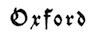
\includegraphics[width=2.5cm]{oxfordname2.png} \\

        \vspace{1cm}
        {\large At the Clarendon Press} \\
        {\large MDCCCLXXXVIII}
    \end{center}
\end{titlingpage}

\clearpage
\thispagestyle{empty}
\vspace*{\fill}

\noindent
\textbf{Reprint Edition 1977 by Arno Press Inc.} \\
Reprinted from a copy in The Princeton University Library. \\
\textit{International Folklore} -- Advisory Editor: Richard M. Dorson.

\vspace{0.5cm}
\noindent

\includegraphics[width=1.5cm]{arno1.png} \\
ARNO PRESS \\
A New York Times Company \\
New York / 1977

\vspace{0.5cm}
\noindent
Library of Congress Cataloging in Publication Data \\
Perrault, Charles, 1628-1703. \\
Popular tales. (International folklore) \\
Reprint of the 1888 ed. published by the Clarendon Press, Oxford. \\
ISBN 0-405-10118-X

\clearpage
\tableofcontents*

\clearpage
\chapter{PREFACE}
\notechapter{PREFACE.}

% \vspace{-12pt}

\textls[-25]{

  This edition of the stories of Perrault is intended partly
as an introduction to the study of Popular Tales in general. The text of
the prose has been collated by M. Alfred Bauer with that of the
first edition (Paris, 1697), a book which probably cannot be found in
England. I have to thank M. Bauer for the kind and minute care he
has bestowed on his task. We have tried to restore the original text of
1697, with its spelling, punctuation, use of capital letters, and so
forth. One might have compared the text of Perrault\textquotesingle s
prose tales, as published in a book in 1697, with their original
form in Moetjens\textquotesingle s Recueil or Magazine. Unluckily
the British Museum only possesses the earlier volumes of the Recueil, in
which the less important stories, those in verse, were first published.
The Text of the tales in Verse has been collated, by myself and Mrs.
Ogilby, with that of the Recueil. The Paris editions of 1694 and
1695 I have never seen. In his \textquotesingle Contes en Prose de
Charles Perrault\textquotesingle{} (Jouaust, \emph{Paris, 1876}), M.
Paul Lacroix published the more important readings in which the
Recueil differed from the ultimate text. The changes shew good taste on
the part of Perrault: one or two tedious gallantries, out of
keeping with the stories, were removed by him.

  Two of the most useful books that have been read by me in
preparing this edition are M. André Lefèvre\textquotesingle s
edition of the Contes, with his bibliographical and other notes,
and the \textquotesingle Contes de Ma Mère L\textquotesingle Oye avant
Charles Perrault,\textquotesingle by the late M. Charles Deulin.
I have also read, I think, most of the modern editions of the
Contes which offer any fresh criticism or information, and
acknowledgments will be found in the proper place.

The Introduction contains a brief sketch of Perrault, and
of the circumstances in which his tales were composed and published.
Each prose story has also been made the subject of a special comparative
research; its wanderings and changes of form have been observed, and it
is hoped that this part of the work may be serviceable to students of Folklore and Mythology.

In this little book, as in all researches into tradition, I have received much aid from the writings and from the kind suggestions of M. Henri Gaidoz, and from the knowledge and experience of Mr. Alfred Nutt. It is almost superfluous to add that without the industry of such students as Herr Reinhold Köhler, M. Paul Sébillot, Mr. Ralston, M. Cosquin, and very many others, these studies of story could never have been produced.} \\

\begin{flushright}
\itshape A. L.
\end{flushright}

\chapter{INTRODUCTION.}
\notechapter{INTRODUCTION.}

\begin{flushright}
\large \itshape Charles Perrault.
\end{flushright}

In Eisen\textquotesingle s portrait of Charles Perrault, the medallion
which holds the good-natured face under the large \emph{perruque} is
being wreathed with flowers by children. Though they do not, for the
most part, know the name of their benefactor, it is children who keep
green the memory of Perrault, of the author of \emph{Puss in Boots} and
\emph{Bluebeard}. He flies for ever \emph{vivu\textquotesingle{} per ora
virum}, borne on the wings of the fabulous Goose, \emph{notre Mère
L\textquotesingle Oye}. He looked, no doubt, for no such immortality,
and, if he ever thought of posthumous fame, relied on his elaborate
\emph{Parallèle des Anciens et des Modernes} (4 vols. Paris, 1688-96).
But fate decided differently, and he who kept open the Tuileries gardens
in the interests of children for ever, owes the best of his renown to a
book in the composition of which he was aided by a child.

Though a man of unimpeached respectability of conduct, Charles Perrault
was a born Irregular. He was a truant from school, a deserter of the
Bar, an architect without professional training, a man of letters by
inclination, a rebel against the tyranny of the classics, and immortal
by a kind of accident.

He did many things well, above all the things that he had not been
taught to do, and he did best of all the thing which nobody expected him
to have done. A vivid, genial and indomitable character and humour made
him one of the best-liked men of his age, and better remembered than
people with far higher contemporary reputation than his own.

Charles Perrault, as he tells us in his \emph{MÉMOIRES} (1769, Patte,
Paris; 1 vol. in 12), was born at Paris, on January 12, 1628. At the age
of nine he was sent to the Collége de Beauvais, and was aided in his
studies by his father, at home. He was always at the head of his form,
after leaving the Sixth (the lowest) which he entered before he had
quite learned to read. He was not a prodigy of precocious instruction,
happily for himself. He preferred exercises in verse, and excelled in
these, though the gods had not made him poetical. In the class of
Philosophy he was deeply interested, wrangling with his teacher, and
maintaining, characteristically, that his arguments were better than the
stock themes, \textquotesingle because they were new.\textquotesingle{}
Thus the rebel against the Ancients raised his banner at school, where
one recruit flocked to it, a boy called Beaurin. Young Perrault and his
friend took a formal farewell of their master, and solemnly seceded to
the garden of the Luxembourg, where they contrived a plan of study for
themselves. For three or four years they read together as chance or
taste directed: this course had not in it the making of a scholar.

Perrault\textquotesingle s first literary effort was a burlesque of the
Sixth book of the Æneid, a thing rather too sacred for parody in
Scarron\textquotesingle s manner. His brother the doctor took a hand in
this labour, and Perrault says \textquotesingle the MS. is on the shelf
where there are no books but those written by members of the
Family.\textquotesingle{} The funniest thing was held to be the couplet
on the charioteer Tydacus, in the shades,

\begin{verse}
\small
Qui, tenant l\textquotesingle ombre d\textquotesingle une brosse, \\
Nettoyait l\textquotesingle ombre d\textquotesingle un carrosse.
\end{verse}

Perrault, as a young man, was moderately interested in the fashionable
controversy about Grace, \emph{pouvoir prochain et pouvoir éloigné}, and
the jargon of the quarrel between Port Royal and the Jesuits. His
brother, a doctor of the Sorbonne, explained the question,
\textquotesingle and we saw there was nothing in it to justify the noise
it made.\textquotesingle{} He persuaded himself, however, that this
little conference was the occasion of the \emph{Lettres Provinciales}.
The new Editor will doubtless deal with this pretension when he comes to
publish Pascal\textquotesingle s Life in the series of \emph{Grands
Ecrivains de la France}. Unlike Perrault, Pascal thought
\textquotesingle que le sujet des disputes de Sorbonne étoit bien
important et d\textquotesingle une extrême conséquence pour la
religion.\textquotesingle{}

The first of the Provincial Letters is dated January 23, 1656. Charles
Perrault was now twenty-eight. In 1651 he had taken his \emph{licences}
at Orleans, where degrees were granted with scandalous readiness.
Perrault and his friends wakened the learned doctors in the night,
returned ridiculous answers to their questions, chinked their money in
their bags,---and passed. The same month they were all admitted to the
Bar. His legal reading was speculative, and he proposed the idea of
codifying the various customs; but the task waited for Napoleon.
Wearying of the Bar he accepted a place under his brother,
Receiver-General of Paris. In this occupation he remained from 1654 to
1664. He had plenty of leisure for study, his brother had bought an
excellent library, and Perrault speaks of \textquotesingle le plaisir
que j\textquotesingle eus de me voir au milieu de tant de bons
livres.\textquotesingle{} He made verses, which were handed about and
attributed to Quinault. That poet, getting a copy from Perrault,
permitted a young lady whom he was courting to think they were his own.
Perrault claimed them, and \textquotesingle M. Quinault se trouvait un
peu embarrassé.\textquotesingle{} However, when Quinault said that a
lady was in the case, the plagiary was forgiven. Perrault afterwards
wrote a defence of his \emph{Alceste}. A trifling piece which Perrault
composed on this little affair pleased Fouquet, who had it copied on
vellum, with miniatures and gilt capitals.

In 1657 Perrault directed the construction of a house for his brother.
The skill and taste he shewed induced Colbert to make him his subaltern
in the superintendence of the Royal buildings, in 1663. A vision of a
completed Louvre, and of \textquotesingle obelisks, pyramids, triumphal
arches, and mausoleums,\textquotesingle{} floated before the mind of
Colbert. Then there would be \emph{fêtes} and masquerades to describe,
and as Chapelain recommended Perrault, who was already the author of
some loyal odes, (such as the wise write about Jubilee times,) he
finally received an elegant appointment, with 500, later 1000
\emph{livres} a year. This he enjoyed till 1683. A little Academy of
Medals and Inscriptions grew into existence: Perrault edited panegyrics
on the king, and made designs for Gobelin tapestries.

Perrault\textquotesingle s next feat was the suggestion of the peristyle
of the Louvre, introduced into the design of his brother Claude, the
architect. After the Chevalier Bernini had been summoned from Rome to
finish the Louvre, and had been treated with sumptuous hospitality, a
variety of disputes and difficulties arose, and, by merit or favour, the
plan of Perrault\textquotesingle s brother, Claude, by profession a
physician, was chosen and executed. People said \textquotesingle que
l\textquotesingle architecture devoit être bien malade,
puisqu\textquotesingle on la mettait entre les mains des
médecins.\textquotesingle{}

\textquotesingle M. Colbert asked me for news of the Academy, supposing
that I was a member. I told him that I could not satisfy him, as I had
not the honour of belonging to that company. He seemed surprised, and
said I ought to be admitted. "\textquotesingle Tis a set of men for whom
the king has a great regard, and as business prevents me from often
attending their councils, I should be glad to hear from you what passes.
You should stand at the next vacancy."\textquotesingle{} So writes
Perrault, and he did become a candidate for Immortality. But a lady had
begged the next place for an Abbé, and next time, a doctor had secured
it for a \emph{curé}. Finally, the Academy elected Perrault, he says,
without any canvass on his part. Perrault introduced election for the
Academy by ballot, and he himself invented and provided a little
balloting machine, which he does not describe. One day when the King was
being publicly rubbed down after a game at tennis, an Academician prayed
that the Academy might be allowed to read addresses to his Majesty. The
King, who had probably given some courtier the side walls and a beating,
graciously permitted the Academy to add its voice to the chorus of
flattery. Perrault now disported himself among harangues, the new
Versailles fountains, grottoes, arches of triumph, and royal devices,
his brother executing his designs. They were sunny years, and Le Roi
Soleil beamed upon the house of Perrault. But a dispute between his
brother, the receiver of taxes, and Colbert caused a coolness between
Charles Perrault and the Minister. M. Perrault also married a young lady
to please himself, not to please Colbert. But, before leaving the
service of the Minister, the good Perrault had succeeded in saving the
Tuileries gardens for the people of Paris, and for the children, when it
was proposed to reserve them to the Royal use. \textquotesingle I am
persuaded,\textquotesingle{} he said, \textquotesingle that the gardens
of Kings are made so great and spacious that all their children may walk
in them.\textquotesingle{} We owe Perrault less gratitude for aiding
Lulli, who obtained the monopoly of Opera, a privilege adverse to the
interests of Molière. If Perrault thought at all of the interests of
Molière, he probably remembered that his own brother was a physician,
and that physicians were Molière\textquotesingle s favourite butts.
\textquotesingle Il ne devait pas tourner en ridicule les bons Médecins,
que l\textquotesingle Ecriture nous enjoint
d\textquotesingle honorer,\textquotesingle{} says Perrault in his
\emph{Eloges des Hommes Illustres} (1696-1700).
Molière\textquotesingle s own influence with the king corrected the
influence of Lulli, and he obtained the right to give musical pieces, in
spite of Lulli\textquotesingle s privilege, but he did not live long to
enjoy
it\pagenote{\emph{Registre de La Grange}, p. 11.}.

Ten years afterwards Colbert became \emph{si difficile et si chagrin},
that Perrault withdrew quietly from his service. He had been employed in
public functions for twenty years (1663-1683), he was over fifty, and he
needed rest. Louvois excluded him on the death of Colbert from the
\emph{petite Académie}. He devoted himself to the education of his
children, who were \textquotesingle day-boarders\textquotesingle{} at
the colleges, and returned at night to the paternal house in the
Faubourg St. Jacques. \textquotesingle Les mœurs ne sont pas en si
grande sûreté\textquotesingle{} at a public school, Perrault thought. In
1686 he published his \textquotesingle Saint Paulin Evesque de Nole,
avec une Epistre Chrestienne sur la Penitence, et une Ode aux Nouveaux
Convertis.\textquotesingle{} (Paris, J. R. Coignard.) It is dedicated to
Bossuet, in a letter, and Perrault trusts that great poets will follow
his example, and write on sacred subjects. Happily his example was not
followed, \emph{la raillerie et l\textquotesingle amour} possessing
stronger attractions for minstrels, as Perrault complains. He throws his
stone at Comedy, which Bossuet notably disliked and condemned. But this
did not prevent Perrault, seven years later, from writing little
comedies of his own. \emph{Saint Paulin} is prettily illustrated with
vignettes on copper after Sebastien le Clerc, vignettes much better than
those which hardly decorate \emph{Histoires ou Contes du Tems passé}. An
angel appearing to Saint Paulin in gardens exactly like the parterres of
Versailles is particularly splendid and distinguished. As for the poem,
\textquotesingle qui eut assez de succès malgré les critiques de
quelques personnes d\textquotesingle esprit,\textquotesingle{} the story
is not badly told, for the legend of the Bishop has a good deal of the
air of a \emph{conte}, reclaimed for sacred purposes. The \emph{Ode aux
Nouveaux Convertis} is not a success. Perrault comparing Reason to
Faith, says that Reason makes the glories beheld by Faith disappear, as
the Sun scatters the stars. This was an injudicious admission. The
\emph{Saint Paulin} may be bought for two or three francs, while the
\emph{Histoires ou Contes}, when last sold by public auction in the
original edition (Nodier\textquotesingle s copy, at the Hamilton Sale,
May 1884), fetched £85. It is a commercial but not inaccurate test of
merit.

Perrault\textquotesingle s \emph{Mémoires} end just where they begin to
be interesting. He tells us how he read his poem \emph{Le Siècle de
Louis XIV}, to the Academy, how angrily Boileau declared that the poem
was an insult to the great men of times past, how Huet took
Perrault\textquotesingle s side, how Boileau wrote epigrams against him,
how Racine pretended not to think him in earnest, and how he defended
himself in \emph{Le Parallèle des Anciens et des Modernes}. Here close
the Memoirs, and the hero of the great Battle of the Books leaves its
tale untold.

The quarrel is too old and too futile to require a long history.
Perrault\textquotesingle s remarks on Homer, the cause of the war,
merely show that Perrault was quite out of sympathy with the heroic age
and with heroic song. He avers that, if a favourable Heaven had
permitted Homer to be born under Louis XIV, Homer would have been a much
better poet.

\begin{verse}
\small
\textquotesingle Cent défauts qu\textquotesingle on impute au siècle où
tu naquis\\
Ne profaneroient pas tes ouvrages exquis
\pagenote{\textquotesingle Exquis\textquotesingle{} is good.}

\end{verse}

Men of letters who were men of sense would have smiled and let Perrault
perorate. But men of letters are rarely men of sense, and dearly love a
brawl. M. E. de Goncourt once complained that M. Paul de St. Victor
looked at him \textquotesingle like a stuffed bird,\textquotesingle{}
because M. de Goncourt declared that Providence had created antiquity to
prevent pedagogues from starving. Boileau was not less indignant with
Perrault, who, by the way, in his poem had damned Molière with faint
praise, and had not praised La Fontaine, Racine, and Boileau at all. The
quarrel \textquotesingle thundered in and out the shadowy
skirts\textquotesingle{} of Literature for ten years. Boileau turned and
rent the architect-physician Claude Perrault in his \emph{Art Poétique}.
But Boileau, stimulated by Conti, who wrote on his \emph{fauteuil},
\textquotesingle{}\emph{tu dors, Brutus,}\textquotesingle{} chiefly
thundered in his \emph{Réflexions Critiques} on Longinus (1694).
\textquotesingle He makes four errors, out of ignorance of Greek, and a
fifth out of ignorance of Latin,\textquotesingle{} is an example of
Boileau\textquotesingle s amenities. Why Boileau should have written at
such length and so angrily on \emph{un livre que personne ne lit}, he
does not explain. Perrault kept his temper, Boileau displayed his
learning. Arnauld had the credit of making a personal peace between the
foes. Boileau suppressed some of his satirical lines (Satire X. line
459), and we now read them only in the foot-notes.
Boileau\textquotesingle s letter to Arnauld, in which he expresses his
willingness even to read \emph{Saint Paulin} for the sake of a peaceful
life, is not unamusing. \textquotesingle Faut-il lire tout \emph{Saint
Paulin}? Vous n\textquotesingle avez qu\textquotesingle à dire: rien ne
me sera difficile\textquotesingle{} (June 1694). Meanwhile Perrault, in
his comedy \emph{L\textquotesingle Oublieux}, was mocking people who
think it a fine thing \textquotesingle to publish old books with a great
many
notes\textquotesingle{}\pagenote{\emph{L\textquotesingle Oublieux} was written in 1691. It was printed
from the MS. by M. Hippolyte Lucas. \emph{Académie des Bibliophiles},
Paris, 1868.}.

But Perrault himself was about to win his own fame by publishing
versions of old traditional Fairy Tales.

The following essay traces the history and bibliography of these Tales.
Perrault\textquotesingle s last years were occupied with his large
illustrated book, \emph{Eloges des Hommes Illustres du Siècle de Louis
XIV} (2 vols. in folio. 102 portraits.) He died on May 16, 1703. His
fair enemy in the bookish battle, Madame Dacier, says
\textquotesingle{}\emph{il étoit plein de piété, de probité, de vertu,
poli, modeste, officieux, fidèle à tous les devoirs
qu\textquotesingle exigent les liaisons naturelles et acquises; et, dans
un poste considérable auprès d\textquotesingle un des plus grands
ministres que la France ait eus et qui l\textquotesingle honoroit de sa
confiance, il ne s\textquotesingle est jamais servi de sa faveur pour sa
fortune particulière, et il l\textquotesingle a toujours employée pour
ses amis}.\textquotesingle{}

Charles Perrault was a good man, a good father, a good Christian, and a
good fellow. He was astonishingly clever and versatile in little things,
honest, courteous, and witty, and an undaunted amateur. The little thing
in which he excelled most was telling fairy tales. Every generation
listens in its turn to this old family friend of all the world. No
nation owes him so much as we of England, who, south of the Scottish,
and east of the Welsh marches, have scarce any popular tales of our own
save Jack the Giant Killer, and who have given the full fairy
citizenship to Perrault\textquotesingle s \emph{Petit Poucet} and
\emph{La Barbe Bleue}.

\clearpage
\printpagenotes
\resetpagenotes

\mainmatter

\part{PERRAULT\textquotesingle S POPULAR TALES.}

\textquotesingle Madame Coulanges, who is with me till to-morrow, was
good enough to tell us some of the stories that they amuse the ladies
with at Versailles. They call this \emph{mitonner}, so she
\emph{mitonned} us, and spoke to us about a Green Island, where a
Princess was brought up, as bright as the day! The Fairies were her
companions, and the Prince of Pleasure was her lover, and they both came
to the King\textquotesingle s court, one day, in a ball of glass. The
story lasted a good hour, and I spare you much of it, the rather as this
Green Isle is in the midst of Ocean, not in the Mediterranean, where M.
de Grignan might be pleased to hear of its discovery.\textquotesingle{}

So Madame de Sévigné writes to her daughter, on the 6th of August, 1676.

The letter proves that fairy tales or \emph{contes} had come to Court,
and were in fashion, twenty years before Charles Perrault published his
\emph{Contes de Ma Mère l\textquotesingle Oye}, our
\textquotesingle Mother Goose\textquotesingle s Tales.\textquotesingle{}
The apparition of the simple traditional stories at Versailles must have
resembled the arrival of the Goose Girl, in her shabby raiment, at the
King\textquotesingle s
Palace\pagenote{Grimm, \emph{Kinder- und Hausmärchen}. No. 89.}.
The stories came in their rustic weeds, they wandered out of the cabins
of the charcoal burners, out of the farmers\textquotesingle{} cottages,
and, after many adventures, reached that enchanted castle of Versailles.
There the courtiers welcomed them gladly, recognised the truant girls
and boys of the Fairy world as princes and princesses, and arrayed them
in the splendour of Cinderella\textquotesingle s sisters,
\textquotesingle mon habit de velours rouge, et ma garniture
d\textquotesingle Angleterre; mon manteau à fleurs d\textquotesingle or
et ma barrière de diamans qui n\textquotesingle est pas des plus
indifférentes.\textquotesingle{} The legends of the country folk, which
had been as simple and rude as \emph{Peau d\textquotesingle Ane} in her
scullion\textquotesingle s disguise, shone forth like \emph{Peau
d\textquotesingle Ane} herself, when she wore her fairy garments,
embroidered with the sun and moon in thread of gold and silver. We can
see, from Madame de Sévigné\textquotesingle s letter, that the
\emph{Märchen} had been decked out in Court dress, in train and
feathers, as early as 1676. When the Princess of the Green Isle, and the
Prince of Pleasures alighted from their flying ball of crystal, in
Madame Coulanges\textquotesingle{} tale, every one cried,
\textquotesingle Cybele is descending among us!\textquotesingle{} Cybele
is remote enough from the world of \ul{fairy}, and the whole story, like
the stories afterwards published by Madame d\textquotesingle Aulnoy,
must have been a highly decorated and scarcely recognisable variant of
some old tradition.

How did the \ul{fairy tales} get presented at Court, and thence win
their way, thanks to Perrault, into the classical literature of France?
Probably they were welcomed partly in that spirit of sham simplicity,
which moved Louis XIV and his nobles and ladies to appear in Ballets as
shepherds and
shepherdesses\pagenote{\emph{Ballet des Arts, dansé par sa Majesté; le 8 Janvier, 1663.}}.
In later days the witty maidens of Saint Cyr became aweary of sermons on
\emph{la simplicité}. They used to say, by way of raillery,
\textquotesingle par simplicité je prends la meilleure
place,\textquotesingle{} \textquotesingle par simplicité \pagenote{A Paris. Par
Robert Ballard. M.DC.LXIII.} je vais me louer,\textquotesingle{}
\textquotesingle par simplicité je veux ce qu\textquotesingle il y a de
plus loin de moi sur une table.\textquotesingle{} This, as Madame de
Maintenon remarked, was \textquotesingle laughing at serious
things,\textquotesingle{} at sweet simplicity, which first brought Fairy
Tales to the Œil de
Bœuf\pagenote{\emph{Madame de Maintenon d\textquotesingle après sa Correspondance.}
Geffroy, ii. 211. Paris, 1887.}.
Mlle. L\textquotesingle Heritier in \emph{Bigarrures Ingénieuses} (p.
237) expressly says, \textquotesingle Les Romances modernes tâchent
d\textquotesingle imiter la simplicité des Romances
antiques.\textquotesingle{} It is curious that Madame de Maintenon did
not find this simplicity simple enough for her pupils at St. Cyr. On the
4th of March, 1700, when the fashion for fairy tales was at its height,
she wrote to the Comte d\textquotesingle Ayen on the subject of harmless
literature for \emph{demoiselles}, and asked him to procure something,
\textquotesingle mais non des contes de fées ou de \emph{Peau
d\textquotesingle Ane}, car je n\textquotesingle en veux
point\pagenote{\emph{Madame de Maintenon d\textquotesingle après sa Correspondance.}
Geffroy, i. 322.}.\textquotesingle{}

Indeed it is very probable that weariness of the long novels and pompous
plays of the age of Louis XIV made people find a real charm in the
stories of \emph{Cendrillon}, and \emph{La Belle au Bois Dormant}. For
some reason, however, the stories (as current in France) existed only by
word of mouth, and in oral narrative, till near the end of the century.
In 1691 Charles Perrault, now withdrawn from public life, and busy
fighting the Battle of the Books with Boileau, published anonymously his
earliest attempt at story telling, unless we reckon
\emph{L\textquotesingle Esprit Fort}, a tale of light and frivolous
character. The new story was \emph{La Marquise de Salusses, ou la
Patience de Griselidis},
\emph{nouvelle}\pagenote{Paris: de l\textquotesingle imprimerie de Jean Baptiste Coignard,
imprimeur du Roy et de l\textquotesingle Académie Françoise, rue Saint
Jacques, la Bible d\textquotesingle or, 1691. The Bibliothèque Nationale
and the Arsenal possess copies of this duodecimo of 58 pages. One of the
copies is inscribed \emph{Donné par Lautheur} 1691. (Lefèvre.
\emph{Contes de Charles Perrault}, p. 167. Paris, \emph{s. a.})}.
\emph{Griselidis} is not precisely a popular tale, as Perrault openly
borrowed his matter from Boccaccio, and his manner (as far as in him
lay) from La Fontaine. He has greatly softened the brutality of the
narrative as Boccaccio tells it, and there is much beauty in his
description of the young Prince lost in the forest, after one of those
Royal hunts in Rambouillet or Marly whose echoes now scarce reach us,
faint and fabulous as the horns of Roland or of
Arthur\pagenote{Paul de Saint Victor, \emph{Les Contes des Fées}, in \emph{Hommes et
Dieux}, p. 475. Paris, 1883.}.
Nay, there is a certain simple poetry and sentiment of Nature, in
\emph{Griselidis}, which comes strangely from a man of the Town and the
Court. The place where the wandering Prince encounters first his
shepherdess

\begin{verse}
  \small
'Clair de ruisseaux et sombre de verdure \\
Saisissait les esprits d'une secrete horreur; \\
\vin La simple et naive nature \\
\vin S'y faisoit voir si belle et si pure, \\
\vin Que mille fois il benit son erreur.'
\end{verse}

So the Prince rides on his way

\begin{verse}
  \small
\vin 'Rempli de douces reveries \\
Qu'inspirent les grands bois, les eaux et les prairies.'
\end{verse}

The sentiment is like Madame de Sévigné\textquotesingle s love of her
woods at Les Rochers, the woods where she says goodbye to the Autumn
colours, and longs for the fairy \emph{feuille} \emph{qui chante}, and
praises \textquotesingle the crystal October days.\textquotesingle{} Of
all this there is nothing in Boccaccio. Perrault, of course, does not
repeat the brutalities of the Italian tyrant, in which Boccaccio takes a
kind of pleasure, while Chaucer veils them in his kindly courtesy.

To \emph{Griselidis} Perrault added an amusing little essay on the
vanity of Criticism, and the varying verdicts of critics. In this Essay,
Perrault apparently shews us the source from which he directly drew his
matter, namely Boccaccio in the popular form of the chap-books called
\emph{La Bibliothèque Bleue}. \textquotesingle If I had taken out
everything that every critic found fault with,\textquotesingle{} he
says, \textquotesingle I had done better to leave the story in its blue
paper cover, where it has been for so many years.\textquotesingle{} Thus
Perrault borrowed from the Bibliothèque Bleue, not the Bibliothèque
Bleue, as M. Maury fancied, from
Perrault\pagenote{\emph{Les Fées du Moyen Age}, p. 101. Paris, 1843.}.

In 1694 Moetjens, the bookseller at The Hague, began to publish a little
Miscellany, or Magazine, in the form of the small Elzevir collection,
called \emph{Recueil de pièces curieuses et nouvelles, tant en prose
qu\textquotesingle en vers}. Perrault had already published \emph{Les
Souhaits Ridicules}, in a Society paper, Le Mercure Galant (Nov. 1693).
He now reprinted this piece, with \emph{Griselidis} and \emph{Peau
d\textquotesingle Ane}, in Moetjens\textquotesingle{}
\emph{Recueil}\pagenote{Recueil, 1694. \emph{Peau d\textquotesingle Ane}, p. 50. \emph{Les
Souhaits Ridicules}, p. 93. \emph{Griselidis}, p. 233.}.
These versified tales caused some discussion, and were rather severely
handled by anonymous writers in the \emph{Recueil}. In 1694, Perrault
put forth the three, with the introductions and essay, in a small
volume. Probably each tale had appeared separately, but these treasures
of the book-hunter are lost. Another edition came out, with a new
preface, in
1695\pagenote{Coignard Veuve. Paris.}.

This is the early bibliographical history, as far as it has been traced
by M. André Lefèvre, of the stories in verse. They received a good deal
of unfriendly criticism, and Perrault was said, in \emph{Peau
d\textquotesingle Ane}, to have presented the public with his own
natural covering. This witticism, rather lacking in finish, is
attributed to Boileau in an epigram published in
Moetjens\textquotesingle{} \emph{Recueil}. Boileau was still irritated
with Perrault for his conduct in the great Battle of the Books between
the Ancients and Moderns. By a curious revenge Perrault, who had blamed
Homer for telling, in the Odyssey, old wives\textquotesingle{} fables,
has found, in old wives\textquotesingle{} fables, his own immortality.
In the \emph{Parallèle}, iii. p. 117, the Abbé quotes Longinus, and his
admiration of certain hyperboles in Homer. The Chevalier, another
speaker in the dialogue, replies, \textquotesingle this sort of Homeric
hyperbole is only imitated by people who tell stories like \emph{Peau
d\textquotesingle Ane}, and introduce Ogres in seven-leagued boots
(\emph{bottes à sept lieues}).\textquotesingle{} The
\textquotesingle seven-leagued boots\textquotesingle{} are in the
Chevalier\textquotesingle s fancy an apt parallel to the prodigious
bounds made by the horses of Discord, in the Iliad. Thus, even before
Perrault began to write \ul{fairy tales}, he and Boileau had a very
pretty quarrel about \emph{Peau d\textquotesingle Ane}. Boileau happened
to remember that Zoilus of old had reviled Homer for his \emph{contes de
Vieilles}, and thus he could conscientiously treat Perrault as a new
Zoilus. In the fifth volume of his works (Paris, 1772), in which these
amenities are republished, there is a Vignette by Van der Meer
representing Homer, very old and timid, cowering behind a shield which
Boileau, like Ajax, holds up for his protection, while Perrault, in a
sword and cocked hat, throws arrows at the blind bard of Chios. The
strange thing is that they were all in the right. The Odyssey, as
Fénelon\textquotesingle s Achilles tells Homer in Hades, and as Perrault
knew, is a mass of popular tales, but then these are moulded by the
poet\textquotesingle s art into an epic which Boileau could not
over-praise\pagenote{\emph{Dialogues des Morts par feu Messire François de Salignac de la
Motte Fénelon}, vol. i. p. 23. Paris, 1718.
\textquotesingle L\textquotesingle autre n\textquotesingle est
qu\textquotesingle un amas de contes de vieilles.\textquotesingle{}
Achilles thus anticipates Gerland\textquotesingle s \emph{Altgriechische
Märchen in der Odyssee}.}.

In the edition of his stories in verse, published in 1695, Perrault
replied to the criticisms that reached him, \textquotesingle I have to
do,\textquotesingle{} he said, \textquotesingle with people who can only
be moved by Authority, and the example of the
Ancients;\textquotesingle{} meaning Boileau and the survivors of the
great literary feud. Perrault therefore adduces old instances of
classical \emph{contes}, the \emph{Milesian Tales}, and \emph{Cupid and
Psyche} in Apuleius. \textquotesingle The Moral of \emph{Cupid and
Psyche},\textquotesingle{} he says, \textquotesingle I shall compare to
that of \emph{Peau d\textquotesingle Ane}, when once I know what it
is.\textquotesingle{} Then he declares that his Contes have abundance of
moral, which is true, but there are morals even in \emph{Cupid and
Psyche}. He sketches, very pleasantly, the enjoyment of children in
those old wives\textquotesingle{} fables; \textquotesingle on les voit
dans la tristesse et dans l\textquotesingle abattement tant que le héros
ou l\textquotesingle héroïne du conte sont dans le malheur, et
s\textquotesingle écrier de joie quand le temps de leur bonheur
arrive.\textquotesingle{} Indeed this was and is the best apology for M.
Perrault of the French Academy, when he stooped his great perruque to
listen to his little boy\textquotesingle s repetition of his
nurse\textquotesingle s stories, and recorded them in the chronicles of
Mother Goose.

Had Perrault only written \emph{contes} in verse, it is probable that he
would now be known chiefly as an imitator of La Fontaine. Happily he
went further, and printed seven stories in prose. It is by these that he
really lives, now that his architectural exploits, his sacred poems, his
Defence of the Moderns, are all forgotten save by the learned. His
Fairies have saved him from oblivion, and the countless editions and
translations of his \emph{Contes de Ma Mère L\textquotesingle Oye}, have
won him
immortality\pagenote{Contes de Ma Mère L\textquotesingle Oye is the title on the
frontispiece. The term occurs in Loret, \emph{La Muse Historique}.
(Lettre V. 11 Juin, 1650.)}

\begin{verse}
  \small
\enquote{Quelquefois, cependant, c'est ce petit Marmot \\
Qui fera le bonheur de toute la famille!}
\end{verse}

The tales in prose appeared in Moetjens\textquotesingle{} \emph{Recueil}
in the following order: In 1696, in the second part of Volume V, came
\emph{La Belle au Bois Dormant} (our enquote{Sleeping
Beauty}); and in 1697 (Vol. V. part 4), came \emph{Le
Petit Chaperon Rouge} (\textquotesingle Red Riding
Hood\textquotesingle), \emph{La Barbe Bleue}
(\textquotesingle Blue-beard\textquotesingle), \emph{Le Maistre Chat, ou
le Chat Botté} (\textquotesingle Puss in Boots,\textquotesingle{} or
\textquotesingle The Master Cat\textquotesingle), \emph{Les Fées}
(\textquotesingle The Fairy\textquotesingle), \emph{Cendrillon, ou la
petite pantoufle de verre}
(\textquotesingle Cinderilla,\textquotesingle{} in the older English
versions, now \textquotesingle Cinderella\textquotesingle), \emph{Riquet
à la Houppe} (\textquotesingle Riquet of the Tuft\textquotesingle), and
\emph{Le Petit Poucet} (\textquotesingle Hop o\textquotesingle{} My
Thumb, Little Thumb\textquotesingle).

While Moetjens was producing these in his Miscellany, there was
published in Paris, at Perrault\textquotesingle s
bookseller\textquotesingle s (Guignard), a little volume called
\emph{Bigarrures Ingénieuses, ou Recueil de diverses Pièces galantes en
prose et en vers}. The author was Mlle. L\textquotesingle Heritier de
Villaudon, a relation of Perrault\textquotesingle s. It is to his
daughter, a Mademoiselle Perrault, that she addresses her first piece,
\emph{Marmoisan ou l\textquotesingle Innocente Tromperie}. The author
says she was lately in a company where people began to praise M.
Perrault\textquotesingle s \emph{Griselidis}, \emph{Peau
d\textquotesingle Ane} and \emph{Les Souhaits}. They spoke also of
\textquotesingle the excellent education which M. Perrault gives his
children, of their ingenuity, and finally of the \emph{Contes naifs}
which one of his young pupils has lately written with so much charm. A
few of these stories were narrated and led on to
others.\textquotesingle{} \emph{Marmoisan} is one of the others, and
Mlle. L\textquotesingle Heritier says she told it, \textquotesingle avec
quelque broderie qui me vint sur le champ dans
l\textquotesingle esprit.\textquotesingle{} The tale is, indeed, all
embroidery, beneath which the original stuff is practically
lost\pagenote{In her \emph{Moralité}, Mlle. L\textquotesingle Heritier says,---

\begin{verse}
  \small
\enquote{Cent fois ma nourrice ou ma mie \\
M'ont fait ce beau recit le soir pres des tisons, \\
Je n'y fais qu'ajouter un peu de broderie.}
\end{verse}
}
But the listener asked the narrator to offer it \enquote{à ce
jeune Conteur, qui occupe si spirituellement les amusemens de son
enfance.}

In a later page she wonders that the Contes should have been
\textquotesingle handed to us from age to age, without any one taking
the trouble to write them out.\textquotesingle{} Then she herself takes
the trouble to write the story of Diamonds and Toads, a story known in a
rough way to the Kaffirs---and hopelessly spoils it by her
\emph{broderie}, and by the introduction of a lay figure called
\emph{Eloquentia Nativa} (\emph{Les Enchantemens de
l\textquotesingle Eloquence}, ou \emph{Les Effets de la Douceur}). One
has only to compare Mlle. L\textquotesingle Heritier\textquotesingle s
literary and embroidered \emph{Eloquentia} with
Perrault\textquotesingle s \emph{Les Fées} (the original of our
\emph{Diamonds and Toads}), to see the vast difference between his
manner, and that of contemporary \emph{conteurs}. Perrault would never
have brought in a Fairy named \emph{Eloquentia Nativa}. Mlle.
L\textquotesingle Heritier\textquotesingle s \emph{Eloquentia} (1696)
was in the field before \ul{Perrault\textquotesingle s} unembroidered
version, \emph{Les Fées}, which appeared in Moetjens\textquotesingle{}
\emph{Recueil} in 1697. The Lady writes:

{\textquotesingle Cent et Cent fois ma Gouvernante} {Au lieu de Fables
d\textquotesingle animaux\pagenote{The \emph{Fables d\textquotesingle animaux} are probably even older than
\emph{contes} \emph{Diamonds and Toads}. A Mouse and a Frog, as well as
the Old Woman who survives as \emph{La Fée}, take part in the tale as
the Kaffirs tell it in \emph{The Story of Five Heads}, in
Theal\textquotesingle s \emph{Kaffir Folk Lore}, pp. 48, 49. The Kaffir
story slides into a form of \emph{Beauty and the Beast}. By some
unexplained accident a story of Mlle.
L\textquotesingle Heritier\textquotesingle s
\emph{L\textquotesingle Adroite Princesse} slipped into editions of
Perrault\textquotesingle s \emph{Contes}, in 1721, if not earlier, and
holds its place even now.}
{M\textquotesingle a raconté les traits moraux} {De cette Histoire
surprenante.\textquotesingle{}}

Here, then, is Mlle. L\textquotesingle Heritier speaking of one of
Perrault\textquotesingle s children who has written the fairy tales,
\textquotesingle with so much charm.\textquotesingle{} At this very time
(1696-1697), \ul{fairy tales}, \textquotesingle written with much
charm,\textquotesingle{} in prose, and without the
author\textquotesingle s name, were appearing in
Moetjens\textquotesingle{} \emph{Recueil}. In 1697 these prose
\emph{contes} were collected, published, and declared to be by P.
Darmancour, Perrault\textquotesingle s little boy, to whom the
\emph{Privilége du Roy} is
granted\pagenote{\emph{Histoires ou Contes du Tems Passé, avec des Moralités.} A Paris.
Chez Claude Barbin, sur le second peron de la Sainte-Chapelle; au
Palais. Avec Privilége de sa Majesté, 1697. In 12\textsuperscript{o}.
230 pp. Bibliothèque de M. Cousin, 9677. The frontispiece, by Clouzier,
represents an old woman spinning, and telling tales to a man, a girl, a
little boy, and a cat which, from its broad and intelligent grin,
naturalists believe to be of the Cheshire breed. On a placard is written

\begin{center}
CONTES

DEMA

MERE

LOYE.
\end{center}

A copy, modified, of the engraving is printed on the cover of M. Charles
Deulin\textquotesingle s \emph{Les Contes de Ma Mère
L\textquotesingle Oye avant Perrault}. (Paris, Dentu, 1879.) The design
holds its own, with various slight alterations, in the English
chap-books of \emph{Mother Goose\textquotesingle s Tales}, even in the
present century. There is a vastly
\textquotesingle embroidered\textquotesingle{} reminiscence of Clouzier
in the edition edited by M. Ch. Giraud, for Perrin of Lyon, 1865.}.

Critics have often declared that Perrault merely used the
boy\textquotesingle s name as a cover for his own, because it did not
become an Academician to publish \ul{fairy tales}, above all in prose.
It may be noted that Perrault did not employ his usual publisher,
Coignard, but went to Barbin. There might also have been a hope that
little Perrault Darmancour, while shielding his father,
\textquotesingle fit parfaitement bien sa Cour en même
tems,\textquotesingle{} like \emph{Le Petit Poucet}. Considering how
Perrault\textquotesingle s other works are forgotten, and how his Tales
survive, and regarding his boy as partly their author, we may even apply
to him the Moral of \emph{Le Petit Poucet}.

\begin{verse}
  \small
'Quelquefois, cependant, c'est ce petit Marmot \\
Qui fera le bonheur de toute la famille!'
\end{verse}

The dedication, signed P. Darmancour, is addressed to Mademoiselle, and
contains very agreeable flattery of the sister of the future
Regent\pagenote{Mademoiselle was Elizabeth Charlotte d\textquotesingle Orleans, born
1676, sister of Philippe, Duc de Chartres, later Duc
d\textquotesingle Orleans, and Regent. See Paul Lacroix in \emph{Contes
de Perrault}, Paris, s. d. (1826.)}.
These motives would, indeed, account for Perrault\textquotesingle s use
of his boy\textquotesingle s name. But it had occurred to me, before
discovering the similar opinion of M. Paul Lacroix, that P. Darmancour
really was the author of the \emph{Contes}, or at least a
\emph{collaborateur}\pagenote{In the introduction to the Jouaust edition of 1876 M. Paul Lacroix has
probably gone too far in attributing to Perrault\textquotesingle s son
the complete authorship of the Tales. It is true that the title of the
Dutch reprint of 1697 describes the book as \textquotesingle par le fils
de Monsieur Perrault.\textquotesingle{} The Abbé de Villiers, however,
in his \emph{Entretiens sur les Contes des Fées} (à Paris chez Jacques
Collombat, 1699), makes one of his persons praise the stories
\textquotesingle que l\textquotesingle on attribue au fils
d\textquotesingle un célèbre Académicien,\textquotesingle{} for their
freshness and imitation of the style of nurses. Another speaker in the
dialogue, The Parisian, replies, \textquotesingle quelque estime que
j\textquotesingle aie pour le fils de l\textquotesingle Académicien,
j\textquotesingle ai peine à croire que le père n\textquotesingle ait
pas mis la main à son ouvrage,\textquotesingle{} p. 109. This opinion is
probably correct. It seems that Perrault was not troubled by attacks on
his \emph{Contes}, and, in biographical works the tales were long
attributed to his son. But M. Paul Lacroix declares that this son was
nineteen years of age when the stories appeared. This looks incredible
on the face of it. Mlle. L\textquotesingle Heritier could hardly have
said about a young man of nineteen, that he \textquotesingle occupe si
spirituellement les amusemens de son enfance\textquotesingle{} in
writing out \emph{Contes naifs}. Nor would a man of that age, in a
century too, when the young took on them manly duties so early, describe
himself in his dedicatory letter as \textquotesingle un
enfant.\textquotesingle{} M. Charles Giraud gives the
boy\textquotesingle s age as ten, without citing his authority. (Lyons
Edition of 1865, p. lxxiv.) Moreover the idea of educating a young man
of that age by making him write out \ul{fairy tales} would have seemed,
and would justly have seemed, ridiculous. We must believe that P.
Darmancour was a child when the stories were published, and we may agree
with the Abbé Villiers that the Academician \textquotesingle put a hand
to them.\textquotesingle{} M. Lacroix\textquotesingle s authority is the
discovery by M. Jal of the birth of Pierre Perrault, a son of Charles,
who would have been nineteen in 1697. (Jal\textquotesingle s
\emph{Dictionnaire Critique}, p. 1321.) But Jal did not find the
register of baptism of Mademoiselle Perrault. It follows that he may
have also failed to find that of other young Perraults, including
\textquotesingle P. Darmancour.\textquotesingle{} Each of
Perrault\textquotesingle s first sons (May 25, 1675; Oct. 20, 1676), was
called Charles, the second had a Samuel added to the name. Perrault may
also have had two or more Pierres; in any case, unless P. Darmancour
were an idiot, his education could not have been conducted by making him
write out nursery tales at nineteen.}.
The naïveté, and popular traditional manner of their telling, recognised
by all critics, and the cause of their popularity, was probably given by
the little lad who, as Mlle. L\textquotesingle Heritier said, a year
before the tales were published, \textquotesingle a mis depuis peu les
Contes sur le papier avec tant
d\textquotesingle agrément.\textquotesingle{} The child, according to
this theory, wrote out, by way of exercise, the stories as he heard
them, not from \emph{brodeuses} in Society, but from his Nurse, or from
old women on his father\textquotesingle s estates. The evidence of
Madame de Sévigné and of Mlle. L\textquotesingle Heritier, as well as
the testimony of the \emph{contes} which ladies of rank instantly took
to printing, shews how the stories were told in Society. Allegorical and
other names were given to the characters, usually nameless in
\emph{Märchen}. Historical circumstances were introduced, and references
to actual events in the past. \emph{Esprit} raged assiduously through
the narratives. Moreover the traditional tales were so confounded that
Madame d\textquotesingle Aulnoy, in \emph{Finette Cendron}, actually
mixes \emph{Cinderella} with \emph{Hop o\textquotesingle{} My
Thumb}\pagenote{Even in the popular mouth almost any formula may glide into almost any
other, and there is actually a female Hop o\textquotesingle{} My Thumb
in Aberdeenshire \ul{folklore.} But Madame
d\textquotesingle Aulnoy\textquotesingle s seems a wanton confusion. The
Aberdeen female \emph{Hop o\textquotesingle{} My Thumb} is \emph{Malty
Whuppy}, Folk Lore Journal, p. 68, 1884. For \emph{Finette Cendron}, see
\emph{Nouveaux Contes des Fées}, par Madame D------, Amsterdam, Roger,
1708.}.

Contrast with these refinements, these superfluities, and incoherences,
the brevity, directness, and simplicity of \emph{Histoires et Contes du
Tems passé}. They have the touch of an intelligent child, writing down
what he has heard told in plain language by plain people. They exactly
correspond, in this respect, to the Hindoo \ul{folk tales} collected
from the lips of Ayahs by Miss Maive Stokes, who was a child when her
collection was published.

But, if the little boy thus furnished the sketch, it is indubitable that
the elderly Academician and \emph{beau esprit} touched it up, here
toning down an incident too amazing for French sobriety and logic, there
adding a detail of contemporary court manners, or a hit at some foible
or vanity of men. \textquotesingle Livre unique entre tous les
livres,\textquotesingle{} cries M. Paul de St. Victor,
\textquotesingle mêlé de la sagesse du vieillard et de la candeur de
l\textquotesingle enfant!\textquotesingle{} This delightful blending of
age and youth (which here \emph{can} \textquotesingle live
together\textquotesingle) is probably due to the collaboration we
describe.

Were it a pious thing to dissect Perrault\textquotesingle s
\emph{Contes}, as Professors of all nations mangle the sacred body of
Homer, we might actually publish a text in which the work of the
original Darmancour and of the paternal \emph{Diaskeuast} should be
printed in different characters. Without carrying mere guess-work to
this absurd extent, cannot one detect the older hand in places like
this,---the Ogre\textquotesingle s wife finds that her husband has
killed his own children by misadventure: \textquotesingle Elle commenca
par s\textquotesingle évanouir (car c\textquotesingle est le premier
expédient que trouvent presque toutes les femmes en pareilles
rencontres)\textquotesingle? One can almost see the Academician writing
in that sentence on the margin of the boy\textquotesingle s copy. Again,
at the end of \emph{Le Petit Poucet}, we read that he made a fortune by
carrying letters from ladies to their lovers, \textquotesingle ce fut là
son plus large gain. Il se trouvoit quelques femmes qui le chargeoient
de lettres pour leurs maris, mais elles le payoient si mal, et cela
alloit à si peu de chose, qu\textquotesingle il ne daignoit mettre en
ligne de conte ce qu\textquotesingle il gagnoit de ce
côté-là.\textquotesingle{} That is the Academician\textquotesingle s
jibe, and it is he who makes Petit Poucet buy Offices
\textquotesingle de la nouvelle création pour sa
famille.\textquotesingle{} \textquotesingle You never did that of your
own wit,\textquotesingle{} as the Giant says to the Laddie in the Scotch
story, \emph{Nicht}, \emph{Nought}, \emph{Nothing}. But
\textquotesingle Anne, ma sœur Anne, ne vois-tu rien
venir?\textquotesingle{} \textquotesingle Je ne vois rien que le Soleil
qui poudroye et l\textquotesingle herbe qui verdoye!\textquotesingle{}
or \textquotesingle Tire la \ul{chevillette}, le bobinette
cherra,\textquotesingle{} or \textquotesingle Elle alla donc bien loin,
bien loin, encore plus loin\textquotesingle; \emph{there} the child is
listening to the old and broken voice of tradition, mumbling her ancient
burden while the cradle rocks, and the spinning-wheel turns and hums.

It is to this union of old age and childhood, then, of peasant memories,
and memories of Versailles, to this kindly handling of venerable
legends, that Perrault\textquotesingle s \emph{Contes} owe their
perennial charm. The nursery tale is apt to lose itself in its
wanderings, like the children in the haunted forest; Perrault supplies
it with the clue that guides it home. A little grain of French common
sense ballasts these light minions of the Moon, the elves; with a little
toss of Court powder on the locks, \emph{pulveris exigui jactu}, he
tames the wild \emph{fée} into the Fairy Godmother, a grande dame de par
le monde, with an agate crutch-handle on her magic wand.
\textquotesingle His young Princesses, so gentle and so maidenly, have
just left the convent of Saint Cyr. The King\textquotesingle s sons have
the proud courtesy of Dauphins of France: the Maids of Honour, the
Gentlemen of the Bed-chamber, the red-nosed Swiss guards, sleep through
the slumber of the \emph{Belle au Bois
Dormant}\pagenote{Paul de Saint Victor, \emph{Hommes et Dieux}, p. 474.}.\textquotesingle{}

They are all departed now, Dukes and Vicomtes and Princes, the Swiss
Guards have gone, that made the best end of any, the hunting horn is
still, and silent is the spinning wheel. The great golden coaches have
turned into pumpkins again, the coachman has jumped down from his box,
and hidden in his rat-hole, the Dragoon and the Hussar have clattered
off for ever, the Duchesses dance no more in the minuet, nor the fairies
on the haunted green. But in Perrault\textquotesingle s enchanted book
they are all with us, figures out of every age, the cannibal ogre that
little Zulu and Ojibbeway children fear not unreasonably; the starving
wood-cutter in the famines Racine deplored; the Princess, so like
Mademoiselle; the Fairy Godmother you might mistake for Madame
d\textquotesingle Epernon; the talking animals escaped from the fables
of days when man and beast were all on one level with gods, and winds,
and stars. In Perrault\textquotesingle s fairy-land is room for all of
them, and room for children too, who wander hither out of their own
world of fancy, and half hope that the Sleeping Beauty dwells behind the
hedge of yew, or think to find the dangerous distaff in some dismantled
chamber.

The \emph{Histoires et Contes du Tems Passé} must clearly have been
successful, though scant trace of their success remains in the criticism
of the
time\pagenote{\emph{L\textquotesingle Histoire de Mélusine} (Barbin, Paris, 1698) is
dedicated like \emph{Histoires et Contes du Tems Passé} to
\emph{Mademoiselle}. The author says, \textquotesingle Si tost que la
plus célèbre des Fées a sceu que votre Altesse Royale avoit eu la bonté
de donner de favourables audiences aux Fées du bas ordre, et
qu\textquotesingle elle avoit pris quelque plaisir au recit de leurs
avanteures,\textquotesingle{} she came forward and asked Mademoiselle to
patronise her own. A burlesque \textquotesingle Privilége en faveur des
Fées dans ce temps où l\textquotesingle on a tant
d\textquotesingle engouement pour les Contes des Fées\textquotesingle{}
ends the volume.}.
We may measure it by the fleet of other books of fairy tales which
\textquotesingle pursue the triumph and partake the
gale.\textquotesingle{} The \emph{Contes de Fées} of Mad. La Comtesse de
M------ (Murat) were published by Barbin in 1698. How little the manner
resembles Perrault\textquotesingle s \textquotesingle fairy-way of
writing,\textquotesingle{} how much it deserves the censure of the Abbé
de Villiers, may be learned from the opening sentence of \emph{Le
Parfait Amour}. \textquotesingle Dans un de ces agréables pais qui sont
dependans de l\textquotesingle Empire des Fées, regnoit la redoutable
Danamo, elle estoit scavante dans son art, cruelle dans ses actions, et
glorieuse de l\textquotesingle honneur d\textquotesingle estre descendue
de la célèbre Calipso, dont les charmes eurent la gloire et le pouvoir
en arrestant le fameux Ulisse, de triompher de la prudence des
vainqueurs de Troye.\textquotesingle{}

The second story, \emph{Anguillette}, is so far natural, that it
contains a friendly Eel (as in the Mangaian legend of the Eel-lover of
Ina); but this Eel is a fairy, condemned to wear the form of a fish, for
certain days in each month. These narratives are almost unreadable, and
scarcely keep a trace of the popular tradition. The tales of Madame
d\textquotesingle Aulnoy, on the other hand, introduced the \emph{White
Cat}, the \emph{Yellow Dwarf}, \emph{Finette Cendron}, and \emph{Le
Mouton} to literature and the stage, where they survive in pantomime and
\emph{féerie}. \emph{Beauty and the Beast} first appears, at the
immoderate length of three hundred and sixty-two pages, in \emph{Les
Contes Marins} (La Haye, 1740) by Madame de Villeneuve.

Literary Fairy Tales flourished all through the eighteenth century in
the endless \emph{Cabinet de Fées}. As for Perrault\textquotesingle s
Tales, they were republished at the Hague, in 1742, with illustrations
by Fokke. In 1745, they appeared, with Fokke\textquotesingle s
vignettes, and with an English translation. An English version,
translated by Mr. Samber, printed for J. Pote, was advertised, Mr.
Austin Dobson tells me, in the \emph{Monthly Chronicle}, March 1729.
There have been innumerable editions, often splendidly equipped and
illustrated, down to the present date. This little book alone, of all
Charles Perrault\textquotesingle s labours, has won \textquotesingle the
land of matters unforgot.\textquotesingle{} Odysseus, Figaro, and
Othello are not more certain to be immortal than Hop o\textquotesingle{}
my Thumb, Puss in Boots, and Blue Beard, the heroes whom Charles Nodier
so pleasantly called \textquotesingle the Ulysses, the Figaro, and the
Othello of children.\textquotesingle{}

{Fairies and Ogres.}

The stories of Perrault are usually called \textquotesingle Fairy
Tales,\textquotesingle{} and they deserve the name more than most
\emph{contes}, except the artificial contemporary tales, because in them
Fairies or Fées do play a considerable part. Thus there were seven
Fairies, and an old one \textquotesingle supposed dead or
enchanted,\textquotesingle{} in the \emph{Sleeping Beauty}. There is a
Fairy Godmother in \emph{Cinderella}, and, as will be shown in the study
on \emph{Cinderella}, she takes the part usually given, in traditional
versions, to a cow, a sheep, or a dead mother who has some mystic
connection with the beast. The same remarks apply to the Fairy Godmother
in \emph{Peau d\textquotesingle Ane}. She, too, does for the heroine
what beasts do in purely popular European variants, and in analogous
tales from South Africa.

The fairies in \emph{Riquet of the Tuft} are of little importance, as
the narrative is not really traditional, but of literary invention for
the most part. The fairy in \emph{The Two Wishes} is not a fairy in the
South African variants where divers magical or animal characters appear,
nor can \emph{Mother Holle} in Grimm (24) be properly styled a fairy.
Thus, of all Perrault\textquotesingle s Fairies only the Fairies of the
\emph{Sleeping Beauty} (repeated in \emph{Riquet of the Tuft}) answer to
Fairies as they appear in genuine popular traditions, under such names
as Moirai, or Hathors, in ancient Greek, and Egyptian versions. These
beings attend women in child-bed, as they attended Althea when she bore
Meleager, and they predict the fortunes of the infant.

Perrault\textquotesingle s fairy godmothers (unlike the fairies of real
legend) are machinery of his own, and even he dispenses with Fairies
altogether in \emph{Blue Beard}, \emph{Hop o\textquotesingle{} my
Thumb}, and \emph{Puss in Boots}; while in \emph{Les Trois Souhaits} the
mythological machinery of the classics is employed, and Jupiter does
what a fairy might have done. It is true that the key of the forbidden
door, in \emph{Blue Beard}, is said to be \emph{Fée}; but this only
means that, like the seven-leagued Boots in \emph{Hop
o\textquotesingle{} my Thumb} (\textquotesingle elles estoient
Fées\textquotesingle), the key has magical qualities. The part of
Fairies, then, is very restricted, even in Perrault, while, in
traditional \emph{Märchen} all over the world, Fairies or beings
analogous to the Fairies appear comparatively seldom.

In spite of this the Fairies have so successfully asserted their title
over popular tales, that a few words on their character and origin seem
not out of place. Fairies are doubtless much older than their name; as
old as the belief in spirits of woods, hills, lonely places, and the
nether world. The familiar names, \emph{fées}, \emph{fades}, are
apparently connected with \emph{Fatum}, the thing spoken, and with
\emph{Fata}, the Fates who speak it, and the God \emph{Fatuus}, or
Faunus, and his sister or wife
\emph{Fatua}\pagenote{Fauno fuit uxor nomine Fatua. Justin, xliii. I. Preller, \emph{R. M.} I.
385.}.
Preller quotes the \emph{Fatuae} as spiritual maidens of the forests and
elements, adding the other names of \emph{Sagae} and \emph{Sciae}, to
Fatuae, and
Fata\pagenote{\emph{Römische Mythologie}, i. 100. Berlin, 1881.}.
He compares the Slavonic Wilis: and, to be brief, the Apsaras of India,
the Nereids of ancient and modern Greece, and the Good Ladies and
Fairies of Scotland, with many of the Melanesian Vuis, forest-haunting
spirits, are all of the same class, are fairy beings informing the
streams and wilds. To these good folk were ascribed gifts of prophecy,
commonly exercised beside the cradle of infancy, \emph{deabus illis quae
fata nascentibus canunt, et dicuntur
Carmentes}\pagenote{Preller, \emph{op. cit.} ii. 194, quoting Tertullian, \emph{De An.} 39,
and Augustine, \emph{Civitas Dei}, iv. 11.}.
As Maury
shows\pagenote{\emph{Les Fées du Moyen Age}, p. 13. Paris, 1843.},
the local Fairies of Roman Gaul were propitiated with altars:

FATIS\\
DERVONIBUS\\
V. S. L. M. M. RVFNVS\\
SEVERVS.

Just as the Scotch Fairies are euphemistically styled
\textquotesingle The Good Folks,\textquotesingle{} \textquotesingle The
People of Peace,\textquotesingle{} the \textquotesingle Good
Ladies,\textquotesingle{} so it befell the daughter of Faunus. She was
styled \textquotesingle The Good Goddess,\textquotesingle{} and her real
name was
tabooed\pagenote{Quam quidam, quod nomine dici prohibitum fuerat, \emph{Bonam Deam}
appellatam volunt. Servius, \emph{Æneid}, viii. 315.}.

It was natural that when Christianity reached Gaul, where the native
spirits of woods and wells had acquired the name of \emph{Fata}, these
minor goddesses should survive the official heathen religion. The
temples of the high gods were overthrown, or turned into churches, but
who could destroy all the woodland fanes of the Fata, who could uproot
the dread of them from the hearts of peasants? Saints and Councils
denounced the rural offerings to fountains and the roots of trees, but
the secret shame-faced worship lasted deep into the middle
ages\pagenote{Maury, \emph{Les Fées du Moyen Age}, pp. 15, 16, and his authorities in
the \emph{Capitulaires} and \emph{Life of Saint Eloi}.}.
It is conjectured by Maury, as by Walckenaer (\emph{Lettres sur les
Contes de Fées}; Paris, 1826), that the functions of prophetic Gaulish
Maidens and Druidesses were confused with those of the Fairies.
Certainly superstitious ideas of many kinds came under the general head
of belief in \emph{Fata}, \emph{Faes}, \emph{Fadae}, and the \emph{Fées}
of the forest of Broceliande. The \emph{Fées} answered, as in the
\emph{Sleeping Beauty}, to Greek \emph{Moirai} or Egyptian
\emph{Hathors}\pagenote{Amyot, in his Plutarch, actually renders \emph{Moirai} by \emph{Fées}
(1567).}.
They nursed women in labour: they foretold the fate of children. It is
said that when a Breton lady was giving birth to a child, a banquet for
the \emph{Fées} was set in the neighbouring
chamber\pagenote{Maury, p. 31.}.
But, in popular superstition, if not in Perrault\textquotesingle s
tales, the \emph{Fées} had many other attributes. They certainly
inherited much from the pre-Christian idea of Hades. In the old MS.
\emph{Prophesia Thomae de
Erseldoun}\pagenote{Scott, \emph{Border Minstrelsy}, iii. 381.}
the subterranean fairy-world is the under-world of pagan belief. In the
mediæval form of Orpheus and Eurydice (\emph{Orfeo and Heurodis}), it is
not the King of the Dead, but the king of Fairy that carries off the
minstrel\textquotesingle s bride. Fairyland, when Orpheus visits it, is
like Homer\textquotesingle s Hades.

\begin{verse}
  \small
'And sum thurch the bodi hadde wounde \\
Wives ther lay on childe bedde \\
Sum dede and sum awedde.'
\end{verse}

In the same way Chaucer calls Pluto \textquotesingle King of
Fayrie,\textquotesingle{} and speaks of \textquotesingle Proserpine and
all her fayrie,\textquotesingle{} in the
\emph{Merchant\textquotesingle s Tale}. Moreover Alison Pearson, when
she visited Elfland, found there many of the dead, among them Maitland
of Lethington, and one of the Buccleughs. For all this dealing with
fairies and the dead was Alison burned (Scott, \emph{Border Minstrelsy},
ii. 137-152).

Because the mediæval Fairies had fallen heir to much of the
pre-Christian theory of Hades, it does not follow, of course, that the
Fairies were originally ancestral ghosts. This origin has been claimed
for them, however, and it is pointed out that the stone arrow-heads of
an earlier race are, when found by peasants, called
\textquotesingle elf-shots,\textquotesingle{} and attributed to the
Fairies. Now the real owners and makers were certainly a race dead and
gone, as far as a race can die. But probably the ownership of the arrows
by elves is only the first explanation that occurs to the rural fancy.
On the other hand, it is candid to note that the Zulu Amatongo,
certainly \textquotesingle ancestral ghosts,\textquotesingle{} have much
in common with Scotch and Irish fairies. \textquotesingle It appears to
be supposed,\textquotesingle{} says Dr. Callaway, \textquotesingle that
the dead become "good people," as the dead among the Amazulu become
Amatongo, and, in the funeral processions of the "good people" which
some profess to see, are recognised the forms of those who have lately
died, as Umkatshana saw his relatives among the
Abapansi,\textquotesingle{} and as Alison saw Maitland of Lethington and
Buccleuch in Elfland. This Umkatshana followed a deer into a hole in the
ground, where he found dead men whom he
knew\pagenote{\emph{Nursery Tales of the Zulus}, p. 317; \emph{Amatongo}, p. 227.}.
Compare Campbell, \emph{Tales from the West Highlands}, ii. 56, 65, 66,
106, where it is written, \textquotesingle the Red Book of Clanranald is
said not to have been dug up, but found \emph{on} the moss. It seemed as
if the ancestors sent it.\textquotesingle{}

Those rather gloomy fairies of the nether-world have little but the name
in common with the fairies of Herrick, of the \emph{Midsummer
Night\textquotesingle s Dream}, and of Drayton\textquotesingle s
\emph{Nymphidia}. The gay and dancing elves have a way, in Greece, of
making girls \textquotesingle dance with the Nereids\textquotesingle{}
till they dance themselves to death. In the same way it is told of Anne
Jefferies, of St. Teath in Cornwall (born 1626), that one had seen her
\textquotesingle dancing in the orchard, among the trees, and that she
informed him she was then dancing with the Fairies.\textquotesingle{}
She lived to be seventy, in spite of the Fairies and the local
magistrates who tried her case (Scott, \emph{B.M.} ii. 156).

Perrault\textquotesingle s fairies do not wed mortal men, in this
differing from the Indian Apsaras, and the fairies of New Zealand and of
Wales. (Taylor\textquotesingle s \emph{New Zealand}, p. 143. Compare
story of Urvasi and Pururavas, Max Müller, \emph{Selected Essays}, i.
408. A number of other examples of Fairy loves, including one from
America, is given in \emph{Custom and Myth}, pp. 68-86.)

On a general view of the evidence, it appears as if the fashion for
\ul{fairy} tales, in Perrault\textquotesingle s time, had made rather
free with the old \emph{Fata} or \emph{Fées}. Perrault sins much less
than the Comtesse d\textquotesingle Aulnoy, or the Comtesse de Murat,
but even he brings in a \emph{Fatua ex machina} where popular tradition
used other expedients.

As to the Ogres in Perrault, a very few words may suffice. They are
simply the survival, in civilised \ul{folklore}, of the cannibals,
\emph{Rakshasas}, \emph{Weendigoes}, and man-eating monsters who are the
dread of savage life in Africa, India, and America. Concerning them,
their ferocity, and their stupidity, enough will be said in the study of
\emph{Le Petit Poucet}. As to the name of Ogre, Walckenaer derives it
from \emph{Oigour}, a term for the Hungarian invaders of the ninth
century, a Tartar
tribe\pagenote{In popular French versions the Ogre is often called \emph{Le Sarrasin}
to this day (Sébillot in \emph{Mélusine}, May 5, 1887).}.
Hence he concludes that the Ogre-stories are later than the others,
though, even if \textquotesingle Ogre\textquotesingle{} meant
\textquotesingle Tartar,\textquotesingle{} only the name is recent, and
the Cannibal tales are of extreme antiquity. Littré, on the other hand,
derives \emph{ogre} from \emph{Orcus}, \emph{cum Orco rationem habere}
meaning to risk one\textquotesingle s life. Hop o\textquotesingle{} my
Thumb certainly risked his, when he had to do \textquotesingle cum
Orco,\textquotesingle{} if Orcus be \emph{Ogre} (\emph{Lettres sur les
Contes de Fées}, p. 169-172).

\chapter[NOTES ON THE SEVERAL TALES BY PIERRAULT]{NOTES ON THE SEVERAL TALES BY PERRAULT\\[1ex] \large \itshape AND THEIR VARIANTS.}
\notechapter{NOTES ON THE SEVERAL TALES BY PIERRAULT}

\section{Les Trois Souhaits.}
\notesection{Les Trois Souhaits.}

\emph{The Three Wishes.} \\

The story of \emph{The Three Wishes} is very valuable as an illustration
of the difficulties which baffle, and perhaps will never cease to
baffle, the student of popular Tales and their diffusion. The
fundamental idea is that a supernatural being of one sort or another can
grant to a mortal the fulfilment of a wish, or wishes, and that the
mortal can waste the boon. Now probably this idea might occur to any
human mind which entertained the belief in communication between men,
and powerful persons of any sort, Gods, Saints, Tree-spirits, fairies,
\emph{follets} or the like. The mere habit of prayer, universally human
as it is, contains the germs of the conception. But the notion, as we
find it in story, branches out into a vast variety of shapes, and the
problem is to determine which of these, or whether any one of these is
the original type, and whether the others have been adapted or
burlesqued from that first form, and whether these processes have been
the result of literary transmission, and literary handling, or of oral
traditions and popular fancy. Perhaps a compact statement of some (by no
means all) of the shapes of \emph{The Three Wishes} may here be
serviceable.

1. The granters of the Wishes are gods. The gift is accepted in a pious
spirit, and the desires are noble, and worthy of the donors.

This tale occurs in Ovid, \emph{Metamorphoses}, viii. 610-724. Baucis
and Philemon entertain the gods, who convert their hut into a Temple.
They \emph{wish} (the man is the speaker) to serve the gods in this
fane, and that neither may outlive the other:

\begin{verse}
\small
\vin\vin \foreignlanguage{latin}{Nec conjugis umquam \\
Busta meae videam: neu sim tumulandus ab illa.}
\end{verse}

Their wishes are fulfilled.

2. In German popular tales, this idea appears, with additions, in
\emph{Rich and Poor} (Grimm 87). Here the virtue of the good is
contrasted with the folly of the bad. The Poor man hospitably receives
our Lord, and, for his three wishes, chooses eternal happiness, health
and daily bread, and a new house. The Rich man rejects our Lord, but
getting a second chance, loses his temper, wishes his horse dead, the
saddle on his wife\textquotesingle s back, and---the saddle off again!

Now popular fancy has been better pleased with the burlesque ideas in
the second part of this fable, than with the serious moral; and most of
the tales turn on burlesque wishes, leaving the virtuous wishers out of
the story. The narrative also shews a Protean power of altering details,
the wishes vary, the power who grants the wish is different in different
\emph{Märchen}, the person whose folly wastes the wish may be the
husband, or may be the wife.

A very old form of the Wasted Wish, originally no doubt a popular form,
won its way into literature in the \emph{Pantschatantra}. The tale has
also been annexed by Buddhism, as Buddhism annexed most tales, by the
simple process of making Sakya Muni the hero or narrator of the
adventures.

The \emph{Pantschatantra} is a collection of fables in Sanskrit. In its
original form, according to Mr. Max Müller, its date can be fixed, by
aid of an ancient Persian translation, as previous to 550 {A.D.}
\textquotesingle At that time a collection somewhat like the
Pa\emph{n}katantra, though much more extensive, must have
existed\pagenote{\emph{Selected Essays}, i. 504.}.\textquotesingle{}
By various channels the stories of the \emph{Pantschatantra} reached
Persia, Arabia, Greece, and thence were rendered into Latin, and again,
were paraphrased in different vernacular languages, by literary people.
But when we find, as we do, a story in the \emph{Pantschatantra} and a
similar or analogous story in the Arabic \emph{Book of Sindibad}
(earlier than the tenth century), and again in the Greek \emph{Syntipas}
(eleventh and twelfth century), and again in Latin, or Spanish, or
French literature, we cannot, perhaps, always be sure that the tale is
derived from India through literary channels. Whoever will compare the
\emph{Wish} story of the \emph{Double-headed Weaver} in the
\emph{Pantschatantra}\pagenote{Benfey, ii. 341.}
with \emph{The Three Wishes} in the \emph{Book of Sindibad} (Comparetti.
\emph{Folk Lore Society}, 1882, p. 147), and again, with Marie de
France\textquotesingle s twenty-fourth Fable (\emph{Dou Vilain qui prist
un folet}), and yet again with Perrault\textquotesingle s \emph{Trois
Souhaits}, and, lastly, with the popular tales among
Grimm\textquotesingle s variants, will find many perplexing problems
before
him\pagenote{See \emph{Poésies de Marie de France, Poète Anglo-Normande du
xiii\textsuperscript{e} Siècle}, vol. ii. p. 140. Paris, 1820.}.
The differences in the details and in the conduct of the story are
immense. Did the various authors borrow little but the main
conception---the wasted wishes? Are the variations the result of
literary caprice and choice? Has the story travelled from India by two
channels,---(1) literary, in \emph{Pantschatantra}, and \emph{Syntipas}
with the translations; (2) oral, by word of mouth from people to people?
Are the \emph{popular} versions derived from literature, or from oral
tradition? Is the oldest literary version, that of the
\emph{Pantschatantra}, more akin to the \emph{original} version than
some of the others which meet us later? Finally, might not the idea of
wasted wishes occur independently to minds in different ages and
countries, and may not some of the versions be of independent origin,
and in no way borrowed from India? Is there, indeed, any reason at all
for supposing that so simple a notion was invented, once for all, in
India?

It is easy to ask these questions, it is desirable to bear them in mind,
so that we may never lose sight of the complexity and difficulty of the
topic. But it is practically impossible to answer them once for all.

The nature of the problem may now be illustrated by a few examples. In
the story of the \emph{Pantschatantra}, the granter of the wish (there
is but one wish) is a tree-dwelling spirit. A very stupid weaver one day
broke part of his loom. He went out to cut down a tree near the shore,
meaning to fashion it for his purpose, when a spirit, who dwelt in the
timber, cried, \textquotesingle Spare this tree.\textquotesingle{} The
weaver said he must starve if he did not get the wood, when the spirit
replied, \textquotesingle Ask anything else you
please.\textquotesingle{} The barber, being consulted, advised the
weaver to wish to be king. The weaver\textquotesingle s wife cried,
\textquotesingle No, stay as you are, but ask for two heads, and four
hands, to do double work.\textquotesingle{} He got his wish, but was
killed by the villagers, who very naturally supposed him to be a
Rakshasa, or ogre. The moral is enunciated by the barber,
\textquotesingle Let no man take woman\textquotesingle s
counsel.\textquotesingle{} The poor woman\textquotesingle s lack of
immoderate ambition might seem laudable to some moralists.

Here the peculiarities are: A tree-ghost grants the wish.

There is only one wish.

It is made on a woman\textquotesingle s advice.

It causes the death of the
wisher\pagenote{Benfey, \emph{Pantschatantra}, ii. 341.}.

The story is next found in the various forms of the \emph{Book of
Sindibad}, Greek, Hebrew, Persian, Arabic, and old Spanish, a book
mentioned by all Arabic authors of the tenth century, and of Indian and
Buddhistic
origin\pagenote{Comparetti, \emph{Book of Sindibad}, p. 3. Benfey,
\emph{Pantschatantra}, i. 38.}.
As told in the various forms of \emph{Sindibad}, the tale of \emph{The
Three Wishes} takes this shape. A man has a friendly spirit (a she-devil
in the Spanish \emph{Libro de los Engannos}), who is obliged to desert
his company, but leaves him certain formulæ, by dint of repeating which
he will have Three Wishes granted to him. The tree-spirit has
disappeared, the one wish has become three. The man consults with his
wife, who suggests that he should desire, not two heads and four hands,
but an obscene and disgusting bodily transformation of another sort. He
wishes the wish, is horrified by the result, and, on the
woman\textquotesingle s hint, asks to have all that embarrasses him
removed. The granting of the wish leaves him with \textquotesingle a
frightful \emph{minus} quantity,\textquotesingle{} and he expends the
third wish in getting restored to his pristine and natural condition.
The woman explains that she had not counselled him to desire wealth,
lest he should weary of her and desert her. This, at least, is the
conclusion in the Hebrew version, in the \emph{Parables of Sandabas}
(Deulin, \emph{Contes de Ma Mère L\textquotesingle Oye}, p. 71).

How are we to account for this metamorphosis of the story in the
\emph{Pantschatantra}? Is the alteration a piece of Arabian humour? Was
there another Indian version corresponding to the shape of the tale in
the \emph{Book of Sindibad}? The questions cannot be answered with our
present knowledge.

Another change, and a very remarkable one, occurs in the \emph{Fables}
of Marie de France. Of Marie not much is known. In the \emph{Conclusion}
of her Fables, she says---

\begin{verse}
  \small
'Au finement de cest escrit \\
K'én Romanz ai turné et dit, \\
Me numerai par remembraunce \\
Marie ai num, si sui de Fraunce.

* * * * *

Pur amur le cumte Willaume \\
Le plus vaillant de cest Royaume, \\
M'entremis de cest livre feire \\
E de l'Angleiz en Roman treire, \\
Ysopet apeluns ce livre \\
Qu'il traveilla et fist escrire; \\
De Griu en Latin le turna. \\
Li Rois Henris qui moult l'ama \\
Le translata puis en Engleiz \\
E jeo l'ai rimé en Franceiz.'
\end{verse}

That is to say, King Henry had translated into English a collection of
fables and \emph{contes} attributed to Æsop, and Marie rendered the
English into French. Now Æsop certainly did not write the story of
\emph{The Three Wishes}. The text before Marie was probably a mere
congeries of tales and fables, some of the set usually attributed to
Æsop, some from various other sources. The Latin version, the model of
the English version, was that assigned to a certain, or uncertain
Romulus, whom Marie, in her preface, calls an emperor. Probably he
borrowed from Phædrus, though he boasts that he rendered his fables out
of the Greek. M. de Roquefort thinks he did not flourish before the
eleventh or twelfth
century\pagenote{\emph{Poésies de Marie de France}, vol. ii. p. 53.}.
Who was \emph{li rois Henris} who turned the fables into
Marie\textquotesingle s English text? She lived under our Henry III.
Perhaps conjecture may prefer Henry Beauclerk, our Henry I.

In any case Marie manifestly did render the fables, or some of the
fables, in \emph{Le dit d\textquotesingle Ysopet} out of English. The
presence of English words in her French seems to raise a strong
presumption in favour of the truth of the assertion. One of these
English words occurs in her form of \emph{The Three Wishes} (Fable
xxiv), called \emph{Dou Vilain qui prist un Folet}, also \emph{Des Troiz
Oremens}, or \emph{Du Vileins et de sa Fame}. A Vilein captured a Folet
(fairy or brownie?) who granted him Three Wishes. The \emph{Folet}
resembles the tree-bogle of the \emph{Pantschatantra}. The vilein gave
two wishes to his wife. Long they lived without using the wishes. One
day, when they had a marrow bone for dinner, and found it difficult to
extract the marrow, the wife wished that her husband had---

\begin{verse}
  \small
\enquote{tel bec came li plereit \\
E cum li Huite cox aveit.}
\end{verse}

The Huite cox is an English word, woodcock, in disguise. The husband, in
a rage, wished his wife a woodcock\textquotesingle s beak also, and
there they sat, each with a very long bill, and two wishes wasted. There
Marie leaves them---

\begin{verse}
  \small
'Deus Oremanz unt ja perduz \\
Que nus n'en est a bien venuz,'
\end{verse}

\textquotesingle with two wishes lost, and no good gained
thereby.\textquotesingle{} Manifestly the third wish was expended in a
restoration of human noses to each of them. The moral is that ill
befalls them---

\begin{verse}
'qui trop creient autrui parole.'
\end{verse}

We naturally wonder whether this version was borrowed from one or other
shape of \emph{Syntipas}. If it was, did the change come in the Latin
handling of it, or in the English? Or is it not possible that the
version worked on by Marie had a \emph{popular} origin, whether derived
by oral transmission from some popular Indian shape of the story, which
had filtered through to the West, or the child of native Teutonic wit?
There seems to be no certain criterion in a case like this. Certainly no
mediæval wag was likely to alter, out of modesty, the form of the tale
in \emph{Syntipas} and its derivatives, though Marie would not have
rhymed that offensive \emph{conte} if she had met with it in the English
collection. Unluckily one is not acquainted with any version of
\emph{The Three Wishes} among backward and remote races, American or
African. If such a version were known (and it may, of course, exist), we
might argue that the tale was \textquotesingle universally
human.\textquotesingle{} There is nothing in it, as told in
\emph{Pantschatantra}, to make it seem essentially and peculiarly
Indian, and incapable of having been invented elsewhere.

A fourteenth-century version (quoted by M. Deulin from \emph{Fabliaux et
Contes} published by St. Méon, vol. iv. p. 386) amplifies all that is
least refined in \emph{Sendabar} and in \emph{Sindibad}. St. Martin
grants the wishes, there are four of them, and nobody is one penny the
better. With Philippe de Vigneules (1505-1514, the seventy-eighth of his
hundred \emph{Nouvelles}), God grants three wishes to a wedded pair. The
woman wishes a new leg for her pot, the man wishes her \emph{le pied au
ventre}, and then wishes it back again. M. Deulin found this form in
living popular tradition, at Leuze in Hainaut.

The \emph{Souhaits} of La Fontaine (\emph{Fables}, vii. 6) has this
peculiarity, that the giver of the wishes, as in Marie de France and in
\emph{Sindibad}, is a Follet or brownie, or familiar spirit, obliged to
leave his friends. He offers them three wishes; first, they ask for
wealth and are embarrassed by their riches, then for a restoration of
their mediocrity, then for wisdom.

{\textquotesingle C\textquotesingle est un trésor qui
n\textquotesingle embarrasse point.\textquotesingle{}}

La Fontaine\textquotesingle s source is obscure; had he known
\emph{Syntipas}, he might (or might not) have introduced the story among
his \emph{Contes}. Perhaps it was too rude even for that unabashed
collection.

As for Perrault, he probably drew from a popular tradition his
\emph{Aune de Boudin}. Collin de Plancy (\emph{Œuvres Choisies de Ch.
Perrault}, Paris, 1826, 240) gives a curious rustic version. Three
brothers dance with the Fairies, who offer them a wish apiece. The
eldest, as heir of the paternal property, wants no more, but, as wish he
must, asks that their calf may cure the colic of every invalid who
seizes it by the tail. (How manifestly Indian in origin is this
introduction of the sacred beast whose tail is grasped by the pious
Hindoo in his latest hours!) The youngest brother wishes the horns of
cow and calf on his brother\textquotesingle s head, the second wishes a
bull\textquotesingle s head on his brother\textquotesingle s shoulders,
and the Fairies make these wild wishes of none avail.

Manifestly the fundamental idea is capable of infinite transformations,
literary or popular: a good example is the play of \emph{Le Bucheron},
by Guichard and Philidor, acted in 1763.

The story has no connection with the three successful wishes by aid of
which the devil is defeated in a number of popular tales belonging to a
different cycle. All these are inspired, however, by the great god
Wunsch, who presides over Wishing Gates.

{\textquotesingle Would I could wish my wishes all to rest,} {And know
to wish the wish that should be best,}

says Clough, better inspired than Perrault\textquotesingle s
\emph{Bucheron}.

\section{La Belle au Bois Dormant.}
\notesection{La Belle au Bois Dormant.}

\emph{The Sleeping Beauty.} \\

The idea of a life which passes ages in a secular sleep is as old as the
myth of Endymion. But it would be difficult to name any classical legend
which closely corresponds with the story of the Sleeping Beauty. The
first incident of importance is connected with the very widely spread
belief in the Fates, or Moirai, or Hathors (in Ancient Egypt), or
fairies, who come to the bedside of Althæa, or of the Egyptian Queen, or
to the christening of the child in \emph{La Belle au Bois Dormant}, and
predict the fortunes of the newly born. In an Egyptian papyrus of the
Twentieth Dynasty there is a tale, beginning, just like
Perrault\textquotesingle s, with the grief of a king and queen, who have
no child, or at least no son. Instead of going \emph{à toutes les Eaux
du monde}, they appeal to the gods, who hear their prayers, and the
queen gives birth to a little boy. Beside his cradle the Hathors
announce that he shall perish by a crocodile, a serpent, or a dog. The
story, in Egyptian, now turns into one of the common myths as to the
impossibility of evading
Destiny\pagenote{Maspero, \emph{Contes Egyptiens}, p. 33.}.
In Perrault\textquotesingle s \emph{Conte}, of course, fairies take the
place of the Fates from whom perhaps \emph{Fée} is derived. When the
fairies have met comes in another old incident---one of them, like
Discord at the wedding of Peleus, has not been invited, and she
prophesies the death of the Princess. This is commuted, by a friendly
fay, into a sleep of a hundred years: the sleep to be caused, as the
death was to have been, by a prick from a spindle. The efforts of the
royal family to evade the doom by proscribing spindles are as futile as
usual in these cases. The Princess and all her people fall asleep, and
the story enters the cycle of which Brynhild\textquotesingle s wooing,
in the \emph{Volsung\textquotesingle s Saga}, is the heroic type.
Brynhild is thus described by the singing wood-peckers,---

{\textquotesingle Soft on the fell} {A shield-may sleepeth,} {The
lime-trees\textquotesingle{} red plague} {Playing about her.} {The
sleep-thorn set Odin} {Into that maiden} {For her choosing in war} {The
one he willed not.\textquotesingle{}}

Sigurd is bidden to awaken her, and this he does, rending her mail with
his magic sword. But the rest of the tragic story does not correspond
with \emph{La Belle au Bois Dormant}. Perrault\textquotesingle s tale
has its closest companion in Grimm\textquotesingle s \emph{Little Briar
Rose} (90), which lacks the conclusion about the wicked mother-in-law.
Her conduct, again, recurs in various tales quite unlike \emph{La Belle}
in general plot. The incident of the sleep-thorn, or something
analogous, occurs in \emph{Surya Bai} (\emph{Old Deccan Days}), where a
prick from the poisoned nail of a demon acts as the soporific. To carry
poison under the nail is one of the devices of the Voudou or Obi man in
Hayti. Surya Bai, when wakened and married by a Rajah, is the victim of
the jealousy, not of an ogress mother-in-law, but of another wife, and
\emph{that} story glides into a form of the Egyptian tale \emph{The Two
Brothers} (Maspero, i.). The sleep-thorn, or poisoned nail, takes again
in Germany the shape of the poisoned comb. \emph{Snow-white} is wounded
therewith by the jealousy of a beautiful step-mother, with a yet fairer
step-daughter (Grimm, 53). In mediæval romances, as in
\emph{Perceforest}, an incident is introduced whereby the sleeping maid
becomes a mother. Lucina, Themis, and Venus take the part of the
Fairies, Fates, or Hathors. In the Neapolitan \emph{Pentamerone} the
incident of the girl becoming a mother in her sleep is repeated. The
father (as in \emph{Surya Bai}) is a married man, and the girl, Thalia,
suffers from the jealousy of the first wife, as Surya Bai does. The
first wife wants to eat Thalia\textquotesingle s children, \emph{à
diverses sauces}, which greatly resembles Perrault\textquotesingle s
\emph{sauce Robert}. The children of Thalia are named Sun and Moon,
while those of the Sleeping Beauty are L\textquotesingle Aurore et Le
Jour. The jealous wife is punished, like the Ogre
mother-in-law\pagenote{\emph{Contes de Ma Mère L\textquotesingle Oye}, p. 157.}.

While the idea of a long sleep may possibly have been derived from the
repose of Nature in winter, it seems useless to try to interpret
\emph{La Belle au Bois Dormant} as a Nature myth throughout. The story,
like all \emph{contes}, is a patchwork of incidents, which recur
elsewhere in different combinations. Even the names Le Jour and
L\textquotesingle Aurore only appear in such late and literary forms as
the \emph{Pentamerone}, where they are mixed up with Thalia, clearly a
fanciful name for the mother, as fanciful as that of the sleeping
Zellandine, who marries the god Mars in \emph{Perceforest}. As an
example of the length to which some mythologists will go, may be
mentioned M. André Lefèvre\textquotesingle s discovery that Poufle, the
dog of the Sleeping Beauty, is the Vedic Sarama in search of the Dawn.

\section{Le Petit Chaperon Rouge.}
\notesection{Le Petit Chaperon Rouge.}

\emph{Little Red Riding Hood.} \\

Perrault has not concealed the moral which he thought obvious in this
brief narrative. There are wolves---

\emph{{\textquotesingle Qui suivent les jeunes Demoiselles} {Jusques
dans les maisons, jusques dans les Ruelles!\textquotesingle{}}}

Racine, in an early letter, admits that he himself has been one of these
wolves.

\textquotesingle Il faut être régulier avec les Réguliers, comme
j\textquotesingle ai été loup avec vous, et avec les autres loups, vos
compères.\pagenote{A. M. de la Fontaine, à Usez, le ii. Nov. 1661.}\textquotesingle{}

But the nurses from whom Perrault or his little boy heard \emph{Le petit
Chaperon Rouge} had probably no such moral ideas as these. They
\emph{may} have hinted at the undesirable practice of loitering when one
is sent on an errand, but the punishment is out of all proportion to the
offence. As it stands, the tale is merely meant to waken a
child\textquotesingle s terror and pity, and probably the narrator ends
it by making a pounce, in the character of Wolf,
\emph{c\textquotesingle est pour te manger}, at the little listener.
This was the correct \textquotesingle business\textquotesingle{} in our
old Scotch nurseries, when we were told \emph{The Cattie sits in the
Kiln-Ring Spinning}.

{\textquotesingle By cam\textquotesingle{} a cattie and ate it
a\textquotesingle{} up my loesome,} {Loesome Lady!} {And sae will I
you---worrie, worrie, gnash, gnash,} {Said she, said
she!\textquotesingle{}}

\textquotesingle The old nurse\textquotesingle s imitation of the
\emph{gnash}, \emph{gnash}, which she played off upon the youngest
urchin lying in her lap, was electric\textquotesingle{} (Chambers,
\emph{Popular Rhymes of Scotland}, 1842, p. 54).

If \emph{Little Red Riding Hood} ended, in all variants, where it ends
in Perrault, we might dismiss it, with the remark that the
\emph{machinery} of the story is derived from \textquotesingle the times
when beasts spoke,\textquotesingle{} or were believed to be capable of
speaking. But it is well known that in the German form, \emph{Little Red
Cap} (Grimm 26), the tale by no means ends with the triumph of the wolf.
Little Red Cap and her grandmother are resuscitated,
\textquotesingle the wolf it was that died.\textquotesingle{} This may
either have been the original end, omitted by Perrault because it was
too wildly impossible for the nurseries of the time of Louis XIV, or
children may have insisted on having the story \textquotesingle turn out
well.\textquotesingle{} In either case the German \emph{Märchen}
preserves one of the most widely spread mythical incidents in the
world,---the reappearance of living people out of the monster that has
devoured them.

In literature, this incident first meets us in the myth of Cronus
(Hesiod, \emph{Theog.} 497; Pausanias, x. 24), where Cronus disgorges
his swallowed children alive, after gulping up the stone in swaddling
bands which he had taken for Zeus, his youngest infant. He had
previously dined on a young foal that he was assured his wife had just
borne, when, in reality, the child was Poseidon. In this adventure
Cronus united the mistake of the ogress mother-in-law, in \emph{La Belle
au Bois Dormant}, who ate the kid in place of the Sleeping
Beauty\textquotesingle s boy, the adventure of the king who hears his
wife has borne a beast-child, and the adventure of the Wolf who
disgorges his prey alive. The local fancy of Arne in Arcadia had
combined all these ideas of \emph{Märchen} into one divine myth (Pausan.
viii. 8, 2). It would be superfluous to enumerate here all the savage
and civilised stories of beings first swallowed and then disgorged
alive. A fabulous monster Kwai Hemm is the swallower in Bushman story.
The Iqong qongqo takes the \emph{rôle} among the Kaffirs. There are some
five examples in Callaway\textquotesingle s \emph{Zulu Nursery Tales}.
\emph{Night} is the swallower in Melanesia (Codrington, \emph{Journal
Anthrop. Inst.} Feb. 1881), while the Sun swallows the stars in a Piute
myth. It is quite possible that a savage theory of Night swallowing and
restoring Light, or of the Sun swallowing the stars, is the origin of
the
conception\pagenote{Tylor, \emph{Prim. Cult.} i. 338.}.
The Australians tell it in a shape not unlike Grimm\textquotesingle s.
The Eagle met the Moon and offered him some Kangaroo meat. The Moon ate
up the Kangaroo, and then swallowed the Eagle. The wives of the Eagle
met the Moon, who asked them the way to a spring. As he stooped to
drink, they cut him open with a stone tomahawk, and extracted the Eagle,
who came alive
again\pagenote{Brough Smyth, \emph{Natives of Victoria}, i. p. 432.}.
In Germany it was with a pair of scissors that the Wolf was cut up, and
he was then stuffed with stones (as in Grimm 5, \emph{The Wolf and the
Seven Little Kids}). The stones kill him in \emph{Little Red Cap}; in
the German tale, their weight drags him into the well, where he, like
the Australian Moon, wants to drink after his banquet. In Pomerania a
ghost takes the Wolf\textquotesingle s \emph{rôle}, the stones are felt
to be rather \textquotesingle heavy\textquotesingle{} by the ghost, and
the child
escapes\pagenote{Grimm, Note on 5.}.

The whole story has been compared by M. Husson to the adventure of
Vartika, whom the Asvins rescue from the throat of a wolf. Little Red
Riding Hood thus becomes the Dawn. Vartika is a bird, the Quail,
\textquotesingle i.e. the returning bird. But as a being delivered by
the Asvins, the representatives of Day and Night, Vartika can only be
the returning Dawn, delivered from the mouth of the wolf, i. e. the dark
night\pagenote{Max Müller\textquotesingle s \emph{Selected Essays}, i. 565.}.\textquotesingle{}

It is hard to see why the Night, as one of the Asvins, should deliver
the Dawn from the Night, as the Wolf. On the identification of the
Asvins with this or that aspect of Light and Darkness, Muir may be
consulted. \textquotesingle This allegorical interpretation seems
unlikely to be correct, as it is difficult to suppose that the phenomena
in question should have been alluded to under such a variety of names
and circumstances.\textquotesingle{} (\emph{Sanskrit Texts}, v. 248.
Prof. Goldstücker thinks the Asvins are themselves the crepuscular
mingling of light and dark, which, in the other theory, is the struggle
of quail and wolf, \emph{op. cit.} v. 257. M. Bergaigne supposes that
the Asvins are deities of dawn, \emph{La Religion Védique}, ii. 431.)

These considerations lead us far enough from Perrault into
\textquotesingle worlds not realised.\textquotesingle{} Vartika (who, in
these theories, answers to \emph{Le Petit Chaperon Rouge}) has been
compared by Mr. Max Müller, not only to the returning Dawn, but to the
returning year, \emph{Vertumnus}. He notes that the Greek word for quail
is \emph{ortyx}, that Apollo and Artemis were born in Ortygia, an old
name of Delos, and that \textquotesingle here is a real traditional
chain.\textquotesingle{} But \textquotesingle it would be a bold
assertion to say that the story of \emph{Red Riding Hood} was really a
metamorphosis of an ancient story of the rosy-fingered Eos, or the Vedic
Eos with her red horses, and that the two ends, Ushas and Rothkäppchen,
are really held together by an unbroken traditional
chain.\textquotesingle{}

We shall leave the courage of this opinion to M. Husson, merely
observing that, as a matter of fact, Dawn is \emph{not} swallowed by
Night. Sunset (which is red) is so swallowed, but then sunset is not
\textquotesingle a young maiden carrying messages,\textquotesingle{}
like Red Riding Hood and Ushas. To be sure, the convenient Wolf is
regarded by mythologists as \textquotesingle a representative of the sun
or of the night,\textquotesingle{} at will. He \textquotesingle doubles
the part,\textquotesingle{} and \textquotesingle is the useful
Wolf,\textquotesingle{} as the veteran Blenkinsopp, in \emph{Pendennis},
was called \textquotesingle The useful Blenkinsopp.\textquotesingle{}

% ===================================================================
% TODO_NOTA_MISMATCH [DEFINIÇÃO ÓRFÃ - NOTA 42]:
% O texto abaixo pertence à nota [42], mas não há chamada (FNanchor_42) no texto.
% Verifique no original onde encaixar este \pagenote{...}:
\textbf{[NOTA ÓRFÃ 42:} \emph{Contes de Charles Perrault}, Paris, \emph{s. a.} p. lxiv.
Perrault\textquotesingle s love of refining is not idle in \emph{Le
Chaperon Rouge}. In the \emph{popular} versions, in Brittany and the
Nièvre, the wolf puts the grandmother in the pot, and her blood in
bottles, and makes the unconscious child eat and drink her ancestress!
The cock or the robin redbreast warns her in vain, and she is swallowed.
(\emph{Mélusine}, May 5, 1887.)\textbf{]}
% ===================================================================

\section{La Barbe Bleue.}
\notesection{La Barbe Bleue.}

\emph{Blue Beard.} \\

The story of Blue Beard, as told by Perrault, is, of all his collection,
the most apt to move pity and terror. It has also least of the
supernatural. Here are no talking beasts, no fairies, nor ogres. Only
the enchanted key is \emph{fée}, or \emph{wakan} as the Algonkins say,
that is, possesses magical properties. In all else the story is a drama
of daily and even of contemporary life, for Blue Beard has the gilded
coaches and embroidered furniture of the seventeenth century, and his
wife\textquotesingle s brothers hold commissions in the dragoons and
musketeers. The story relies for its interest on the curiosity of the
wife (the moral motive), on the vision of the slain women, and on the
suspense of waiting while Sister Anne watches from the tower. These
simple materials, admirably handled, make up the terrible story of
\emph{Blue Beard}.

Attempts have been made to find for \emph{Blue Beard} an historical
foundation. M. Collin de Plancy mentions a theory that the hero was a
seigneur of the house of Beaumanoir (\emph{Œuvres Choisies de Ch.
Perrault}, p. 40, Paris, 1826). Others have fancied that Blue Beard was
a popular version of the deeds of Gilles de Retz, the too celebrated
monster of mediæval history, or of a more or less mythical Breton prince
of the sixth century, Cormorus or Comorre, who married Sainte Trophime
or Triphime, and killed her, as he had killed his other wives, when she
was about to become a mother. She was restored to life by St.
Gildas\pagenote{The passages in the legend of Sainte Triphime are quoted by M. Deulin,
\emph{Contes de Ma Mère l\textquotesingle Oye}, p. 178. See also
\emph{Annuaire Hist. et Arch. de Bretagne}, Année 1862. The Saint has a
warning vision of the dead wives, but not in consequence of opening a
forbidden door.}.
If there is a trace of the \emph{Blue Beard} story in the legend of the
Saint, it does not follow that the legend is the source of the story.
The \emph{Märchen} of \emph{Peau d\textquotesingle Ane} has been
absorbed into the legend of Sainte Dipne or Dympne, and the names of
saints, like the names of gods and heroes in older faiths, had the power
of attracting \emph{Märchen} into their cycle.

\emph{Blue Beard} is essentially popular and traditional. The elements
are found in countries where Gilles de Retz and Comorre and Sainte
Triphime were never known. The leading idea, of curiosity punished, of
the box or door which may not be opened, and of the prohibition
infringed with evil results, is of world-wide distribution. In many
countries this notion inspires the myths of the origin of
Death\pagenote{A partial collection of these will be found in \emph{La Mythologie},
Lang. Paris 1886. Australians, Ningphos, Greeks
(Pandora\textquotesingle s box), the Montaguais of Labrador
(\emph{Relations de la Nouvelle France}, 1634), the Odahwah Indians
(Hind\textquotesingle s \emph{Explorations in Labrador}, i. 61, note 2),
are examples of races which believe death to have come into the world as
the punishment of an infringed prohibition of this sort. The deathly
swoon of Psyche, in \emph{The Golden Ass} of Apuleius, when she has
opened the pyx of Proserpine, is another instance.}.
In German \emph{Märchen} there are several parallels, more or less
close, to \emph{Blue Beard} (Grimm 3, 40, 46). In \emph{Our
Lady\textquotesingle s Child} (3) the Virgin entrusts a little girl with
keys of thirteen doors, of which she may only open twelve. Behind each
door she found an apostle, behind the thirteenth the Trinity, in a glory
of flame, like Zeus when he consumed Semele. The girl\textquotesingle s
finger became golden with the light, as Blue Beard\textquotesingle s key
was dyed with the blood. The child was banished from heaven, and her
later adventures are on the lines of the falsely accused wife, like
those of the \emph{Belle au Bois Dormant}, with the Virgin for
mother-in-law and with a repentance for a moral conclusion. In the
\emph{Robber Bridegroom} there is a girl betrothed to a woman-slayer;
she detects and denounces him, pretending, as in the old English tale,
she is describing a dream. \textquotesingle Like the old tale, my Lord,
it is not so, nor \textquotesingle twas not so; but indeed God forbid
that it should be
so\pagenote{Compare Mrs. Hunt\textquotesingle s note to Grimm, i. 389.}.\textquotesingle{}
Except for the \textquotesingle larder\textquotesingle{} of the Robber,
and of Mr. Fox in the English variant, these stories do not closely
resemble \emph{Blue Beard}. In Grimm\textquotesingle s
\emph{Fitcher\textquotesingle s Bird} (46) the resemblance is closer. A
man, apparently a beggar, carries off the eldest of three sisters to a
magnificent house, and leaves her with the keys, an egg, and the
prohibition to open a certain door. She opens it, finds a block, an axe,
a basin of blood, and the egg falling into the blood refuses to be
cleansed. The man slays her, her second sister shares her fate, the
third leaves the egg behind when she visits the secret room, and
miraculously restores her sisters to life by reuniting their limbs. The
same idea occurs in the Kaffir tale of the Ox (Callaway, \emph{Nursery
Tales of the Zulus}, p. 230). The rest of the story, with the escape
from the monster, has no connection with \emph{Blue Beard}, except that
the wretch is put to death. Indeed, it would have been highly
inconvenient for Blue Beard\textquotesingle s surviving bride if the
dead ladies had been resuscitated. Her legal position would have been
ambiguous, and she could not have inherited the gold coaches and
embroidered furniture. Grimm originally published another German form of
\emph{Blue Beard} (62 in first edition), but withdrew it, being of
opinion that it might have been derived from Perrault. The story of the
Third Calender in the \emph{Arabian Nights} (Night 66) has nothing in
common with Blue Beard but the prohibition to open a door.

In
Italy\pagenote{Crane, p. 78.}
the Devil is the wooer, the closed door opens on hell: the rest, the
adventures of three sisters, resembles Grimm\textquotesingle s
\emph{Fitcher\textquotesingle s Bird}, with a touch of humour. The
Devil, seeing the resuscitated girls, is daunted by the idea of facing
three wives, and decamps. He had no scruple, it will be seen, about
marrying his deceased wife\textquotesingle s sister. The Russian like
the Oriental stories generally make a man indulge the fatal curiosity,
and open the forbidden door. Mr. Ralston quotes from
Löwe\textquotesingle s \emph{Esthnische Märchen} (No. 20) a tale almost
too closely like Perrault\textquotesingle s. There is a sister, and the
goose boy takes the \emph{rôle} of rescuer. M. de Gubernatis thinks that
the key \textquotesingle is perhaps the Moon!\textquotesingle{}
(\emph{Zoological Mythology}, 1. 168). In the Gaelic version the heroine
is cleansed of blood by a grateful Cat, whose services her sisters had
neglected (Campbell, \emph{Tales of West Highlands}, No. 41). In the
\emph{Katha Sarit Sagara} (iii. p. 223) a hero, Saktideva, is forbidden
to approach a certain palace terrace. He breaks the taboo, and finds
three dead maidens in three pavilions. A horse then kicks him into a
lake, and, whereas he had been in the Golden City, hard to win, he finds
himself at home in Vardhamana. The affair is but an incident in the
medley of incidents, some resembling passages in the Odyssey, which make
up the story (compare Ralston\textquotesingle s note, \emph{Russian
Fairy Tales}, p. 99).

From these brief analyses it will be plain that, in point of art,
Perrault\textquotesingle s tale has a great advantage over its popular
rivals. It is at once more sober and more terrible, and (especially when
compared with the confusion of incidents in the \emph{Katha Sarit
Sagara}) possesses an epical unity of idea and action.

In spite of this artistic character, Perrault\textquotesingle s tale is
clearly of popular origin, as the existence of variants in the
\ul{folklore} of other countries demonstrates. But the details are so
fluctuating, that we need not hope to find in them memories of ancient
myth, nor is it safe to follow M. André Lefèvre, when he thinks that, in
the two avenging brothers, he recognises the Vedic Asvins.

\section{Le Maistre Chat, ou le Chat Botté.}
\notesection{Le Maistre Chat, ou le Chat Botté.}


\emph{Puss in Boots.} \\

Everybody knows Puss in Boots. He is, as Nodier says, the Figaro of the
nursery, as Hop o\textquotesingle{} My Thumb is the Ulysses, and Blue
Beard the Othello; and thus he is of interest to all children, and to
all men who remember their childhood. Ulysses himself did not travel
farther than the story of the patron of the Marquis de Carabas has
wandered, and few things can be more curious than to follow the
Master-Cat in his migrations. For many reasons the history of \emph{Puss
in Boots}, though it has been rather neglected, throws a good deal of
light on that very dark question, the diffusion of popular tales. As
soon as we read it in Perrault, we find that Monsieur Perrault was at a
loss for a moral to his narrative. In fact, as he tells it, there is
\emph{no} moral to the Master-Cat. Puss is a perfectly unscrupulous
adventurer who, for no reason but the fun of the thing, dubs the
miller\textquotesingle s son marquis, makes a royal marriage for him, by
a series of amusing frauds, and finally enriches him with the spoils of
a murdered ogre. In the absence of any moral Perrault has to invent
one---which does not apply.

{\textquotesingle Aux jeunes gens pour l\textquotesingle ordinaire,}
{L\textquotesingle industrie et le savoir-faire} {Valent mieux que des
biens acquis.\textquotesingle{}}

Now the \textquotesingle young person,\textquotesingle{} the
cat\textquotesingle s master, had shown no
\textquotesingle industry\textquotesingle{} whatever, except in so far
as he was a \emph{chevalier d\textquotesingle industrie}, thanks to his
cat. These obvious truths pained Mr. George Cruikshank when he tried to
illustrate \emph{Puss in Boots}, and found that the romance was quite
unfit for the young. \textquotesingle When I came to look carefully at
that story, I felt \emph{compelled} to rewrite it, and alter the
character of it to a certain extent, for, as it stood, the tale was a
succession of successful falsehoods---a \emph{clever} lesson in lying, a
system of \emph{imposture} rewarded by the greatest worldly advantages.
A \emph{useful} lesson, truly, to be impressed upon the minds of
children.\textquotesingle{} So Mr. Cruikshank made the tale didactic,
showing how the Marquis de Carabas was the real heir,
\textquotesingle kep\textquotesingle{} out of his own\textquotesingle{}
by the landgrabbing ogre, and how puss was a gamekeeper metamorphosed
into a cat as a punishment for his repining disposition. This
performance of Mr. Cruikshank was denounced by Mr. Dickens in
\emph{Household Words} as a \textquotesingle fraud on the
fairies,\textquotesingle{} and \textquotesingle the intrusion of a whole
hog of unwieldy dimensions into the fairy
flower-garden\pagenote{George Cruikshank had also turned \emph{Hop o\textquotesingle{} My
Thumb} and \emph{Cinderella} into temperance tracts. See
Cruikshank\textquotesingle s \emph{Fairy Library}, G. Bell and Sons.}.\textquotesingle{}

The Master-Cat probably never made any child a rogue, but no doubt his
conduct was flagrantly immoral. And this brings us to one of the
problems of the science of nursery tales. When we find a story told by
some peoples \emph{with} a moral, and by other peoples \emph{without} a
moral, are we to suppose that the tale was originally narrated for the
moral\textquotesingle s sake, and that the forms in which there is
\emph{no} moral are degenerate and altered versions? For example, the
Zulus, the Germans, the French, and the Hindoos have all a nursery tale
in which someone, by a series of lucky accidents and exchanges, goes on
making good bargains, and rising from poverty to wealth. In French
Flanders this is the tale of \emph{Jean Gogué}; in Grimm it is \emph{The
Golden Goose}; in Zulu it is part of the adventures of the Hermes of
Zulu myth, Uhlakanyana. In two of these the hero possesses some trifling
article which is injured, and people give him something better in
exchange, till, like Jean Gogué, for example, he marries the
king\textquotesingle s
daughter\pagenote{The French version is in M. Charles Deulin\textquotesingle s
\emph{Contes du Roi Gambrinus}. The German (Grimm, 64) omits the story
of the exchanges, but ends like \emph{Jean Gogué}. The Zulu is in Dr.
Callaway\textquotesingle s \emph{Inzinganekwane}, pp. 38-40.}.
Now these tales have no moral. The hero is thought neither better nor
worse of because of his series of exchanges. But in modern Hindostan the
story \emph{has} a moral. The rat, whose series of exchanges at last win
him a king\textquotesingle s daughter, is held up to contempt as a
warning to bargain-hunters. He is not happy with his bride, but escapes,
leaving his tail, half his hair, and a large piece of his skin behind
him, howling with pain, and vowing that \textquotesingle never, never,
never again would he make a
bargain\pagenote{\emph{Wide-awake Stories.} A collection of tales told by little
children, between sunset and sunrise, in the Punjaub and Kashmir. Steel
and Temple, London, 1884, p. 26.}.\textquotesingle{}
Here then is a tale told with a moral, and \emph{for} the moral in
India, but with no moral in Zululand and France. Are we to suppose that
India was the original source of the narrative, that it was a parable
invented for the moral\textquotesingle s sake, and that it spread,
losing its moral (as the rat lost his tail), to Europe and South Africa?
Or are we to suppose that originally the narrative was a mere
\emph{Schwank}, or popular piece of humour, and that the mild,
reflective Hindoo moralised it into a parable or fable? The question may
be argued either way; but the school of Benfey and M. Cosquin, holding
that almost all our stories were invented in India, should prefer the
former alternative.

Now \emph{Puss in Boots} has this peculiarity, that out of France, or
rather out of the region influenced by Perrault\textquotesingle s
version of the history, a moral usually does inform the legend of the
Master-Cat, or master-fox, or master-gazelle, or master-jackal, or
master-dog, for each of these animals is the hero in different
countries. Possibly, then, the story had originally what it sadly lacks
in its best-known shape, a moral; and possibly \emph{Puss in Boots} was
in its primitive shape (like \emph{Toads and Diamonds}) a novel with a
purpose. But where was the novel first invented?

We are not likely to discover for certain the cradle of the race of the
Master-Cat---the \textquotesingle cat\textquotesingle s
cradle\textquotesingle{} of \emph{Puss in Boots}. But the record of his
achievements is so well worth studying, because the possible area from
which it may have arisen is comparatively limited.

There are many stories known all the world over, such as the major part
of the adventures of \emph{Hop o\textquotesingle{} My Thumb}, which
might have been invented anywhere, and might have been invented by men
in a low state of savagery. The central idea in \emph{Hop
o\textquotesingle{} My Thumb}, for example, is the conception of a hero
who falls into the hands of cannibals, and by a trick makes the cannibal
slay, and sometimes eat, his own kinsfolk, mother, or wife, or child,
while the hero escapes. This legend is well known in South Africa, in
South Siberia, and in Aberdeenshire; and in Greece it made part of the
Minyan legend of Athamas and Ino, murder being substituted for
cannibalism. Namaquas, in Southern Africa; Eskimo, in Northern America,
and Athenians (as Aeschylus shows in the \emph{Eumenides}, 244), are as
familiar as Maoris, or any of us, with the ogre\textquotesingle s
favourite remark, \textquotesingle I smell the smell of a mortal
man.\textquotesingle{}

Now it is obvious that these ideas---the trick played by the hero on the
cannibal, and the turning of the tables---might occur to the human mind
wherever cannibalism was a customary peril: that is, among any low
savages. It does not matter whether the cannibal is called a
\emph{rakshása} in India, or an \emph{ogre} in France, or a
\emph{weendigo} in Labrador, the notion is the same, and the trick
played by the hero is simple and
obvious\pagenote{Andree, \emph{Die Anthropophagie}, \textquotesingle Überlebsel im
Volksglauben.\textquotesingle{} Leipzig, 1887.}.
Therefore \emph{Hop o\textquotesingle{} My Thumb} may have been invented
anywhere, by any people on a low level of civilisation. But \emph{Puss
in Boots} cannot have been invented by savages of a very backward race
or in a really \textquotesingle primitive\textquotesingle{} age. The
very essence of \emph{Puss in Boots} is the sudden rise of a man, by aid
of a cunning animal, from the depths of poverty to the summit of wealth
and rank. Undeniably this rise could only occur where there were great
differences of social status, where rank was a recognised institution,
and where property had been amassed in considerable quantities by some,
while others went bare as lackalls.

These things have been of the very essence of civilisation (the
more\textquotesingle s the pity), therefore \emph{Puss in Boots} must
have been invented by a more or less civilised mind; it could not have
been invented by a man in the condition of the Fuegians or the Digger
Indians. Nay, when we consider the stress always and everywhere laid in
the story on snobbish pride and on magnificence of attire and equipment,
and on retinue, we may conclude that \emph{Puss in Boots} could hardly
have been imagined by men in the middle barbarism; in the state, for
example, of Iroquois, or Zulus, or Maoris. Nor are we aware that
\emph{Puss in Boots}, in any shape, is found among any of these peoples.
Thus the area in which the origin of \emph{Puss in Boots} has to be
looked for is comparatively narrow.

\emph{Puss in Boots}, again, is a story which, in all its wonderfully
varying forms, can only, we may assume, have sprung from one single
mind. It is extremely difficult to assert with confidence that any plot
can only have been invented once for all. Every new successful plot,
from \emph{Dr. Jekyl} to \emph{She}, from \emph{Vice Versa} to
\emph{Dean Maitland}, is at once claimed for half a dozen authors who,
unluckily, did not happen to write \emph{She} or \emph{Dr. Jekyl}. But
if there can be any assurance in these matters, we may feel certain that
the idea of a story, wherein a young man is brought from poverty to the
throne by aid of a match-making and ingenious beast, could only have
been invented once for all. In that case \emph{Puss in Boots} is a story
which spread from one centre, and was invented by one man in a fairly
civilised society. True, he used certain hereditary and established
\emph{formulæ}; the notion of a beast that can talk, and surprises
nobody (except in the Zanzibar version) by this accomplishment, is a
notion derived from the old savage condition of the intellect, in which
beasts are on a level with, or superior to, humanity. But we can all use
these \emph{formulæ} now that we possess them. Could memory of past
literature be wholly wiped out, while civilisation still endured, there
would be no talking and friendly beasts in the
children\textquotesingle s tales of the next generation, unless the
children wrote them for themselves. As Sainte-Beuve says,
\textquotesingle On n\textquotesingle inventerait plus
aujourd\textquotesingle hui de ces choses, si elles
n\textquotesingle avaient été imaginées dès
longtemps\pagenote{\emph{Causeries du Lundi}, December 29, 1851.}.\textquotesingle{}

If we are to get any light on the first home of the tale---and we cannot
get very much---it will be necessary to examine its different versions.
There is an extraordinary amount of variety in the incidents subordinate
to the main idea, and occasionally we find a heroine instead of a hero,
a Marquise de Carabas, not a marquis. Perhaps the best plan will be to
start with the stories near home, and to pursue puss, if possible, to
his distant original tree. First, we all know him in English
translations, made as early as 1745, if not earlier, of
Perrault\textquotesingle s \emph{Maître Chat, ou Chat botté}, published
in 1696-7. Here his motives are simple fun and friendliness. His master,
who owns no other property, thinks of killing and skinning puss, but the
cat prefers first to make acquaintance with the king, by aid of presents
of game from an imaginary Marquis de Carabas; then to pretend his master
is drowning and has had his clothes stolen (thereby introducing him to
the king in a court suit, borrowed from the monarch himself); next to
frighten people into saying that the Marquis is their \emph{seigneur};
and, finally, to secure a property for the Marquis by swallowing an
ogre, whom he has induced to assume the disguise of a mouse. This last
trick is as old as
Hesiod\pagenote{\emph{Schol. ad. Theog.} 885.},
where Zeus persuades his wife to become a fly, and swallows her.

The next neighbour of the French \emph{Puss in Boots} in the north is
found in
Sweden\pagenote{Thorpe\textquotesingle s \emph{Palace with Pillars of Gold}.}
and in
Norway\pagenote{Dasent\textquotesingle s \emph{Lord Peter}.}.
In the Swedish, a girl owns the cat. They wander to a castle gate, where
the cat bids the girl strip and hide in a tree; he then goes to the
castle and says that his royal mistress has been attacked by robbers.
The people of the palace attire the girl splendidly, the prince loses
his heart to her, the queen-mother lays traps for her in vain. Nothing
is so fine in the castle as in the girl\textquotesingle s château of
Cattenburg. The prince insists on seeing that palace, the cat frightens
the peasants into saying that all the land they pass is the
girl\textquotesingle s; finally, the cat reaches a
troll\textquotesingle s house, with pillars of gold. The cat turns
himself into a loaf of bread and holds the troll in talk till the sun
rises on him and he bursts, as trolls always do if they see the sun. The
girl succeeds to the troll\textquotesingle s palace, and nothing is said
as to what became of the cat.

Here is even less moral than in \emph{Puss in Boots}, for the Marquis of
Carabas, as M. Deulin says, merely lets the cat do all the tricks,
whereas the Swedish girl is his active accomplice. The change of the cat
into bread (which can talk), and the bursting of the ogre at dawn, are
very ancient ideas, whether they have been tacked later on to the
\emph{conte} or not. In \emph{Lord Peter} the heroine gives place to a
hero, while the cat drives deer to the palace, saying that they come
from Lord Peter. The cat, we are not told how, dresses Lord Peter in
splendid attire, kills a troll for him, and then, as in Madame
d\textquotesingle Aulnoy\textquotesingle s \emph{White Cat}, has its
head cut off and becomes a princess. Behold how fancies jump! All the
ogre\textquotesingle s wealth had been the princess\textquotesingle s,
before the ogre changed her into a cat, and took her lands. Thus George
Cruikshank\textquotesingle s moral conclusion is anticipated, while puss
acts as a match-maker indeed, but acts for herself. This form of the
legend, if not immoral, has no moral, and has been mixed up either with
Madame d\textquotesingle Aulnoy\textquotesingle s \emph{Chatte Blanche},
or with the popular traditions from which she borrowed.

Moving south, but still keeping near France, we find \emph{Puss in
Boots} in Italy. The tale is told by
Straparola\pagenote{\emph{Piacevoli Notti}, xi. 1, Venice, 1562. Crane\textquotesingle s
\emph{Italian Popular Tales}, p. 348.}.
A youngest son owns nothing but a cat which, by presents of game, wins
the favour of a king of Bohemia. The drowning trick is then played, and
the king gives the cat\textquotesingle s master his daughter, with
plenty of money. On the bride\textquotesingle s journey to her new home,
the cat frightens the peasants into saying all the land belongs to his
master, for whom he secures the castle of a knight dead without heirs.

Here, once more, there is no moral.

In a popular version from
Sicily\pagenote{Pitré, No. 188; Crane, p. 127. Gonzenbach, 65, \emph{Conte Piro}. In
Gonzenbach, the man does not kill the fox, which pretends to be dead,
and is bilked of its promised reward, a grand funeral.},
a fox takes the cat\textquotesingle s place, \emph{from motives of
gratitude}, because the man found it robbing and did not kill it. The
fox then plays the usual trick with the game, and another familiar
trick, that of leaving a few coins in a borrowed bushel measure to give
the impression that his master does not \emph{count}, but measures out
his money. The trick of frightening the peasants follows, and finally,
an ogress who owns a castle is thrown down a well by the fox. Then comes
in the new feature: the \emph{man is ungrateful and kills the fox};
nevertheless he lives happy ever after.

Now, at last, we have reached the moral. A beggar on horseback will
forget his first friend: \emph{a man will be less grateful than a
beast}.

This moral declares itself, with a difference (for the ingrate is
coerced into decent behaviour), in a popular French version, taken down
from oral
recitation\pagenote{Lou Compaire Gatet, \textquotesingle Father Cat,\textquotesingle{}
\emph{Revue des Langues Romanes}, iii. 396. See Deulin, \emph{Contes de
Ma Mère L\textquotesingle Oye}, p. 205.}.

Here, then, even among the peasantry of Perrault\textquotesingle s own
country, and as near France as Sicily, too, we have \emph{Puss in Boots}
with a moral: that of human ingratitude contrasted with the gratitude of
a beast. May we conclude, then, that \emph{Puss in Boots} was originally
invented as a kind of parable by which this moral might be inculcated?
And, if we may draw that conclusion, where is this particular moral most
likely to have been invented, and enforced in an apologue?

As to the first of these two questions, it may be observed that the
story with the moral, and with a fox in place of a cat, is found among
the Avars, a Mongolian people of Mussulman faith, on the northern slopes
of the Caucasus. Here the man is ungrateful, but the fox, as in Sicily,
coerces him, in this case by threatening to let out the story of his
rise in
life\pagenote{\emph{Boukoutchi Khan}, translated into German by Schiefner.
\emph{Mémoires de l\textquotesingle Académie de St. Pétersbourg}, 1873.
With Dr. Köhler\textquotesingle s Notes.}.
In Russia, too, a fox takes the cat\textquotesingle s \emph{rôle}, and
the part of the ogre is entrusted to the Serpent Uhlan, a supernatural
snake, who is burned to
ashes\pagenote{Gubernatis. \emph{Zoological Mythology}, ii. 136. Quoting Afanassieff,
iv. 11. Compare a similar snake in Swahili.}.

It is now plain that the tale with the moral, whether that was the
original motive or not, is more common than the tale without the moral.
We find the moral among French, Italians, Avars, Russians; among people
of Mahommedan, Greek, and Catholic religion. Now M. Emmanuel Cosquin is
inclined to believe that the moral---the ingratitude of man contrasted
with the gratitude of beasts,---is Buddhistic. If that be so, then India
is undeniably the original cradle of \emph{Puss in Boots}. But M.
Cosquin has been unable to find any \emph{Puss in Boots} in India; at
least he knew none in 1876, when he wrote on the subject in \emph{Le
Français} (June 29, 1876). Nor did the learned Benfey, with all his
prodigious erudition, know an Indian \emph{Puss in
Boots}\pagenote{\emph{Pantschatantra}, i. 222.}.
Therefore the proof of this theory, that Buddhistic India may be the
real cat\textquotesingle s cradle, is incomplete; nor does it become
more probable when we actually do discover \emph{Puss in Boots} in
India. For in the Indian \emph{Puss in Boots}, just as in
Perrault\textquotesingle s, \emph{there is no moral at all}, and the
notion of gratitude, on either the man\textquotesingle s side or the
beast\textquotesingle s, is not even suggested.

There could scarcely be a more disappointing discovery than this for the
school of Benfey which derives our \ul{fairy tales} from Buddhism and
India. First, the tale which we are discussing certainly did not find a
place in the \emph{Pantschatantra}, the \emph{Hitopadesa}, or any other
of the early Indian literary collections of \emph{Märchen} which were
translated into so many Western languages. Next, the story does not
present itself, for long, to European students of living Indian
\ul{folklore}. Finally, when puss \emph{is} found in India, where the
moral element (if it was the original element, and if its origin was in
Buddhist fancy) should be particularly well preserved, there is not any
moral whatever.

The Indian \emph{Puss in Boots} is called \emph{The Match-making
Jackal}, and was published, seven years after M. Cosquin had failed to
find it, in the Rev. Lal Behari Day\textquotesingle s \emph{Folk Tales
of Bengal} (Macmillan). Mr. Day, of the Hooghly College, is a native
gentleman well acquainted with European \ul{folklore}. Some of the
stories in his collection were told by a Bengali Christian woman, two by
an old Brahman, three by an old barber, two by a servant of Mr.
Day\textquotesingle s, and the rest by another old Brahman. Unluckily,
the editor does not say which tales he got from each contributor. It
might therefore be argued that \emph{The Match-making Jackal} was
perhaps told by the Christian woman, and that she adapted it from
\emph{Puss in Boots}, which she might have heard told by Christians. Mr.
Day will be able to settle this question; but it must be plain to any
reader of \emph{The Match-making Jackal} that the story, as reported, is
too essentially Hindoo to have been
\textquotesingle adapted\textquotesingle{} in one generation. It is not
impossible that a literary Scandinavian might have introduced the
typically Norse touches into the Norse \emph{Puss in Boots}, but no
illiterate woman of Bengal could have made Perrault\textquotesingle s
puss such a thoroughly Oriental jackal as the beast in the story we are
about to relate.

There was once a poor weaver whose ancestors had been wealthy men. The
weaver was all alone in the world, but a neighbouring jackal,
\textquotesingle remembering the grandeur of the
weaver\textquotesingle s forefathers, had compassion on
him.\textquotesingle{} This was pure sentiment on the
jackal\textquotesingle s part; his life had not been spared, as in some
European versions, by the weaver. There was no gratitude in the case.
\textquotesingle I\textquotesingle ll try to marry
you,\textquotesingle{} said the jackal, off-hand, \textquotesingle to
the daughter of the king of this country.\textquotesingle{} The weaver
said, \textquotesingle Yes, when the sun rises in the
west.\textquotesingle{} But the jackal had his plan. He trotted off to
the palace, many miles away, and on the road he plucked quantities of
the leaves of the betel plant. Then he lay down at the entrance of the
tank where the princess bathed twice a day, and began ostentatiously
chewing betel-leaves. \textquotesingle Why,\textquotesingle{} said the
princess, \textquotesingle what a rich land this jackal must have come
from. Here he is chewing betel, a luxury that thousands of men and women
among us cannot afford.\textquotesingle{} The princess asked the jackal
whence he came, and he said he was the native of a wealthy country.
\textquotesingle As for our king, his palace is like the heaven of
Indra; your palace here is a miserable hovel compared to
it.\textquotesingle{} So the princess told the queen, who at once, and
most naturally, asked the jackal if his king were a bachelor.
\textquotesingle Certainly,\textquotesingle{} said the jackal,
\textquotesingle he has rejected princesses from all
parts.\textquotesingle{} So the queen said \emph{she} had a pretty
daughter, still \emph{zu haben}, and the jackal promised to try to
persuade his master to think of the princess. The jackal returned on his
confidential mission, telling the weaver to follow his instructions
closely. He went back to court, and suggested that his master should
come in a private manner, not in state, as his retinue would eat up the
substance of his future father-in-law. He returned and made the weaver
borrow a decent suit of clothes from the washermen. Then he made
interest with the king of the jackals, the paddy-birds, and the crows,
each of whom lent a contingent of a thousand beasts or birds of their
species. When they had all arrived within two miles of the palace, the
jackal bade them yell and cry, which they did so furiously that the king
supposed an innumerable company of people were attending his son-in-law.
He therefore implored the jackal to ask his master to come quite alone.
\textquotesingle My master will come alone in undress,\textquotesingle{}
said the jackal; \textquotesingle send a horse for
him.\textquotesingle{} This was done, and the jackal explained that his
master arrived in mean clothes that he might not abash the king by his
glory and splendour. The weaver held his tongue as commanded, but at
night his talk was of looms and beams, and the princess detected him.
The jackal explained that his philanthropic prince was establishing a
colony of weavers, and that his mind ran a good deal on this benevolent
project.

Here the \emph{Puss in Boots} character of the tale disappears. The
weaver and the princess go home, but the jackal does \emph{not} cajole
anyone out of a castle and lands. He has made the match, and there he
leaves it. The princess, however, has fortunately a magical method of
making gold, by virtue of which she builds the weaver a splendid palace,
and \textquotesingle hospitals were established for diseased, sick, and
infirm animals,\textquotesingle{} a very Indian touch. The king visits
his daughter, is astonished at her wealth, and the jackal says,
\textquotesingle Did I not tell you so?\textquotesingle{}

Here, as we said, there is no moral, or if any moral, it is the
gratitude of man, as displayed in founding hospitals for beasts, not, as
M. Cosquin says, \textquotesingle l\textquotesingle idée toute
bouddhique de l\textquotesingle ingratitude de l\textquotesingle homme
opposée à la bonté native de l\textquotesingle animal.\textquotesingle{}
Plainly, if any moral was really intended, it was a satire on people who
seek great marriages, just as in the story of \emph{The
Rat\textquotesingle s Wedding}, the moral is a censure on
bargain-hunters.

The failure of the only Indian \emph{Puss in Boots} we know to establish
a theory of an Indian origin, does not, of course, prove a negative. We
can only say that puss certainly did not come from India to Europe by
the ordinary literary vehicles, and that, when he is found in India, he
does not preach what is called the essentially Buddhist doctrine of the
ingratitude of man and the gratitude of beasts.

There remains, however, an Eastern form of the tale, an African version,
which is of morality all compact. This is the Swahili version from
Zanzibar, and it is printed as \emph{Sultan Darai}, in Dr.
Steere\textquotesingle s \emph{Swahili Tales, as told by Natives of
Zanzibar} (Bell and Daldy, London, 1870). If a tale first arose where it
is now found to exist with most moral, with most didactic purpose, then
\emph{Puss in Boots} is either Arab or Negro, or a piece in which
Negroes and Arabs have collaborated. For nowhere is the \emph{conte} so
purposeful as among the Swahilis, who are by definition
\textquotesingle men of mixed Negro and Arab origin.\textquotesingle{}
There may be Central African elements in the Swahili tales, for most of
them have \textquotesingle sung parts,\textquotesingle{} almost
unintelligible even to the singers. \textquotesingle I
suppose,\textquotesingle{} says Dr. Steere, \textquotesingle they have
been brought down from the interior by the slaves, and perhaps corrupted
by them as they gradually forgot their own language.\textquotesingle{}
Thus Central Africa may have contributed to the Swahili stories, but the
Swahili \emph{Puss in Boots}, as it at present exists, has been deeply
modified by Mussulman ideas.

\emph{Sultan Darai}, the Swahili \emph{Puss in Boots}, really contains
two tales. The first is about a wicked step-mother; the second begins
when the hero, losing his wife and other kinsfolk, takes to vicious
courses, and becomes so poor that he passes his time scratching for
grains of millet on the common dustheap. While thus scratching he finds
a piece of money, with which he buys a gazelle. The gazelle has pity on
him, and startles him by saying so: \textquotesingle Almighty God is
able to do all things, to make me to speak, and others more than
I.\textquotesingle{} The story comes, therefore, through narrators who
marvel, as in the fairy world nobody does marvel, at the miracle of a
speaking beast.

The gazelle, intent on helping the man, finds a splendid diamond, which
he takes to the sultan, just as puss took the game, as
\textquotesingle a present from Sultan Darai.\textquotesingle{} The
sultan is much pleased; the gazelle proposes that he shall give his
daughter to Sultan Darai, and then comes the old trick of pretending the
master has been stripped by robbers, \textquotesingle even to his
loin-cloth.\textquotesingle{} The gazelle carries fine raiment to his
master, and, as in the French popular and traditional form, bids him
speak as little as may be. The marriage is celebrated, and the gazelle
goes off, and kills a great seven-headed snake, which, as in Russia, is
the owner of a rich house. The snake, as he travels, is accompanied (as
in the Kaffir story of \emph{Five Heads}) by a storm of wind, like that
which used to shake the \textquotesingle medicine
lodges\textquotesingle{} of the North American Indians, puzzling the
missionaries. The snake, like the ogre in all \emph{Hop
o\textquotesingle{} My Thumb} tales, smells out the gazelle, but is
defeated by that victorious animal. The gazelle brings home his master,
Sultan Darai, and the Princess to the snake\textquotesingle s house,
where they live in great wealth and comfort.

Now comes in the moral: the gazelle falls sick, Sultan Darai refuses to
see it, orders coarse food to be offered it; treats his poor benefactor,
in short, with all the arrogant contempt of an ungrateful beggar
suddenly enriched. As the ill-used cat says in the \emph{Pentamerone}---

\protect\hypertarget{4533318093929944247_33931-h-1.htm.xhtml}{}{}

{De riche appauvri Dieu te gard\textquotesingle{}} {Et de croquant passé
richard!}

Finally the gazelle dies of sorrow, and Sultan Darai dreams that he is
scratching on his old dustheap. He wakens and finds himself there, as
naked and wretched as ever, while his wife is wafted to her
father\textquotesingle s house at home.

The moral is obvious, and the story is told in a very touching manner,
moreover all the world takes the side of the gazelle, and it is
\emph{mourned with a public funeral}.

Here, then, in Zanzibar we have decidedly the most serious and
purposeful form of \emph{Puss in Boots}. It is worth noting that the
animal hero is \emph{not} the Rabbit who is the usual hero in Zanzibar
as he is in Uncle Remus\textquotesingle s tales. It is also worth
noticing that a certain tribe of Southern Arabians do, as a matter of
fact, honour all dead gazelles with seven days of public mourning.
\textquotesingle Ibn al-Moghâwir,\textquotesingle{} says Prof.
Robertson-Smith, in \emph{Kinship in Early Arabia} (p. 195),
\textquotesingle speaks of a South Arab tribe called Beni Hârith or
Acârib, among whom if a dead gazelle was found, it was solemnly buried,
and the whole tribe mourned for it seven days.... The gazelle supplies a
name to a clan of the Azd, the Zabyân.\textquotesingle{} Prof.
Robertson-Smith adds (p. 204), \textquotesingle And so when we find a
whole clan mourning over a dead gazelle, we can hardly but conclude that
when this habit was first formed, they thought that they were of the
gazelle-stock\textquotesingle{} or Totem kindred.

It is quite possible that all these things are mere coincidences.
Certainly we shall not argue, because the most moral form of \emph{Puss
in Boots} gives us a gazelle in place of a cat, and because a certain
Arab clan mourns gazelles, while the gazelle hero is found in the story
of a half-Arab race, that, therefore, the Swahili gazelle story is the
original form of \emph{Puss in Boots}, and that from Arabia the tale has
been carried into Russia, Scandinavia, Italy, India, and France, often
leaving its moral behind it, and always exchanging its gazelle for some
other beast-hero.

This kind of reasoning is only too common, when the object is to show
that India was the birthplace of any widely diffused popular fiction. In
India, people argue, this or that tale has a moral. Among Celts and
Kamschatkans it has \emph{no} moral. But certain stories did undeniably
come from India in literary works, like the stories of Sindibad.
Therefore this or that story also came from India, dropping its moral on
the way. Did we like this sort of syllogism, we might boldly assert that
\emph{Puss in} \emph{Boots} was originally a heroic myth of an Arab
tribe with a gazelle for Totem. But we like not this kind of syllogism.
The purpose of this study of \emph{Puss in Boots} is to show that, even
when a tale has probably been invented but once, in one place, and has
thence spread over a great part of the world, the difficulty of finding
the original centre is perhaps insuperable. At any time a fresh
discovery may be made. Puss \emph{may} turn up in some hitherto unread
manuscript of an old missionary among Mexicans or
Peruvians\pagenote{The work of M. Cosquin\textquotesingle s referred to throughout is his
valuable \emph{Contes de Lorraine}, Paris, 1886. A crowd of \emph{Puss
in Boots} stories are referred to by Dr. Köhler in
Gonzenbach\textquotesingle s \emph{Sicilianische Märchen}, ii. 243
(Leipzig, 1870). They are Finnish, Bulgarian, Russian, and South
Siberian. The Swahili and Hindu versions appear to have been unknown, in
1870, to Dr. Köhler. In 1883, Mr. Ralston, who takes the Buddhist side,
did not know the Indian version (\emph{Nineteenth Century}, Jan. 1883).}.

\section{Les Fées.}
\notesection{Les Fées.}

\emph{Toads and Diamonds.} \\

The origin of this little story is so manifestly moral, that there is
little need to discuss it. A good younger sister behaves kindly to a
poor old woman, who, being a fairy, turns all her words into flowers and
diamonds. The wicked elder sister treats the fairy with despite:
\emph{her} words become toads and serpents, and the younger marries a
king\textquotesingle s son.

The preference shown to the youngest child is discussed in the note on
Cinderella. M. Deulin asks whether \emph{Toads and Pearls} is connected
with the legend of Latona (Leto) and the peasants whom she changed into
frogs, for refusing to allow her to
drink\pagenote{Antoninus Liberalis, xxxv.}.
Latona really wished to bathe her children, and the two narratives have
probably no connection, though rudeness is punished in both. Nor is
there a closer connection with the tales in which tears (like the tears
of Wainamoinen in the \emph{Kalewala}) change into pearls. It is an
obvious criticism that the elder girl should have met the fairy first;
she was not likely to behave so rudely when she knew that politeness
would be rewarded. The natural order of events occurs in
Grimm\textquotesingle s \emph{Golden Goose} (64), where the eldest and
the second son refuse to let the old man taste their cake and wine.
Here, as in a tale brought by M. Deulin from French Flanders, the polite
youngest son, by virtue of a Golden Goose, makes a very serious princess
laugh, and wins her for his wife. Turning on a similar moral conception
Grimm\textquotesingle s \emph{Mother Holle} (24) is infinitely better
than \emph{Les Fées}. The younger daughter drops her shuttle down a
well; she is sent after it, and reaches a land where apples speak and
say, \textquotesingle Shake us, we are all ripe.\textquotesingle{} She
does all she is asked to do, and makes Mother Holle\textquotesingle s
feather-bed so well that the feathers (snow-flakes) fly about the world.
She goes home covered with golden wages, and her elder sister follows
her, but not her example. She insults the apples, is lazy at Mother
Holle\textquotesingle s, and is sent home covered with pitch. Grimm
gives many variants. Mlle. L\textquotesingle Heritier amplifies the tale
in her \emph{Bigarrures} (1696). The story begins to be more exciting,
when it is combined, as commonly happens, with that of the substituted
bride. It is odd enough that the Kaffirs have the incident of the good
and bad girl, the bad girl laughs at the trees, as in
Grimm\textquotesingle s she mocks the apples (Theal, \emph{Kaffir
Folklore}, p. 49). This tale (in which there is no miracle of uttering
toads or pearls) diverges into that of the \emph{Snake Husband}, a rude
\emph{Beauty and the Beast}. The Zulus again have the story of the
substituted bride (\textquotesingle Ukcombekcantsini,\textquotesingle{}
Callaway\textquotesingle s \emph{Nursery Tales of the Zulus}, Natal,
1868). The idea recurs in Theal\textquotesingle s Kaffir Collection (p.
136); in both cases the substituted bride is a beast. In Scotland the
story of the \emph{Black Bull o\textquotesingle{} Norroway} contains the
incident of the substituted bride. The Kaffirs, in \emph{The Wonderful
Horns}, have a large part of that story, but without the substituted
bride, who, in Europe, occasionally attaches herself as a sequel to
\emph{Toads and Diamonds}. This is illustrated especially in
Grimm\textquotesingle s \emph{Three Dwarfs in the Wood} (13), where the
good girl\textquotesingle s speech is made literally golden. The bad
girl, who speaks toads, marries the king\textquotesingle s son who loves
the good girl. Fragments of verse, in which the good girl tries to warn
her husband, resemble those in the \emph{Black Bull o\textquotesingle{}
Norroway}. The tale is complicated by the metamorphosis of the true
bride (no great change her lover would say) into \textquotesingle a
little duck.\textquotesingle{} She regains her shape when a sword is
swung over her. The bad girl is tortured like Regulus. This is
\emph{Bushy-bride} in Dasent\textquotesingle s \emph{Tales from the
Norse}.

There seems to be no reason why the adventure of the good and bad
sisters should merge in the formula of the substituted bride, more than
in the adventure of the princess accused of bearing bestial children, or
in any other. Probably Perrault felt this, and, having made his moral
point, was content to do without the sequel.

\emph{Les Fées} is interesting then, first, as an example of a moral
idea illustrated in tales even in South Africa, and, secondly (in its
longer and more usual form), as an example of the manner in which any
story may glide into any other. All the incidents of popular tales, like
the bits of glass in a kaleidoscope, may be shaken into a practically
limitless number of combinations.

\section{Cendrillon.}
\notesection{Cendrillon.}



\emph{Cinderella.} \\

The story of Cinderella (\emph{Cendrillon}, \emph{Cucendron},
\emph{Cendreusette}, \emph{Sainte Rosette}) is one of the most curious
in the history of \emph{Märchen}. Here we can distinctly see how the
taste and judgment of Perrault altered an old and barbarous detail, and
there, perhaps, we find the remains of a very ancient custom.

There are two points in \emph{Cinderella}, and her cousin \emph{Peau
d\textquotesingle Ane}, particularly worth notice. First, there is the
process by which the agency of a \emph{Fairy Godmother} has been
substituted for that of a \emph{friendly beast}, usually a connection by
blood-kindred of the hero or heroine. Secondly, there is the favouritism
shown, in many versions, to the \emph{youngest child}, and the custom
which allots to this child a place by the hearth or in the cinders
(\emph{Cucendron}).

Taking the first incident, the appearance in Perrault of a Fairy
Godmother in place of a \emph{friendly beast}, we may remark that this
kind of change is always characteristic of the promotion of a story.
Just as Indian \textquotesingle aboriginal\textquotesingle{} tribes
cashier their beast-ancestors (\textquotesingle Totems\textquotesingle)
in favour of a human ancestor of a similar name, when they rise in
civilisation, so the \emph{rôles} which are filled by beasts in savage
\emph{Märchen} come to be assigned to men and women in the \emph{contes}
of more cultivated
people\pagenote{H. H. Risley, \emph{Asiatic Quarterly}, Number III.
\textquotesingle Primitive Marriage in Bengal.\textquotesingle{}}.
In Cinderella, however, the friendly beast holds its own more or less in
nearly all European versions, except in those actually derived from
Perrault. In every shape of the story known to us, the beast is a
\emph{domesticated animal}. Thus it will not be surprising if no native
version is found in America, where animals, except dogs, were scarcely
domesticated at all before the arrival of Europeans.

In examining the incident of the friendly and protecting beast, it may
be well to begin with a remote and barbarous version, that of the
Kaffirs. Here, as in other cases, we may find one situation in a
familiar story divorced from those which, as a general rule, are in its
company. Theorists may argue either that the Kaffirs borrowed from
Europeans one or two incidents out of a popular form of
\emph{Cinderella}, or that they happen to make use of an opinion common
to most early peoples, the belief, namely, in the superhuman powers of
friendly beast-protectors. As to borrowing, Europeans and Kaffirs have
been in contact, though not very closely, for two hundred years. No one,
however, would explain the Kaffir custom of daubing the body with white
clay, in the initiatory rites, as derived from the similar practice of
the ancient
Greeks\pagenote{Demosth. \emph{De Corona}, 313, Harpocration, ἀπομάττειν. Theal,
\emph{Kaffir Folk Lore}, p. 22.}.
Among the neighbouring Zulus, Dr. Callaway found that \emph{Märchen}
were the special property of the most conservative class,---the old
women. \textquotesingle It is not common to meet with a man who is
willing to speak of them in any other way than as something which he has
some dim recollection of having heard his grandmother
relate\pagenote{\emph{Izinganekwane}, p. 1.}.\textquotesingle{}
Whether the traditional lore of savage grandmothers is likely to have
been borrowed from Dutch or English settlers is a question that may be
left to the reader.

The tale in which the friendly beast of European \ul{folklore} occurs
among the Kaffirs is \emph{The Wonderful
Horns}\pagenote{Theal, p. 158.}.
As among the Santals (an \textquotesingle aboriginal\textquotesingle{}
hilltribe of India) we have a hero, not a heroine.
\textquotesingle There was once a boy whose mother that bore him was
dead, and who was \ul{ill-treated} by his other
mothers,\textquotesingle{} the Kaffirs being polygamous. He rode off on
an ox given him by his father. The ox fought a bull and won. Food was
supplied out of his right horn, and the
\textquotesingle leavings\textquotesingle{} (as in the \emph{Black Bull
o\textquotesingle Norroway}) were put into the left horn. In another
fight the ox was killed, but his horns continued to be a magical source
of supplies. A new mantle and handsome ornaments came out of them, and
by virtue of this fairy splendour he won and wedded a very beautiful
girl.

Here, it may be said, there is nothing of \emph{Cendrillon}, except that
rich garments, miraculously furnished, help to make a marriage; and that
the person thus aided was the victim of a stepmother. No doubt this is
not much, but we might sum up \emph{Cendrillon} thus. The victim of a
stepmother makes a great marriage by dint of goodly garments
supernaturally provided.

In \emph{Cendrillon} the \emph{recognition} (ἀναγνὠρισις) makes a great
part of the interest. There is no ἀναγνὠρισις in the Kaffir legend,
which is very short, being either truncated or undeveloped.

Let us now turn to the Santals, a remote and shy non-Aryan hill-tribe of
India. Here we find the ἀναγνὠρισις, but in a form not only
disappointing but almost
cynical\pagenote{\emph{Indian Evangelical Review}, Oct. 1886. The collector is Mr. A.
Campbell.}.

In the Santal story we have the cruel Stepmother, the hero,---not a
heroine, but a boy,---the protecting and friendly Cow, the attempt to
kill the Cow, the Flight, the great good-fortune of the hero, the
Princess who falls in love with a lock of his hair, which is to play the
part of Cinderella\textquotesingle s glass slipper in the ἀναγνὠρισις,
and, finally, a cynically devised accident, by which the beauty of the
hair is destroyed, and the hero\textquotesingle s chance of pleasing the
princess perishes. It will be noticed that the use of a lock of hair
floating down a river, to be fallen in love with and help the
\emph{dénouement}, is found, first, in the Egyptian \emph{conte} of the
\emph{Two Brothers}, written down in the reign of Ramses II., fourteen
hundred years before our era.

In that story, too, the hero has a friendly cow, which warns him when he
is in danger of being murdered. But the Egyptian story has no other
connection with
\emph{Cendrillon}\pagenote{Maspero, \emph{Contes Egyptiens}, p. 4.}.
The device of a floating lock of hair is not uncommon in Bengali
\emph{Märchen}.

From the Santals let us turn to another race, not so remote, but still
non-Aryan, the
Finns\pagenote{\emph{Finnische Märchen}, übersetzt von Emmy Schreck. Weimar, 1887.}.
That the Santals borrow \emph{Märchen} from their Hinduised aboriginal
neighbours is not certain, but is perfectly possible and even probable.
Though some theorists have denied that races borrow nursery tales from
each other, it is certain that Lönnrot, writing to Schiefner in 1855,
mentions a Finnish fisher who, meeting Russian and Swedish fishers,
\textquotesingle swopped stories\textquotesingle{} with them when stormy
weather made it impossible to put to
sea\pagenote{Gustav Meyer, \emph{op. cit.} p. xix.}.
No doubt similar borrowings have always been going on when the peasantry
on the frontiers met their neighbours, and where Kaffirs have taken
Hottentot wives, or Sidonians have carried off Greek children as
captives, in fact, all through the national and tribal meetings of the
world\pagenote{Theal, \emph{op. cit.} p. 3.}.

\emph{The Wonderful Birch} (Emmy Schreck, ix.) is a form of
\emph{Cinderella} from Russian Carelia. The story has a singularly
dramatic and original opening. A man and his wife had but one daughter,
and one Sheep. The Sheep wandered away, the woman sought him in the
woods, and she met a witchwife. The witchwife turned the woman into the
semblance of the Sheep, and herself took the semblance of the woman. She
went to the woman\textquotesingle s house, where the husband thought he
was welcoming his own wife and the sheep that was lost. The new and
strange stepmother demanded the death of the Sheep, which was the real
mother of the heroine. Warned by the Sheep, a black sheep, the daughter
did not taste of her flesh, but gathered and buried the bones and
fragments. Thence grew a beautiful birch tree. The man and the witchwife
went to court, the witchwife leaving the girl to accomplish impossible
tasks. The voice of the dead mother from the grave below the birch bade
the girl break a twig from the tree, and therewith accomplish the tasks.
Then out of the earth came beautiful raiment (as in \emph{Peau
d\textquotesingle Ane}), and the girl dressed, and went to court. The
Prince falls in love with her, and detects her by means of her ring,
which takes the part of the slipper. Then comes in the frequent formula
of a false bride substituted by the witchwife, a number of trials, and
the punishment of the witch.

Here, then, the friendly beast is but the Mother surviving in two
shapes, first as a sheep, then as a tree, exactly the idea of the
ancient Egyptian story of the \emph{Two Brothers}, where Bitiou first
becomes a bull, and then a persea
tree\pagenote{Compare the revived Ox. Callaway, \emph{Zulu Nursery Tales}, p. 230; The
\emph{Edda}, Mallet, p. 436; \emph{South African Folk Lore Journal},
March, 1880; Aschenpüttel (The Dove and the Hazel tree), Grimm, 21.}.
In Finnish the Cinderella plot is fully developed. A similar tale, still
with the beast in place of the Fairy Godmother, is quoted by Mr. Ralston
from the Servian (\emph{Vuk Karajich}, No. 32). Three maidens were
spinning near a cleft in the ground, when an old man warned them not to
let their spindles fall into the cleft, or their mother would be changed
into a cow. Mara\textquotesingle s spindle fell in, and the mother
instantly shared the fate of Io. Mara tended the cow that had been her
mother lovingly, but the father married again, and the new wife drove
Mara to dwell among the cinders (\emph{pepel}), hence she was called
\emph{Pepelluga},
cinderwench\pagenote{In the Catalan version \emph{Ventafochs}, fire-lighter, Italian
\emph{Cenerentola}. Deulin \emph{Contes de Ma Mère
l\textquotesingle Oye}, pp. 265, 266. In Emmy Schreck the Finnish girl
is \emph{Aschenbrödel}, and foul with ashes.}.
The cruel Servian stepmother had the cow slain, but not before it had
warned Mara to eat none of the kindred
flesh\pagenote{Exophagy.},
and to bury the bones in the ashes of the hearth. From these bones
sprang two white doves, which supplied Mara with splendid raiment, and,
finally, won for her the hand of the prince, after the usual incidents
of the lost slipper, the attempt to substitute the
stepmother\textquotesingle s ugly daughter, and the warning of the
fowls, \textquotesingle Ki erike, the right maiden is under the
trough.\textquotesingle{}

In a modern Greek variant (Hahn, ii.), the Mother (not in vaccine form)
is eaten by her daughters, except the youngest, who refuses the hideous
meal. The dead woman magically aids the youngest from her tomb, and the
rest follows as usual, the slipper playing its accustomed part.

In Gaelic a persecuted stepdaughter is aided by a Ram. The Ram is
killed, his bones are buried by his \emph{protégée}, he comes to life
again, but is lame, for his bones were not all collected, and he plays
the part of Fairy
Godmother\pagenote{This is the \emph{Mouton} of Madame D\textquotesingle Aulnoy, but
\emph{he} is a prodigiously courtly creature, and becomes the
\emph{Beast} who half dies for love and is revived by a kiss.
\textquotesingle Un joli Mouton, brebis doux, bien caressant, ne laisse
pas de plaire, surtout quand on scait qu\textquotesingle il est roi, et
que la métamorphose doit finir.\textquotesingle{} But the heroine came
too late, and the gallant \emph{Mouton} expired.}.

Turning from the Gaelic to the Lowland Scotch, we find \emph{Rashin
Coatie} as a name under which either \emph{Peau d\textquotesingle Ane}
or \emph{Cendrillon} may be narrated. We discovered Cendrillon as
\emph{Rashin Coatie}, in
Morayshire\pagenote{\emph{Revue Celtique}, vol. iii. p. 365.}.
Here a Queen does not become a \emph{cow}, indeed, but dies, and leaves
to her daughter a \emph{Red Calf}, which aids her, till it is slain by a
cruel stepmother.

The dead calfy said

\emph{{Tak me up, bane by bane} {And pit me aneth yon grey stane,}}

and whatever you want, come and seek it frae me, and I will give you it.

The usual adventures of Cinderella ensue, the birds denouncing the False
Bride, whose foot is pinched to make it fit the
\textquotesingle beautiful satin slipper\textquotesingle{} of the
heroine.

In most of these versions the heroine is aided by a beast, and even when
that beast is dead, it continues helpful, in one case actually coming to
life again, like the ox in the South African
\emph{Märchen}\pagenote{In the Scandinavian \emph{Katie Wooden cloak} the buried bull does all
for Katie that the Ram, or Cow, or Calf, or Fairy Godmother does for the
other Cinderellas.}.

In all these thoroughly popular and traditional tales, the supernatural
machinery varies much from that of Perrault, who found \emph{Peau
d\textquotesingle Ane} \textquotesingle difficile à
croire.\textquotesingle{} But, in all the wilder tales, the machinery is
exactly what we note in the myths and actual beliefs of the lower races.
\emph{They} do not shrink from the conception of a mother who becomes a
cow (like Io), nor of a cow (as in the case of Heitsi Eibib among the
Hottentots), who becomes the mother of human progeny. It is not unlikely
that the Scotch mother, in \emph{Rashin Coatie}, who bequeathes to her
daughter a wonder-working calf (a cow in Sicily, Pitré, 41), is a
modification of an idea like that of the cannibal Servian
variant\pagenote{Herr Köhler quotes M. Luzel\textquotesingle s \emph{Chat Noir}, a Breton
tale, in which a stepmother kills a cow that befriends Yvonne. Within
the dead cow were found two golden slippers. Then comes in the formula
of the False Bride (\emph{Rev. Celtique}, 1870, p. 373).}.
Then the \emph{Mouton} of Madame d\textquotesingle Aulnoy seems like a
courtly survival of the Celtic \emph{Sharp Grey Sheep} mixed with the
\emph{donnée} of \emph{Beauty and the
Beast}\pagenote{Among the Basutos this happens in \textquotesingle The Murder of
Maciloniane.\textquotesingle{} Casalis, p. 309: \textquotesingle The
bird was the heart of Maciloniane.\textquotesingle{}}.
The notion of helpful animals makes all the
\textquotesingle Manitou\textquotesingle{} element in Red Indian
religion, and is common in Australia. The helpful calf, or sheep,
bequeathed by the dying mother, reminds one of the equally helpful, but
golden Ram, which aids Phrixus and Helle against their stepmother, after
the death or deposition of their mother Nephele. This Ram also could
speak,---

ἀλλἀ καὶ αὐδὴν

ἀνδρομέην προέηκε κακὸν τέρας
\pagenote{Apoll. Rhod. i. 256. The story of Athamas is an ingenious medley of
\emph{Märchen}, including, as will be shown, part of \emph{Hop
o\textquotesingle{} my Thumb}.}.

This recalls not only the Celtic \emph{Sharp Grey Sheep}, but also
Madame d\textquotesingle Aulnoy and her princess, \textquotesingle je
vous avoue que je ne suis pas accoutumée à vivre avec les moutons qui
parlent.\textquotesingle{}

The older rural and popular forms of \emph{Cinderella}, then, are full
of machinery not only supernatural, but supernatural in a wild way:
women become beasts, mothers are devoured by daughters (a thing that
even Zulu fancy boggles at), life of beast or man is a separable thing,
capable of continuing in lower forms. Thus we may conjecture that the
ass\textquotesingle s skin worn by \emph{Peau d\textquotesingle Ane} was
originally the hide of a beast helpful to her, even connected,
\ul{maybe}, with her dead mother, and that the ass, like the cow, the
calf, the sheep, and the doves of \emph{Märchen}, befriended her, and
clothed her in wondrous raiment.

For all these antique marvels Perrault, or the comparatively civilised
tradition which Perrault followed, substituted, in \emph{Peau
d\textquotesingle Ane}, as in \emph{Cendrillon}, the Christian
conception of a Fairy Godmother. This substitute for more ancient and
less \emph{speciosa miracula} is confined to Perrault\textquotesingle s
tales, and occurs nowhere in purely traditional \emph{Märchen}. In these
as in the widely diffused ballad of the \emph{Re-arisen Mother}---

{\textquotesingle Twas late in the night and the bairns grat,} {The
Mother below the mouls heard that,---}

the idea of a Mother\textquotesingle s love surviving her death inspires
the legend, and, despite savage details, produces a touching effect
(Ralston, \emph{Nineteenth Century}, Nov. 1879, p. 839).

Another notable point in \emph{Cinderella} is the preference shown, as
usual, to the youngest child. Cinderella, to be sure, is a stepchild,
and therefore interesting; but it is no great stretch of conjecture to
infer that she may have originally been only the youngest child of the
house. The nickname which connects her with the fireside and the ashes
is also given, in one form or another, to the youngest son (Sir George
Dasent, for some reason, calls him
\textquotesingle Boots\textquotesingle) in Scandinavian tales.
Cinderella, like the youngest son, is taunted with sitting in the ashes
of the hearth. This notion declares itself in the names Cucendron,
Aschenpüttel, Ventafochs, Pepelluga,
Cernushka\pagenote{Gubernatis, \emph{Zoolog. Myth.} ii. 5.},
all of them titles implying blackness, chiefly from contact with
cinders. It has frequently been suggested that the success of the
youngest child in fairy tales is a trace of the ideas which prevailed
when \emph{Jüngsten-Recht},
\textquotesingle Junior-Right\textquotesingle{} or Borough English, was
a prevalent custom of
inheritance\pagenote{A Zulu tale in Callaway, pp. 64, 65, is proof that this was once the
Zulu custom.}.
The invisible Bridegroom, of the Zulu \emph{Märchen}, is in hiding under
a snake\textquotesingle s skin, because he was the youngest, and his
jealous brethren meant to kill him, for he would be the heir. It was
therefore the purpose of his brethren to slay the young child in the
traditional Zulu way, that is, to avoid the shedding of
\textquotesingle kindred blood\textquotesingle{} by putting a clod of
earth in his mouth. Bishop Callaway gives the parallel Hawaian case of
Waikelenuiaiku. The Polynesian case of Hatupati is also adduced. In
Grimm\textquotesingle s \emph{Golden Bird} the jealousy is provoked, not
by the legal rights of the youngest, but by his skill and luck. The idea
of fraternal jealousy, with the \textquotesingle nice opening for a
young man,\textquotesingle{} which it discovered (like
Joseph\textquotesingle s brethren) in a pit, occurs in Peruvian myth as
reported by Cieza de Leon (\emph{Chronicles of the Yncas}, Second Part).
The diffusion of \emph{Jüngsten-Recht}, or \emph{Maineté}, the
inheritance by the youngest, has been found by Mr. Elton among Ugrians,
in Hungary, in Slavonic communities, in Central Asia, on the confines of
China, in the mountains of Arracan, in Friesland, in Germany, in Celtic
countries. In Scandinavia Liebrecht adduces the Edda,
\textquotesingle{}\emph{der jüngste Sohn Jarl\textquotesingle s der
erste König ist}.\textquotesingle{} Albericus Trium Fontium mentions
Prester John, \textquotesingle qui cum fratrum suorum minimus esset,
omnibus praepositus est.\textquotesingle{} In Hesiod we meet \emph{droit
de juveignerie}, as he makes Zeus the \emph{youngest} of the Cronidae,
while Homer, making Zeus the eldest, is all for primogeniture (Elton,
\emph{Origins of English History}, ch. viii. Liebrecht, \emph{Zur
Volkskunde}).

The authorities quoted raise a presumption that \emph{Jüngsten-Recht},
an old and widely diffused law, might have left a trace on myth and
\emph{Märchen}. If \emph{Jüngsten-Recht} were yielding place to
primogeniture, if the elders were using their natural influence to
secure advantages, then the youngest child, still heir by waning custom,
would doubtless suffer a good deal of persecution. It may have been in
this condition of affairs that the myths of the brilliant triumph of the
rightful but despised heir, Cinderella, or Boots, were developed.

On the other hand, it is obvious that the necessities of fiction demand
examples of \emph{failure} in the adventures, to heighten the effect of
the final success. Now the failures might have begun with the youngest,
and the eldest might be the successful hero. But that would have
reversed the natural law by which the eldest goes first out into danger.
Moreover, the nursery audience of a \emph{conte de nourrice} is not
prejudiced in favour of the Big but of the Little Brother.

These simple facts of everyday life, rather than some ancient custom of
inheritance, may be the cause of the favouritism always shown to the
youngest son or daughter. (Compare Ralston, \emph{Russian Folk Tales},
p. 81. The idea of jealousy of the youngest brother, mixed up with a
miscellaneous assortment of \emph{motifs} of \ul{folk tales}, occurs in
\emph{Katha-sarit-sagara}, ch. xxxix.)

Against the notion that the successful youngest son or daughter of the
\emph{contes} is a descendant of the youngest child who is heir by
\emph{droit de juveignerie}, it has been urged that the hero, if the
heir, would \textquotesingle not start from the dust-bin and the
coal-hole.\textquotesingle{} But if his heirship were slipping from him,
as has been suggested, the ashes of the hearth are just what he
\emph{would} start from. The
\textquotesingle coal-hole,\textquotesingle{} of course, is a modern
innovation. The hearth is the recognised legal position of the youngest
child in Gavel-kind. \textquotesingle Et la mesuage seit autreci entre
eux departi, mes le {Astre} demorra al puné (ou al
punée)\pagenote{Elton, \emph{op. cit.} p. 190.}.\textquotesingle{}
In short, \textquotesingle the Hearth-place shall belong to the
youngest,\textquotesingle{} and as far as forty feet round it. After
that the eldest has the first choice, and the others in succession
according to age. The Custumal of Kent of the thirteenth century is the
authority.

These rules of inheritance show, at least (and perhaps at most), a
curious coincidence between the tales which describe the youngest child
as always busy with the hearth, and the custom which bequeaths the
hearth (\emph{astre}) to the youngest child. To \emph{prove} anything it
would be desirable to show that this rule of Gavel-kind once prevailed
in all the countries where the name of the heroine corresponds in
meaning to \emph{Cendrillon}.

The attention of mythologists has long been fixed on the \emph{slipper}
of Cinderella. There seems no great mystery in the
Prince\textquotesingle s proposal to marry the woman who could wear the
tiny \emph{mule}. It corresponds to the advantages which, when the hero
is a man, attend him who can bend the bow, lift the stone, draw the
sword, or the like. In a woman\textquotesingle s case it is beauty, in a
man\textquotesingle s strength, that is to be tested. Whether the
slipper were of \emph{verre} or of \emph{vair} is a matter of no moment.
The slipper is of red satin in Madame
d\textquotesingle Aulnoy\textquotesingle s \emph{Finette Cendron}, and
of satin in \emph{Rashin Coatie}. The Egyptian king, in Strabo and
Ælian, merely concluded that the loser of the slipper must be a pretty
woman, because she certainly had a pretty foot. The test of fitting the
owner recurs in \emph{Peau d\textquotesingle Ane}, where a ring, not a
slipper, is the object, as in the Finnish \emph{Wonderful Birch tree}.

M. de Gubernatis takes a different view of Cinderella\textquotesingle s
slipper. The Dawn, it appears, in the Rig Veda is said to leave no
footsteps behind her (\emph{apad}). This naturally identifies her with
Cinderella, who not only leaves footsteps, probably, but one of her
slippers. M. de Gubernatis reasons that \emph{apad} \textquotesingle may
mean, not only she who has no feet, but also she who has no footsteps
... or again, she who has no slippers, the aurora having, as it appears,
lost them.... The legend of the lost slipper ... seems to me to repose
entirely upon the double meaning of the word \emph{apad}, \emph{i.e.}
who has no foot, or what is the measure of the foot, which may be either
the footstep or the slipper....\textquotesingle{} (\emph{Zoolog. Myth.}
i. 31). M. de Gubernatis adds that \textquotesingle Cinderella, when she
loses the slipper, is overtaken by the prince
bridegroom.\textquotesingle{} The point of the whole story lies in this,
of course, that she is \emph{not} overtaken. Had she been overtaken,
there would have been no need for the trial with the slipper (\emph{op.
cit.} i. 161). M. de Gubernatis, in this passage, makes the overtaking
of Cinderella serve his purpose as proof; on p. 31 he derives part of
his proof from the statement (correct this time) that Cinderella is
\emph{not} overtaken, \textquotesingle because a chariot bears her
away.\textquotesingle{} Another argument is that the dusky Cinderella is
only brilliantly clad \textquotesingle in the Prince\textquotesingle s
ball-room, or in church, in candle-light, and near the Prince,---the
aurora is beautiful only when the sun is near.\textquotesingle{} Is the
sun the candle-light, and is the Prince also the sun? If a lady is only
\emph{belle à la chandelle}, what has the Dawn to do with that?

M. André Lefèvre calls M. de Gubernatis\textquotesingle s theory
\emph{quelque peu aventureuse} (\emph{Les Contes de Charles Perrault},
p. lxxiv), and this cannot be thought a severe criticism. If we supposed
the story to have arisen out of an epithet of Dawn, in Sanskrit, the
other incidents of the tale, and their combination into a fairly
definite plot, and the wide diffusion of that plot among peoples whose
ancestors assuredly never spoke Sanskrit, would all need explanation.

In Perrault\textquotesingle s \emph{Cinderella}, we have not the
adventure of the False or Substituted Bride, which usually swells out
this and many other \emph{contes}, and which, indeed, is apparently
brought in by popular \emph{conteurs}, whenever the tale is a little
short. Thus it frequently winds up the story which Perrault gives so
briefly as \emph{Les Fées}. Among the
Zulus\pagenote{Callaway, p. 121.},
the Birds of the Thorn country warn the bridegroom that he has the wrong
girl,---she is a beast (\emph{mbulu}) in Zululand. The birds give the
warning in \emph{Rashin
Coatie}\pagenote{\emph{Revue Celtique}, Jan., Nov. 1878, p. 366.},
and birds take the same part in Swedish, Russian, German, but a dog
plays the \emph{rôle} in Breton (Reinhold Köhler, \emph{op. cit.} p.
373). In a song of Fauriel\textquotesingle s \emph{Chansons Romaiques}
the birds warn the girl that she is riding with a corpse. Birds give the
warning in Gaelic (Campbell, No. 14).

Perrault did more than suppress the formula of the False Bride. By an
artistic use of his Fairy Godmother he gave Cinderella her excellent
reason for leaving the ball, not because \emph{cupit ipsa videri}, but
in obedience to the fairy dame. He made Cinderella forgive her
stepsisters, and get them good marriages, in place of punishing them, as
even Psyche does so treacherously in Apuleius, and as the wild justice
of folk tales usually determines their doom. An Italian Cinderella
breaks her stepmother\textquotesingle s neck with the lid of a chest.
But Cendrillon \textquotesingle douce et bonne au début reste
jusqu\textquotesingle à la fin douce et bonne\textquotesingle{} (Deulin,
\emph{Contes de Ma Mère l\textquotesingle Oye}, p. 286). These are
examples of Perrault\textquotesingle s refined way of treating the old
tales. But in his own country there survives a version of
\emph{Cendrillon} in which a \emph{Blue Bull}, not a Fairy Godmother,
helps the heroine. From the ear of the Bull, as from his horn in Kaffir
lore, the heroine draws her supplies. She is Jaquette de Bois, and
reminds us of Katie Wooden cloak. Her mother is dead, but the Bull is
not said to have been the mother in bestial form. (Sébillot,
\emph{Contes Pop. de la Haute Bretagne}, Charpentier, Paris, 1880, p.
15). In these versions the formula of \emph{Cendrillon} shifts into that
of \emph{The Black Bull o\textquotesingle{} Norroway}.

\section{Riquet à La Houppe.}
\notesection{Riquet à La Houppe.}

\emph{Riquet of the Tuft.} \\

Of all Perrault\textquotesingle s tales \emph{Riquet} is the least
popular. Compared with the stories of Madlle. L\textquotesingle Heritier
or of the Comtesse de Murat, even \emph{Riquet} is short and simple. But
it could hardly be told by a nurse, and it would not greatly interest a
child. We want to know what became of the plain but lively sister, and
she drops out of the narrative unnoticed. The touch of the traditional
and popular manner in the story is the love of a woman redeeming the
ugliness of a man. In one shape or another, from the Kaffir \emph{Bird
who made Milk}, or \emph{Five Heads}, to what was probably the original
form of \emph{Cupid and Psyche}, this is the fundamental notion of
\emph{Beauty and the
Beast}\pagenote{Theal\textquotesingle s \emph{Kaffir Folk Lore}, p. 37.}.
But Perrault hints that the miracle was purely
\textquotesingle subjective.\textquotesingle{} \textquotesingle Some say
that the Princess, reflecting on the perseverance of her lover, and all
his good qualities, ceased to see that his body was deformed, and his
face ugly.\textquotesingle{} There is therefore little excuse for
examining here the legends of ladies, or lords, who marry a Tick (in
Portugal), a Frog (in Scotland and India), a Beaver (in North America),
a Pumpkin (in Wallachia), an Iron Stove (in Germany), a Serpent (in
Zululand), and so forth. These tales are usually, perhaps, of moral
origin, and convey the lesson that no magic can resist kindness. The
strange husbands or wives are enchanted into an evil shape, till they
meet a lover who will not disdain them. Moral, don\textquotesingle t
disdain anybody. Some have entertained angels unawares. But this
apologue could only have been invented when there was a general belief
in powers of enchantment and metamorphosis, a belief always more
powerful in proportion to the low culture of the people who entertain
it. In the Kaffir tale, where the girl disenchants the Crocodile by
\emph{licking} him (kissing, perhaps, being unfamiliar), the man who
comes out of the crocodile skin merely says that the
girl\textquotesingle s \textquotesingle power\textquotesingle{} (her
native magical force) is greater than that of \textquotesingle the
enemies of his father\textquotesingle s house,\textquotesingle{} who had
enchanted him (Theal, \emph{The Bird who made Milk}). This idea may and
does exist apart from the notion, which so commonly accompanies it, of a
taboo, or prohibition on freedom of intercourse between the lover and
the lady, either of whom has been disenchanted by the other.

If the original and popular basis of this kind of story was moral, the
moral was strangely coloured by the fancy of early men. In Perrault
little but the moral, told in a gallant apologue, remains. It may be
compared with a Thibetan story, analysed by M. Gaston
Paris\pagenote{\emph{Revue Critique}, July, 1874.}.

\section{Le Petit Poucet.}
\notesection{Le Petit Poucet.}

\emph{Hop o\textquotesingle{} my Thumb.} \\

Perrault\textquotesingle s tale of \emph{Le Petit Poucet} has nothing
but the name in common with the legend of \emph{Le Petit Poucet} (our
\textquotesingle Tom Thumb\textquotesingle) on which M. Gaston Paris has
written a learned treatise. The Poucet who conducts the Walloon
\emph{Chaur-Poce}, our \textquotesingle Charles\textquotesingle s
Wain,\textquotesingle{} merely resembles Hop o\textquotesingle{} my
Thumb in his tiny stature, and little can be gained by a comparison of
two personages so unlike in their adventures (Gaston Paris, \emph{Mém.
de la Société de Linguistique}, i. 4, p. 372).

In \emph{Hop o\textquotesingle{} my Thumb}, as Perrault tells it, there
are many traces of extreme antiquity.

The incidents are (1) Design of a distressed father and mother to expose
their children in a forest. (2) Discovery and frustration of the scheme
by the youngest child, whose clue leads him and his brethren home again.
(3) The same incident, but the clue (scattered crumbs) spoiled by birds.
(4) Arrival of the children at the house of an ogre. They are
entertained by his wife, but the ogre discovers them by the smell of
human flesh. (5) Hop o\textquotesingle{} my Thumb shifts the golden
crowns of the ogre\textquotesingle s children to the heads of his
brethren, and the ogre destroys his own family in the dark. (6) Flight
of the boys, pursued by the ogre in Seven-Leagued Boots. (7) There is a
choice of conclusion. In one (8) Hop o\textquotesingle{} my Thumb steals
the boots of the sleeping ogre, and gets his treasures from the
ogre\textquotesingle s wife. (9) Hop o\textquotesingle{} my Thumb steals
the boots and by their aid wins court favour. Throughout the tale the
skill of an extremely small boy is the subject of admiration.

(1) The opening of the story has nothing supernatural or unusual in it.
During the famines which Racine and Vauban deplored, peasants must often
have been tempted to \textquotesingle lose\textquotesingle{} their
children (Sainte-Beuve, \emph{Port Royal}, vi. 153; \emph{Mémoires sur
la Vie de Jean Racine}. A Genève, M.DCCXLVII, pp. 271-3).

(2) The idea of dropping objects which may serve as a guide or
\textquotesingle trail\textquotesingle{} is so natural and obvious that
it is used in \textquotesingle paper-chases\textquotesingle{} every day.
In the Indian
story\pagenote{\emph{Old Deccan Days.}}
of \emph{Surya Bai}, a handful of grains is scattered, the pearls of a
necklace are used in the \emph{Raksha\textquotesingle s Palace}, in
Grimm (15, \emph{Hänsel and Grethel}) white pebbles and crumbs of bread
are employed. The Kaffir girl drops
ashes\pagenote{Theal, p. 113.}.
In \emph{Nennilloe Nennella} (\emph{Pentamerone}, v. 8) the father of
the children has pity on them, and makes a trail of ashes. Bran is used
on the second journey, but it is eaten by an
ass\pagenote{The remainder of the story in the \emph{Pentamerone} is entirely
different. There is no ogre, and there are sea-faring adventures.}.

\ul{(4)} The children arrive at the house of an ogre, whose wife treats
them kindly; the ogre, however, smells them out.

This incident, quite recognisable, is found in Namaqua Folklore (Bleek,
\emph{Bushman Folk Lore}). A Namaqua woman has married an elephant. To
her come her two brothers, whom she hides away. \textquotesingle Then
the Elephant, who had been in the veldt, arrived, and smelling
something, rubbed against the house.\textquotesingle{} His wife
persuades him that she has slain and cooked a wether, indeed she does
cook a wether, to hide the smell of human flesh.

Compare Perrault, \textquotesingle L\textquotesingle Ogre flairoit
droite et à gauche, disant qu\textquotesingle il sentoit la chair
fraîche. Il faut, luy dit sa femme, que ce soit ce veau que je viens
d\textquotesingle habiller que vous sentez.\textquotesingle{} But the
ogre, like the blind mother of the Elephant in Namaqua, retains his
suspicions. In the Zulu tale of Uzembeni (Callaway, p. 49) there is an
ogress very hungry and terrible, who has even tried to eat her own
daughters. She comes home, where Uzembeni is concealed, and says,
\textquotesingle My children, in my house here today there is a
delicious odour!\textquotesingle{} As Callaway remarks, this
\textquotesingle Fee-fo-fum\textquotesingle{} incident recurs in Maori
myth, when Maui visits Murri-ranga-whenua, and in the legend of Tawhaki,
where the ogre is a submarine ogre (Grey\textquotesingle s
\emph{Polynes. Myth.} pp. 34, 64). In a more familiar passage the
Eumenides utter their \emph{fee-fo-fum} when they smell out
Orestes\pagenote{\emph{Eumenides}, 244.}.

In the extreme north-west of America this world-wide notion meets us
again, among the Dènè Hareskins (Petitot, \emph{Traditions Indiennes du
Canada Nord-Ouest}, Paris, 1886, p. 171). The stranger comes to strange
people, \textquotesingle un jeune garçon sort d\textquotesingle une
maison et dit, Moi, je sens l\textquotesingle odeur humaine ... ce
disant, il humait l\textquotesingle air, et reniflait à la manière
d\textquotesingle un limier qui est sur une piste.\textquotesingle{} In
the Aberdeenshire \emph{Mally Whuppy}, we have the old

{Fee, fie, fo, fum,} {I smell the blood of some earthly
one!\pagenote{Compare \emph{L\textquotesingle Oiseau Vert}. Cosquin, \emph{Contes de
Lorraine}, i. 103.}

The idea of cannibalism, which inspires most of these tales, like the
Indian stories of \emph{Rakshas}, is probably derived from the savage
state of general hostility and actual anthropophagy (\emph{Die
Anthropophagie}, Überlebsel im Volksglauben.\textquotesingle{} Andree,
Leipzig, 1887). We know that Basutos have reverted to cannibalism in
this century; in Labrador and the wilder Ojibbeway districts,
Weendigoes, or men returned to cannibalism, are greatly dreaded
(Hind\textquotesingle s \emph{Explorations in Labrador}, i. p. 59).
There are some very distressing stories in Kohl (\emph{Kitchi Gami}, p.
355-359). A prejudice against eating kindred flesh, (as against eating
Totems or kindred animals and vegetables,) is common among savages.
Hence the wilder South American tribes, says Cieza de Leon, bred
children they might lawfully eat from wives of alien stock, the father
being reckoned not akin to his children, who follow the maternal line.
Thus the great prevalence of cannibalism in European \emph{Märchen}
seems a survival from the savage condition. In savage \emph{Märchen},
where cannibalism is no less common, it needs little explanation; not
that all savages are cannibals, but most live on the frontier of
starvation, and have even less scruple than Europeans in the ultimate
resort.

(5) Arrived at the ogre\textquotesingle s house, Hop o\textquotesingle{}
my Thumb deceives the cannibal, and makes him slay his own children.

This is decidedly a milder form of the incident in which the captive
either cooks his captor, or makes the captor devour some of his own
family. In Zululand (Callaway, pp. 16-18, \emph{Uhlakanyana}) we find
the former agreeable adventure. Uhlakanyana, trapped by the cannibal,
gets the cannibal\textquotesingle s mother to play with him at boiling
each other. The old lady cries out that she is \textquotesingle being
done,\textquotesingle{} but the artful lad replies,
\textquotesingle When a man has been thoroughly done, he does not keep
crying I am already done. He just says nothing when he is already
done.... Now you have become silent; that is the reason why I think you
are thoroughly done. You will be eaten by your
children.\textquotesingle{} Callaway justly compares the Gaelic Maol a
Chliobain, who got the Giant\textquotesingle s mother to take her place
in the Giant\textquotesingle s game-bag,---with consequences (Campbell,
i. 255). In Grimm\textquotesingle s \emph{Hänsel and Grethel} Peggy
bakes the ogress. The trick recurs in the Kaffir
\emph{Hlakanyana}\pagenote{Theal, p. 93.}.
There are two ways of doing this trick in popular tales: either the
prisoner is in a sack, and induces another person to take his place (as
in the Aberdonian \emph{Mally Whuppy}, and among the Kaffirs); or they
play at cooking each other; or, in some other way, the captive induces
the captor to enter the pot or oven, and, naturally, keeps him there.
This is the device of the German Grethel and the Zulu Uhlakanyana. The
former plan, of the game-bag, prevails among the South Siberian peoples
of the Turkish race. Tardanak was caught by a seven-headed monster and
put in a bag. He made his way out, and induced the
monster\textquotesingle s children to take his place. The monster,
Jalbagan, then cooked his own children. Perrault wisely makes his ogre a
little intoxicated, but he did not carry his mistake so far as to
\emph{eat} his children.

The expedient by which Hop o\textquotesingle{} my Thumb saves his
company, and makes the ogre\textquotesingle s children perish, differs
from the usual devices of the game-bag and the oven. Hop
o\textquotesingle{} my Thumb exchanges the nightcaps of himself and his
brothers for the golden crowns of the ogre\textquotesingle s daughters.
But even this is not original. In the many \emph{Märchen} which are
melted together into the legend of the Minyan House of Athamas, this
idea occurs. According to Hyginus, Themisto, wife of Athamas, wished to
destroy the children of her rival Ino. She, therefore, to distinguish
the children, bade the nurse dress her children in white night-gowns,
and Ino\textquotesingle s children in black. But this nurse (so ancient
is the central idea of \emph{East Lynne}) was Ino herself in disguise,
and she reversed the directions she had received. Themisto, therefore,
murdered her own children in the dusk, as the ogre slew his own
daughters. M. Deulin quotes a Catalan tale, in which the boys escape
from a cupboard, where they place the daughters of the ogress, and they
then sleep in the daughters\textquotesingle{} bed.

(6) The flight of Hop o\textquotesingle{} my Thumb and his brethren is
usually aided, in Zulu, Kaffir, Iroquois, Samoan, Japanese, Scotch,
German, and other tales, by magical objects, which, when thrown behind
the fugitives, become lakes, forests, and the like, thus detaining the
pursuer. Perrault knows nothing of this. His seven-leagued boots, used
by the ogre and stolen by the hero, doubtless are by the same maker as
the sandals of Hermes; the goodly sandals, golden, that wax never old
(\emph{Odyssey}, v. 45).

In addition to these shoon, and the shoon of Loki, and the slippers of
Poutraka in the \emph{Kathasaritsagara} (i. 13), we may name the
seven-leagued boots in the very rare old Italian rhymed \emph{Historia
delliombruno}, a black-letter tract, which contains one of the earliest
representations of these famous articles.

While these main incidents of Hop o\textquotesingle{} my Thumb are so
widely current, the general idea of a small and tricksy being is found
frequently, from the Hermes of the Homeric Hymn to the Namaqua Heitsi
Eibib, the other \emph{Poucet}, or Tom Thumb, and the Zulu Uhlakanyana.
Extraordinary precocity, even from the day of birth, distinguishes these
beings (as Indra and Hermes) in \emph{myth}. In \emph{Märchen} it is
rather their smallness and astuteness than their youth that commands
admiration, though they are often very precocious. The general sense of
the humour of \textquotesingle infant prodigies\textquotesingle{} is
perhaps the origin of these romances.

For a theory of \emph{Hop o\textquotesingle{} my Thumb}, in which the
forest is the night, the pebbles and crumbs the stars, the ogre the
devouring Sun, the ogre\textquotesingle s daughters \textquotesingle the
seven Vedic sisters,\textquotesingle{} and so forth, the curious may
consult M. Hyacinthe Husson, M. André Lefèvre, or M. Frédérick
Dillaye\textquotesingle s \emph{Contes de Charles Perrault} (Paris,
1880).

\section{CONCLUSION.}
\notesection{CONCLUSION.}

The study of Perrault\textquotesingle s tales which we have made serves
to illustrate the problems and difficulties of the subject in general.
It has been seen that similar and analogous \emph{contes} are found
among most peoples, ancient and modern. When the resemblances are only
in detached ideas and incidents, for example, the introduction of
rational and loquacious beasts, or of magical powers, the difficulty of
accounting for the diffusion of such notions is comparatively slight.
All the backward peoples of the world believe in magic, and in the
common nature of men, beasts, and things. The real problem is to explain
the coincidence in \emph{plot} of stories found in ancient Egypt, in
Peru, in North America, and South Africa, as well as in Europe. In a few
words it is possible to sketch the various theories of the origin and
diffusion of legends like these.

I. According to what may be called the Aryan theory (advocated by Grimm,
M. André Lefèvre, Von Hahn, and several English writers), the stories
are peculiar to peoples who speak languages of the Aryan family. These
peoples, in some very remote age, before they left their original seats,
developed a copious mythology, based mainly on observation of natural
phenomena, Dawn, Thunder, Wind, Night, and the like. This mythology was
rendered possible by a \textquotesingle disease of
language,\textquotesingle{} owing to which statements about phenomena
came to appear like statements about imaginary persons, and so grew into
myths. \emph{Märchen}, or popular tales, are the \emph{débris}, or
\emph{detritus}, or youngest form of those myths, worn by constant
passing from mouth to mouth. The partisans of this theory often maintain
that the borrowing of tales by one people from another is, if not an
impossible, at least a very rare process.

II. The next hypothesis may be called the Indian theory. The chief
partisan of this theory was Benfey, the translator and commentator of
the \emph{Pantschatantra}. In France M. Cosquin, author of \emph{Contes
Populaires de Lorraine}, is the leading representative. According to the
Indian theory, the original centre and fountain of popular tales is
India, and from India of the historic period the legends were diffused
over Europe, Asia, and Africa. Oral tradition, during the great national
movements and migrations, and missions,---the Mongol conquests, the
crusades, the Buddhist enterprises, and in course of trade and commerce,
diffused the tales. They were also in various translations,---Persian,
Arabic, Greek,---of Indian literary collections like the
\ul{\emph{Pantschatantra}} and the \emph{Hitopadesa}, brought to the
knowledge of mediæval Europe. Preachers even used the tales as parables
or \textquotesingle examples\textquotesingle{} in the pulpit, and by all
those means the stories found their way about the world. It is admitted
that the discovery of \emph{contes} in Egypt, at a date when nothing is
known of India, is a difficulty in the way of this theory, as we are not
able to show that those \emph{contes} came from India, nor that India
borrowed them from Egypt. The presence of the tales in America is
explained as the consequence of importations from Europe, since the
discovery of the New World by Columbus.

Neither of these theories, neither the Aryan nor the Indian, is quite
satisfactory. The former depends on a doctrine about the
\textquotesingle disease of language\textquotesingle{} not universally
accepted. Again, it entirely fails to account for the presence of the
\emph{contes} (which, \emph{ex hypothesi}, were not \emph{borrowed})
among non-Aryan peoples. The second, or Indian theory, correctly states
that many stories were introduced into Europe, Asia, and Africa from
India, in the middle ages, but brings no proof that \emph{contes} could
only have been invented in India, first of all. Nor does it account for
the stories which were old in Egypt, and even mixed up with the national
mythology of Egypt, before we knew anything about India at all, nor for
the \emph{Märchen} of Homeric Greece. Again it is not shown that the
\emph{ideas} in the \emph{contes} are peculiar to India; almost the only
example adduced is the \emph{gratitude of beasts}. But this notion might
occur to any mind, anywhere, which regarded the beasts as on the same
intellectual and moral level as humanity. Moreover, a few examples have
been found of \emph{Märchen} among American races, for example, in early
Peru, where there is no reason to believe that they were introduced by
the
Spaniards\pagenote{\emph{Rites of the Yncas}, Francisco de Avila. Hakluyt Society.}.

In place of these hypotheses, we do not propose to substitute any
general theory. It is certain that the best-known popular tales were
current in Egypt under Ramses II, and that many of them were known to
Homer, and are introduced, or are alluded to, in the \emph{Odyssey}. But
it is impossible to argue that the birthplace of a tale is the country
where it is first found in a literary shape. The stories must have been
current in the popular mouth long before they won their way into written
literature, on tablets of clay or on papyrus. They are certainly not of
literary invention. If they were developed in one place, history gives
us no information as to the region or the date of their birth. Again, we
cannot pretend to know how far, given the ideas, the stories might be
evolved independently in different centres. It is difficult to set a
limit to chance and coincidence, and modern importation. The whole
question of the importation of stories into savage countries by
civilised peoples has not been studied properly. We can hardly suppose
that the Zulus borrowed their copious and most characteristic store of
\emph{Märchen}, in plot and incident resembling the \emph{Märchen} of
Europe, from Dutch or English settlers. On the other hand, certain
Algonkin tales recently published by Mr. Leland bear manifest marks of
French influence.

Left thus in the dark without historical information as to the
\textquotesingle cradle\textquotesingle{} of \emph{Märchen}, without
clear and copious knowledge as to \emph{recent} borrowing from European
traders and settlers, and without the power of setting limits to the
possibility of \emph{coincidence}, we are unable to give any general
answer to the sphinx of popular tales. We only know for certain that
there is practically no limit to the chances of transmission in the
remote past of the race. Wherever man, woman, or child can go, there a
tale may go, and may find a new home. Any drifted and wandering canoe,
any captured alien wife, any stolen slave passed from hand to hand in
commerce or war, may carry a \emph{Märchen}. These processes of
transmission have been going on, practically, ever since man was man.
Thus it is even more difficult to limit the possibilities of
transmission than the chances of coincidence. But the chances of
coincidence also are numerous. The \emph{ideas} and \emph{situations} of
popular tales are all afloat, everywhere, in the imaginations of early
and of pre-scientific men. Who can tell how often they might casually
unite in similar wholes, independently combined?

\clearpage
\printpagenotes
\resetpagenotes

\clearpage
\thispagestyle{empty}
\begin{center}
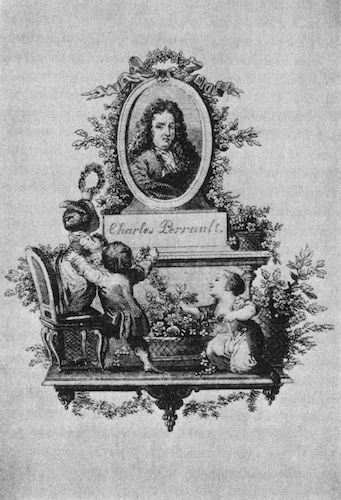
\includegraphics{image2.jpg}
\end{center}

\begin{otherlanguage}{french}

\clearpage
\thispagestyle{empty}
\addcontentsline{toc}{part}{HISTOIRES OU CONTES DU TEMPS PASSÉ (1697)}

\begin{center}
    \vspace*{3cm}
    {\LARGE \textbf{HISTOIRES \\ OU \\ CONTES DU TEMPS PASSÉ}\par}
    \vspace{1cm}
    {\Large \itshape Avec des Moralitéz.\par}
    \vspace{2cm}
    A PARIS,\\
    Chez Claude Barbin, sur le\\
    second Peron de la Sainte-Chapelle,\\
    au Palais.
    \vspace{1.5cm}
    \emph{Avec Privilége de Sa Majesté.} \\
    \vspace{0.5cm}
    M.DC.XCVII.
\end{center}
\clearpage

\thispagestyle{plain}
\addcontentsline{toc}{chapter}{A Mademoiselle}
\section*{A Mademoiselle}
\notesection{A Mademoiselle}

\begin{itshape}
Mademoiselle,

On ne trouvera pas étrange qu'un Enfant ait pris plaisir à
composer les Contes de ce Recüeil, mais on s'étonnera qu'il ait
eu la hardiesse de vous les presenter. Cependant, Mademoiselle,
quelque disproportion qu'il y ait entre la simplicité de ces
Recits, \& les lumieres de vostre esprit, si on examine bien ces
Contes, on verra que je ne suis pas aussi blamable que je le
parois d'abord. Ils renferment tous une Morale trés-sensée,
\& qui se découvre plus ou moins, selon le degré de pénetration
de ceux qui les lisent; d'ailleurs comme rien ne marque tant
la vaste estenduë d'un esprit, que de pouvoir s'élever en
même-temps aux plus grandes choses, \& s'abaisser aux plus
petites; on ne sera point surpris que la même Princesse, à qui
la Nature \& l'éducation ont rendu familier ce qu'il y a de
plus élevé, ne dédaigne pas de prendre plaisir à de semblables
bagatelles. Il est vray que ces Contes donnent une image de ce
qui se passe dans les moindres Familles, où la loüable impatience
d'instruire les enfans, fait imaginer des Histoires dépourveuës
de raison, pour s'accommoder à ces mêmes enfans qui n'en ont
pas encore; mais à qui convient-il mieux de connoître comment
vivent les Peuples, qu'aux Personnes que le Ciel destine à
les conduire ? Le desir de cette connoissance à poussé des Heros,
\& même des Heros de vostre Race, jusque dans des huttes \& des
cabanes, pour y voir de prés \& par eux-mêmes ce qui s'y passoit
de plus particulier: Cette connoissance leur ayant paru necessaire
pour leur parfaite instruction. Quoi qu'il en soit, Mademoiselle,

\begin{verse}
Pouvois-je mieux choisir pour rendre vrai-semblable \\
Ce que la Fable à d'incroyable ? \\
Et jamais Fée, au tems jadis \\
Fit-elle à jeune Créature, \\
Plus de dons, \& de dons exquis, \\
Que vous en a fait la Nature.
\end{verse}

\begin{flushright}
Je suis avec un trés-profond respect, \\
MADEMOISELLE, \\
De Vôtre Altesse Royale, \\
Le trés-humble \& \\
trés-obéissant serviteur, \\
P. Darmancour.
\end{flushright}

\end{itshape}

\chapter{LA BELLE AU BOIS DORMANT}
\notechapter{LA BELLE AU BOIS DORMANT}

\section{CONTE.}
\notesection{CONTE.}

Il estoit une fois un Roi \& une Reine, qui estoient si faschez de
n\textquotesingle avoir point d\textquotesingle enfans, si faschez
qu\textquotesingle on ne sçauroit dire. Ils allerent à toutes les eaux
du monde, vœux, pelerinages, menuës devotions; tout fut mis en œuvre, \&
rien n\textquotesingle y faisoit: Enfin pourtant la Reine devint grosse,
\& accoucha d\textquotesingle une fille: on fit un beau Baptesme; on
donna pour Maraines à la petite \ul{Princesse} toutes les Fées
qu\textquotesingle on pust trouver dans le Pays, (il
s\textquotesingle en trouva sept,) afin que chacune
d\textquotesingle elles luy faisant un don, comme
c\textquotesingle estoit la coustume des Fées en ce temps-là, la
Princesse eust par ce moyen toutes les perfections imaginables. Aprés
les ceremonies du Baptesme toute la compagnie revint au Palais du Roi,
où il y avoit un grand festin pour les Fées. On mit devant chacune
d\textquotesingle elles un couvert magnifique, avec un estui
d\textquotesingle or massif, où il y avoit une cuillier, une fourchette,
\& un couteau de fin or, garni de diamans \& de rubis. Mais comme chacun
prenoit sa place à table, on vit entrer une vieille Fée
qu\textquotesingle on n\textquotesingle avoit point priée parce
qu\textquotesingle il y avoit plus de cinquante ans
qu\textquotesingle elle n\textquotesingle estoit sortie
d\textquotesingle une Tour, \& qu\textquotesingle on la croyoit morte,
ou enchantée. Le Roi lui fit donner un couvert, mais il
n\textquotesingle y eut pas moyen de lui donner un estuy
d\textquotesingle or massif, comme aux autres, parce que
l\textquotesingle on n\textquotesingle en avoit fait faire que sept pour
les sept Fées. La vieille crût qu\textquotesingle on la méprisoit, \&
grommela quelques menaces entre ses dents: Une des jeunes Fées qui se
trouva auprés d\textquotesingle elle, l\textquotesingle entendit, \&
jugeant qu\textquotesingle elle pourrait donner quelque fâcheux don à la
petite Princesse, alla dés qu\textquotesingle on fut sorti de table, se
cacher derriere la tapisserie, afin de parler la derniere, \& de pouvoir
réparer autant qu\textquotesingle il luy seroit possible le mal que la
vieille auroit fait. Cependant les Fées commencerent à faire leurs dons
à la Princesse. La plus jeune luy donna pour don qu\textquotesingle elle
seroit la plus belle personne du monde, celle d\textquotesingle aprés
qu\textquotesingle elle auroit de l\textquotesingle esprit comme un
Ange, la troisiéme qu\textquotesingle elle auroit une grace admirable à
tout ce qu\textquotesingle elle feroit, la quatriéme
qu\textquotesingle elle danseroit parfaitement bien, la cinquiéme
qu\textquotesingle elle chanteroit comme un Rossignol, \& la sixiéme
qu\textquotesingle elle joüeroit de toutes sortes
d\textquotesingle instrumens dans la derniere perfection. Le rang de la
vieille Fée estant venu, elle dit en branlant la teste, encore plus de
dépit que de vieillesse, que la Princesse se perceroit la main
d\textquotesingle un fuseau, \& qu\textquotesingle elle en mourroit. Ce
terrible don fit fremir toute la compagnie, \& il n\textquotesingle y
eut personne qui ne pleurât. Dans ce moment la jeune Fée sortit de
derriere la tapisserie, \& dit tout haut ces paroles: Rassurez-vous Roi
et Reine, vostre fille n\textquotesingle en mourra pas: il est vrai que
je n\textquotesingle ay pas assez de puissance pour défaire entierement
ce que mon ancienne a fait. La Princesse se percera la main
d\textquotesingle un fuseau; mais au lieu d\textquotesingle en mourir,
elle tombera seulement dans un profond sommeil qui durera cent ans, au
bout desquels le fils d\textquotesingle un Roi viendra la réveiller. Le
Roi pour tâcher d\textquotesingle éviter le malheur annoncé par la
vieille, fit publier aussi tost un Edit, par lequel il deffendoit à
toutes personnes de filer au fuseau, ny d\textquotesingle avoir des
fuseaux chez soy sur peine de la vie. Au bout de quinze ou seize ans, le
Roi \& la Reine estant allez à une de leurs Maisons de plaisance, il
arriva que la jeune Princesse courant un jour dans le Château, \&
montant de chambre en chambre, alla jusqu\textquotesingle au haut
d\textquotesingle un donjon dans un petit galletas, où une bonne Vieille
estoit seule à filer sa quenoüille. Cette bonne femme
n\textquotesingle avoit point ouï parler des deffenses que le Roi avoit
faites de filer au fuseau. Que faites-vous-là, ma bonne femme, dit la
Princesse; je file, ma belle enfant, luy répondit la vieille qui ne la
connoissoit pas. Ha! que cela est joli, reprit la Princesse, comment
faites-vous? donnez-moy que je voye si j\textquotesingle en ferois bien
autant. Elle n\textquotesingle eust pas plutost pris le fuseau, que
comme elle estoit fort vive, un peu estourdie, \& que
d\textquotesingle ailleurs l\textquotesingle Arrest des Fées
l\textquotesingle ordonnoit ainsi, elle s\textquotesingle en perça la
main, \& tomba évanouie. La bonne vieille bien embarrassée, crie au
secours: on vient de tous costez, on jette de l\textquotesingle eau au
visage de la Princesse, on la délasse, on luy frappe dans les mains, on
luy frotte les temples avec de l\textquotesingle eau de la Reine de
Hongrie; mais rien ne la faisoit revenir. Alors le Roy, qui estoit monté
au bruit, se souvint de la prédiction des Fées, \& jugeant bien
qu\textquotesingle il falloit que cela arrivast, puisque les Fées
l\textquotesingle avoient dit, fit mettre la Princesse dans le plus bel
appartement du Palais, sur un lit en broderie d\textquotesingle or \&
d\textquotesingle argent; on eut dit d\textquotesingle un Ange, tant
elle estoit belle; car son évanoüissement n\textquotesingle avoit pas
osté les couleurs vives de son teint: ses jouës estoient incarnates, \&
ses lévres comme du corail: elle avoit seulement les yeux fermez, mais
on l\textquotesingle entendoit respirer doucement, ce qui faisoit voir
qu\textquotesingle elle n\textquotesingle estoit pas morte. Le Roi
ordonna qu\textquotesingle on la laissast dormir en repos,
jusqu\textquotesingle à ce que son heure de se réveiller fust venuë. La
bonne Fée qui luy avoit sauvé la vie, en la condamnant à dormir cent
ans, estoit dans le Royaume de Mataquin, à douze mille lieuës de là
lorsque l\textquotesingle accident arriva à la Princesse; mais elle en
fut avertie en un instant par un petit Nain, qui avoit des bottes de
sept lieuës, (c\textquotesingle estoit des bottes avec lesquelles on
faisoit sept lieuës d\textquotesingle une seule enjambée.) La Fée partit
aussi tost, \& on la vit au bout d\textquotesingle une heure arriver
dans un chariot tout de feu, traisné par des dragons. Le Roi luy alla
presenter la main à la descente du chariot. Elle approuva tout ce
qu\textquotesingle il avoit fait; mais comme elle estoit grandement
prévoyante, elle pensa que quand la Princesse viendroit à se réveiller,
elle seroit bien embarassée toute seule dans ce vieux Château: voicy ce
qu\textquotesingle elle fit. Elle toucha de sa baguette tout ce qui
estoit dans ce Chasteau, (hors le Roi \& la Reine) Gouvernantes,
Filles-d\textquotesingle Honneur, Femmes-de-Chambre, Gentilshommes,
Officiers, Maistrés-d\textquotesingle Hostel, Cuisiniers, Marmitons,
Galopins, Gardes, Suisses, Pages, Valets-de-pied; elle toucha aussi tous
les chevaux qui estoient dans les Ecuries, avec les Palfreniers, les
gros mâtins de basse cour, \& la petite Pouffe, petite chienne de la
Princesse, qui estoit auprés d\textquotesingle elle sur son lit. Dés
qu\textquotesingle elle les eust touchez, ils
s\textquotesingle endormirent tous, pour ne se réveiller
qu\textquotesingle en même temps que leur Maistresse, afin
d\textquotesingle estre tout prests à la servir quand elle en auroit
besoin: les broches mêmes qui estoient au feu toutes pleines de perdrix
\& de faizans s\textquotesingle endormirent, \& le feu aussi. Tout cela
se fit en un moment; les Fées n\textquotesingle estoient pas longues à
leur besogne. Alors le Roi \& la Reine aprés avoir baisé leur chere
enfant sans qu\textquotesingle elle s\textquotesingle éveillast,
sortirent du Chasteau, \& firent publier des deffenses à qui que ce soit
d\textquotesingle en approcher. Ces \ul{deffenses}
n\textquotesingle estoient pas necessaires, car il crut dans un
quart-d\textquotesingle heure tout au tour du parc une si grande
quantité de grands arbres \& de petits, de ronces \&
d\textquotesingle épines entrelassées les unes dans les autres, que
beste ny homme n\textquotesingle y auroit pû passer: en sorte
qu\textquotesingle on ne voyoit plus que le haut des Tours du Chasteau,
encore n\textquotesingle estoit-ce que de bien loin. On ne douta point
que la Fée n\textquotesingle eust encore fait là un tour de son metier,
afin que la Princesse pendant qu\textquotesingle elle dormiroit,
n\textquotesingle eust rien à craindre des Curieux.

Au bout de cent ans, le Fils du Roi qui regnoit alors, \& qui estoit
d\textquotesingle une autre famille que la Princesse endormie, estant
allé à la chasse de ce costé-là, demanda ce que c\textquotesingle estoit
que des Tours qu\textquotesingle il voyoit au dessus
d\textquotesingle un grand bois fort épais, chacun luy répondit selon
qu\textquotesingle il en avoit ouï parler. Les uns disoient que
c\textquotesingle estoit un vieux Château où il revenoit des Esprits;
les autres que tous les Sorciers de la contrée y faisoient leur sabbat.
La plus commune opinion estoit qu\textquotesingle un Ogre y demeuroit,
\& que là il emportoit tous les enfans qu\textquotesingle il pouvoit
attraper, pour les pouvoir manger à son aise, \& sans
qu\textquotesingle on le pust suivre, ayant seul le pouvoir de se faire
un passage au travers du bois. Le Prince ne sçavoit
qu\textquotesingle en croire, lors qu\textquotesingle un vieux Paysan
prit la parole, \& luy dit: Mon Prince, il y a plus de cinquante ans que
j\textquotesingle ay ouï dire à mon pere, qu\textquotesingle il y avoit
dans ce Chasteau une Princesse, la plus belle du monde;
qu\textquotesingle elle y devoit dormir cent ans, \&
qu\textquotesingle elle seroit reveillée par le fils
d\textquotesingle un Roy, à qui elle estoit reservée. Le jeune Prince à
ce discours se sentit tout de feu; il crut sans balancer
qu\textquotesingle il mettroit fin à une si belle avanture, \& poussé
par l\textquotesingle amour \& par la gloire, il résolut de voir sur le
champ ce qui en estoit. A peine s\textquotesingle avança-t-il vers le
bois, que tous ces grands arbres, ces ronces \& ces épines
s\textquotesingle écarterent d\textquotesingle elles-mesmes pour le
laisser passer: il marche vers le Chasteau qu\textquotesingle il voyoit
au bout d\textquotesingle une grande avenuë où il entra, \& ce qui le
surprit un peu, il vit que personne de ses gens ne
l\textquotesingle avoient pû suivre, parce que les arbres
s\textquotesingle estoient rapprochez dés qu\textquotesingle il avoit
esté passé. Il ne laissa pas de continuer son chemin: un Prince jeune \&
amoureux est toûjours vaillant. Il entra dans une grande avancour où
tout ce qu\textquotesingle il vit d\textquotesingle abord estoit capable
de le glacer de crainte: c\textquotesingle estoit un silence affreux,
l\textquotesingle image de la mort s\textquotesingle y presentoit par
tout, \& ce n\textquotesingle estoit que des corps étendus
d\textquotesingle hommes \& d\textquotesingle animaux, qui paroissoient
morts. Il reconnut pourtant bien au nez bourgeonne, \& à la face
vermeille des Suisses, qu\textquotesingle ils n\textquotesingle estoient
qu\textquotesingle endormis, \& leur tasses où il y avoit encore
quelques goutes de vin, montroient assez qu\textquotesingle ils
s\textquotesingle estoient endormis en beuvant. Il passe une grande cour
pavée de marbre, il monte l\textquotesingle escalier, il entre dans la
salle des Gardes qui estoient rangez en haye, la carabine sur
l\textquotesingle épaule, \& ronflans de leur mieux. Il traverse
plusieurs chambres pleines de Gentilshommes \& de Dames, dormans tous,
les uns de bout, les autres assis; il entre dans une chambre toute
dorée, \& il vit sur un lit, dont les rideaux éstoient ouverts de tous
côtez, le plus beau spectacle qu\textquotesingle il eut jamais veu: Une
Princesse qui paroissoit avoir quinze ou seize ans, \& dont
l\textquotesingle éclat resplendissant avoit quelque chose de lumineux
\& de divin. Il s\textquotesingle approcha en tremblant \& en admirant,
\& se mit à genoux auprés d\textquotesingle elle. Alors comme la fin de
l\textquotesingle enchantement estoit venuë, la Princesse
s\textquotesingle éveilla; \& le regardant avec des yeux plus tendres
qu\textquotesingle une premiere veuë ne sembloit le permettre; est-ce
vous, mon Prince, luy dit-elle, vous vous estes bien fait attendre. Le
Prince charmé de ces paroles, \& plus encore de la maniere dont elles
estoient dites, ne sçavoit comment luy temoigner sa joye \& sa
reconnoissance; il l\textquotesingle assura qu\textquotesingle il
l\textquotesingle aimoit plus que luy-mesme. Ses discours furent mal
rangez, ils en plûrent davantage, peu d\textquotesingle éloquence,
beaucoup d\textquotesingle amour: Il estoit plus embarassé
qu\textquotesingle elle, \& l\textquotesingle on ne doit pas
s\textquotesingle en estonner; elle avoit eu le temps de songer à ce
qu\textquotesingle elle auroit à luy dire; car il y a apparence,
(l\textquotesingle Histoire n\textquotesingle en dit pourtant rien) que
la bonne Fée pendant un si long sommeil, luy avoit procuré le plaisir
des songes agreables. Enfin il y avoit quatre heures
qu\textquotesingle ils se parloient, \& ils ne s\textquotesingle étoient
pas encore dit la moitié des choses qu\textquotesingle ils avoient à se
dire.

Cependant tout le Palais s\textquotesingle estoit réveillé avec la
Princesse; chacun songeoit à faire sa charge, \& comme ils
n\textquotesingle estoient pas tous amoureux, ils mouroient de faim; la
Dame d\textquotesingle honneur pressée comme les autres,
s\textquotesingle impatienta, \& dit tout haut à la Princesse que la
viande estoit servie. Le Prince aida à la Princesse à se lever; elle
estoit tout habillée \& fort magnifiquement; mais il se garda bien de
luy dire qu\textquotesingle elle estoit habillée comme ma mere grand, \&
qu\textquotesingle elle avoit un collet monté, elle n\textquotesingle en
estoit pas moins belle. Ils passerent dans un Salon de miroirs, \& y
souperent, servis par les Officiers de la Princesse; les Violons \& les
Hautbois joüerent de vieilles pieces, mais excellentes, quoy
qu\textquotesingle il y eut prés de cent ans qu\textquotesingle on ne
les joüast plus; \& aprés soupé sans perdre de temps, le grand Aumonier
les maria dans la Chapelle du Chateau, \& la
Dame-d\textquotesingle honneur leur tira le rideau; ils dormirent peu,
la Princesse n\textquotesingle en avoit pas grand besoin, \& le Prince
la quitta dés le matin pour retourner à la Ville, où son Pere devoit
estre en peine de luy: le Prince luy dit, qu\textquotesingle en chassant
il s\textquotesingle estoit perdu dans la forest, \&
qu\textquotesingle il avoit couché dans la hutte d\textquotesingle un
Charbonnier, qui luy avoit fait manger du pain noir \& du fromage. Le
Roi son pere qui estoit bon-homme, le crut, mais sa Mere
n\textquotesingle en fut pas bien persuadée, \& voyant
qu\textquotesingle il alloit presque tous les jours à la chasse, \&
qu\textquotesingle il avoit toûjours une raison en main pour
s\textquotesingle excuser, quand il avoit couché deux ou trois nuits
dehors, elle ne douta plus qu\textquotesingle il n\textquotesingle eut
quelque amourette: car il vêcut avec la Princesse plus de deux ans
entiers, \& en eut deux enfans, dont le premier qui fut une fille, fut
nommée l\textquotesingle Aurore, \& le second un fils,
qu\textquotesingle on nomma le Jour, parce qu\textquotesingle il
paroissoit encore plus beau que sa sœur. La Reine dit plusieurs fois à
son fils, pour le faire expliquer, qu\textquotesingle il falloit se
contenter dans la vie, mais il n\textquotesingle osa jamais se fier à
elle de son secret; il la craignoit quoy qu\textquotesingle il
l\textquotesingle aimast, car elle estoit de race Ogresse, \& le Roi ne
l\textquotesingle avoit épousée qu\textquotesingle à cause de ses grands
biens; on disoit même tout bas à la Cour qu\textquotesingle elle avoit
les inclinations des Ogres, \& qu\textquotesingle en voyant passer de
petits enfans, elle avoit toutes les peines du monde à se retenir de se
jetter sur eux; ainsi le Prince ne voulut jamais rien dire. Mais quand
le Roy fut mort, ce qui arriva au bout de deux ans, \&
qu\textquotesingle il se vit le maistre, il declara publiquement son
Mariage, \& alla en grande ceremonie querir la Reine sa femme dans son
Chasteau. On luy fit une entrée magnifique dans la Ville Capitale, où
elle entra au milieu de ces deux enfans. Quelque temps aprés le Roi alla
faire la guerre à l\textquotesingle Empereur Cantalabutte son voisin. Il
laissa la Regence du Royaume à la Reine sa mere, \& luy recommanda fort
sa femme \& ses enfans: il devoit estre à la guerre tout
l\textquotesingle Esté, \& dés qu\textquotesingle il fut parti, la
Reine-Mere envoya sa Bru \& ses enfans à une maison de campagne dans les
bois, pour pouvoir plus aisément assouvir son horrible envie. Elle y
alla quelques jours aprés, \& dit un soir à son Maistre
d\textquotesingle Hôtel, je veux manger demain à mon dîner la petite
Aurore. Ah! Madame, dit le Maistre d\textquotesingle Hôtel; je le veux,
dit la Reine (\& elle le dit d\textquotesingle un ton
d\textquotesingle Ogresse, qui a envie de manger de la chair fraische)
\& je la veux manger à la Sausse-robert. Ce pauvre homme voyant bien
qu\textquotesingle il ne falloit pas se joüer à une Ogresse, prit son
grand cousteau, \& monta à la chambre de la petite Aurore: elle avoit
pour lors quatre ans, \& vint en sautant \& en riant se jetter à son
col, \& luy demander du bon du bon. Il se mit à pleurer, le couteau luy
tomba des mains, \& il alla dans la basse-cour couper la gorge à un
petit agneau, et luy fit une si bonne sausse, que sa Maîtresse
l\textquotesingle assura qu\textquotesingle elle n\textquotesingle avoit
jamais rien mangé de si bon. Il avoit emporté en même temps la petite
Aurore, \& l\textquotesingle avoit donnée à sa femme pour la cacher,
dans le logement qu\textquotesingle elle avoit au fond de la basse-cour.
Huit jours aprés la méchante Reine dit à son
Maistre-d\textquotesingle Hôtel, je veux manger à mon souper le petit
Jour: il ne repliqua pas, résolu de la tromper comme
l\textquotesingle autre fois; il alla chercher le petit Jour, \& le
trouva avec un petit fleuret à la main, dont il faisoit des armes avec
un gros Singe, il n\textquotesingle avoit pourtant que trois ans: il le
porta à sa femme qui le cacha avec la petite Aurore, \& donna à la place
du petit Jour, un petit chevreau fort tendre, que
l\textquotesingle Ogresse trouva admirablement bon.

Cela estoit fort bien allé jusques-là, mais un soir cette méchante Reine
dit au Maistre-d\textquotesingle Hôtel, je veux manger la Reine à la
mesme sausse que ses enfans. Ce fut alors que le pauvre
Maistre-d\textquotesingle Hôtel desespera de la pouvoir encore tromper.
La jeune Reine avoit vingt ans passez, sans compter les cent ans
qu\textquotesingle elle avoit dormi: sa peau estoit un peu dure, quoyque
belle \& blanche; \& le moyen de trouver dans la Ménagerie une beste
aussi dure que cela: il prit la résolution pour sauver sa vie, de couper
la gorge à la Reine, \& monta dans sa chambre, dans
l\textquotesingle intention de n\textquotesingle en pas faire à deux
fois; il s\textquotesingle excitoit à la fureur, \& il entra le poignard
à la main dans la chambre de la jeune Reine: Il ne voulut pourtant point
la surprendre, \& il lui dit avec beaucoup de respect,
l\textquotesingle ordre qu\textquotesingle il avoit receu de la
Reine-Mere. Faites vostre devoir, luy dit-elle, en lui tendant le col;
executez l\textquotesingle ordre qu\textquotesingle on vous a donné;
j\textquotesingle irai revoir mes enfans, mes pauvres enfans que
j\textquotesingle ay tant aimez, car elle les croyoit morts depuis
qu\textquotesingle on les avoit enlevez sans lui rien dire. Non, non,
Madame, lui répondit le pauvre Maistre-d\textquotesingle Hôtel tout
attendri, vous ne mourrez point, \& vous ne laisserez pas
d\textquotesingle aller revoir vos chers enfans, mais ce sera chez moy
où je les ay cachez, \& je tromperay encore la Reine, en luy faisant
manger une jeune biche en vostre place. Il la mena aussi-tost à sa
chambre, où la laissant embrasser ses enfans \& pleurer avec eux: il
alla accommoder une biche, que la Reine mangea à son soupé, avec le même
appetit que si c\textquotesingle eut esté la jeune Reine. Elle estoit
bien contente de sa cruauté, \& elle se préparoit à dire au Roy à son
retour, que les loups enragez avoient mangé la Reine sa femme \& ses
deux enfans.

Un soir qu\textquotesingle elle rodoit à son ordinaire dans les cours \&
basse-cours du Chasteau pour y halener quelque viande fraische, elle
entendit dans une sale basse le petit Jour qui pleuroit, parce que la
Reine sa mere le vouloit faire foüetter, à cause qu\textquotesingle il
avoit esté méchant, \& elle entendit aussi la petite Aurore qui
demandoit pardon pour son frere. L\textquotesingle Ogresse reconnut la
voix de la Reine \& de ses enfans, \& furieuse d\textquotesingle avoir
esté trompée, elle commande dés le lendemain au matin, avec une voix
épouventable, qui faisoit trembler tout le monde, qu\textquotesingle on
apportast au milieu de la cour une grande cuve, qu\textquotesingle elle
fit remplir de crapaux, de viperes, de couleuvres \& de serpens, pour y
faire jetter la Reine, \& ses enfans, le
Maistre-d\textquotesingle Hôstel, sa femme \& sa servante: elle avoit
donné ordre de les amener les mains liées derriere le dos. Ils estoient
là, \& les bourreaux se preparoient à les jetter dans la cuve, lorsque
le Roi qu\textquotesingle on n\textquotesingle attendoit pas si tost,
entra dans la cour à cheval; il estoit venu en poste, \& demanda tout
estonné ce que vouloit dire cet horrible spectacle; personne
n\textquotesingle osoit l\textquotesingle en instruire, quand
l\textquotesingle Ogresse, enragée de voir ce quelle voyoit, se jetta
elle-mesme la teste la premiere dans la cuve, \& fût devorée en un
instant par les vilaines bestes qu\textquotesingle elle y avoit fait
mettre. Le Roi ne laissa pas d\textquotesingle en estre fasché, elle
estoit sa mere, mais il s\textquotesingle en consola bientost avec sa
belle femme \& ses enfans. \\

\section{MORALITÉ.}
\notesection{MORALITÉ.}

\begin{verse}
  \small
Attendre quelque temps pour avoir un Epoux, \\
Riche bien-fait, galant \& doux,\\
La chose est assez naturelle, \\
Mais l\textquotesingle attendre cent ans et toûjours en dormant,  \\
 On ne trouve plus de femelle, \\
Qui dormist si tranquillement. \\
La Fable semble encor vouloir nous faire entendre, \\
Que souvent de l\textquotesingle Hymen les agreables nœuds,  \\
Pour estre differez n\textquotesingle en sont pas moins heureux,  \\
Et qu\textquotesingle on ne perd rien pour attendre; \\
Mais le sexe avec tant d\textquotesingle ardeur, \\
Aspire à la foy conjugale, \\
Que je n\textquotesingle ay pas la force ny le cœur, \\
De luy prescher cette Morale.
\end{verse}

\chapter{LE PETIT CHAPERON ROUGE}
\notechapter{LE PETIT CHAPERON ROUGE}

\section{CONTE.}
\notesection{CONTE.}

Il estoit une fois une petite fille de Village, la plus jolie
qu\textquotesingle on eut sçû voir; sa mere en estoit folle, \& sa mere
grand plus folle encore. Cette bonne femme luy fit faire un petit
chaperon rouge, qui luy seïoit si bien, que par tout on
l\textquotesingle appelloit le Petit chaperon rouge.

Un jour sa mere ayant cui \& fait des galettes, luy dit, va voir comme
se porte ta mere-grand, car on m\textquotesingle a dit
qu\textquotesingle elle estoit malade, porte luy une galette \& ce petit
pot de beure. Le petit chaperon rouge partit aussi-tost pour aller chez
sa mere-grand, qui demeuroit dans un autre Village. En passant dans un
bois elle rencontra compere le Loup, qui eut bien envie de la manger,
mais il n\textquotesingle osa, à cause de quelques Bucherons qui
estoient dans la Forest. Il luy demanda où elle alloit; la pauvre enfant
qui ne sçavoit pas qu\textquotesingle il est dangereux de
s\textquotesingle arrester à écouter un Loup, luy dit, je vais voir ma
Mere-grand, \& luy porter une galette avec un petit pot de beurre, que
ma Mere luy envoye. Demeure-t\textquotesingle elle bien loin, lui dit le
Loup? Oh ouy, dit le petit chaperon rouge, c\textquotesingle est par
de-là le moulin que vous voyez tout là-bas, là-bas, à la premiere maison
du Village. Et bien, dit le Loup, je veux l\textquotesingle aller voir
aussi; je m\textquotesingle y en vais par ce chemin icy, \& toi par ce
chemin-là, \& nous verrons qui plûtost y sera. Le Loup se mit à courir
de toute sa force par le chemin qui estoit le plus court, \& la petite
fille s\textquotesingle en alla par le chemin le plus long,
s\textquotesingle amusant à cueillir des noisettes, à courir aprés des
papillons, \& à faire des bouquets des petites fleurs
qu\textquotesingle elle rencontroit. Le Loup ne fut pas long-temps à
arriver à la maison de la Mere-grand, il heurte: Toc, toc, qui est-là?
C\textquotesingle est vôtre fille le petit chaperon rouge (dit le Loup,
en contrefaisant sa voix) qui vous apporte une galette, \& un petit pot
de beurre que ma Mere vous envoye. La bonne Mere-grand qui estoit dans
son lit à cause qu\textquotesingle elle se trouvoit un peu mal, luy
cria, tire la \ul{chevillette}, la bobinette chera, le Loup tira la
chevillette, \& la porte s\textquotesingle ouvrit. Il se jetta sur la
bonne femme, \& la devora en moins de rien; car il y avoit plus de trois
jours qu\textquotesingle il n\textquotesingle avoit mangé. Ensuite il
ferma la porte, \& s\textquotesingle alla coucher dans le lit de la
Mere-grand, en attendant le petit chaperon rouge, qui quelque temps
aprés vint heurter à la porte. Toc, toc: qui est là? Le petit chaperon
rouge qui entendit la grosse voix du Loup, eut peur
d\textquotesingle abord, mais croyant que sa Mere-grand estoit enrhumée,
répondit, c\textquotesingle est vostre fille le petit chaperon rouge,
qui vous apporte une galette \& un petit pot de beurre que ma Mere vous
envoye. Le Loup luy cria, en adoucissant un peu sa voix; tire la
chevillette, la bobinette chera. Le petit chaperon rouge tira la
chevillette, \& la porte s\textquotesingle ouvrit. Le Loup la voyant
entrer, lui dit en se cachant dans le lit sous la couverture: mets la
galette \& le petit pot de beurre sur la huche, \& viens te coucher avec
moy. Le petit chaperon rouge se deshabille, \& va se mettre dans le lit,
où elle fut bien estonnée de voir comment sa Mere-grand estoit faite en
son deshabillé, elle luy dit, ma mere-grand que vous avez de grands
bras! c\textquotesingle est pour mieux t\textquotesingle embrasser, ma
fille: ma mere-grand que vous avez de grandes jambes?
c\textquotesingle est pour mieux courir mon enfant: ma mere-grand que
vous avez de grandes oreilles? c\textquotesingle est pour mieux écouter
mon enfant. Ma mere-grand que vous avez de grands yeux?
c\textquotesingle est pour mieux voir, mon enfant. Ma mere-grand que
vous avez de grandes dens? c\textquotesingle est pour te manger. Et en
disant ces mots, ce méchant Loup se jetta sur le petit chaperon rouge,
\& la mangea. \\

\section{MORALITÉ.}
\notesection{MORALITÉ.}

\begin{verse}
  \small
On voit icy que de jeunes enfans, \\
Sur tout de jeunes filles, \\
Belles, bien faites, \& gentilles, \\
Font tres-mal d\textquotesingle écouter toute sorte de gens, \\
Et que ce n\textquotesingle est pas chose étrange, \\
S\textquotesingle il en est tant que le loup mange. \\
Je dis le loup, car tous les loups; \\
Ne sont pas de la mesme sorte; \\
Il en est d\textquotesingle une humeur accorte, \\
Sans bruit, sans fiel \& sans couroux, \\
Qui privez, complaisans \& doux, \\
Suivant les jeunes Demoiselles, \\
Jusque dans les maisons, jusque dans les ruelles;  \\
Mais helas! qui ne sçait que ces Loups doucereux,  \\
De tous les Loups sont les plus dangereux.
\end{verse}

\chapter{LA BARBE BLEUË.}
\notechapter{LA BARBE BLEUË.}

\section{CONTE.}
\notesection{CONTE.}

Il estoit une fois un homme qui avoit de belles maisons à la Ville \& à
la Campagne, de la vaisselle d\textquotesingle or \&
d\textquotesingle argent, des meubles en broderie, \& des carosses tout
dorez; mais par malheur cet homme avoit la Barbe-bleüe: cela le rendoit
si laid \& si terrible, qu\textquotesingle il n\textquotesingle estoit
ni femme ni fille qui ne s\textquotesingle enfuit de devant luy. Une de
ses Voisines, Dame de qualité avoit deux filles parfaitement belles. Il
luy en demanda une en Mariage, \& luy laissa le choix de celle
qu\textquotesingle elle voudroit luy donner. Elles n\textquotesingle en
vouloient point toutes deux, \& se le renvoyoient l\textquotesingle une
à l\textquotesingle autre, ne pouvant se resoudre à prendre un homme qui
eut la barbe bleüe. Ce qui les degoûtoit encore, c\textquotesingle est
qu\textquotesingle il avoit déja épousé plusieurs femmes, \&
qu\textquotesingle on ne sçavoit ce que ces femmes estoient devenuës. La
Barbe bleuë pour faire connoissance, les mena avec leur Mere, \& trois
ou quatre de leurs meilleures amies, \& quelques jeunes gens du
voisinage, à une de ses maisons de Campagne, où on demeura huit jours
entiers. Ce n\textquotesingle estoit que promenades, que parties de
chasse \& de pesche, que danses \& festins, que collations: on ne
dormoit point, \& on passoit toute la nuit à se faire des malices les
uns aux autres: enfin tout alla si bien, que la Cadette commença à
trouver que le Maistre du logis n\textquotesingle avoit plus la barbe si
bleüe, \& que c\textquotesingle estoit un fort honneste homme. Dés
qu\textquotesingle on fust de retour à la Ville, le Mariage se conclut.
Au bout d\textquotesingle un mois la Barbe bleüe dit à sa femme
qu\textquotesingle il estoit obligé de faire un voyage en Province, de
six semaines au moins, pour une affaire de consequence;
qu\textquotesingle il la prioit de se bien divertir pendant son absence,
qu\textquotesingle elle fit venir ses bonnes amies,
qu\textquotesingle elle les menast à la Campagne si elle vouloit, que
par tout elle fit bonne chere: Voila, luy dit-il, les clefs des deux
grands garde-meubles, voilà celles de la vaisselle d\textquotesingle or
\& d\textquotesingle argent qui ne sert pas tous les jours, voilà celles
de mes coffres forts, où est mon or \& mon argent, celles des cassettes
où sont mes pierreries, \& voilà le passe-par-tout de tous les
appartemens: pour cette petite clef-cy, c\textquotesingle est la clef du
cabinet au bout de la grande gallerie de l\textquotesingle appartement
bas: ouvrez tout, allez par tout, mais pour ce petit cabinet je vous
deffens d\textquotesingle y entrer, \& je vous le deffens de telle
sorte, que s\textquotesingle il vous arrive de l\textquotesingle ouvrir,
il n\textquotesingle y a rien que vous ne deviez attendre de ma colere.
Elle promit d\textquotesingle observer exactement tout ce qui luy venoit
d\textquotesingle estre ordonné: \& luy, aprés l\textquotesingle avoir
embrassée, il monte dans son carosse, \& part pour son voyage. Les
voisines \& les bonnes amies n\textquotesingle attendirent pas
qu\textquotesingle on les envoyast querir pour aller chez la jeune
Mariée, tant elles avoient d\textquotesingle impatience de voir toutes
les richesses de sa Maison, n\textquotesingle ayant osé y venir pendant
que le Mari y estoit, à cause de sa Barbe bleuë qui leur faisoit peur.
Les voilà aussi-tost à parcourir les chambres, les cabinets, les
garderobes, toutes plus belles \& plus riches les unes que les autres.
Elles monterent en suite aux gardemeubles, où elles ne pouvoient assez
admirer le nombre \& la beauté des tapisseries, des lits, des sophas,
des cabinets, des gueridons, des tables \& des miroirs, où
l\textquotesingle on se voyoit depuis les pieds jusqu\textquotesingle à
la teste, \& dont les bordures les unes de glace, les autres
d\textquotesingle argent, \& de vermeil doré, estoient les plus belles
\& les plus magnifiques qu\textquotesingle on eut jamais veuës: Elles ne
cessoient d\textquotesingle exagerer \& d\textquotesingle envier le bon
heur de leur amie, qui cependant ne se divertissoit point à voir toutes
ces richesses, à cause de l\textquotesingle impatience
qu\textquotesingle elle avoit d\textquotesingle aller ouvrir le cabinet
de l\textquotesingle appartement bas. Elle fut si pressée de sa
curiosité, que sans considerer qu\textquotesingle il estoit malhonneste
de quitter sa compagnie, elle y descendit par un petit escalier dérobé,
\& avec tant de precipitation, qu\textquotesingle elle pensa se rompre
le cou deux ou trois fois. Estant arrivée à la porte du cabinet, elle
s\textquotesingle y arresta quelque temps, songeant à la deffense que
son Mari luy avoit faite, \& considerant qu\textquotesingle il pourrait
luy arriver malheur d\textquotesingle avoir esté desobeïssante; mais la
tentation estoit si forte qu\textquotesingle elle ne put la surmonter:
elle prit donc la petite clef, \& ouvrit en tremblant la porte du
cabinet. D\textquotesingle abord elle ne vit rien, parce que les
fenestres estoient fermées; aprés quelques momens elle commença à voir
que le plancher estoit tout couvert de sang caillé, \& que dans ce sang
se miroient les corps de plusieurs femmes mortes, \& attachées le long
des murs. (C\textquotesingle étoit toutes les femmes que la Barbe bleuë
avoit épousées \& qu\textquotesingle il avoit égorgées
l\textquotesingle une aprés l\textquotesingle autre.) Elle pensa mourir
de peur, \& la clef du cabinet qu\textquotesingle elle venoit de retirer
de la serrure luy tomba de la main: aprés avoir un peu repris ses
esprits, elle ramassa la clef, referma la porte, \& monta à sa chambre
pour se remettre un peu, mais elle n\textquotesingle en pouvoit venir à
bout, tant elle estoit émeuë. Ayant remarqué que la clef du cabinet
étoit tachée de sang, elle l\textquotesingle essuia deux ou trois fois,
mais le sang ne s\textquotesingle en alloit point; elle eut beau la
laver, \& mesme la frotter avec du sablon \& avec du grais, il demeura
toûjours du sang, car la clef estait Fée, \& il n\textquotesingle y
avoit pas moyen de la nettoyer tout-à-fait: quand on ôtoit le sang
d\textquotesingle un costé, il revenoit de l\textquotesingle autre. La
Barbe-bleuë revint de son voyage dés le soir mesme, \& dit
qu\textquotesingle il avoit reçeu des Lettres dans le chemin, qui luy
avoient appris que l\textquotesingle affaire pour laquelle il estoit
party, venoit d\textquotesingle estre terminée à son avantage. Sa femme
fit tout ce qu\textquotesingle elle pût pour luy témoigner
qu\textquotesingle elle estoit ravie de son promt retour. Le lendemain
il luy redemanda les clefs, \& elle les luy donna, mais
d\textquotesingle une main si tremblante, qu\textquotesingle il devina
sans peine tout ce qui s\textquotesingle estoit passé.
D\textquotesingle où vient, luy dit-il, que la clef du cabinet
n\textquotesingle est point avec les autres: il faut, dit-elle, que je
l\textquotesingle aye laissée là-haut sur ma table. Ne manquez pas, dit
la Barbe bleuë de me la donner tantost; aprés plusieurs remises il falut
apporter la clef. La Barbe bleuë l\textquotesingle ayant considerée, dit
à sa femme, pourquoy y a-t-il du sang sur cette clef? je
n\textquotesingle en sçais rien, répondit la pauvre femme, plus pasle
que la mort: Vous n\textquotesingle en sçavez rien, reprit la Barbe
bleuë, je le sçay bien moy, vous avez voulu entrer dans le cabinet? Hé
bien, Madame, vous y entrerez, \& irez prendre vostre place auprés des
Dames que vous y avez veuës. Elle se jetta aux pieds de son Mari, en
pleurant et en luy demandant pardon, avec toutes les marques
d\textquotesingle un vrai repentir de n\textquotesingle avoir pas esté
obeissante. Elle auroit attendri un rocher, belle \& affligée comme elle
estoit; mais la Barbe bleuë avoit le cœur plus dur qu\textquotesingle un
rocher: Il faut mourir, Madame, luy dit-il, \& tout à
l\textquotesingle heure. Puis qu\textquotesingle il faut mourir,
répondit-elle, en le regardant, les yeux baignez de larmes, donnez moy
un peu de temps pour prier Dieu. Je vous donne un
demy-quart-d\textquotesingle heure, reprit la Barbe bleüe, mais pas un
moment davantage. Lors qu\textquotesingle elle fut seule, elle appella
sa sœur, \& luy dit, ma sœur Anne, car elle s\textquotesingle appelloit
ainsi, monte je te prie sur le haut de la Tour, pour voir si mes freres
ne viennent point, ils m\textquotesingle ont promis
qu\textquotesingle ils me viendroient voir aujourd\textquotesingle huy,
\& si tu les vois, fais-leur signe de se hâter. La sœur Anne monta sur
le haut de la Tour, \& la pauvre affligée luy crioit de temps en temps,
\emph{Anne, ma sœur Anne, ne vois-tu rien venir}. Et la sœur Anne luy
répondoit, \emph{je ne vois rien que le Soleil qui poudroye, \&
l\textquotesingle herbe qui verdoye}. Cependant la Barbe bleüe tenant un
grand coutelas à sa main, crioit de toute sa force à sa femme, descens
viste, ou je monteray là-haut. Encore un moment s\textquotesingle il
vous plaist, luy répondoit sa femme, \& aussi-tost elle crioit tout bas,
\emph{Anne, ma sœur Anne, ne vois-tu rien venir}, \& la sœur Anne
répondoit, \emph{je ne voy rien que le Soleil qui poudroye, \&
l\textquotesingle herbe qui verdoye}. Descens donc viste, crioit la
Barbe bleuë, ou je monteray là haut. Je m\textquotesingle en vais,
répondoit sa femme, \& puis elle crioit \emph{Anne, ma sœur Anne, ne
vois-tu rien venir}. Je vois, répondit la sœur Anne, une grosse
poussiere qui vient de ce costé-cy. Sont-ce mes freres? Helas, non, ma
sœur, c\textquotesingle est un Troupeau de Moutons. Ne veux-tu pas
descendre, crioit la Barbe bleuë. Encore un moment répondoit sa femme \&
puis elle crioit, \emph{Anne, ma sœur Anne, ne vois-tu rien venir}. Je
vois, répondit-elle, deux Cavaliers qui viennent de ce costé-cy, mais il
sont bien loin encore: Dieu soit loué,
s\textquotesingle écria-t\textquotesingle elle un moment aprés, ce sont
mes freres; je leur fais signe tant que je puis de se haster. La Barbe
bleüe se mit à crier si fort que toute la maison en trembla. La pauvre
femme descendit, \& alla se jetter à ses pieds tout épleurée \& toute
échevelée: Cela ne sert de rien, dit la Barbe bleuë, il faut mourir,
puis la prenant d\textquotesingle une main par les cheveux, \& de
l\textquotesingle autre levant le coutelas en l\textquotesingle air, il
alloit luy abbattre la teste. La pauvre femme se tournant vers luy, \&
le regardant avec des yeux mourans, le pria de luy donner un petit
moment pour se recueillir: Non, non, dit-il, recommande-toy bien à Dieu;
\& levant son bras.... Dans ce moment on heurta si fort à la porte, que
la Barbe bleuë s\textquotesingle arresta tout court: on ouvrit, \&
aussitost on vit entrer deux Cavaliers, qui mettant
l\textquotesingle épée à la main, coururent droit à la Barbe bleüe. Il
reconnut que c\textquotesingle étoit les freres de sa femme,
l\textquotesingle un Dragon \& l\textquotesingle autre Mousquetaire,
desorte qu\textquotesingle il s\textquotesingle enfuit aussi-tost pour
se sauver: mais les deux freres le poursuivirent de si prés,
qu\textquotesingle ils l\textquotesingle attraperent avant
qu\textquotesingle il pust gagner le perron: Ils luy passerent leur épée
au travers du corps, \& le laisserent mort. La pauvre femme estoit
presque aussi morte que son Mari, \& n\textquotesingle avoit pas la
force de se lever pour embrasser ses Freres. Il se trouva que la Barbe
bleüe n\textquotesingle avoit point d\textquotesingle heritiers, \&
qu\textquotesingle ainsi sa femme demeura maîtresse de tous ses biens.
Elle en employa une partie à marier sa sœur Anne avec un jeune
Gentilhomme, dont elle estoit aimée depuis long-temps; une autre partie
à acheter des Charges de Capitaine à ses deux freres; \& le reste à se
marier elle-mesme à un fort honneste homme, qui luy fit oublier le
mauvais temps qu\textquotesingle elle avoit passé avec la Barbe bleuë. \\

\section{MORALITÉ.}
\notesection{MORALITÉ.}

\begin{verse}
  \small
La curiosité malgré tous ses attraits, \\
Couste souvent bien des regrets; \\
On en voit tous les jours mille exemples paroistre, \\
C\textquotesingle est, n\textquotesingle en déplaise au sexe, un plaisir bien leger, \\
Dés qu\textquotesingle on le prend il cesse d\textquotesingle estre, \\
Et toûjours il couste trop cher.

\end{verse}

\subsection{Autre Moralité.}

\begin{verse}
  \small
Pour peu qu\textquotesingle on ait l\textquotesingle esprit sensé, \\
Et que du Monde on sçache le grimoire, \\
On voit bien-tost que cette histoire \\
Est un conte du temps passé; \\
Il n\textquotesingle est plus d\textquotesingle Epoux si terrible, \\
Ny qui demande l\textquotesingle impossible; \\
Fut-il mal-content \& jaloux, \\
Prés de sa femme on le voit filer doux; \\
Et de quelque couleur que sa barbe puisse estre,  \\
On a peine à juger qui des deux est le maistre.
\end{verse}

\chapter[LE MAISTRE CHAT]{LE MAISTRE CHAT \\[1EX] \large OU LE CHAT BOTTÉ}
\notechapter{LE MAISTRE CHAT}

\section{CONTE.}
\notesection{CONTE.}

Un Meusnier ne laissa pour tout biens à trois enfans
qu\textquotesingle il avoit, que son Moulin, son Asne, \& son Chat. Les
partages furent bien-tôt faits, ny le Notaire, ny le Procureur
n\textquotesingle y furent point appellés. Ils auroient eu bien-tost
mangé tout le pauvre patrimoine. L\textquotesingle aisné eut le Moulin,
le second eut l\textquotesingle Asne, \& le plus jeune
n\textquotesingle eut que le Chat. Ce dernier ne pouvoit se consoler
d\textquotesingle avoir un si pauvre lot: Mes freres, disoit-il,
pourront gagner leur vie honnestement en se mettant ensemble; pour moi,
lors que j\textquotesingle aurai mangé mon chat, \& que je me seray fait
un manchon de sa peau, il faudra que je meure de faim. Le Chat qui
entendoit ce discours, mais qui n\textquotesingle en fit pas semblant,
luy dit dun air posé \& serieux, ne vous affligés point, mon maistre,
vous n\textquotesingle avez qu\textquotesingle à me donner un Sac, \& me
\ul{faire} une paire de Bottes pour aller dans les brousailles, \& vous
verez que vous n\textquotesingle êtes pas si mal partagé que vous
croyez. Quoique le Maistre du Chat ne fit pas grand fond là-dessus, il
lui avoit veu faire tant de tours de souplesse, pour prendre des Rats \&
des Souris; comme quand il se pendoit par les pieds, ou
qu\textquotesingle il se cachoit dans la farine pour faire le mort,
qu\textquotesingle il ne desespera pas d\textquotesingle en estre
secouru dans sa misere. Lorsque le chat eut ce qu\textquotesingle il
avoit demandé, il se botta bravement; \& mettant son sac à son cou, il
en prit les cordons avec ses deux pattes de devant, \&
s\textquotesingle en alla dans une garenne où il y avoit grand nombre de
lapins. Il mit du son \& des lasserons dans son sac, \&
s\textquotesingle estendant comme s\textquotesingle il eut esté mort, il
attendit que quelque jeune lapin, peu instruit encore des ruses de ce
monde, vint se fourer dans son sac pour manger ce qu\textquotesingle il
y avoit mis. A peine fut-il couché, qu\textquotesingle il eut
contentement; un jeune étourdi de lapin entra dans son sac, \& le
maistre chat tirant aussitost les cordons le prit \& le tua sans
misericorde. Tout glorieux de sa proye, il s\textquotesingle en alla
chez le Roy \& demanda à luy parler. On le fit monter à
l\textquotesingle Appartement de sa Majesté, où estant entré il fit une
grande reverence au Roy, \& luy dit, voylà, Sire, un Lapin de Garenne
que Monsieur le Marquis de Carabas (c\textquotesingle estoit le nom
qu\textquotesingle il lui prit en gré de donner à son Maistre)
m\textquotesingle a chargé de vous presenter de sa part. Dis à ton
Maistre, répondit le Roy, que je le remercie, \& qu\textquotesingle il
me fait plaisir. Un autre fois il alla se cacher dans un blé tenant
toûjours son sac ouvert; \& lors que deux Perdrix y furent entrées, il
tira les cordons, \& les prit toutes deux. Il alla ensuite les presenter
au Roy, comme il avoit fait le Lapin de garenne. Le Roy receut encore
avec plaisir les deux Perdrix, \& luy fit donner pour boire. Le chat
continua ainsi pendant deux ou trois mois à porter de temps-en-temps au
Roy du Gibier de la chasse de son Maistre. Un jour qu\textquotesingle il
sçeut que le Roy devoit aller à la promenade sur le bord de la riviere
avec sa fille, la plus belle Princesse du monde, il dit à son Maistre:
si vous voulez suivre mon conseil, vostre fortune est faite; vous
n\textquotesingle avez qu\textquotesingle à vous baigner dans la riviere
à l\textquotesingle endroit que je vous montreray, \& ensuite me laisser
faire. Le Marquis de Carabas fit ce que son chat lui conseilloit, sans
sçavoir à quoy cela seroit bon. Dans le temps qu\textquotesingle il se
baignoit, le Roy vint à passer, \& le Chat se mit à crier de toute sa
force: au secours, au secours, voila Monsieur le Marquis de Carabas qui
se noye. A ce cry le Roy mit la teste à la portiere, \& reconnoissant le
Chat qui luy avoit apporté tant de fois du Gibier, il ordonna à ses
Gardes qu\textquotesingle on allast viste au secours de Monsieur le
Marquis de Carabas. Pendant qu\textquotesingle on retiroit le pauvre
Marquis de la riviere, le Chat s\textquotesingle approcha du Carosse, \&
dit au Roy que dans le temps que son Maistre se baignoit, il estoit venu
des Voleurs qui avoient emporté ses habits, quoy qu\textquotesingle il
eût crié au voleur de toute sa force; le drosle les avoit cachez sous
une grosse pierre. Le Roy ordonna aussi-tost aux Officiers de sa
Garderobbe d\textquotesingle aller querir un de ses plus beaux habits
pour Monsieur le Marquis de Carabas. Le Roy luy fit mille caresses, \&
comme les beaux habits qu\textquotesingle on venoit de luy donner
relevoient sa bonne mine (car il estoit beau; \& bien fait de sa
personne) la fille du Roy le trouva fort à son gré, \& le Comte de
Carabas ne luy eut pas jetté deux ou trois regards fort respectueux, \&
un peu tendres, qu\textquotesingle elle en devint amoureuse à la folie.
Le Roi voulut qu\textquotesingle il mõtast dans son Carosse, \&
qu\textquotesingle il fust de la promenade: Le Chat ravi de voir que son
dessein commençoit à réussir, prit les devants, \& ayant rencontré des
Paysans qui fauchoient un Pré, il leur dit, \emph{bonnes gens qui
fauchez, si vous ne dites au Roy que le pré que vous fauchez appartient
à Monsieur le Marquis de Carabas, vous serez tous hachez menu comme
chair à pasté}. Le Roy ne manqua pas à demander aux Faucheux à qui
estoit ce Pré qu\textquotesingle ils fauchoient. C\textquotesingle est à
Monsieur le Marquis de Carabas, dirent-ils tous ensemble, car la menace
du Chat leur avoit fait peur. Vous avez là un bel heritage, dit le Roy,
au Marquis de Carabas. Vous voyez, Sire, répondit le Marquis,
c\textquotesingle est un pré qui ne manque point de rapporter abondament
toutes les années. Le maistre chat qui alloit toûjours devant, rencontra
des Moissonneurs, \& leur dit, \emph{Bonnes gens qui moissonnez, si vous
ne dites que tous ces blez appartiennent à Monsieur le Marquis de
Carabas, vouz serez tous hachez menu comme chair à pasté}. Le Roy qui
passa un moment aprés, voulut sçavoir à qui appartenoient tous les blés
qu\textquotesingle il voyoit. C\textquotesingle est à Monsieur le
Marquis de Carabas, répondirent les Moissonneurs, \& le Roy
s\textquotesingle en réjoüit encore avec le Marquis. Le Chat qui alloit
devant le Carosse, disoit toûjours la même chose à tous ceux
qu\textquotesingle il rencontroit; \& le Roy estoit estonné des grands
biens de Monsieur le Marquis de Carabas. Le maistre Chat arriva enfin
dans un beau Château dont le Maistre estoit un Ogre, le plus riche
qu\textquotesingle on ait jamais veu, car toutes les terres par où le
Roy avoit passé estoient de la dépendance de ce Chasteau: le Chat qui
eut soin de s\textquotesingle informer qui estoit cet Ogre, \& ce
qu\textquotesingle il sçavoit faire, demanda à luy parler, disant
qu\textquotesingle il n\textquotesingle avoit pas voulu passer si prés
de son Chasteau, sans avoir l\textquotesingle honneur de luy faire la
réverence. L\textquotesingle Ogre le receut aussi civilement que le peut
un Ogre, \& le fit reposer. On m\textquotesingle a assuré, dit le Chat,
que vous aviez le don de vous changer en toute sorte
d\textquotesingle Animaux, que vous pouviez, par exemple, vous
transformer en Lyon, en Elephant? cela est vray, répondit
l\textquotesingle Ogre brusquement, \& pour vous le montrer, vous
m\textquotesingle allez voir devenir Lyon. Le Chat fut si éfrayé de voir
un Lyon devant luy, qu\textquotesingle il gagna aussi-tost les
goûtieres, non sans peine \& sans peril, à cause de ses bottes qui ne
valoient rien pour marcher sur les tuiles. Quelque temps aprés le Chat
ayant veu que l\textquotesingle Ogre avoit quitté sa premiere forme,
descendit, \& avoüa qu\textquotesingle il avoit eu bien peur. On
m\textquotesingle a assuré encore, dit le Chat, mais je ne sçaurois le
croire, que vous aviez aussi le pouvoir de prendre la forme des plus
petits Animaux, par exemple, de vous changer en un Rat, en une souris;
je vous avoüe que je tiens cela tout à fait impossible. Impossible?
réprit l\textquotesingle Ogre, vous allez voir, \& en même temps il se
changea en une Souris qui se mit à courir sur le plancher. Le chat ne
l\textquotesingle eut pas plustost aperçûë, qu\textquotesingle il se
jetta dessus, \& la mangea. Cependant le Roy qui vit en passant le beau
Chasteau de l\textquotesingle Ogre, voulut entrer dedans. Le Chat qui
entendit le bruit du Carosse qui passoit sur le pont levis, courut au
devant, \& dit au Roy: Vostre Majesté soit la bien venuë dans le
Chasteau de Monsieur le Marquis de Carabas. Comment Monsieur le Marquis,
s\textquotesingle écria le Roy, ce Chasteau est encore à vous, il ne se
peut rien de plus beau que cette cour \& que tous ces Bastimens qui
l\textquotesingle environnent: voyons les dedans s\textquotesingle il
vous plaist. Le Marquis donna la main à la jeune Princesse, \& suivant
le Roy qui montoit le premier, ils entrerent dans une grande Sale où ils
trouverent une magnifique colation que l\textquotesingle Ogre avoit fait
preparer pour ses amis qui le devoient venir voir ce même jour-là mais
qui n\textquotesingle avoient pas osé entrer, sçachant que le Roi y
estoit. Le Roy charmé des bonnes qualitez de Monsieur le Marquis de
Carabas, de même que sa fille qui en estoit folle; \& voyant les grands
biens qu\textquotesingle il possedoit, luy dit, aprés avoir beu cinq ou
six coups, il ne tiendra qu\textquotesingle à vous Monsieur le Marquis
que vous ne soyez mon gendre. Le Marquis faisant de grandes réverences,
accepta l\textquotesingle honneur que luy faisoit le Roy; \& dés le même
jour épousa la Princesse. Le Chat devint grand Seigneur, \& ne courut
plus aprés les souris, que pour se divertir. \\

\section{MORALITÉ.}
\notesection{MORALITÉ.}
\begin{verse}
  \small
Quelque grand que soit l\textquotesingle avantage, \\
De joüir d un riche heritage \\
Venant à nous de pere en fils, \\
Aux jeunes gens pour l\textquotesingle ordinaire, \\
L\textquotesingle industrie \& le sçavoir faire, \\
Vallent mieux que des biens acquis.

\end{verse}

\subsection{Autre Moralité.}

\begin{verse}
  \small
Si le fils d\textquotesingle un Meûnier, avec tant de vitesse,  \\
Gagne le cœur d\textquotesingle une Princesse, \\
Et s\textquotesingle en fait regarder avec des yeux mourans, \\
C\textquotesingle est que l\textquotesingle habit, la mine \& la jeunesse, \\
Pour inspirer de la tendresse, \\
N\textquotesingle en sont pas des moyens toûjours indifférens.

\end{verse}

\chapter{LES FÉES.}
\notechapter{LES FÉES.}

\section{CONTE.}
\notesection{CONTE.}

Il estoit une fois une veuve qui avoit deux filles,
l\textquotesingle aînée luy ressembloit si fort \&
d\textquotesingle humeur \& de visage, que qui la voyoit voyait la mere.
Elles étoient toutes deux si desagreables \& si orgueilleuses
qu\textquotesingle on ne pouvoit vivre avec elles. La cadette qui estoit
le vray portrait de son Pere pour la douceur \&
l\textquotesingle honnesteté, estoit avec cela une des plus belles
filles qu\textquotesingle on eust sçeu voir. Comme on aime naturellement
son semblable, cette mere estoit folle de sa fille aînée, \& en même
temps avoit une aversion effroyable pour la cadette. Elle la faisoit
manger à la Cuisine \& travailler sans cesse.

Il falloit entre-autre chose que cette pauvre enfant allast deux fois le
jour puiser de l\textquotesingle eau à une grande demy lieuë du logis,
\& qu\textquotesingle elle en raportast plein une grande cruche. Un jour
qu\textquotesingle elle estoit à cette fontaine, il vint à elle une
pauvre femme qui la pria de lüy donner à boire? Ouy da, ma bonne mere,
dit cette belle fille, \& rinçant aussi tost sa cruche, elle puisa de
l\textquotesingle eau au plus bel endroit de la fontaine, \& la luy
presenta, soûtenant toûjours la cruche afin qu\textquotesingle elle bût
plus aisément. La bonne femme ayant bû, luy dit, vous estes si belle, si
bonne, \& si honneste, que je ne puis m\textquotesingle empêcher de vous
faire un don, (car c\textquotesingle estoit une Fée qui avoit pris la
forme d\textquotesingle une pauvre femme de village, pour voir
jusqu\textquotesingle où iroit l\textquotesingle honnesteté de cette
jeune fille.) Je vous donne pour don, poursuivit la Fée,
qu\textquotesingle à chaque parole que vous direz, il vous sortira de la
bouche ou une Fleur, ou une Pierre précieuse. Lorsque cette belle fille
arriva au logis, sa mere la gronda de revenir si tard de la fontaine. Je
vous demande pardon, ma mere, dit cette pauvre fille,
d\textquotesingle avoir tardé si long-temps, \& en disant ces mots il
luy sortit de la bouche deux Roses, deux Perles, \& deux gros Diamans.
Que voy-je-là, dit sa mere tout estonnée, je crois qu\textquotesingle il
luy sort de la bouche des Perles \& des Diamants, d\textquotesingle où
vient cela, ma fille, (ce fut là la premiere fois
qu\textquotesingle elle l\textquotesingle appella sa fille.) La pauvre
enfant luy raconta naïvement tout ce qui luy estoit arrivé, non sans
jetter une infinité de Diamants. Vrayment, dit la mere, il faut que
j\textquotesingle y envoye ma fille, tenez Fanchon, voyez ce qui sort de
la bouche de vôtre sœur quand elle parle, ne seriez-vous pas bien aise
d\textquotesingle avoir le mesme don, vous n\textquotesingle avez
qu\textquotesingle à aller puiser de l\textquotesingle eau à la
fontaine, \& quand une pauvre femme vous demandera à boire, luy en
donner bien honnestement. Il me feroit beau voir, répondit la brutale
aller à la fontaine: Je veux que vous y alliez, reprit la mere, \& tout
à l\textquotesingle heure. Elle y alla, mais toûjours en grondant. Elle
prit le plus beau Flacon d\textquotesingle argent qui fut dans le logis.
Elle ne fut pas plustost arrivée à la fontaine qu\textquotesingle elle
vit sortir du bois une Dame magnifiquement vestuë qui vint luy demander
à boire, c\textquotesingle estoit la même Fée qui avoit apparu à sa
sœur, mais qui avoit pris l\textquotesingle air \& les habits
d\textquotesingle une Princesse, pour voir jusqu\textquotesingle où
iroit la malhonnesteté de cette fille. Est-ce que je suis icy vennuë,
luy dit cette brutale orgueileuse, pour vous donner à boire, justement
j\textquotesingle ai apporté un Flacon d\textquotesingle argent tout
exprés pour donner à boire à Madame? J\textquotesingle en suis
d\textquotesingle avis, beuvez à même si vous voulez. Vous
n\textquotesingle estes guere honneste, reprit la Fée, sans se mettre en
colere: \& bien, puisque vous estes si peu obligeante, je vous donne
pour don, qu\textquotesingle à chaque parole que vous direz, il vous
sortira de la bouche ou un serpent ou un crapau. D\textquotesingle abord
que sa mere l\textquotesingle aperçeut, elle luy cria, Hé bien ma fille!
Hé bien, ma mere, luy répondit la brutale, en jettant deux viperes, deux
crapaux. O! Ciel, s\textquotesingle écria la mere, que vois-je-là,
c\textquotesingle est sa sœur qui en est cause, elle me le payera; \&
aussitost elle courut pour la battre. La pauvre enfant
s\textquotesingle enfuit, \& alla se sauver dans la Forest prochaine. Le
fils du Roi qui revenoit de la chasse, la rencontra, \& la voyant si
belle, luy demanda ce qu\textquotesingle elle faisoit là toute seule \&
ce qu\textquotesingle elle avoit à pleurer. Helas! Monsieur,
c\textquotesingle est ma mere qui m\textquotesingle a chassée du logis.
Le fils du Roi qui vit sortir de sa bouche cinq où six Perles, \& autant
de Diamants, la pria de luy dire d\textquotesingle où cela luy venoit.
Elle luy conta toute son avanture. Le fils du Roi en devint amoureux,
considerant qu\textquotesingle un tel don valoit mieux que tout ce
qu\textquotesingle on pouvoit donner en mariage à une autre,
l\textquotesingle emmena au Palais du Roi son pere, où il
l\textquotesingle épousa. Pour sa sœur elle se fit tant haïr, que sa
propre mere la chassa de chez elle; \& la malheureuse aprés avoir bien
couru sans trouver personne qui voulut la recevoir, alla mourir au coin
d\textquotesingle un bois.

\section{MORALITÉ.}
\notesection{MORALITÉ.}

\begin{verse}
  \small
Les Diamans \& les Pistoles, \\
Peuvent beaucoup sur les Esprits; \\
Cependant les douces paroles \\
Ont encor plus de force, \& sont d\textquotesingle un plus grand prix.

\end{verse}

\subsection{Autre Moralité.}

\begin{verse}
  \small
L\textquotesingle honnesteté couste des soins, \\
Et veut un peu de complaisance, \\
Mais tost ou tard elle a sa récompense, \\
Et souvent dans le temps qu\textquotesingle on y pense le moins.
\end{verse}

\chapter[CENDERILLION]{CENDERILLON\\ [1ex] \large OU LA PETITE PANTOUFLE DE VERRE.}
\notechapter{CENDERILLION}

\section{CONTE.}
\notesection{CONTE.}

Il estoit une fois un Gentil-homme qui épousa en secondes nopces une
femme, la plus haütaine \& la plus fiere qu\textquotesingle on eut
jamais veuë. Elle avoit deux filles de son humeur, \& qui luy
ressembloient en toutes choses. Le Mari avoit de son costé une jeune
fille, mais d\textquotesingle une douceur \& d\textquotesingle une bonté
sans exemple, elle tenoit cela de sa Mere, qui estoit la meilleure
personne du monde. Les nopces ne furent pas plûtost faites, que la
Belle-mere fit éclater sa mauvaise humeur, elle ne pût souffrir les
bonnes qualitez de cette jeune enfant, qui rendoient ses filles encore
plus haissables. Elle la chargea des plus viles occupations de la
Maison: c\textquotesingle estoit elle qui nettoyoit la vaiselle \& les
montées, qui frottoit la chambre de Madame, \& celles de Mesdemoiselles
ses filles: elle couchoit tout au haut de la maison dans un grenier sur
une méchante paillasse, pendant que ses sœurs estoient dans des chambres
parquetées, où elles avoient des lits des plus à la mode, \& des miroirs
où elles se voyoient depuis les pieds jusqu\textquotesingle à la teste;
la pauvre fille souffroit tout avec patience, \& n\textquotesingle osoit
s\textquotesingle en plaindre à son pere qui l\textquotesingle auroit
grondée, parce que sa femme le gouvernoit entierement. Lors quelle avoit
fait son ouvrage, elle s\textquotesingle alloit mettre au coin de la
cheminée, \& s\textquotesingle asseoir dans les cendres, ce qui faisoit
qu\textquotesingle on l\textquotesingle appelloit communément dans le
logis Cucendron; la cadette qui n\textquotesingle estoit pas si
malhonneste que son aisnée, l\textquotesingle appelloit Cendrillon;
cependant Cendrillon avec ses méchans habits, ne laissoit pas
d\textquotesingle estre cent fois plus belle que ses sœurs, quoy que
vestuës tres-magnifiquement.

Il arriva que le fils du Roi donna un bal, \& qu\textquotesingle il en
pria toutes les personnes de qualité: nos deux Demoiselles en furent
aussi priées, car elles faisoient grande figure dans le Pays. Les voilà
bien aises \& bien occupées à choisir les habits \& les coëffures qui
leur seïeroient le mieux; nouvelle peine pour Cendrillon car
c\textquotesingle estoit elle qui repassoit le linge de ses sœurs \& qui
godronoit leurs manchettes: on ne parloit que de la maniere dont on
s\textquotesingle habilleroit. Moy, dit l\textquotesingle aînée, je
mettray mon habit de velours rouge \& ma garniture
d\textquotesingle Angleterre. Moy, dit la cadette, je
n\textquotesingle auray que ma juppe ordinaire; mais en récompense, je
mettray mon manteau à fleurs d\textquotesingle or, \& ma barriere de
diamans, qui n\textquotesingle est pas des plus indifferentes. On envoya
querir la bonne coëffeuse, pour dresser les cornettes à deux rangs, \&
on fit acheter des mouches de la bonne Faiseuse: elles appellerent
Cendrillon pour luy demander son avis, car elle avoit le goût bon.
Cendrillon les conseilla le mieux du monde, \& s\textquotesingle offrit
mesme à les coëffer; ce qu\textquotesingle elles voulurent bien. En les
coëffant, elles luy disoient, Cendrillon, serois-tu bien aise
d\textquotesingle aller au Bal? Helas, Mesdemoiselles, vous vous mocquez
de moy, ce n\textquotesingle est pas là ce qu\textquotesingle il me
faut: tu as raison; on riroit bien, si on voyoit un Culcendron aller au
Bal. Une autre que Cendrillon les auroit coëffées de travers; mais elle
estoit bonne, \& elle les coëffa parfaitement bien. Elles furent prés de
deux jours sans manger, tant elles estoient transportées de joye: on
rompit plus de douze lacets à force de les serrer pour leur rendre la
taille plus menuë, \& elles estoient toûjours devant leur miroir. Enfin
l\textquotesingle heureux jour arriva, on partit, \& Cendrillon les
suivit des yeux le plus longtems qu\textquotesingle elle pût; lors
qu\textquotesingle elle ne les vit plus, elle se mit à pleurer. Sa
Maraine qui la vit toute en pleurs, luy demanda ce
qu\textquotesingle elle avoit: Je voudrois bien.... Je voudrois bien....
Elle pleuroit si fort qu\textquotesingle elle ne pût achever: sa Maraine
qui estoit Fée, luy dit, tu voudrois bien aller au Bal,
n\textquotesingle est-ce pas; Helas ouy, dit Cendrillon en soûpirant: Hé
bien, seras tu bonne fille, dit sa Maraine, je t\textquotesingle y feray
aller? Elle la mena dans sa chambre, \& luy dit, va dans le jardin \&
apporte-moy une citroüille: Cendrillon alla aussi-tost cueillir la plus
belle qu\textquotesingle elle put trouver, \& la porta à sa Maraine, ne
pouvant deviner comment cette citroüille la pourroit faire aller au Bal:
sa Maraine la creusa, \& n\textquotesingle ayant laissé que
l\textquotesingle écorce, la frappa de sa baguette, \& la citroüille fut
aussi-tost changée en un beau carosse tout doré. Ensuite elle alla
regarder dans sa sourissiere, où elle trouva six souris toutes en vie,
elle dit à Cendrillon de lever un peu la trappe de la sourissiere, \& à
chaque souris qui sortoit, elle lui donnoit un coup de sa baguette, \&
la souris estoit aussi-tost changée en un beau cheval; ce qui fit un bel
attelage de six chevaux, d\textquotesingle un beau gris de souris
pommelé: Comme elle estoit en peine de quoy elle feroit un Cocher, je
vais voir, dit Cendrillon, s\textquotesingle il n\textquotesingle y a
point quelque rat dans la ratiere, nous en ferons un Cocher: Tu as
raison, dit sa Maraine, va voir: Cendrillon luy apporta la ratiere, où
il y avoit trois gros rats: La Fée en prit un d\textquotesingle entre
les trois, à cause de sa maîtresse barbe, \& l\textquotesingle ayant
touché, il fut changé en un gros Cocher, qui avoit une des plus belles
moustaches qu\textquotesingle on ait jamais veuës. Ensuite elle luy dit,
va dans le jardin, tu y trouveras six lezards derriere
l\textquotesingle arrosoir, apporte-les-moy, elle ne les eut pas plûtost
apportez, que la Maraine les changea en six Laquais, qui monterent
aussi-tost derriere le carosse avec leurs habits chamarez, \& qui
s\textquotesingle y tenoient attachez, comme s\textquotesingle ils
n\textquotesingle eussent fait autre chose de toute leur vie. La Fée dit
alors à Cendrillon: Hé bien, voilà de quoy aller au bal,
n\textquotesingle es-tu pas bien aise? Ouy, mais est ce que
j\textquotesingle irai comme cela avec mes vilains habits: Sa Maraine ne
fit que la toucher avec sa baguette, \& en même tems ses habits furent
changez en des habits de drap d\textquotesingle or \&
d\textquotesingle argent, tout chamarez de pierreries: elle luy donna
ensuite une paire de pantoufles de verre, les plus jolies du monde.
Quand elle fut ainsi parée, elle monta en carosse; mais sa Maraine luy
recommanda sur toutes choses de ne pas passer minuit,
l\textquotesingle avertissant que si elle demeuroit au Bal un moment
davantage, son carosse redeviendroit citroüille, ses chevaux des souris,
ses laquais des lezards, \& que ses vieux habits reprendroient leur
premiere forme. Elle promit à sa Maraine qu\textquotesingle elle ne
manqueroit pas de sortir du Bal avant minuit: Elle part, ne se sentant
pas de joye. Le Fils du Roi qu\textquotesingle on alla avertir,
qu\textquotesingle il venoit d\textquotesingle arriver une grande
Princesse qu\textquotesingle on ne connoissoit point, courut la
recevoir; il luy donna la main à la descente du carosse, \& la mena dans
la salle où estoit la compagnie: il se fit alors un grand silence; on
cessa de danser, \& les violons ne joüerent plus, tant on estoit
attentif à contempler les grandes beautez de cette inconnuë: on
n\textquotesingle entendoit qu\textquotesingle un bruit confus, ha,
qu\textquotesingle elle est belle! le Roi même tout vieux
qu\textquotesingle il estoit, ne laissoit pas de la regarder, \& de dire
tout bas à la Reine, qu\textquotesingle il y avoit long-tems
qu\textquotesingle il n\textquotesingle avoit vû une si belle \& si
aimable personne. Toutes les Dames estoient attentives à considerer sa
coëffure et ses habits, pour en avoir dés le lendemain de semblables,
pourveu qu\textquotesingle il se trouvast des étoffes assez belles, et
des ouvriers assez habiles. Le Fils du Roi la mit à la place la plus
honorable, \& ensuite la prit pour la mener danser: elle dança avec tant
de grace, qu\textquotesingle on l\textquotesingle admira encore
davantage. On apporta une fort belle collation, dont le jeune Prince ne
mangea point, tant il estoit occupé à la considerer. Elle alla
s\textquotesingle asseoir auprés de ses sœurs, \& leur fit mille
honnestetez: elle leur fit part des oranges \& des citrons que le Prince
luy avoit donnez; ce qui les estonna fort, car elles ne la connoissoient
point. Lorsqu\textquotesingle elles causoient ainsi, Cendrillon entendit
sonner onze heures trois quarts: elle fit aussi-tost une grande
reverence à la compagnie, \& s\textquotesingle en alla le plus viste
qu\textquotesingle elle pût. Dés qu\textquotesingle elle fut arrivée,
elle alla trouver sa Maraine, \& aprés l\textquotesingle avoir
remerciée, elle luy dit qu\textquotesingle elle souhaiteroit bien aller
encore le lendemain au Bal, parce que le Fils du Roi
l\textquotesingle en avoit priée. Comme elle estoit occupée à raconter à
sa Maraine tout ce qui s\textquotesingle étoit passé au Bal, les deux
sœurs heurterent à la porte; Cendrillon leur alla ouvrir: Que vous estes
longtems à revenir, leur dit-elle, en baillant, en se frottant les yeux,
\& en s\textquotesingle étendant comme si elle n\textquotesingle eust
fait que de se réveiller: elle n\textquotesingle avoit cependant pas eu
envie de dormir depuis qu\textquotesingle elles
s\textquotesingle estoient quittées: Si tu estois venuë au Bal, luy dit
une de ses sœurs, tu ne t\textquotesingle y serois pas ennuyée: il y est
venu la plus belle Princesse, la plus belle qu\textquotesingle on puisse
jamais voir; elle nous a fait mille civilitez, elle nous a donné des
oranges \& des citrons. Cendrillon ne se sentoit pas de joye: elle leur
demanda le nom de cette Princesse; mais elles luy répondirent
qu\textquotesingle on ne la connoissoit pas, que le Fils du Roi en
estoit fort en peine, \& qu\textquotesingle il donneroit toutes choses
au monde pour sçavoir qui elle estoit. Cendrillon sourit \& leur dit,
elle estoit donc bien belle? Mon Dieu que vous estes heureuses, ne
pourrois-je point la voir? Helas! Mademoiselle Javotte, prestez-moy
votre habit jaune que vous mettez tous les jours: vraiment, dit
Mademoiselle Javotte, je suis de cet avis, prestez vostre habit à un
vilain Cucendron comme cela, il faudroit que je fusse bien folle.
Cendrillon s\textquotesingle attendoit bien à ce refus, \& elle en fut
bien aise, car elle auroit esté grandement embarrassée si sa sœur eut
bien voulu luy prester son habit. Le lendemain les deux sœurs furent au
Bal, \& Cendrillon aussi, mais encore plus parée que la premiere fois.
Le Fils du Roi fut toûjours auprés d\textquotesingle elle, \& ne cessa
de luy conter des douceurs; la jeune Demoiselle ne
s\textquotesingle ennuyoit point, \& oublia ce que sa Maraine luy avoit
recommandé; de sorte qu\textquotesingle elle entendit sonner le premier
coup de minuit, lors qu\textquotesingle elle ne croyoit pas qui fut
encore onze heures: elle se leva \& s\textquotesingle enfuit aussi
legerement qu\textquotesingle auroit fait une biche: le Prince la
suivit, mais il ne pût l\textquotesingle attraper; elle laissa tomber
une de ses pantoufles de verre, que le prince ramassa bien
soigneusement. Cendrillon arriva chez elle bien essouflée, sans carosse,
sans laquais, \& avec ses méchants habits, rien ne luy estant resté de
toute sa magnificence, qu\textquotesingle une de ses petites pantoufles,
la pareille de celle qu\textquotesingle elle avoit laissé tomber. On
demanda aux Gardes de la porte du Palais s\textquotesingle ils
n\textquotesingle avoient point veu sortir une Princesse; ils dirent
qu\textquotesingle ils n\textquotesingle avoient vû sortir personne,
qu\textquotesingle une jeune fille fort mal vestuë, \& qui avoit plus
l\textquotesingle air d\textquotesingle une Paysanne que
d\textquotesingle une Demoiselle. Quand ses deux sœurs revinrent du Bal,
Cendrillon leur demanda si elles s\textquotesingle estoient encore bien
diverties, \& si la belle Dame y avoit esté: elles luy dirent que oüy,
mais qu\textquotesingle elle s\textquotesingle estoit enfuye lorsque
minuit avoit sonné, \& si promptement qu\textquotesingle elle avoit
laissé tomber une de ses petites pantoufles de verre, la plus jolie du
monde; que le fils du Roy l\textquotesingle avoit ramassée, \&
qu\textquotesingle il n\textquotesingle avoit fait que la regarder
pendant tout le reste du Bal, \& qu\textquotesingle assurément il estoit
fort amoureux de la belle personne à qui appartenoit la petite
pantoufle. Elles dirent vray, car peu de jours aprés, le fils du Roy fit
publier à son de trompe, qu\textquotesingle il épouseroit celle dont le
pied serait bien juste à la pantoufle. On commença à
l\textquotesingle essayer aux Princesses, ensuite aux Duchesses, \& à
toute la Cour, mais inutilement: on la porta chez les deux sœurs, qui
firent tout leur possible pour faire entrer leur pied dans la pantoufle,
mais elles ne purent en venir à bout. Cendrillon qui les regardoit, \&
qui reconnut sa pantoufle, dit en riant, que je voye si elle ne me
seroit pas bonne: ses sœurs se mirent à rire \& à se mocquer
d\textquotesingle elle. Le Gentilhomme qui faisoit
l\textquotesingle assay de la pantoufle ayant regardé attentivement
Cendrillon, \& la trouvant forte belle, dit que cela estoit juste, \&
qu\textquotesingle il avoit ordre de l\textquotesingle essayer à toutes
les filles: il fit asseoir Cendrillon, \& approchant la pantoufle de son
petit pied, il vit qu\textquotesingle elle y entroit sans peine, \&
qu\textquotesingle elle y estoit juste comme de cire.
L\textquotesingle étonnement des deux sœurs fut grand, mais plus grand
encore quand Cendrillon tira de sa poche l\textquotesingle autre petite
pantoufle qu\textquotesingle elle mit à son pied. Là-dessus arriva la
Maraine qui ayant donné un coup de sa baguette sur les habits de
Cendrillon, les fit devenir encore plus magnifiques que tous les autres.

Alors ses deux sœurs la reconnurent pour la belle personne
qu\textquotesingle elles avoient veuë au Bal. Elles se jetterent à ses
pieds pour luy demander pardon de tous les mauvais traittemens
qu\textquotesingle elles luy avoient fait souffrir. Cendrillon les
releva, \& leur dit en les embrassant, qu\textquotesingle elle leur
pardonnoit de bon cœur, \& qu\textquotesingle elle les prioit de
l\textquotesingle aimer bien toûjours. On la mena chez le jeune Prince,
parée comme elle estoit: il la trouva encore plus belle que jamais, \&
peu de jours aprés il l\textquotesingle épousa. Cendrillon qui estoit
aussi bonne que belle, fit loger ses deux sœurs au Palais, \& les maria
dés le jour même à deux grands Seigneurs de la Cour.

\section{MORALITÉ.}
\notesection{MORALITÉ.}

\begin{verse}
  \small
La beauté pour le sexe est un rare tresor, \\
De l\textquotesingle admirer jamais on ne se lasse; \\
Mais ce qu\textquotesingle on nomme bonne grace, \\
Est sans prix, \& vaut mieux encor.

C\textquotesingle est ce qu\textquotesingle à Cendrillon fit avoir sa Maraine,  \\
En la dressant, en l\textquotesingle instruisant, \\
Tant \& si bien qu\textquotesingle elle en fit une Reine: \\
(Car ainsi sur ce Conte on va moralisant.)

Belles, ce don vaut mieux que d\textquotesingle estre bien coëffées, \\
Pour engager un cœur, pour en venir à bout,  \\
La bonne grace est le vrai don des Fées; \\
Sans elle on ne peut rien, avec elle on peut tout.
\end{verse}

\subsection{Autre Moralité.}

\begin{verse}
  \small
C\textquotesingle est sans doute un grand avantage, \\
D\textquotesingle avoir de l\textquotesingle esprit, du courage, \\
De la naissance, du bon sens, \\
Et d\textquotesingle autres semblables talens, \\
Qu\textquotesingle on reçoit du Ciel en partage; \\
Mais vous aurez beau les avoir, \\
Pour vostre avancement ce seront choses vaines;  \\
Si vous n\textquotesingle avez, pour les faire valoir, \\
Ou des parrains ou des maraines.
\end{verse}

\chapter{RIQUET A LA HOUPPE.}
\notechapter{RIQUET A LA HOUPPE.}

\section{CONTE.}
\notesection{CONTE.}

Il estoit une fois une Reine qui accoucha d\textquotesingle un fils, si
laid \& si mal fait, qu\textquotesingle on douta long-tems
s\textquotesingle il avoit forme humaine. Une Fée qui se trouva à sa
naissance, asseura qu\textquotesingle il ne laisseroit pas
d\textquotesingle estre aimable, parce qu\textquotesingle il auroit
beaucoup d\textquotesingle esprit; elle ajoûta même
qu\textquotesingle il pourroit en vertu du don qu\textquotesingle elle
venoit de luy faire, donner autant d\textquotesingle esprit
qu\textquotesingle il en auroit, à la personne qu\textquotesingle il
aimeroit le mieux. Tout cela consola un peu la pauvre Reine, qui estoit
bien affligée d\textquotesingle avoir mis au monde un si vilain marmot.
Il est vray que cet enfant ne commença pas plustost à parler,
qu\textquotesingle il dit mille jolies choses, \& qu\textquotesingle il
avoit dans toutes ses actions je ne sçay quoi de si spirituel,
qu\textquotesingle on en estoit charmé. J\textquotesingle oubliois de
dire qu\textquotesingle il vint au monde avec une petite houppe de
cheveux sur la teste, ce qui fit qu\textquotesingle on le nomma Riquet à
la houppe, car Riquet estoit le nom de la famille.

Au bout de sept ou huit ans la Reine d\textquotesingle un Royaume voisin
accoucha de deux filles, la premiere qui vint au monde estoit plus belle
que le jour: la Reine en fut si aise, qu\textquotesingle on apprehenda
que la trop grande joye qu\textquotesingle elle en avoit ne luy fit mal.
La même Fée qui avoit assisté à la naissance du petit Riquet à la houppe
estoit presente, \& pour moderer la joye de la Reine, elle luy declara
que cette petite Princesse n\textquotesingle auroit point
d\textquotesingle esprit, \& qu\textquotesingle elle seroit aussi
stupide qu\textquotesingle elle estoit belle. Cela mortifia beaucoup la
Reine; mais elle eut quelques momens aprés un bien plus grand chagrin,
car la seconde fille dont elle acoucha, se trouva extrémement laide. Ne
vous affligez point tant Madame, luy dit la Fée; vostre fille sera
récompensée d\textquotesingle ailleurs, \& elle aura tant
d\textquotesingle esprit, qu\textquotesingle on ne
s\textquotesingle appercevra presque pas qu\textquotesingle il luy
manque de la beauté. Dieu le veuille, répondit la Reine, mais
n\textquotesingle y auroit-il point moyen de faire avoir un peu
d\textquotesingle esprit à l\textquotesingle aînée qui est si belle? Je
ne puis rien pour elle, Madame, du costé de l\textquotesingle esprit,
luy dit la Fée, mais je puis tout du costé de la beauté; \& comme il
n\textquotesingle y a rien que je ne veüille faire pour vôtre
satisfaction, je vais luy donner pour don, de pouvoir rendre beau ou
belle la personne qui luy plaira. A mesure que ces deux Princesses
devinrent grandes, leurs perfections crûrent aussi avec elles, \& on ne
parloit par tout que de la beauté de l\textquotesingle aisnée, \& de
l\textquotesingle esprit de la cadette. Il est vray aussi que leurs
défauts augmenterent beaucoup avec l\textquotesingle âge. La cadette
enlaidissoit à veuë d\textquotesingle œil, \& l\textquotesingle aisnée
devenoit plus stupide de jour en jour. Ou elle ne répondoit rien à ce
qu\textquotesingle on luy demandoit, ou elle disoit une sottise. Elle
estoit avec cela si mal-adroite, qu\textquotesingle elle
n\textquotesingle eust pû ranger quatre Porcelaines sur le bord
d\textquotesingle une cheminée sans en casser une, ny boire un verre
d\textquotesingle eau sans en répandre la moitié sur ses habits. Quoy
que la beauté soit un grand avantage dans une jeune personne, cependant
la cadette l\textquotesingle emportoit presque toûjours sur son aînée
dans toutes les Compagnies. D\textquotesingle abord on alloit du costé
de la plus belle pour la voir \& pour l\textquotesingle admirer, mais
bien tost aprés, on alloit à celle qui avoit le plus
d\textquotesingle esprit, pour luy entendre dire mille choses agreables;
\& on estoit estonné qu\textquotesingle en moins d\textquotesingle un
quart d\textquotesingle heure l\textquotesingle aînée
n\textquotesingle avoit plus personne auprés d\textquotesingle elle, \&
que tout le monde s\textquotesingle estoit rangé autour de la cadette.
L\textquotesingle aisnée quoyque fort stupide, le remarqua bien, \& elle
eut donné sans regret toute sa beauté pour avoir la moitié de
l\textquotesingle esprit de sa sœur. La Reine toute sage
qu\textquotesingle elle estoit, ne pût s\textquotesingle empêcher de luy
reprocher plusieurs fois sa bestise, ce qui pensa faire mourir de
douleur cette pauvre Princesse. Un jour qu\textquotesingle elle
s\textquotesingle estoit retirée dans un bois pour y plaindre son
malheur, elle vit venir à elle un petit homme fort laid \& fort
desagreable, mais vestu tres-magnifiquement. C\textquotesingle estoit le
jeune Prince Riquet à la houppe, qui estant devenu amoureux
d\textquotesingle elle sur ses Portraits qui courroient par tout le
monde, avoit quitté le Royaume de son pere pour avoir le plaisir de la
voir et de luy parler. Ravi de la rencontrer ainsi toute seule, il
l\textquotesingle aborde avec tout le respect \& toute la politesse
imaginable. Ayant remarqué aprés luy avoir fait les complimens
ordinaires, qu\textquotesingle elle estoit fort melancolique, il luy
dit; je ne comprens point, Madame, comment une personne aussi belle que
vous l\textquotesingle estes, peut estre aussi triste que vous le
paroissez; car quoyque je puisse me vanter d\textquotesingle avoir veu
une infinité de belles personnes, je puis dire que je
n\textquotesingle en ay jamais vû dont la beauté aproche de la vostre.
Cela vous plaist à dire, Monsieur, luy répondit la Princesse, \& en
demeure là. La beauté, reprit Riquet à la houppe, est un si grand
avantage qu\textquotesingle il doit tenir lieu de tout le reste; \&
quand on le possede, je ne voy pas qu\textquotesingle il y ait rien qui
puisse nous affliger beaucoup. J\textquotesingle aimerois mieux, dit la
Princesse, estre aussi laide que vous \& avoir de
l\textquotesingle esprit, que d\textquotesingle avoir de la beauté comme
j\textquotesingle en ay, \& estre beste autant que je le suis. Il
n\textquotesingle y a rien, Madame, qui marque davantage
qu\textquotesingle on a de l\textquotesingle esprit, que de croire
n\textquotesingle en pas avoir, \& il est de la nature de ce bien là,
que plus on en a, plus on croit en manquer. Je ne sçay pas cela, dit la
Princesse, mais je sçay bien que je suis fort beste, \&
c\textquotesingle est de là que vient le chagrin qui me tuë. Si ce
n\textquotesingle est que cela, Madame, qui vous afflige, je puis
aisément mettre fin à vostre douleur. Et comment ferez-vous, dit la
Princesse; J\textquotesingle ay le pouvoir, Madame, dit Riquet à la
houppe, de donner de l\textquotesingle esprit autant
qu\textquotesingle on en sçauroit avoir à la personne que je dois aimer
le plus; \& comme vous estes, Madame, cette personne, il ne tiendra
qu\textquotesingle à vous que vous n\textquotesingle ayez autant
d\textquotesingle esprit qu\textquotesingle on en peut avoir, pourvû que
vous vouliez bien m\textquotesingle épouser. La Princesse demeura toute
interdite, \& ne répondit rien. Je voy, reprit Riquet à la houppe, que
cette proposition vous fait de la peine, \& je ne m\textquotesingle en
estonne pas; mais je vous donne un an tout entier pour vous y resoudre.
La Princesse avoit si peu d\textquotesingle esprit, \& en même temps une
si grande envie d\textquotesingle en avoir, qu\textquotesingle elle
s\textquotesingle imagina que la fin de cette année ne viendroit jamais;
de sorte qu\textquotesingle elle accepta la proposition qui luy estoit
faite. Elle n\textquotesingle eut pas plustost promis à Riquet à la
houppe, qu\textquotesingle elle l\textquotesingle épouseroit dans un an
à pareil jour, qu\textquotesingle elle se sentit tout autre
qu\textquotesingle elle n\textquotesingle estoit auparavant; elle se
trouva une facilité incroyable à dire tout ce qui luy plaisoit, \& à le
dire d\textquotesingle une maniere fine, aisée et naturelle: elle
commença dés ce moment une conversation galante, \& soutenuë avec Riquet
à la houppe, où elle brilla d\textquotesingle une telle force, que
Riquet à la houppe crut luy avoir donné plus d\textquotesingle esprit
qu\textquotesingle il ne s\textquotesingle en estoit reservé pour
luy-même. Quand elle fut retournée au Palais, toute la Cour ne sçavoit
que penser d\textquotesingle un changement si subit \& si
extraordinaire, car autant qu\textquotesingle on luy avoit oüy dire
d\textquotesingle impertinences auparavant, autant luy entendoit-on dire
des choses bien sensées \& infiniment spirituelles. Toute la Cour en eut
une joye qui ne se peut imaginer, il n\textquotesingle y eut que sa
cadette qui n\textquotesingle en fut pas bien aise, parce que
n\textquotesingle ayant plus sur son aînée l\textquotesingle avantage de
l\textquotesingle esprit, elle ne paroissoit plus auprés
d\textquotesingle elle qu\textquotesingle une Guenon fort desagreable.
Le Roi se conduisoit par ses avis, \& alloit même quelquefois tenir le
Conseil dans son Appartement. Le bruit de ce changement
s\textquotesingle estant répandu, tous les jeunes Princes des Royaumes
voisins firent leurs efforts pour s\textquotesingle en faire aimer, \&
presque tous la demanderent en Mariage; mais elle n\textquotesingle en
trouvoit point qui eust assez d\textquotesingle esprit, \& elle les
écoutoit tous sans s\textquotesingle engager à pas un
d\textquotesingle eux. Cependant il en vint un si puissant, si riche, si
spirituel \& si bien fait, qu\textquotesingle elle ne pust
s\textquotesingle empêcher d\textquotesingle avoir de la bonne volonté
pour luy. Son pere s\textquotesingle en estant apperçeu, luy dit
qu\textquotesingle il la faisoit la maistresse sur le choix
d\textquotesingle un Epoux, \& qu\textquotesingle elle
n\textquotesingle avoit qu\textquotesingle à se déclarer. Comme plus on
a d\textquotesingle esprit, \& plus on a de peine à prendre une ferme
resolution sur cette affaire, elle demanda, aprés avoir remercié son
pere, qu\textquotesingle il luy donnast du temps pour y penser. Elle
alla par hazard se promener dans le même bois où elle avoit trouvé
Riquet à la houppe, pour rêver plus commodement à ce
qu\textquotesingle elle avoit à faire. Dans le tems
qu\textquotesingle elle se promenoit, rêvant profondement, elle entendit
un bruit sourd sous ses pieds, comme de plusieurs personnes qui vont \&
viennent \& qui agissent. Ayant presté l\textquotesingle oreille plus
attentivement, elle ouït que l\textquotesingle un disoit apporte-moy
cette marmite, l\textquotesingle autre donne-moy cette chaudiere,
l\textquotesingle autre mets du bois dans ce feu. La terre
s\textquotesingle ouvrit dans le même temps, \& elle vit sous ses pieds
comme une grande Cuisine pleine de Cuisiniers, de Marmitons \& de toutes
sortes d\textquotesingle Officiers necessaires pour faire un festin
magnifique. Il en sortit une bande de vingt ou trente Rotisseurs, qui
allerent se camper dans une allée du bois autour d\textquotesingle une
table fort longue, \& qui tous, la lardoire à la main, \& la queuë de
Renard sur l\textquotesingle oreille, se mirent à travailler en cadence
au son d\textquotesingle une Chanson harmonieuse. La Princesse estonnée
de ce spectacle, leur demanda pour qui ils travailloient.
C\textquotesingle est, Madame, luy répondit le plus apparent de la
bande, pour le Prince Riquet à la houppe, dont les nopces se feront
demain. La Princesse encore plus surprise qu\textquotesingle elle ne
l\textquotesingle avoit esté, \& se resouvenant tout à coup
qu\textquotesingle il y avoit un an qu\textquotesingle à pareil jour,
elle avoit promis d\textquotesingle épouser le Prince Riquet à la
houppe, elle pensa tomber de son haut. Ce qui faisoit
qu\textquotesingle elle ne s\textquotesingle en souvenoit pas,
c\textquotesingle est que quand elle fit cette promesse, elle estoit une
bête, \& qu\textquotesingle en prenant le nouvel esprit que le Prince
luy avoit donné, elle avoit oublié toutes ses sottises. Elle
n\textquotesingle eut pas fait trente pas en continuant sa promenade,
que Riquet à la houppe se presenta à elle, brave, magnifique, \& comme
un Prince qui va se marier. Vous me voyez, dit-il, Madame, exact à tenir
ma parole, \& je ne doute point que vous ne veniez ici pour executer la
vostre, \& me rendre, en me donnant la main, le plus heureux de tous les
hommes. Je vous avoüeray franchement, répondit la Princesse, que je
n\textquotesingle ay pas encore pris ma resolution là-dessus, \& que je
ne croy pas pouvoir jamais la prendre telle que vous la soühaitez. Vous
m\textquotesingle étonnez, Madame, lui dit Riquet à la houppe: Je le
croy, dit la Princesse, \& assurément si j\textquotesingle avois affaire
à un brutal, à un homme sans esprit, je me trouverais bien embarassée.
Une Princesse n\textquotesingle a que sa parole, me diroit-il, \& il
faut que vous m\textquotesingle épousiez, puisque vous me
l\textquotesingle avez promis; mais comme celuy à qui je parle est
l\textquotesingle homme du monde qui a le plus d\textquotesingle esprit,
je suis seure qu\textquotesingle il entendra raison. Vous sçavez que
quand je n\textquotesingle estois qu\textquotesingle une beste, je ne
pouvois neanmoins me resoudre à vous épouser, comment voulez-vous
qu\textquotesingle ayant l\textquotesingle esprit que vous
m\textquotesingle avez donné, qui me rend encore plus difficile en gens
que je n\textquotesingle estois, je prenne aujourd\textquotesingle huy
une résolution que je n\textquotesingle ay pû prendre dans ce temps-là.
Si vous pensiez tout de bon à m\textquotesingle épouser, vous avez eu
grand tort de m\textquotesingle oster ma bestise, \& de me faire voir
plus clair que je ne voyois. Si un homme sans esprit, répondit Riquet à
la houppe, serait bien reçeu, comme vous venez de le dire, à vous
reprocher vostre manque de parole, pourquoi voulez-vous, Madame, que je
n\textquotesingle en use pas de mesme, dans une chose où il y va de tout
le bonheur de ma vie; est-il raisonnable que les personnes qui ont de
l\textquotesingle esprit, soient d\textquotesingle une pire condition
que ceux qui n\textquotesingle en ont pas; le pouvez-vous prétendre,
vous qui en avez tant, \& qui avez tant souhaité d\textquotesingle en
avoir? mais venons au fait, s\textquotesingle il vous plaist: A la
reserve de ma laideur, y a-t\textquotesingle il quelque chose en moy qui
vous déplaise, estes-vous malcontente de ma naissance, de mon esprit, de
mon humeur, \& de mes manieres? Nullement, répondit la Princesse,
j\textquotesingle aime en vous tout ce que vous venez de me dire. Si
cela est ainsi, reprit Riquet à la houppe, je vais estre heureux,
puisque vous pouvez me rendre le plus aimable de tous les hommes.
Comment cela se peut-il faire? luy dit la Princesse. Cela se fera,
répondit Riquet à la houppe, si vous m\textquotesingle aimez assez pour
souhaiter que cela soit; \& afin, Madame, que vous n\textquotesingle en
doutiez pas, sçachez que la même Fée qui au jour de ma naissance me fit
le don de pouvoir rendre spirituelle la personne qu\textquotesingle il
me plairoit, vous a aussi fait le don de pouvoir rendre beau celuy que
vous aimerez, \& à qui vous voudrez bien faire cette faveur. Si la chose
est ainsi, dit la Princesse, je souhaite de tout mon cœur que vous
deveniez le Prince du monde le plus beau \& le plus aimable; \& je vous
en fais le don autant qu\textquotesingle il est en moy. La Princesse
n\textquotesingle eut pas plustost prononcé ces paroles, que Riquet à la
houppe parut à ses yeux, l\textquotesingle homme du monde le plus beau,
le mieux fait, \& le plus aimable quelle eust jamais vû. Quelques-uns
asseurent que ce ne furent point les charmes de la Fée qui opererent,
mais que l\textquotesingle amour seul fit cette Metamorphose. Ils disent
que la Princesse ayant fait reflexion sur la perseverance de son Amant,
sur sa discretion, \& sur toutes les bonnes qualitez de son ame \& de
son esprit, ne vit plus la difformité de son corps, ny la laideur de son
visage, que sa bosse ne luy sembla plus que le bon air
d\textquotesingle un homme qui fait le gros dos; \&
qu\textquotesingle au lieu que jusqu\textquotesingle à lors elle
l\textquotesingle avoit vû boiter effroyablement, elle ne luy trouva
plus qu\textquotesingle un certain air penché qui la charmoit; ils
disent encore que ses yeux qui estoient louches, ne luy en parurent que
plus brillans, que leur déreglement passa dans son esprit pour la marque
d\textquotesingle un violent excez d\textquotesingle amour, \&
qu\textquotesingle enfin son gros nez rouge eut pour elle quelque chose
de Martial et d\textquotesingle Heroïque. Quoyqu\textquotesingle il en
soit, la Princesse luy promit sur le champ de l\textquotesingle épouser,
pourvû qu\textquotesingle il en obtint le consentement du Roy son Père.
Le Roy ayant sçû que sa fille avoit beaucoup d\textquotesingle estime
pour Riquet à la houppe, qu\textquotesingle il connoissoit
d\textquotesingle ailleurs pour un Prince tres-spirituel \& tres-sage,
le receut avec plaisir pour son gendre. Dés le lendemain les nopces
furent faites, ainsi que Riquet à la houppe l\textquotesingle avoit
prévû, \& selon les ordres qu\textquotesingle il en avoit donnez
longtemps auparavant.

\section{MORALITÉ.}
\notesection{MORALITÉ.}

\begin{verse}
  \small
Ce que l\textquotesingle on voit dans cet écrit, \\
Est moins un conte en l\textquotesingle air que la verité même;  \\
Tout est beau dans ce que l\textquotesingle on aime, \\
Tout ce qu\textquotesingle on aime a de l\textquotesingle esprit.
\end{verse}

\subsection{Autre Moralité.}

\begin{verse}
  \small
Dans un objet où la Nature, \\
Aura mis de beaux traits, \& la vive peinture  \\
D\textquotesingle un teint où jamais l\textquotesingle Art ne sçauroit arriver,  \\
Tous ces dons pourront moins pour rendre un cœur sensible, \\
Qu\textquotesingle un seul agrément invisible, \\
Que l\textquotesingle Amour y fera trouver.

\end{verse}

\chapter{LE PETIT POUCET.}
\notechapter{LE PETIT POUCET.}

\section{CONTE.}
\notesection{CONTE.}

Il estoit une fois un Bucheron \& une Bucheronne, qui avoient sept
enfans tous Garçons. L\textquotesingle aîné n\textquotesingle avoit que
dix ans, \& le plus jeune n\textquotesingle en avoit que sept. On
s\textquotesingle estonnera que le Bucheron ait eu tant
d\textquotesingle enfans en si peu de temps; mais c\textquotesingle est
que sa femme alloit viste en besongne, \& n\textquotesingle en faisoit
pas moins que deux à la fois. Ils estoient fort pauvres, \& leur sept
enfans les incommodoient beaucoup, parce qu\textquotesingle aucun
d\textquotesingle eux ne pouvoit encore gagner sa vie. Ce qui les
chagrinoit encore, c\textquotesingle est que le plus jeune estoit fort
delicat, \& ne disoit mot, prenant pour bestise, ce qui estoit une
marque de la bonté de son esprit: il estoit fort petit, \& quand il vint
au monde il n\textquotesingle estoit gueres plus gros que le pouce, ce
qui fit que l\textquotesingle on l\textquotesingle appella le petit
Poucet. Ce pauvre enfant estoit le souffre douleurs de la maison, \& on
luy donnoit toûjours le tort. Cependant il estoit le plus fin, \& le
plus avisé de tous ses freres, \& s\textquotesingle il parloit peu, il
écoutait beaucoup. Il vint une année tres-fâcheuse, \& la famine fut si
grande, que ces pauvres gens resolurent de se deffaire de leurs enfans.
Un soir que ces enfans estoient couchez, \& que le Bucheron estoit
auprés du feu avec sa femme, il luy dit, le cœur serré de douleur? Tu
vois bien que nous ne pouvons plus nourir nos enfans: je ne sçaurois les
voir mourir de faim devant mes yeux, \& je suis resolu de les mener
perdre demain au bois, ce qui sera bien aisé, car tandis
qu\textquotesingle ils s\textquotesingle amuseront à fagoter, nous
n\textquotesingle avons qu\textquotesingle à nous enfuir sans
qu\textquotesingle ils nous voyent. Ah! s\textquotesingle écria la
Bucheronne, pourrois-tu bien toy-même mener perdre tes enfans? Son mary
avoit beau luy representer leur grande pauvreté, elle ne pouvoit y
consentir; elle estoit pauvre, mais elle estoit leur mere: Cependant
ayant consideré quelle douleur ce luy seroit de les voir mourir de faim,
elle y consentit, \& alla se coucher en pleurant. Le petit Poucet oüit
tout ce qu\textquotesingle ils dirent, car ayant entendu de dedans son
lit qu\textquotesingle ils parloient d\textquotesingle affaires, il
s\textquotesingle estoit levé doucement, \& s\textquotesingle estoit
glissé sous l\textquotesingle escabelle de son pere pour les écouter
sans estre vû. Il alla se recoucher \& ne dormit point le reste de la
nuit, songeant à ce qu\textquotesingle il avoit à faire. Il se leva de
bon matin, \& alla au bord d\textquotesingle un ruisseau, où il emplit
ses poches de petits cailloux blancs, \& ensuite revint à la maison. On
partit, \& le petit Poucet ne découvrit rien de tout ce
qu\textquotesingle il sçavoit à ses freres. Ils allerent dans une forest
fort épaisse, où à dix pas de distance on ne se voyoit pas
l\textquotesingle un l\textquotesingle autre. Le Bucheron se mit à
couper du bois \& ses enfans à ramasser les broutilles pour faire des
fagots. Le pere \& la mere les voyant ocupez à travailler,
s\textquotesingle éloignerent d\textquotesingle eux insensiblement, \&
puis s\textquotesingle enfuirent tout à coup par un petit sentier
détourné. Lors que ces enfans se virent seuls, ils se mirent à crier \&
à pleurer de toute leur force. Le petit Poucet les laissoit crier,
sçachant bien par où il reviendroit à la maison; car en marchant il
avoit laissé tomber le long du chemin les petits cailloux blancs
qu\textquotesingle il avoit dans ses poches. Il leur dit donc, ne
craignez-point mes freres, mon Pere \& ma Mere nous ont laissez icy,
mais je vous remeneray bien au logis, suivez-moy seulement, ils le
suivirent, \& il les mena jusqu\textquotesingle à leur maison par le
même chemin qu\textquotesingle ils estoient venus dans la forest. Ils
n\textquotesingle oserent d\textquotesingle abord entrer, mais ils se
mirent tous contre la porte pour écouter ce que disoient leur Pere \&
leur Mere.

Dans le moment que le Bucheron \& la Bucheronne arriverent chez eux, le
Seigneur du Village leur envoya dix écus qu\textquotesingle il leur
devoit il y avoit longtems, \& dont ils n\textquotesingle esperoient
plus rien: Cela leur redonna la vie, car les pauvres gens mouroient de
faim. Le Bucheron envoya sur l\textquotesingle heure sa femme à la
Boucherie. Comme il y avoit long-temps qu\textquotesingle elle
n\textquotesingle avoit mangé, elle acheta trois fois plus de viande
qu\textquotesingle il n\textquotesingle en falloit pour le souper de
deux personnes. Lors qu\textquotesingle ils furent rassassiez; la
Bucheronne dit, helas, où sont maintenant nos pauvres enfans, ils
feroient bonne chere de ce qui nous reste là: Mais aussi Guillaume,
c\textquotesingle est toy qui les as voulu perdre,
j\textquotesingle avois bien dit que nous nous en repentirions, que
font-ils maintenant dans cette Forest? Helas! mon Dieu, les Loups les
ont peut être déjà mangez; tu es bien inhumain d\textquotesingle avoir
perdu ainsi tes enfans. Le Bucheron s\textquotesingle impatienta à la
fin, car elle redit plus de vingt fois qu\textquotesingle ils
s\textquotesingle en repentiroient \& qu\textquotesingle elle
l\textquotesingle avoit bien dit. Il la menaça de la battre si elle ne
se taisoit. Ce n\textquotesingle est pas que le Bucheron ne fust
peut-estre encore plus fâché que sa femme, mais c\textquotesingle est
qu\textquotesingle elle luy rompoit la teste, \& qu\textquotesingle il
estoit de l\textquotesingle humeur de beaucoup d\textquotesingle autres
gens, qui ayment fort les femmes qui disent bien, mais qui trouvent trés
importunes celles qui ont toûjours bien dit. La Bucheronne estoit toute
en pleurs? Helas! où sont maintenant mes enfans, mes pauvres enfans?
Elle le dit une fois si haut que les enfans qui étoient à la porte
l\textquotesingle ayant entendu, se mirent à crier tous ensemble, nous
voyla, nous voyla. Elle courut viste leur ouvrir la porte, \& leur dit
en les embrassant, que je suis aise de vous revoir, mes chers enfans,
vous estes bien las, \& vous avez bien faim; \& toy Pierrot comme te
voylà crotté, vien que je te débarboüille. Ce Pierrot estoit son fils
aîné qu\textquotesingle elle aimoit plus que tous les autres, parce
qu\textquotesingle il estoit un peu rousseau, \& qu\textquotesingle elle
estoit un peu rousse. Ils se mirent à Table, \& mangerent
d\textquotesingle un apetit qui faisoit plaisir au Pere \& à la Mere, à
qui ils racontoient la peur qu\textquotesingle ils avoient euë dans la
Forest en parlant presque toûjours tous ensemble: Ces bonnes gens
étoient ravis de revoir leurs enfans avec eux, \& cette joye dura tant
que les dix écus durerent; mais lors que l\textquotesingle argent fut
dépensé ils retomberent dans leur premier chagrin; \& résolurent de les
perdre encore, \& pour ne pas manquer leur coup, de les mener bien plus
loin que la premiere fois. Ils ne purent parler de cela si secrettement
qu\textquotesingle ils ne fussent entendus par le petit Poucet, qui fit
son compte de sortir d\textquotesingle affaire comme il avoit déjà fait;
mais quoy qu\textquotesingle il se fut levé de bon matin pour aller
ramasser des petits cailloux, il ne put en venir à bout, car il trouva
la porte de la maison fermée à double tour. Il ne sçavoit que faire lors
que la Bucheronne leur ayant donné à chacun un morceau de pain pour leur
déjeuné, il songea qu\textquotesingle il pourroit se servir de son pain
au lieu de cailloux en le jettant par miettes le long des chemins où ils
passeroient, il le serra donc dans sa poche. Le Pere \& la Mere les
menerent dans l\textquotesingle endroit de la Forest le plus épais \& le
plus obscur, \& dés qu\textquotesingle ils y furent ils gagnerent un
faux fuyant \& les laisserent là. Le petit Pouçet ne
s\textquotesingle en chagrina pas beaucoup, parce qu\textquotesingle il
croyait retrouver aisément son chemin par le moyen de son pain
qu\textquotesingle il avoit semé par tout où il avoit passé; mais il fut
bien supris lors qu\textquotesingle il ne put en retrouver une seule
miette, les Oiseaux étoient venus qui avoient tout mangé. Les voyla donc
bien affligés, car plus ils marchoient plus ils
s\textquotesingle égaroient, \& s\textquotesingle enfonçoient dans la
Forest. La nuit vint, \& il s\textquotesingle éleva un grand vent qui
leur faisoit des peurs épouventables. Ils croyoient
n\textquotesingle entendre de tous côtés que les heurlemens de Loups qui
venoient à eux pour les manger. Ils n\textquotesingle osoient presque se
parler ny tourner la teste. Il survint une grosse pluye qui les perça
jusqu\textquotesingle aux os; ils glissoient à chaque pas \& tomboient
dans la boüe, d\textquotesingle où \ul{ils} se relevoient tout crottés,
ne sçachant que faire de leurs mains. Le petit Pouçet grimpa au haut
d\textquotesingle un Arbre pour voir s\textquotesingle il ne
découvriroit rien; ayant tourné la teste de tous costés, il vit une
petite lueur comme d\textquotesingle une chandelle, mais qui estoit bien
loin par de-là la Forest. Il descendit de l\textquotesingle arbre; \&
lors qu\textquotesingle il fut à terre il ne vit plus rien; cela le
desola. Cependant ayant marché quelque temps avec ses freres du costé
qu\textquotesingle il avoit veu la lumiere, il la revit en sortant du
Bois. Ils arriverent enfin à la maison où estoit cette chandelle, non
sans bien des frayeurs, car souvent ils la perdoient de veuë, ce qui
leur arrivoit toutes les fois qu\textquotesingle ils descendoient dans
quelques fonds. Ils heurterent à la porte, \& une bonne femme vint leur
ouvrir. Elle leur demanda ce qu\textquotesingle ils vouloient, le petit
Pouçet luy dit, qu\textquotesingle ils étoient de pauvres enfans qui
s\textquotesingle estoient perdus dans la Forest, \& qui demandoient à
coucher par charité. Cette femme les voyant tous si jolis se mit à
pleurer, \& leur dit, helas! mes pauvres enfans, où estes vous venus?
sçavez vous bien que c\textquotesingle est icy la maison
d\textquotesingle un Ogre qui mange les petits enfans. Helas! Madame,
luy répondit le petit Pouçet, qui trembloit de toute sa force aussi bien
que ses freres; que ferons-nous? Il est bien seur que les Loups de la
Forest ne manqueront pas de nous manger cette nuit, si vous ne voulez
pas nous retirer chez vous. Et cela étant nous aimons mieux que ce soit
Monsieur qui nous mange, peut-estre qu\textquotesingle il aura pitié de
nous, si vous voulez bien l\textquotesingle en prier. La femme de
l\textquotesingle Ogre qui crut qu\textquotesingle elle pourroit les
cacher à son mary jusqu\textquotesingle au lendemain matin, les laissa
entrer \& les mena se chauffer auprés d\textquotesingle un bon feu, car
il y avoit un Mouton tout entier à la broche pour le soupé de
l\textquotesingle Ogre. Comme ils commençoient à se chauffer ils
entendirent heurter trois ou quartre grands coups à la porte,
c\textquotesingle estoit l\textquotesingle Ogre qui revenoit. Aussi-tost
sa femme les fit cacher sous le lit, \& alla ouvrir la porte.
L\textquotesingle Ogre demanda d\textquotesingle abord si le soupé
estoit prest, \& si on avoit tiré du vin, \& aussi-tost se mit à table.
Le Mouton estoit encore tout sanglant, mais il ne luy en sembla que
meilleur. Il fleuroit à droite \& à gauche, disant qu\textquotesingle il
sentoit la chair \ul{fraîche}. Il faut luy dit sa femme, que ce soit ce
Veau que je viens d\textquotesingle habiller que vous sentez. Je sens la
chair \ul{fraîche}, te dis-je encore une fois, reprit
l\textquotesingle Ogre, en regardant sa femme de travers, \& il y a icy
quelque chose que je n\textquotesingle entens pas; en disant ces mots,
il se leva de Table, \& alla droit au lit. Ah, dit il, voila donc comme
tu veux me tromper maudite femme, je ne sçais à quoy il tient que je ne
te mange aussi; bien t\textquotesingle en prend d\textquotesingle être
une vieille beste. Voila du Gibier qui me vient bien à propos pour
traiter trois Ogres de mes amis qui doivent me venir voir ces jours icy.
Il les tira de dessous le lit l\textquotesingle un aprés
l\textquotesingle autre. Ces pauvres enfans se mirent à genoux en luy
demandant pardon, mais ils avoient à faire au plus cruël de tous les
Ogres, qui bien loin d\textquotesingle avoir de la pitié les dévoroit
déjà des yeux, \& disoit à sa femme que ce seroit là de friands morceaux
lors qu\textquotesingle elle leur auroit fait une bonne sausse. Il alla
prendre un grand Couteau, \& en approchant de ces pauvres enfans, il
l\textquotesingle aiguisoit sur une longue pierre qu\textquotesingle il
tenoit à sa main gauche. Il en avoit déja empoigné un, lorsque sa femme
luy dit, que voulez vous faire à l\textquotesingle heure
qu\textquotesingle il est, n\textquotesingle aurez-vous pas assez de
temps demain matin? Tay-toy, reprit l\textquotesingle Ogre, ils en
seront plus mortifiés. Mais vous avez encore là tant de viande, reprit
sa femme, voilà un Veau, deux Moutons \& la moitié d\textquotesingle un
Cochon. Tu as raison dit l\textquotesingle Ogre, donne leur bien à
souper affin qu\textquotesingle il ne maigrissent pas, \& va les mener
coucher. La bonne femme fut ravie de joye, \& leur porta bien à souper,
mais ils ne purent manger tant ils étoient saisis de peur. Pour
l\textquotesingle Ogre il se remit à boire, ravi d\textquotesingle avoir
de quoy si bien regaler ses Amis. Il but une douzaine de coups plus
qu\textquotesingle à l\textquotesingle ordinaire, ce qui luy donna un
peu dans la teste, \& l\textquotesingle obligea de
s\textquotesingle aller coucher.

L\textquotesingle Ogre avoit sept filles qui n\textquotesingle étoient
encore que des enfans. Ces petites Ogresses avoient toutes le teint fort
beau, parce qu\textquotesingle elles mangeoient de la chair fraîche
comme leur pere; mais elles avoient de petits yeux gris \& tout ronds,
le nez crochu \& une fort grande bouche avec de longues dents fort
aiguës \& fort éloignées l\textquotesingle une de
l\textquotesingle autre. Elles n\textquotesingle estoient pas encore
fort méchantes; mais elles promettoient beaucoup, car elles mordoient
déja les petits enfans pour en succer le sang. On les avoit fait coucher
de bonne heure, \& elles estoient toutes sept dans un grand lit, ayant
chacune une Couronne d\textquotesingle or sur la teste. Il y avoit dans
la même Chambre un autre lit de la même grandeur; ce fut dans ce lit que
la femme de l\textquotesingle Ogre mit coucher les sept petits garçons,
aprés quoi elle s\textquotesingle alla coucher auprés de son mary. Le
petit Poucet qui avoit remarqué que les filles de l\textquotesingle Ogre
avoient des Couronnes d\textquotesingle or sur la teste, \& qui
craignoit qu\textquotesingle il ne prit à l\textquotesingle Ogre
quelques remords de ne les avoir pas égorgés dés le soir même, se leva
vers le milieu de la nuit, \& prenant les bonnets de ses freres \& le
sien, il alla tout doucement les mettre sur la teste des sept filles de
l\textquotesingle Ogre aprés leur avoir osté leurs Couronnes
d\textquotesingle or qu\textquotesingle il mit sur la teste de ses
freres \& sur la sienne, afin que l\textquotesingle Ogre les prit pour
ses filles, \& ses filles pour les garçons qu\textquotesingle il vouloit
égorger. La chose réüssit comme il l\textquotesingle avoit pensé; car
l\textquotesingle Ogre s\textquotesingle étant éveillé sur le minuit,
eut regret d\textquotesingle avoir differé au lendemain ce
qu\textquotesingle il pouvoit executer la veille, il se jetta donc
brusquement hors du lit, \& prenant son grand Couteau, allons voir, dit
il, comment se portent nos petits drolles, n\textquotesingle en faisons
pas à deux fois; il monta donc à tâtons à la Chambre de ses filles \&
s\textquotesingle approcha du lit où étoient les petits garçons, qui
dormoient tous excepté le petit Pouçet, qui eut bien peur lors
qu\textquotesingle il sentit la main de l\textquotesingle Ogre qui luy
tastoit la teste, comme il avoit tasté celle de tous ses freres.
L\textquotesingle Ogre qui sentit les Couronnes d\textquotesingle or;
vrayment, dit il, j\textquotesingle allois faire là un bel ouvrage, je
voy bien que je bus trop hier au soir. Il alla ensuite au lit de ses
filles où ayant senti les petits bonnets des garçons. Ah, les voilà,
dit-il nos gaillards? Travaillons hardiment; en disant ses mots, il
coupa sans balancer la gorge à ses sept filles. Fort content de cette
expedition, il alla se recoucher auprés de sa femme. Aussi-tost que le
petit Poucet entendit ronfler l\textquotesingle Ogre, il reveilla ses
frères, \& leur dit de s\textquotesingle habiller promptement \& de le
suivre. Ils descendirent doucement dans le Jardin, \& sauterent par
dessus les murailles. Ils coururent presque toute la nuit, toûjours en
tremblant \& sans sçavoir où ils alloient. L\textquotesingle Ogre
s\textquotesingle estant éveillé dit à sa femme, va-t\textquotesingle en
là haut habiller ces petits droles d\textquotesingle hier au soir;
l\textquotesingle Ogresse fût fort estonnée de la bonté de son mary, ne
se doutant point de la maniere qu\textquotesingle il entendoit
qu\textquotesingle elle les habillast, \& croyant qu\textquotesingle il
luy ordonnoit de les aller vestir, elle monta en haut où elle fut bien
surprise lorsqu\textquotesingle elle aperçût ses sept filles égorgées \&
nageant dans leur sang. Elle commença par s\textquotesingle évanoüir
(car c\textquotesingle est le premier expedient que trouvent presque
toutes les femmes en pareilles rencontres.) L\textquotesingle Ogre
craignant que sa femme ne fût trop longtemps à faire la besongne dont il
l\textquotesingle avoit chargée, monta en haut pour luy aider. Il ne fut
pas moins estonné que sa femme lors qu\textquotesingle il vit cet
affreux spectacle. Ah, qu\textquotesingle ay-je fait,
s\textquotesingle écria-t-il, ils me le payeront les malheureux, \& tout
à l\textquotesingle heure. Il jetta aussi-tost une potée
d\textquotesingle eau dans le nez de sa femme, \&
l\textquotesingle ayant fait revenir, donne-moy viste mes bottes de sept
lieuës, luy dit-il, afin que j\textquotesingle aille les attraper. Il se
mit en campagne, \& aprés avoir couru bien loin de tous costés, enfin il
entra dans le chemin où marchoient ces pauvres enfans qui
n\textquotesingle étoient plus qu\textquotesingle à cent pas du logis de
leur pere. Ils virent l\textquotesingle Ogre qui alloit de montagne en
montagne, \& qui traversoit des rivieres aussi aisément
qu\textquotesingle il auroit fait le moindre ruisseau. Le petit Poucet
qui vit un Rocher creux proche le lieu où ils estoient, y fit cacher ses
six freres, \& s\textquotesingle y fourra aussi, regardant toûjours ce
que l\textquotesingle Ogre deviendroit. L\textquotesingle Ogre qui se
trouvoit fort las du long chemin qu\textquotesingle il avoit fait
inutilement, (car les bottes de sept lieues fatiguent fort leur homme,)
voulut se reposer, \& par hazard il alla s\textquotesingle asseoir sur
la roche où les petits garçons s\textquotesingle estoient cachez. Comme
il n\textquotesingle en pouvoit plus de fatigue, il
s\textquotesingle endormit aprés s\textquotesingle estre reposé quelque
temps; \& vint à ronfler si effroyablement, que les pauvres enfans
n\textquotesingle en eurent pas moins de peur, que quand il tenoit son
grand Couteau pour leur couper la gorge. Le petit Poucet en eut moins de
peur, \& dit à ses freres de s\textquotesingle enfuir promptement à la
maison, pendant que l\textquotesingle Ogre dormoit bien fort, \&
qu\textquotesingle ils ne se missent point en peine de luy. Ils crurent
son conseil \& gagnerent viste la maison. Le petit Poucet
s\textquotesingle estant approché de l\textquotesingle Ogre, luy tira
doucement ses bottes, \& les mit aussi-tost; les bottes estoient fort
grandes \& fort larges; mais comme elles estoient Fées, elles avoient le
don de s\textquotesingle agrandir \& de s\textquotesingle appetisser
selon la jambe de celuy qui les chaussoit, de sorte
qu\textquotesingle elles se trouverent aussi justes à ses pieds \& à ses
jambes que si elles avoient esté faites pour luy. Il alla droit à la
maison de l\textquotesingle Ogre où il trouva sa femme qui pleuroit
auprés de ses filles égorgées. Vostre mari, luy dit le petit Poucet, est
en grand danger, car il a esté pris par une troupe de Voleurs qui out
juré de le tuër s\textquotesingle il ne leur donne tout son or \& tout
son argent. Dans le moment qu\textquotesingle ils luy tenoient le
poignard sur la gorge, il m\textquotesingle a aperceu \&
m\textquotesingle a prié de vous venir avertir de
l\textquotesingle estat où il est, \& de vous dire de me donner tout ce
qu\textquotesingle il a vaillant sans en rien retenir,
parcequ\textquotesingle autrement ils le tuëront sans misericorde: Comme
la chose presse beaucoup, il a voulu que je prisse ses bottes de sept
lieuës que voilà pour faire diligence, \& aussi afin que vous ne croyez
pas que je sois un affronteur. La bonne femme fort effrayée luy donna
aussi-tost tout ce qu\textquotesingle elle avoit; car cet Ogre ne
laissoit pas d\textquotesingle estre fort bon mari, quoy
qu\textquotesingle il mangeast les petits enfans. Le petit Poucet estant
donc chargé de toutes les richesses de l\textquotesingle Ogre
s\textquotesingle en revint au logis de son pere, où il fut receu avec
bien de la joye.

Il y a bien des gens qui ne demeurent pas d\textquotesingle acord de
cette derniere circonstance, \& qui prétendent que le petit Poucet
n\textquotesingle a jamais fait ce vol à l\textquotesingle Ogre;
qu\textquotesingle à la verité, il n\textquotesingle avoit pas fait
conscience de luy prendre ses bottes de sept lieües, parce
qu\textquotesingle il ne s\textquotesingle en servoit que pour courir
aprés les petits enfans. Ces gens-là asseurent le sçavoir de bonne part,
\& même pour avoir bû \& mangé dans la maison du Bucheron. Ils assurent
que lorsque le petit Poucet eut chaussé les bottes de
l\textquotesingle Ogre, il s\textquotesingle en alla à la Cour, où il
sçavoit qu\textquotesingle on estoit fort en peine d\textquotesingle une
Armée, qui étoit à deux cens lieües de-là, \& du succés
d\textquotesingle une Bataille qu\textquotesingle on avoit donnée. Il
alla, disent-ils, trouver le Roi, \& luy dit que s\textquotesingle il le
souhaitoit, il luy rapporteroit des nouvelles de l\textquotesingle Armée
avant la fin du jour. Le Roi luy promit une grosse somme
d\textquotesingle argent s\textquotesingle il en venoit à bout. Le petit
Poucet rapporta des nouvelles dés le soir même, \& cette premiere course
l\textquotesingle ayant fait connoître, il gagnoit tout ce
qu\textquotesingle il vouloit; car le Roi le payoit parfaitement bien
pour porter ses ordres à l\textquotesingle Armée, \& une infinité de
Dames luy donnoient tout ce qu\textquotesingle il vouloit pour avoir des
nouvelles de leurs Amans, \& ce fut là son plus grand gain. Il se
trouvoit quelques femmes qui le chargeoient de Lettres pour leur maris,
mais elles le payoient si mal, \& cela alloit à si peu de chose,
qu\textquotesingle il ne daignoit mettre en ligne de compte ce
qu\textquotesingle il gagnoit de ce côté-là. Aprés avoir fait pendant
quelque temps le mêtier de courier, \& y avoir amassé beaucoup de bien,
il revint chez son pere, où il n\textquotesingle est pas possible
d\textquotesingle imaginer la joye qu\textquotesingle on eut de le
revoir. Il mit toute sa famille à son aise. Il achepta des Offices de
nouvelle création pour son pere \& pour ses freres; \& par là il les
établit tous, \& fit parfaitement bien sa Cour en même-temps.

\section{MORALITÉ.}
\notesection{MORALITÉ.}

\begin{verse}
  \small

On ne s\textquotesingle afflige point d\textquotesingle avoir beaucoup d\textquotesingle enfans, \\
Quand ils sont tous beaux, bien-faits \& bien grands, \\
Et d\textquotesingle un exterieur qui brille; \\
Mais si l\textquotesingle un d\textquotesingle eux est foible ou ne dit mot, \\
On le méprise, on le raille, on le pille, \\
Quelquefois cependant c\textquotesingle est ce petit marmot \\
Qui fera le bonheur de toute la famille.
\end{verse}

\vspace{2cm}

\begin{center}
  {\LARGE \scshape FIN.}
\end{center}

\clearpage
\thispagestyle{plain}
\addcontentsline{toc}{chapter}{Extrait du Privilége du Roy.}
\section*{Extrait du Privilége du Roy.}

\begin{itshape}
Par Grace \& Privilége du Roy, Donné à Fontainebleau, le 28. Octobre
1696. Signé {Louvet}, \& Scelé:

\begin{quotation}
Il est permis au Sieur {P. Darmancour},
de faire Imprimer par tel Imprimeur ou Libraire qu\textquotesingle il
voudra choisir, un Livre qui a pour titre, \emph{Histoires ou Contes du
temps passé, avec des Moralités}; \& ce pendant le temps \& espace de
six années consecutives, avec défense à tous Imprimeurs \& Libraires de
Nôtre Royaume, ou autres: d\textquotesingle Imprimer ou faire imprimer,
vendre \& distribüer ledit Livre sans son consentement, ou de ceux qui
auront droit de lui; pendant ledit temps, sur les peines portées plus au
long par ledit Privilége: Et ledit Sieur P. Darmancour a cedé son
Privilége à Claude Barbin, pour en joüir par luy, suivant
l\textquotesingle accord fait entr\textquotesingle eux.
\end{quotation}

\begin{flushright}
\emph{Registré sur le Livre de la Communauté des Imprimeurs \& Libraires
de Paris le 11. Janvier 1697.}

Signé, {P. Aubouin},

Syndic.

Les Exemplaires ont esté fournis.
\end{flushright}
\end{itshape}

\clearpage
%\printpagenotes
\resetpagenotes

\part[CONTES EN VERS PAR M\textsuperscript{{r}}. PIERRAULT]{CONTES EN VERS PAR M\textsuperscript{{r}}. PERRAULT\\ [1ex] \large DE L\textquotesingle ACADEMIE FRANÇOISE}

\chapter{PRÉFACE.}
La manière dont le public a reçu les pièces de ce recueil, à mesure
qu\textquotesingle elles lui ont été données séparément, est une espèce
d\textquotesingle assurance qu\textquotesingle elles ne lui déplairont
pas, en paroissant toutes ensemble. Il est vrai que quelques personnes,
qui affectent de paroître graves, et qui ont assez
d\textquotesingle esprit pour voir que ce sont des contes faits à
plaisir, et que la matière n\textquotesingle en est pas fort importante,
les ont regardées avec mépris; mais on a eu la satisfaction de voir que
les gens de bon goût n\textquotesingle en ont pas jugé de la sorte.

Ils ont éte bien aises de remarquer que ces bagatelles
n\textquotesingle étoient pas de pures bagatelles,
qu\textquotesingle elles renfermoient une morale utile, et que le récit
enjoué dont elles étoient enveloppées n\textquotesingle avoit été choisi
que pour les faire entrer plus agréablement dans
l\textquotesingle esprit et d\textquotesingle une manière qui instruisît
et divertît tout ensemble. Cela devoit me suffire pour ne pas craindre
le reproche de m\textquotesingle être amusé à des choses frivoles. Mais,
comme j\textquotesingle ai affaire à bien des gens qui ne se payent pas
de raisons, et qui ne peuvent être touchés que par
l\textquotesingle autorité et par l\textquotesingle exemple des anciens,
je vais les satisfaire là-dessus.

Les fables milésiennes, si célèbres parmi les Grecs, et qui ont fait les
délices d\textquotesingle Athènes et de Rome, n\textquotesingle étoient
pas d\textquotesingle une autre espèce que les fables de ce recueil.
L\textquotesingle histoire de la Matrone d\textquotesingle Ephèse est de
la même nature que celle de Griselidis: ce sont l\textquotesingle une et
l\textquotesingle autre des Nouvelles, c\textquotesingle est-à-dire des
récits de choses qui peuvent être arrivées et qui n\textquotesingle ont
rien qui blesse absolument la vraisemblance. La fable de Psyché, écrite
par Lucien et par Apulée, est une fiction toute pure et un conte de
vieille, comme celui de Peau d\textquotesingle Ane. Aussi voyons-nous
qu\textquotesingle Apulée le fait raconter, par une vieille femme, à une
jeune fille que des voleurs avoient enlevée, de même que celui de Peau
d\textquotesingle Ane est conté tous les jours à des enfants par leurs
gouvernantes et par leurs grand\textquotesingle mères. La fable du
laboureur qui obtint de Jupiter le pouvoir de faire, comme il lui
plairoit, la pluie et le beau temps, et qui en usa de telle sorte
qu\textquotesingle il ne recueillit que de la paille sans aucuns grains,
parce qu\textquotesingle il n\textquotesingle avoit jamais demandé ni
vent, ni froid, ni neige, ni aucun temps semblable, chose nécessaire
cependant pour faire fructifier les plantes; cette fable, dis-je, est de
même genre que le conte des Souhaits ridicules, si ce
n\textquotesingle est que l\textquotesingle un est sérieux et
l\textquotesingle autre comique; mais tous les deux vont à dire que les
hommes ne connoissent pas ce qui leur convient, et sont plus heureuz
d\textquotesingle être conduits par la Providence, que si toutes choses
leur succédoient selon qu\textquotesingle ils le désirent.

Je ne crois pas qu\textquotesingle ayant devant moi de si beaux modèles,
dans la plus sage et la plus docte antiquité, on soit en droit de me
faire aucun reproche. Je prétends même que mes fables méritent mieux
d\textquotesingle être racontées que la plupart des contes anciens, et
particulièrement celui de la Matrone d\textquotesingle Ephèse et celui
de Psyché, si on les regarde du côté de la morale, chose principale dans
toutes sortes de fables, et pour laquelle elles doivent avoir été
faites. Toute la moralité qu\textquotesingle on peut tirer de la Matrone
d\textquotesingle Ephèse est que souvent les femmes qui semblent les
plus vertueuses le sont le moins, et qu\textquotesingle ainsi il
n\textquotesingle y en a presque point qui le soient véritablement.

Qui ne voit que cette morale est très-mauvaise, et
qu\textquotesingle elle ne va qu\textquotesingle à corrompre les femmes
par le mauvais exemple, et à leur faire croire qu\textquotesingle en
manquant à leur devoir elles ne font que suivre la voie commune? Il
n\textquotesingle en est pas de même de la morale de Griselidis, qui
tend à porter les femmes à souffrir de leurs maris, et à faire voir
qu\textquotesingle il n\textquotesingle y en a point de si brutal ni de
si bizarre dont la patience d\textquotesingle une honnête femme ne
puisse venir à bout.

A l\textquotesingle égard de la morale cachée dans la fable de Psyché,
fable en elle-même très-agréable et très-ingénieuse, je la comparerai
avec celle de Peau d\textquotesingle Ane, quand je la saurai; mais,
jusqu\textquotesingle ici, je n\textquotesingle ai pu la deviner. Je
sais bien que Psyché signifie l\textquotesingle âme; mais je ne
comprends point ce qu\textquotesingle il faut entendre par
l\textquotesingle Amour, qui est amoureux de Psyché,
c\textquotesingle est-à-dire de l\textquotesingle âme, et encore moins
ce qu\textquotesingle on ajoute, que Psyché devoit être heureuse tant
qu\textquotesingle elle ne connoîtroit point celui dont elle étoit
aimée, qui étoit l\textquotesingle Amour; mais qu\textquotesingle elle
seroit très-malheureuse dès le moment qu\textquotesingle elle viendroit
à le connoître: voilà pour moi une énigme impénétrable. Tout ce
qu\textquotesingle on peut dire, c\textquotesingle est que cette fable,
de même que la plupart de celles qui nous restent des anciens,
n\textquotesingle ont été faites que pour plaire, sans égard aux bonnes
mœurs, qu\textquotesingle ils négligeoient beaucoup.

Il n\textquotesingle en est pas de même des Contes que nos aïeux ont
inventés pour leurs enfants. Ils ne les ont pas contés avec
l\textquotesingle élégance et les agréments dont les Grecs et les
Romains ont orné leurs fables; mais ils ont toujours eu un très-grand
soin que leurs contes renfermassent une morale louable et instructive.
Partout la vertu y est récompensée, et partout le vice y est puni. Ils
tendent tous à faire voir l\textquotesingle avantage
qu\textquotesingle il y a d\textquotesingle être honnête, patient,
avisé, laborieux, obéissant, et le mal qui arrive à ceux qui ne le sont
pas.

Tantôt ce sont des fées qui donnent pour don à une jeune fille qui leur
aura repondu avec civilité, qu\textquotesingle à chaque parole
qu\textquotesingle elle dira, il lui sortira de la bouche un diamant ou
une perle; et, à une autre fille qui leur aura répondu brutalement,
qu\textquotesingle à chaque parole il lui sortira de la bouche une
grenouille ou un crapaud. Tantôt ce sont des enfants qui, pour avoir
bien obéi à leur père et à leur mère, deviennent grands seigneurs; ou
d\textquotesingle autres qui, ayant été vicieux et désobéissans, sont
tombés dans des malheurs épouvantables.

Quelque frivoles et bizarres que soient toutes ces fables dans leurs
aventures, il est certain qu\textquotesingle elles excitent dans les
enfants le désir de ressembler à ceux qu\textquotesingle ils voient
devenir heureux, et en même temps la crainte des malheurs où les méchans
sont tombés par leur méchanceté. N\textquotesingle est-il pas louable à
des pères et à des mères, lorsque leurs enfants ne sont pas encore
capables de goûter les vérités solides et dénuées de tout agrément, de
les leur faire aimer, et, si cela se peut dire, de les leur faire
avaler, en les enveloppant dans des récits agréables et proportionnés à
la foiblesse de leur âge! Il n\textquotesingle est pas croyable avec
quelle avidité ces âmes innocentes, et dont rien n\textquotesingle a
encore corrompu la droiture naturelle, reçoivent ces instructions
cachées; on les voit dans la tristesse et dans
l\textquotesingle abattement tant que le héros ou
l\textquotesingle héroïne du conte sont dans le malheur, et
s\textquotesingle écrier de joie quand le temps de leur bonheur arrive;
de même qu\textquotesingle après avoir souffert impatiemment la
prospérité du méchant ou de la méchante, ils sont ravis de les voir
enfin punis comme ils le méritent. Ce sont des semences
qu\textquotesingle on jette, qui ne produisent d\textquotesingle abord
que des mouvements de joie et de tristesse, mais dont il ne manque guère
d\textquotesingle éclore de bonnes inclinations.

J\textquotesingle aurois pu rendre mes contes plus agréables, en y
mêlant certaines choses un peu libres dont on a accoutumé de les égayer;
mais le désir de plaire ne m\textquotesingle a jamais assez tenté pour
violer une loi que je me suis imposée, de ne rien écrire qui pût blesser
ou la pudeur, ou la bienséance. Voici un madrigal qu\textquotesingle une
jeune demoiselle de beaucoup d\textquotesingle esprit a composé sur ce
sujet, et qu\textquotesingle elle a écrit au-dessous du conte de Peau
d\textquotesingle Ane que je lui avois envoyé:

\begin{verse}
  \small
Le conte de Peau d\textquotesingle Ane est ici raconté \\
Avec tant de naïveté, \\
Qu\textquotesingle il ne m\textquotesingle a pas moins divertie \\
Que quand, auprès du feu, ma nourrice ou ma mie  \\
Tenoient en le faisant mon esprit enchanté. \\
On y voit par endroits quelques traits de satire,  \\
Mais qui, sans fiel et sans malignité, \\
A tous également font du plaisir à lire. \\
Ce qui me plaît encor dans sa simple douceur \\
C\textquotesingle est qu\textquotesingle il divertit et fait rire, \\
Sans que mère, époux, confesseur, \\
Y puissent trouver à redire. \pagenote{From the Griselidis of 1695.}
\end{verse}

\chapter{PEAU D\textquotesingle ASNE.}

\begin{flushright}
\itshape
CONTE.

A MADAME LA MARQUISE DE L.

Par Mr. Perrault, de L\textquotesingle Academie Françoise.
\end{flushright}

\vspace{1\baselineskip}
\begin{center}
    \HUGE \char"2767
\end{center}
\vspace{1\baselineskip}

\begin{verse}
Il est des gens de qui l\textquotesingle esprit guindé, \\
Sous un front jamais deridé \\
Ne souffre, n\textquotesingle approuve \& n\textquotesingle estime \\
Que le pompeux \& le sublime; \\
Pour moi, j\textquotesingle ose poser en fait \\
Qu\textquotesingle en de certains momens l\textquotesingle esprit le plus parfait  \\
Peut aimer sans rougir jusqu\textquotesingle aux Marionnettes; \\
Et qu\textquotesingle il est des tems \& des lieux \\
Où le grave \& le serieux \\
Ne vallent pas d\textquotesingle agreables sornettes. \\
Pourquoi faut-il s\textquotesingle émerveiller \\
Que la Raison la mieux sensée, \\
Lasse souvent de trop veiller, \\
Par des contes d\textquotesingle Ogre \& de Fée \pagenote{Homme Sauvage qui mangeoit les petits enfans.} \\
Ingenieusement bercée, \\
Prenne plaisir à sommeiller, \\
Sans craindre donc qu\textquotesingle on me condamne \\
De mal employer mon loisir, \\
Je vais, pour contenter vôtre juste desir, \\
Vous conter tout au long l\textquotesingle histoire de Peau D\textquotesingle Asne.
\end{verse}

\vspace{1\baselineskip}
\begin{center}
    \HUGE \char"2767
\end{center}
\vspace{1\baselineskip}

{Il étoit une fois un Roi} {Le plus grand qui fût sur la Terre,}
{Aimable en Paix, terrible en Guerre,} {Seul enfin comparable à soi:}
{Ses voisins le craignoient, ses Etats étoient calmes,} {Et
l\textquotesingle on voyoit de toutes parts} {Fleurir, à
l\textquotesingle ombre de ses palmes} {Et les Vertus \& les beaux
Arts.} {Son aimable Moitié, sa Compagne fidelle,} {Etoit si charmante \&
si belle,} {Avoit l\textquotesingle esprit si commode \& si doux}
{Qu\textquotesingle il étoit encor avec elle} {Moins heureux Roi
qu\textquotesingle heureux espoux.} {De leur tendre \& chaste Hymenée,}
{Plein de douceur \& d\textquotesingle agrement} {Avec tant de vertus
une fille étoit née,} {Qu\textquotesingle ils se consoloient aisement}
{De n\textquotesingle avoir pas de plus ample lignée.}

{Dans son vaste \& riche Palais,} {Ce n\textquotesingle étoit que
magnificence,} {Partout y fourmilloit une vive abondance} {De Courtisans
\& de Valets;} {Il avoit dans son Escurie} {Grands \& petits chevaux de
toutes les façons, } {Couverts de beaux caparaçons} {Roides
d\textquotesingle or \& de broderie;} {Mais ce qui surprenoit tout le
monde en entrant } {C\textquotesingle est qu\textquotesingle au lieu
plus apparent,} {Un maître Asne étailloit ses deux grandes oreilles,}
{Cette injustice vous surprend,} {Mais, lorsque vous sçaurez ses vertus
nompareilles,} {Vous ne trouverez pas que l\textquotesingle honneur fût
trop grand.} {Tel et si net le forma la Nature} {Qu\textquotesingle il
ne faisoit jamais d\textquotesingle ordure,} {Mais bien beaux Ecus au
soleil} {Et Loüis de toute maniere} {Qu\textquotesingle on alloit
recuëillir sur la blonde litiere} {Tous les matins à son reveil.}

{Or le Ciel qui par fois se lasse} {De rendre les hommes contents,} {Qui
toûjours à ses biens mêle quelque disgrace} {Ainsi que la pluye au beau
tems,} {Permit qu\textquotesingle une aspre maladie} {Tout à coup de la
Reine attaquât les beaux jours. } {Par tout on cherche du secours,}
{Mais ni la Faculté qui le Grec étudie,} {Ni les Charlatans ayant
cours,} {Ne pûrent tous ensemble arrêter l\textquotesingle incendie}
{Que la fievre allumoit en s\textquotesingle augmentant toûjours. }

{Arrivée a sa derniere heure,} {Elle dit au Roi son époux} {Trouvez bon
qu\textquotesingle avant que je meure,} {J\textquotesingle exige une
chose de vous} {C\textquotesingle est que s\textquotesingle il vous
prenoit envie} {De vous remarier quand je n\textquotesingle y serai
plus...} {---Ha! dit le Roi, ces soins sont superflus, } {Je
n\textquotesingle y songerai de ma vie,} {Soyez en repos là dessus.} {Je
le croi bien, reprit la Reine,} {Si j\textquotesingle en prens à témoin
vôtre amour vehement,} {Mais pour m\textquotesingle en rendre plus
certaine} {Je veux avoir vôtre serment,} {Adouci toute fois par ce
temperamment} {Que si vous rencontrez une femme plus belle,} {Mieux
faite \& plus sage que moi,} {Vous pourrez franchement lui donner vôtre
foi} {Et vous marier avec elle:} {Sa confiance en ses attraits} {Lui
faisoit regarder une telle promesse} {Comme un serment surpris avec
adresse} {De ne se marier jamais.} {Le Prince jura donc, les yeux
baignez de larmes } {Tout ce que la Reine voulut;} {La Reine entre ses
bras mourut,} {Et jamais un Mari ne fit tant de vacarmes.} {A
l\textquotesingle ouïr sanglotter \& les nuits \& les jours,} {On jugea
que son deüil ne lui durerait guerre} {Et qu\textquotesingle il pleuroit
ses defuntes Amours} {Comme un homme pressé qui veut sortir
d\textquotesingle affaire. } {On ne se trompa point. Au bout de quelques
mois } {Il voulut proceder à faire un nouveau choix;} {Mais ce
n\textquotesingle étoit pas chose aisée,} {Il falloit garder son
serment} {Et que la nouvelle Epousée} {Eût plus
d\textquotesingle attraits \& d\textquotesingle agrement} {Que celle
qu\textquotesingle on venoit de mettre au monument.}

{Ni la Cour en beautez fertile,} {Ni la Campagne, ni la Ville,} {Ni les
Royaumes d\textquotesingle alentour} {Dont on alla faire le tour,}
{N\textquotesingle en pûrent fournir une telle,}
{L\textquotesingle Infante seule étoit plus belle} {Et possedoit
certains tendres appas} {Que la deffunte n\textquotesingle avoit pas.}
{Le Roy le remarqua lui-même} {Et brûlant d\textquotesingle un amour
extreme} {Alla follement s\textquotesingle aviser} {Que par cette raison
il devoit l\textquotesingle épouser.} {Il trouva même un Casuiste} {Qui
jugea que le cas se pouvoit proposer;} {Mais la jeune Princesse triste}
{D\textquotesingle oüïr parler d\textquotesingle un tel amour,} {Se
lamentoit \& pleuroit nuit \& jour.}

{De mille chagrins l\textquotesingle ame pleine} {Elle alla trouver sa
Maraine,} {Loin dans une grotte à l\textquotesingle écart} {De Nacre \&
de Corail richement étoffée;} {C\textquotesingle étoit une admirable
Fée} {Qui n\textquotesingle eut jamais de pareille en son Art.} {Il
n\textquotesingle est pas besoin qu\textquotesingle on vous die} {Ce
qu\textquotesingle étoit une Fée en ces bienheureux tems,} {Car je suis
sûr que votre Mie} {Vous l\textquotesingle aura dit dez vos plus jeunes
ans.}

{Je sçay, dit-elle, en voyant la Princesse} {Ce qui vous fait venir
ici,} {Je sais de votre cœur la profonde tristesse } {Mais avec moi
n\textquotesingle ayez plus de souci.} {Il n\textquotesingle est rien
qui vous puisse nuire} {Pourvû qu\textquotesingle à mes conseils vous
vous laissiez conduire,} {Votre Pere, il est vrai, voudroit vous
épouser; } {Ecouter sa folle demande} {Seroit une faute bien grande}
{Mais sans le contredire on le peut refuser.}

{Dites-lui qu\textquotesingle il faut qu\textquotesingle il vous donne}
{Pour rendre vos desirs contents,} {Avant qu\textquotesingle à son amour
vôtre cœur s\textquotesingle abandonne } {Une Robe qui soit de la
couleur du Tems.} {Malgré tout son pouvoir et toute sa richesse,} {Quoi
que le Ciel en tout favorise ses vœux, } {Il ne pourra jamais accomplir
sa promesse.}

{Aussi-tôt la jeune Princesse} {L\textquotesingle alla dire en tremblant
à son Pere amoureux} {Qui dans le moment fit entendre} {Aux Tailleurs
les plus importans} {Que s\textquotesingle ils ne lui faisoient, sans
trop le faire attendre,} {Une robe qui fût de la couleur du Temps,} {Ils
pouvoient s\textquotesingle assurer qu\textquotesingle il les feroit}
{Tous pendre.}

{Le second jour ne luisoit pas encor} {Qu\textquotesingle on apporta la
robe desirée;} {Le plus beau bleu de l\textquotesingle Empirée}
{N\textquotesingle est pas, lorsqu\textquotesingle il est ceint de gros
nuages d\textquotesingle or} {D\textquotesingle une couleur plus
azurée.} {De joye \& de douleur l\textquotesingle Infante penetrée} {Ne
sçait que dire ni comment} {Se derober à son engagement.} {Princesse
demandez-en une,} {Lui dit sa Maraine tout bas,} {Qui plus brillante \&
moins commune,} {Soit de la couleur de la Lune} {Il ne vous la donnera
pas.} {A peine la Princesse en eut fait la demande} {Que le Roi dit à
son Brodeur,} {Que l\textquotesingle astre de la Nuit
n\textquotesingle ait pas plus de splendeur} {Et que dans quatre jours
sans faute on me la rende.}

{Le riche habillement fut fait au jour marqué} {Tel que le Roy
s\textquotesingle en étoit expliqué} {Dans les Cieux où la Nuit a
deployé ses voiles, } {La Lune est moins pompeuse en sa robe
d\textquotesingle argent} {Lors même qu\textquotesingle au milieu de son
cours diligent} {Sa plus vive clarté fait pâlir les étoiles.}

{La Princesse admirant ce merveilleux habit} {Estoit à consentir presque
deliberée,} {Mais, par sa Maraine inspirée} {Au Prince amoureux elle
dit,} {Je ne sçaurois être contente} {Que je n\textquotesingle aye une
Robe encore plus brillante} {Et de la couleur du Soleil;} {Le Prince qui
l\textquotesingle aimoit d\textquotesingle un amour sans pareil} {Fit
venir aussi-tôt un riche Lapidaire} {Et lui commanda de la faire}
{D\textquotesingle un superbe tissu d\textquotesingle or \& de diamans,}
{Disant que s\textquotesingle il manquoit à le bien satisfaire,} {Il le
feroit mourir au milieu des tourmens.} {Le Prince fut exempt de
s\textquotesingle en donner la peine,} {Car l\textquotesingle ouvrier
industrieux,} {Avant la fin de la semaine} {Fit apporter
l\textquotesingle ouvrage precieux} {Si beau, si vif, si radieux} {Que
le blond Amant de Climene} {Lorsque sur la voute des Cieux} {Dans son
char d\textquotesingle or il se promene} {D\textquotesingle un plus
brillant éclat n\textquotesingle ébloüit pas les yeux. }

{L\textquotesingle Infante que ces dons achevent de confondre} {A son
Pere, à son Roi ne sçait plus que répondre; } {Sa Maraine aussi-tôt la
prenant par la main,} {Il ne faut pas, lui dit-elle à
l\textquotesingle oreille,} {Demeurer en si beau chemin,} {Est-ce une si
grande merveille} {Que tous ces dons que vous en recevez} {Tant
qu\textquotesingle il aura l\textquotesingle Asne que vous sçavez} {Qui
d\textquotesingle écus d\textquotesingle or sans cesse emplit sa
bource;} {Demandez-lui la peau de ce rare Animal,} {Comme il est toute
sa resource,} {Vous ne l\textquotesingle obtiendrez pas, ou je raisonne
mal.}

{Cette Fée étoit bien sçavante,} {Et cependant elle ignoroit encor} {Que
l\textquotesingle amour violent pourvû qu\textquotesingle on le
contente,} {Conte pour rien l\textquotesingle argent \&
l\textquotesingle or;} {La peau fut galamment aussi tôt accordée} {Que
l\textquotesingle Infante l\textquotesingle eut demandée.}

{Cette Peau quand on l\textquotesingle apporta} {Terriblement
l\textquotesingle epouvanta} {Et la fit de son sort amerement se
plaindre,} {Sa Maraine survint \& lui representa} {Que quand on fait le
bien on ne doit jamais craindre;} {Qu\textquotesingle il faut laisser
penser au Roy} {Qu\textquotesingle elle est tout à fait disposée} {A
subir avec lui la conjugale Loi;} {Mais qu\textquotesingle au même
moment seule \& bien deguisée } {Il faut qu\textquotesingle elle
s\textquotesingle en aille en quelque Etat lointain} {Pour éviter un mal
si proche \& si certain.}

{Voici, poursuivit-elle, une grande cassette} {Où nous mettrons tous vos
habits} {Vôtre miroir, vôtre toillette,} {Vos diamans \& vos rubis.} {Je
vous donne encor ma Baguette;} {En la tenant en vôtre main} {La cassette
suivra vôtre même chemin.} {Toujours sous la Terre cachée;} {Et lorsque
vous voudrez l\textquotesingle ouvrir} {A peine mon bâton la Terre aura
touchée} {Qu\textquotesingle aussi-tôt à vos yeux elle viendra
s\textquotesingle offrir.}

{Pour vous rendre méconnaissable} {La dépoüille de
l\textquotesingle Asne est un masque admirable} {Cachez-vous bien dans
cette peau,} {On ne croira jamais, tant elle est effroyable}
{Qu\textquotesingle elle renferme rien de beau.}

{La Princesse ainsi travestie} {De chez la sage Fée à peine fut sortie,}
{Pendant la fraîcheür du matin} {Que le Prince qui pour la Fête} {De son
heureux Hymen s\textquotesingle apprête} {Apprend tout effrayé son
funeste destin.} {Il n\textquotesingle est point de maison, de chemin,
d\textquotesingle avenuë} {Qu\textquotesingle on ne parcoure
promptement,} {On ne peut deviner ce qu\textquotesingle elle est
devenuë.}

{Par tout se répandit un triste \& noir chagrin } {Plus de Nopces, plus
de Festin,} {Plus de Tarte, plus de Dragées,} {Les Dames de la Cour
toutes découragées} {N\textquotesingle en dînerent point la plûpart;}
{Mais du Curé sur tout la tristesse fut grande,} {Car il en dejeuna fort
tard} {Et qui pis est n\textquotesingle eut point
d\textquotesingle offrande.}

{L\textquotesingle Infante cependant poursuivoit son chemin} {Le visage
couvert d\textquotesingle une vilaine crasse} {A tous Passans elle
tendoit la main} {Et tâchoit pour servir de trouver une place;} {Mais
les moins delicats \& les plus malheureux } {La voyant si maussade \& si
pleine d\textquotesingle ordure} {Ne vouloient écouter ni retirer chez
eux} {Une si sale creature.} {Elle alla donc bien loin, bien loin, encor
plus loin,} {Enfin elle arriva dans une Metairie} {Où la Fermiere avoit
besoin} {D\textquotesingle une soüillon, dont
l\textquotesingle industrie} {Allât jusqu\textquotesingle à sçavoir bien
laver des torchons} {Et nettoyer l\textquotesingle auge aux Cochons.}

{On la mit dans un coin au fond de la cuisine} {Où les Valets, insolente
vermine,} {Ne faisoient que la tirailler,} {La contredire \& la
railler,} {Ils ne sçavoient quelle piece lui faire} {La harcelant à tout
propos;} {Elle étoit la butte ordinaire} {De tous leurs quolibets \& de
tous leurs bons mots.}

{Elle avoit le Dimanche un peu plus de repos,} {Car ayant du matin fait
sa petite affaire,} {Elle entroit dans sa chambre \& tenant son huis
clos,} {Elle se decrassoit, puis ouvroit sa cassette,} {Mettoit
proprement sa toilette} {Rangeoit dessus ses petits pots,} {Devant son
grand miroir contente \& satisfaite;} {De la Lune tantôt, la robe elle
mettoit} {Tantôt celle où le feu du Soleil éclattoit,} {Tantôt la belle
robe blüe} {Que tout l\textquotesingle azur des Cieux ne sçauroit
égaler,} {Avec ce chagrin seul que leur traînante queüe} {Sur le
plancher trop court ne pouvoit s\textquotesingle étaler. } {Elle aimoit
à se voir jeune, vermeille \& blanche} {Et plus brave cent fois que
nulle autre n\textquotesingle êtoit; } {Ce doux plaisir la sustentoit}
{Et la menoit jusqu\textquotesingle à l\textquotesingle autre Dimanche.}

{J\textquotesingle oubliois à dire en passant} {Qu\textquotesingle en
cette grande Metairie} {D\textquotesingle un Roy magnifique \& puissant}
{Se faisoit la Menagerie,} {Que là, Poules de Barbarie,} {Rales,
Pintades, Cormorans,} {Oisons musquez, Cannes Petieres} {Et mille autres
oiseaux de bijares manieres,} {Entre eux presque tous differents}
{Remplissoient à l\textquotesingle envi dix cours toutes entieres. }

{Le fils du Roy dans ce charmant sejour} {Venoit souvent au retour de la
Chasse} {Se reposer, boire à la glace} {Avec les Seigneurs de sa Cour.}
{Tel ne fut point le beau Cephale;} {Son air étoit Royal, sa mine
martiale} {Propre à faire trembler les plus fiers bataillons;} {Peau
d\textquotesingle Asne de fort loin le vit avec tendresse} {Et reconnut
par cette hardiesse} {Que sous sa crasse \& ses haillons} {Elle gardoit
encor le cœur d\textquotesingle une Princesse. }

{Qu\textquotesingle il a l\textquotesingle air grand, quoi
qu\textquotesingle il l\textquotesingle ait negligé,}
{Qu\textquotesingle il est aimable, disoit-elle,} {Et que bienheureuse
est la belle} {A qui son cœur est engagé.} {D\textquotesingle une robe
de rien s\textquotesingle il m\textquotesingle avoit honorée.} {Je
m\textquotesingle en trouverois plus parée} {Que de toutes celles que
j\textquotesingle ai.}

{Un jour le jeune Prince errant à l\textquotesingle aventure} {De
bassecour en bassecour,} {Passa dans une allée obscure} {Où de Peau
d\textquotesingle Asne étoit l\textquotesingle humble sejour.} {Par
hasard il mit l\textquotesingle œil au trou de la serrure;} {Comme il
étoit fête ce jour} {Elle avoit pris une riche parure} {Et ses superbes
vêtemens} {Qui tissus de fin or \& de gros diamans} {Egaloient du Soleil
la clarté la plus pure.} {Le Prince au gré de son désir} {La contemple
\& ne peut qu\textquotesingle à peine,} {En la voyant, reprendre
haleine,} {Tant il est comblé de plaisir.} {Quels que soient les habits,
la beauté du visage, } {Son beau tour, sa vive blancheur,} {Ses traits
fins, sa jeune fraîcheur} {Le touchent cent fois davantage,} {Mais un
certain air de grandeur} {Plus encore une sage \& modeste pudeur} {Des
beautez de son ame, asseuré témoignage,} {S\textquotesingle emparerent
de tout son cœur.}

{Trois fois dans la chaleur du feu qui le transporte} {Il voulut
enfoncer la porte,} {Mais croyant voir une Divinité,} {Trois fois par le
respect son bras fut arrêté,} {Dans le Palais pensif il se retire} {Et
là nuit \& jour il soupire,} {Il ne veut plus aller au Bal} {Quoi
qu\textquotesingle on soit dans le Carnaval,} {Il hait la Chasse, il
hait la Comedie} {Il n\textquotesingle a plus d\textquotesingle appetit,
tout lui fait mal au cœur} {Et le fond de sa maladie} { Est une triste
\& mortelle langueur.}

{Il s\textquotesingle enquit quelle étoit cette Nymphe admirable } {Qui
demeuroit dans une bassecour} {Au fond d\textquotesingle une allée
effroyable,} {Où l\textquotesingle on ne voit goutte en plein jour.}
{C\textquotesingle est, lui dit-on, Peau d\textquotesingle Asne, en rien
Nymphe ni bele} {Et que Peau d\textquotesingle Asne l\textquotesingle on
appelle,} {A cause de la peau qu\textquotesingle elle met sur son cou;}
{De l\textquotesingle Amour c\textquotesingle est le vrai remede,} {La
bête en un mot la plus laide,} {Qu\textquotesingle on puisse voir aprés
le Loup:} {On a beau dire, il ne sçauroit le croire,} {Les traits que
l\textquotesingle amour a tracez} {Toujours presens à sa memoire}
{N\textquotesingle en seront jamais effacez.}

{Cependant la Reyne sa Mere,} {Qui n\textquotesingle a que lui
d\textquotesingle enfant pleure \& se desespere,} {De declarer son mal
elle le presse en vain,} {Il gemit, il pleure, il soupire,} {Il ne dit
rien, si ce n\textquotesingle est qu\textquotesingle il desire} {Que
Peau d\textquotesingle Asne lui fasse un gâteau de sa main; } {Et la
Mere ne sçait ce que son Fils veut dire;} {O Ciel! Madame, lui dit-on,}
{Cette Peau d\textquotesingle Asne est une noire Taupe} {Plus vilaine
encore \& plus gaupe} {Que le plus sale Marmiton.}
{N\textquotesingle importe, dit la Reyne, il le faut satisfaire, } {Et
c\textquotesingle est à cela seul que nous devons songer;} {Il auroit eu
de l\textquotesingle or, tant l\textquotesingle aimoit cette Mere, }
{S\textquotesingle il en avoit voulu manger.}

{Peau d\textquotesingle Asne donc prend sa farine}
{Qu\textquotesingle elle avoit fait blutter exprés,} {Pour rendre sa
pâte plus fine,} {Son sel, son beurre \& ses œufs frais, } {Et pour bien
faire sa galette} {S\textquotesingle enferme seule en sa chambrette.}

{D\textquotesingle abord elle se decrassa} {Les mains, les bras \& le
visage,} {Et prit un corps d\textquotesingle argent que vîte elle laça}
{Pour dignement faire l\textquotesingle ouvrage,}
{Qu\textquotesingle aussi-tôt elle commença.}

{On dit qu\textquotesingle en travaillant un peu trop à la hâte, } {De
son doigt par hazard il tomba dans la pâte} {Un de ses anneaux de grand
prix,} {Mais ceux qu\textquotesingle on tient sçavoir le fin de cette
histoire} {Asseurent que par elle exprés il y fut mis;} {Et pour moi
franchement, je l\textquotesingle oserois bien croire,} {Fort seur que
quand le Prince à sa porte aborda } {Et par le trou la regarda,} {Elle
s\textquotesingle en étoit apperçûë.} {Sur ce point la Femme est si
druë,} {Et son œil va si promptement} {Qu\textquotesingle on ne peut la
voir un moment,} {Qu\textquotesingle elle ne sçache
qu\textquotesingle on l\textquotesingle a veüe.} {Je suis bien seur
encore, et j\textquotesingle en ferois serment }
{Qu\textquotesingle elle ne douta point que de son jeune Amant} {La
Bague ne fût bien receuë.}

{On ne pêtrit jamais un si friand morceau,} {Et le Prince trouva la
galette si bonne} {Qu\textquotesingle il ne s\textquotesingle en fallut
rien que d\textquotesingle une faim gloutonne} {Il
n\textquotesingle avalât aussi l\textquotesingle anneau.} {Quand il en
vit l\textquotesingle émeraude admirable,} {Et du jonc
d\textquotesingle or le cercle étroit,} {Qui marquoit la forme du
doigt,} {Son cœur en fut touché d\textquotesingle une joye incroyable;}
{Sous son chevet il le mit à l\textquotesingle instant} {Et son mal
toujours augmentant} {Les Medecins sages d\textquotesingle experience,}
{En le voyant maigrir de jour en jour} {Jugerent tous par leur grande
science} {Qu\textquotesingle il étoit malade d\textquotesingle amour.}

{Comme l\textquotesingle Hymen, quelque mal qu\textquotesingle on en
die,} {Est un remede exquis pour cette maladie,} {On conclut à le
marier;} {Il s\textquotesingle en fit quelque tems prier,} {Puis dit, je
le veux bien, pourvû que l\textquotesingle on me donne} {En mariage la
personne} {Pour qui cet anneau sera bon;} {A cette bijare demande} {De
la Reine \& du Roi la surprise fut grande, } {Mais il étoit si mal
qu\textquotesingle on n\textquotesingle osa dire non.} {Voilà donc
qu\textquotesingle on se met en quête} {De celle que
l\textquotesingle anneau, sans nul égard du sang,} {Doit placer dans un
si haut rang,} {Il n\textquotesingle en est point qui ne
s\textquotesingle apprête} {A venir presenter son doigt} {Ni qui veüille
ceder son droit.}

{Le bruit ayant couru que pour prétendre au Prince,} {Il faut avoir le
doigt bien mince,} {Tout Charlatan, pour être bien venu,} {Dit
qu\textquotesingle il a le secret de le rendre menu,}
{L\textquotesingle une en suivant son bizare caprice} {\ul{Comme} une
rave le ratisse,} {L\textquotesingle autre en couppe un petit morceau,}
{Une autre en le pressant croit qu\textquotesingle elle
l\textquotesingle appetisse,} {Et l\textquotesingle autre avec de
certaine eau} {Pour le rendre moins gros en fait tomber la peau; } { Il
n\textquotesingle est enfin point de manœuvre} {Qu\textquotesingle une
Dame ne mette en œuvre,} {Pour faire que son doigt quadre bien à
l\textquotesingle anneau. }

{L\textquotesingle essai fut commencé par les jeunes Princesses} {Les
Marquises \& les Duchesses,} {Mais leurs doigts quoi que delicats}
{Estoient trop gros \& n\textquotesingle entroient pas.} {Les Comtesses
\& les Baronnes,} {Et toutes les nobles Personnes,} {Comme elles tour à
tour presenterent leur main} {Et la presenterent en vain.}

{Ensuite vinrent les Grisettes,} {Dont les jolis \& menus doigts,} {Car
il en est de tres-bien faites,} {Semblerent à l\textquotesingle anneau
s\textquotesingle ajuster quelquefois} {Mais la Bague toujours trop
petite ou trop ronde } {D\textquotesingle un dedain presque égal
rebuttoit tout le monde. }

{Il fallut en venir enfin} {Aux Servantes, aux Cuisinieres,} {Aux
Tortillons, aux Dindonnieres;} {En un mot à tout le fretin,} {Dont les
rouges \& noires pattes,} {Non moins que les mains delicates}
{Esperoient un heureux destin.} {Il s\textquotesingle y presenta mainte
fille} {Dont le doigt gros \& ramassé,} {Dans la Bague du Prince eût
aussi peu passé} {Qu\textquotesingle un cable au travers
d\textquotesingle une aiguille.} {On crut enfin que
c\textquotesingle étoit fait,} {Car il ne restoit en effet,} {Que la
pauvre Peau d\textquotesingle Asne au fond de la cuisine, } {Mais
comment croire, disoit-on,} {Qu\textquotesingle à regner le Ciel la
destine,} {Le Prince dit, \& pourquoi non?} {Qu\textquotesingle on la
fasse venir. Chacun se prît à rire} {Criant tout haut que veut-on dire,}
{De faire entrer ici cette sale guenon} {Mais
lorsqu\textquotesingle elle tira de dessous sa peau noire} {Une petite
main qui sembloit de l\textquotesingle yvoire,} {Qu\textquotesingle un
peu de pourpre a coloré,} {Et que de la bague fatale,}
{D\textquotesingle une justesse sans égale} {Son petit doigt fut
entouré,} {La Cour fut dans une surprise} {Qui ne peut pas être
comprise.}

{On la menoit au Roi dans ce transport subit,} {Mais elle demanda
qu\textquotesingle avant que de paraître} {Devant son Seigneur \& son
Maître} {On lui donnât le temps de prendre un autre habit, } {De cet
habit, pour la verité dire,} {De tous côtez on
s\textquotesingle apprétoit à rire,} {Mais lorsqu\textquotesingle elle
arriva dans les Appartemens} {Et qu\textquotesingle elle eut traversé
les salles} {Avec ses pompeux vêtemens} {Dont les riches beautez
n\textquotesingle eurent jamais d\textquotesingle égales, } {Que ses
aimables cheveux blonds} {Mêlez de diamans dont la vive lumiere} {En
faisoit autant de rayons,} {Que ses yeux bleus, grands, doux \& longs,}
{Qui pleins d\textquotesingle une Majesté fiere} {Ne regardent jamais
sans plaire \& sans blesser,} {Et que sa taille enfin si menüe \& si
fine} {Qu\textquotesingle avecque ses deux mains on eût pu
l\textquotesingle embrasser, } {Montrerent leurs appas \& leur grace
divine; } {Des Dames de la Cour, \& de leurs ornemens} {Tomberent tous
les agrémens.}

{Dans la joye \& le bruit de toute l\textquotesingle Assemblée, } {Le
bon Roi ne se sentoit pas} {De voir sa Bru posseder tant
d\textquotesingle appas,} {La Reyne en étoit affolée,} {Et le Prince son
cher Amant,} {De cent plaisirs l\textquotesingle âme comblée}
{Succomboit sous le poids de son ravissement.} {Pour
l\textquotesingle Hymen aussitôt chacun prit ses mesures,} {Le Monarque
en pria tous les Rois d\textquotesingle alentour,} {Qui tous brillans de
diverses parures} {Quitterent leurs Etats pour être à ce-grand jour }
{On en vit arriver des climats de l\textquotesingle Aurore,} {Montez sur
de grands Elephans,} {Il en vint du rivage More,} {Qui plus noirs \&
plus laids encore,} {Faisoient peur aux petits enfans;} {Il en debarque
\& la Cour en abonde.}

{Mais nul Prince, nul Potentat,} {N\textquotesingle y parut avec tant
d\textquotesingle éclat} {Que le Pere de l\textquotesingle Epousée,}
{Qui d\textquotesingle elle autrefois amoureux} {Avoit avec le temps
purifié les feux} {Dont son ame étoit embrasée,} {Il en avoit banni tout
desir criminel} {Et de cette odieuse flamme} {Le peu qui restoit dans
son ame} {N\textquotesingle en rendoit que plus vif son amour paternel.}
{Dés qu\textquotesingle il la vit, que benit soit le Ciel} {Qui veut
bien que je te revoye,} {Ma chere enfant, dit-il, \&, tout pleurant de
joye } {Courut tendrement l\textquotesingle embrasser;} {Chacun à son
bonheur voulut s\textquotesingle interesser,} {Et le futur Espoux étoit
ravi d\textquotesingle apprendre} {Que d\textquotesingle un Roi si
puissant il devenoit le Gendre. } {Dans ce moment la Maraine arriva}
{Qui raconta toute l\textquotesingle histoire,} {Et par son recit
acheva} {De combler Peau d\textquotesingle Asne de gloire.}

{Il n\textquotesingle est pas malaisé de voir} {Que le but de ce conte
est qu\textquotesingle un Enfant apprenne } {Qu\textquotesingle il vaut
mieux s\textquotesingle exposer à la plus rude peine } {Que de manquer à
son devoir.}

{Que la Vertu peut être infortunée} {Mais qu\textquotesingle elle est
toujours couronnée.}

{Que contre un fol amour \& ses fougueux transports} {La Raison la plus
forte est une foible digue,} {Et qu\textquotesingle il
n\textquotesingle est point de si riches thresors} {Dont un Amant ne
soit prodigue.}

{Que de l\textquotesingle eau claire \& du pain bis} {Suffisent pour la
nourriture} {De toute jeune Creature,} {Pourvu qu\textquotesingle elle
ait de beaux habits.}

{Que sous le Ciel il n\textquotesingle est point de femelle} {Qui ne
s\textquotesingle imagine être belle,} {Et qui souvent ne
s\textquotesingle imagine encor} {Que si des trois Beautez la fameuse
querelle,} {S\textquotesingle étoit demêlée avec elle} {Elle auroit eu
la pomme d\textquotesingle or.} {Le Conte de Peau d\textquotesingle Asne
est difficile à croire, } {Mais tant que dans le Monde on aura des
Enfans, } {Des Meres \& des Meres-grands,} {On en gardera la memoire.}

\section{LES SOUHAITS RIDICULES.}

\emph{CONTE.}

{A MADEMOISELLE DE LA
C.}

{Par Mr. Perrault, de L\textquotesingle Academie Françoise.}

\begin{center}\rule{0.5\linewidth}{0.5pt}\end{center}

{Si vous étiez moins raisonnable,} {Je me garderois bien de venir vous
conter} {La folle \& peu galante Fable,} {Que je m\textquotesingle en
vais vous debiter.} {Une aune de Boudin en fournit la matiere.} {Une
aune de Boudin, ma chere:} {Quelle pitié! c\textquotesingle est une
horreur,} {S\textquotesingle écrieroit une Pretieuse,} {Qui toujours
tendre \& serieuse,} {Ne veut ouir parler que d\textquotesingle affaires
de cœur. }

{Mais vous, qui mieux qu\textquotesingle autre qui vive,} {Sçavez
charmer en racontant,} {Et dont l\textquotesingle expression est
toujours si naïve,} {Que l\textquotesingle on croit voir ce
qu\textquotesingle on entend,} {Qui sçavez que c\textquotesingle est la
maniere} {Dont quelque chose est inventé,} {Qui beaucoup plus que la
matiere,} {De tout recit fait la beauté,} {Vous aimerez ma Fable \& sa
moralité;} {J\textquotesingle en ai, j\textquotesingle ose le dire, une
assurance entiere.}

{Il étoit une fois un pauvre Bucheron,} {Qui las de sa penible vie,}
{Avoit, disoit-il, grande envie} {De s\textquotesingle aller reposer aux
bords de l\textquotesingle Acheron,} {Representant dans sa douleur
profonde,} {Que depuis qu\textquotesingle il étoit au monde,} {Le Ciel
cruel n\textquotesingle avoit jamais} {Voulu remplir un seul de ses
souhaits.}

{Un jour que dans le bois il se mit à se plaindre, } {A lui la foudre en
main Jupitre s\textquotesingle apparut.} {On auroit peine à bien
dépeindre} {La peur que le bonhomme en eut.} {Je ne veux rien, dit-il,
en se jettant par terre, } {Point de souhaits, point de Tonnerre,}
{Seigneur, demeurons but à but.} {Cesse d\textquotesingle avoir aucune
crainte,} {Je viens, dit Jupiter, touché de ta complainte, } {Te faire
voir le tort que tu me fais.} {Ecoute donc, je te promets,} {Moi qui du
monde entier suis le Souverain Maître, } {D\textquotesingle exaucer
pleinnement les trois premiers souhaits } {Que tu voudras former sur
quoi que ce puisse être } {Voi ce qui peut te rendre heureux,} {Voi ce
qui peut te satisfaire,} {Et comme ton bonheur dépend tout de tes vœux,}
{Songes y bien avant que de les faire.}

{A ces mots Jupiter dans les Cieux remonta,} {Et le gay Bucheron
embrassant sa falourde,} {Pour retourner chez lui sur son dos la jetta.}
{Cette charge jamais ne lui parut moins lourde,} {Il ne faut pas,
disoit-il en trottant,} {Dans tout ceci rien faire à la legere} {Il
faut, le cas est important,} {En prendre avis de nôtre Menagere,}
{C\textquotesingle a, dit-il en entrant sous son toit de feugere, }
{Faisons, Fanchon, grand feu, grand\textquotesingle chere,} {Nous sommes
riches desormais,} {Et nous n\textquotesingle avons qu\textquotesingle à
faire des souhaits.} {Là dessus fort au long tout se fait il lui conte.
} {A ce recit, l\textquotesingle Epouse vive \& prompte,} {Forma dans
son esprit mille vastes projets,} {Mais considerant
l\textquotesingle importance} {De s\textquotesingle y conduire avec
prudence,} {Blaise, mon cher Ami, dit-elle à son Epoux,} {Ne gâtons rien
par nôtre impatience,} {Examinons bien entre nous} {Ce
qu\textquotesingle il faut faire en pareille occurrence.} {Remettons à
demain notre premier souhait,} {Et consultons nôtre chevet.} {Je
l\textquotesingle entens bien ainsi, dit le bonhomme Blaise, } {Mais va
tirer du vin derriere ces fagots.} {A son retour il but, \&, goütant à
son aise} {Pres d\textquotesingle un grand feu la douceur du repos,} {Il
dit, en s\textquotesingle appuyant sur le dos de sa chaise,} {Pendant
que nous avons une si bonne braise,} {Une aune de Boudin viendroit bien
à propos.} {A peine acheva-t-il de prononcer ces mots,} {Que sa Femme
apperceut, grandement étonnée,} {Un Boudin fort long, qui partant}
{D\textquotesingle un des coins de la cheminée,}
{S\textquotesingle approchoit d\textquotesingle elle en serpentant.}
{Elle fit un cri dans l\textquotesingle instant,} {Mais jugeant que
cette avanture} {Avoit pour cause le souhait} {Que par bêtise toute
pure} {Son homme imprudent avoit fait,} {Il n\textquotesingle est point
de pouille, ni d\textquotesingle injure,} {Que de depit \& de couroux}
{Elle ne dît a son Epoux.}

{Quand on peut, disoit-elle, obtenir un Empire,} {De
l\textquotesingle or, des Perles, des Rubis,} {Des Diamans, de beaux
Habits,} {Est-ce alors du Boudin qu\textquotesingle il faut que
l\textquotesingle on desire?} {Eh bien, j\textquotesingle ai tort,
dit-il, j\textquotesingle ai mal placé mon choix.} {J\textquotesingle ai
commis une faute énorme,} {Je ferai mieux une autrefois.} {Bon, bon,
dit-elle, attendez-moi sous l\textquotesingle orme.} {Pour faire un tel
souhait, il faut être bien Bœuf.} {L\textquotesingle Epoux plus
d\textquotesingle une fois emporté de colere} {Pensa faire tout bas le
souhait d\textquotesingle être Veuf,} {Et peut-être entre nous ne
pouvoit-il mieux faire.} {Les hommes, disoit-il, pour souffrir sont bien
nez.} {Peste soit du Boudin, \& du Boudin encore.} {Plût à Dieu, maudite
Pecore,} {Qu\textquotesingle il te pendît au bout du nez!}

{La Priere aussitôt du Ciel fut écoutée,} {Et dés que le Mari la parole
lâcha} {Au nez de l\textquotesingle Epouse irritée}
{L\textquotesingle Aune de Boudin s\textquotesingle attacha.} {Ce
prodige impréveu grandement le fâcha.} {La Femme étoit jolie, elle avoit
bonne grace,} {Et pour dire sans fard la verité du fait,} {Cet ornement
en cette place} {Ne faisoit pas un bon effet,} {Si ce
n\textquotesingle est qu\textquotesingle en pendant sur le bas du
visage} {Et lui fermant la bouche à tout moment} {Il
l\textquotesingle empéchoit de parler aisément,} {Pour un Epoux
merveilleux avantage.} {Je pourrois bien, disoit-il à part soi} {Pour me
dédommager d\textquotesingle un malheur si funeste,} {Avec le souhait
qui me reste} {Tout d\textquotesingle un plein saut me faire Roi,} {Rien
n\textquotesingle égale, il est vrai, la grandeur Souveraine,} {Mais
encore faut-il songer} {Comment seroit faite la Reine,} {Et dans quelle
douleur ce seroit la plonger,} {De l\textquotesingle aller placer sur un
Trone} {Avec un nez plus long qu\textquotesingle une aune.} {Il faut
l\textquotesingle écouter sur cela;} {Et qu\textquotesingle elle même
elle soit la Maîtresse} {De devenir une grande Princesse,} {En
conservant l\textquotesingle horrible nez qu\textquotesingle elle a,}
{Ou de demeurer Bucheronne,} {Avec un nez comme une autre personne,} {Et
tel qu\textquotesingle elle l\textquotesingle avoit avant ce
malheur-là.}

{La chose bien examinée,} {Quoi qu\textquotesingle elle sçeût
d\textquotesingle un Sceptre \& le prix \& l\textquotesingle effet,} {Et
que quand on est couronnée} {On a toujours le nez bien fait,} {Comme au
desir de plaire il n\textquotesingle est rien qui ne cede,} {Elle aima
mieux garder son Bavolet,} {Que d\textquotesingle être Reine \&
d\textquotesingle être laide.} {Ainsi le Bucheron ne changea point
d\textquotesingle état;} {Il ne devint point Potentat,}
{D\textquotesingle écus il n\textquotesingle emplit point sa Bourse,}
{Trop heureux d\textquotesingle employer le souhait qui restoit, }
{Fraîle bonheur, pauvre ressource,} {A remettre sa Femme en
l\textquotesingle état qu\textquotesingle elle étoit;} {Tant il est vrai
qu\textquotesingle aux hommes miserables,} {Aveugles, imprudens,
inquiéts, variables,} {Pas n\textquotesingle appartient de faire des
souhaits,} {Et que peu d\textquotesingle entre eux sont capables} {De
bien user des dons que le Ciel leur a faits. }

\section{GRISELIDIS.}

\emph{NOUVELLE.}

{par mr. perrault, de l\textquotesingle academie françoise.}

A MADEMOISELLE ------

\begin{center}\rule{0.5\linewidth}{0.5pt}\end{center}

{En vous offrant, jeune \& sage Beauté} {Ce modele de patience,} {Je ne
me suis jamais flatté} {Que par vous de tout point il seroit imité}
{C\textquotesingle en seroit trop en conscience.}

{Mais Paris où l\textquotesingle homme est poli,} {Où le beau sexe né
pour plaire} {Trouve son bonheur accompli,} {De tous côtez est si
rempli} {D\textquotesingle Exemples du vice contraire,}
{Qu\textquotesingle on ne peut en toute saison} {Pour
s\textquotesingle en garder ou s\textquotesingle en défaire,} {Avoir
trop de contrepoison.}

{Une Dame aussi patiente} {Que celle dont ici je reléve le prix,}
{Seroit par tout une chose étonnante.} {Mais ce seroit un prodige à
Paris.} {Les femmes y sont souveraines,} {Tout s\textquotesingle y regle
selon leurs vœux,} {Enfin c\textquotesingle est un climat heureux} {Qui
n\textquotesingle est habité que de Reines.}

{Ainsi je voi que de toutes façons,} {Griselidis y sera peu prisée,} {Et
qu\textquotesingle elle y donnera matiere de risée,} {Par ses trop
antiques leçons.}

{ Ce n\textquotesingle est pas que la patience} {Ne soit une vertu des
Dames de Paris,} {Mais, par un long usage elles ont la science} {De la
faire exercer par leurs propres Maris.}

\begin{center}\rule{0.5\linewidth}{0.5pt}\end{center}

{Au pié des celebres Montagnes} {Où le Pô s\textquotesingle échappant de
dessous ses roseaux,} {Va dans le sein des prochaines Campagnes,}
{Promener ses naissantes eaux,} {Vivoit un jeune \ul{et} vaillant
Prince,} {Les delices de sa Province.} {Le Ciel en le formant, sur lui
tout à la fois,} {Versa ce qu\textquotesingle il a de plus rare,} {Ce
qu\textquotesingle entre ses Amis d\textquotesingle ordinaire il
separe,} {Et qu\textquotesingle il ne donne qu\textquotesingle aux
grands Rois.}

{Comblé de tous les dons \& du corps \& de l\textquotesingle Ame,} {Il
fut robuste, adroit, propre au métier de Mars, } {Et par
l\textquotesingle instinct secret d\textquotesingle une divine flâme,}
{Avec ardeur il aima les beaux arts.} {Il aima les combats, il aima la
Victoire,} {Les grands projets, les actes Valeureux,} {Et tout ce qui
fait vivre un beau nom dans l\textquotesingle Histoire;} {Mais son cœur
tendre \& genereux} {Fut encor plus sensible à la solide gloire} {De
rendre ses peuples heureux.} {Ce temperament Héroïque} {Fut obscurci
d\textquotesingle une sombre vapeur} {Qui chagrine \& melancolique,}
{Lui faisoit voir dans le fond de son Cœur, } {Tout le beau sexe
infidelle \& trompeur.} {Dans la femme, où brilloit le plus rare merite,
} {Il voyoit une ame hipocrite,} {Un Esprit d\textquotesingle orgueïl
enivré,} {Un cruel ennemi qui sans cesse n\textquotesingle aspire}
{Qu\textquotesingle à prendre un souverain Empire} {Sur
l\textquotesingle Homme malheureux qui lui sera livré.}

{Le frequent usage du Monde,} {Où l\textquotesingle on ne voit
qu\textquotesingle Epoux subjuguez ou trahis,} {Joint à
l\textquotesingle air jaloux du Païs,} {Accrut encor cette haine
profonde.} {Il jura donc plus d\textquotesingle une fois} {Que quand
même le Ciel pour lui plein de tendresse,} {Formeroit une autre
Lucrece,} {Jamais de l\textquotesingle himenée il ne suivroit les Loix.}
{Ainsi, quand le matin, qu\textquotesingle il donnoit aux affaires,} {Il
avoit reglé sagement} {Toutes les choses necessaires} {Au bonheur du
Gouvernement,} {Que du foible orphelin, de la veuve oppressée,} {Il
avoit conservé les droits,} {Ou banni quelque impôt
qu\textquotesingle une guerre forcée} {Avoit introduit autrefois;}
{L\textquotesingle autre moitié de la journée} {A la Chasse étoit
destinée,} {Ou les Sangliers \& les Ours,} {Malgré leur fureur \& leurs
Armes} {Lui donnoient encor moins d\textquotesingle allarmes} {Que le
sexe charmant qu\textquotesingle il évitoit toujours.}

{Cependant ses sujets que leur interét presse} {De
s\textquotesingle asseurer d\textquotesingle un Successeur} {Qui les
gouverne un jour avec même douceur,} {A leur donner un fils le
convioient sans cesse. }

{Un jour dans le Palais ils vinrent tous en corps } {Pour faire leurs
derniers efforts;} {Un Orateur d\textquotesingle une grave apparence,}
{Et le meilleur qui fût alors,} {Dit tout ce qu\textquotesingle on peut
dire en pareille occurrence} {Il marqua leur desir pressant} {De voir
sortir du Prince une heureuse Lignée} {Qui rendit à jamais leur Etat
florissant,} {Il lui dit même en finissant} {Qu\textquotesingle il
voyoit un astre naissant} {Issu de son chaste hymenée} {Qui faisoit
pâlir le croissant.}

{D\textquotesingle un ton plus simple \& d\textquotesingle une voix
moins forte } {Le Prince à ses sujets repondit de la sorte.}

{Le zele ardent, dont je voi qu\textquotesingle en ce jour} {Vous me
portez aux nœuds du mariage,} {Me fait plaisir, \& m\textquotesingle est
de vôtre Amour} {Un agreable témoignage;} {J\textquotesingle en suis
sensiblement touché,} {Et voudrais dés demain pouvoir vous satisfaire}
{Mais a mon sens l\textquotesingle Hymen est une affaire} {Où plus
l\textquotesingle homme est prudent, plus il est empêché. } {Observez
bien toutes les jeunes filles;} {Tant qu\textquotesingle elles sont au
sein de leurs familles} {Ce n\textquotesingle est que vertu, que bonté,}
{Que pudeur, que sincerité;} {Mais sitôt que le mariage} {Au deguisement
a mis fin,} {Et qu\textquotesingle ayant fixé leur destin} {Il
n\textquotesingle importe plus d\textquotesingle être sage,} {Elles
quittent leur personnage,} {Non sans avoir beaucoup pati,} {Et chacune
dans son ménage} {Selon son gré prend son parti.}

{L\textquotesingle une d\textquotesingle humeur chagrine, \& que rien ne
recrée,} {Devient une devote outrée,} {Qui crie \& gronde à tous
momens,} {L\textquotesingle autre se façonne en Coquette,} {Qui sans
cesse écoute ou caquette,} {Et n\textquotesingle a jamais assez
d\textquotesingle Amans;} {Celle ci des beaux arts follement curieuse,}
{De tout décide avec hauteur,} {Et critiquant le plus habile autheur,}
{Prend la forme de Precieuse;} {Cette autre s\textquotesingle erige en
joüeuse,} {Perd tout, argent, bijoux, bagues, meubles de prix,} {Et même
jusqu\textquotesingle à ses habits.} {Dans la diversité des routes
qu\textquotesingle elles tiennent} {Il n\textquotesingle est
qu\textquotesingle une chose où je voi} {Qu\textquotesingle enfin toutes
elles conviennent,} {C\textquotesingle est de vouloir donner la Loi.}

{Or je suis convaincu que dans le mariage} {On ne peut jamais vivre
heureux,} {Quand on y commande tous deux.} {Si donc vous souhaittez
qu\textquotesingle à l\textquotesingle Himen je
m\textquotesingle engage, } {Cherchez une jeune Beauté} {Sans orgueil \&
sans vanité,} {D\textquotesingle une obeïssance achevée,}
{D\textquotesingle une patience éprouvée,} {Et qui n\textquotesingle ait
point de volonté,} {Je la prendrai quand vous l\textquotesingle aurez
trouvée.}

{Le prince, ayant mis fin à ce discours moral,} {Monte brusquement à
cheval,} {Et court joindre à perte d\textquotesingle haleine} {Sa meutte
qui l\textquotesingle attend au milieu de la plaine.}

{Aprés avoir passé des prés \& des guerets,} {Il trouve ses chasseurs
couchez sur l\textquotesingle herbe verte } {Tous se levent, \& tous
alerte,} {Font trembler de leurs cors les hôtes des forêts. } {Des
chiens courans, l\textquotesingle abboyante famille,} {Deçà, de là,
parmi le chaume brille,} {Et les Limiers à l\textquotesingle œil ardent}
{Qui du fort de la bête à leur poste reviennent, } {Entraînent en les
regardant} {Les forts valets qui les retiennent.}

{S\textquotesingle étant instruit par un des siens} {Si tout est prêt,
si l\textquotesingle on est sur la trace} {Il ordonne aussitôt
qu\textquotesingle on commence la chasse,} {Et fait donner le Cerf aux
chiens.} {Le son des cors qui retentissent,} {Le bruit des chevaux qui
hennissent} {Et des chiens animez les pénétrans abois,} {Remplissent la
fôret de tumulte \& de trouble, } {Et pendant que l\textquotesingle echo
sans cesse les redouble,} {S\textquotesingle enfonçent avec eux dans les
plus creux du bois. }

{Le Prince par hasard ou par sa destinée,} {Prit une route détournée}
{Où nul des chasseurs ne le suit;} {Plus il court, plus il
s\textquotesingle en sépare:} {Enfin, à tel point il
s\textquotesingle egare,} {Que des chiens \& des cors il
n\textquotesingle entend plus le bruit.}

{L\textquotesingle Endroit où le mena sa bijarre avanture,} {Clair de
ruisseaux \& sombre de verdure,} {Saisissoit les Esprits
d\textquotesingle une secrette horreur;} {La simple \& naïve nature}
{S\textquotesingle y faisoit voir \& si belle \& si pure,} {Que mille
fois il benit son erreur.}

{Rempli des douces rêveries} {Qu\textquotesingle inspirent les grands
bois, les eaux \& les prairies,} {Il sent soudain frapper \& son cœur \&
ses yeux} {Par l\textquotesingle objet le plus agreable,} {Le plus doux
\& le plus aimable} {Qu\textquotesingle il eut jamais vu sous les
Cieux.} {C\textquotesingle étoit une jeune Bergere} {Qui filoit aux
bords d\textquotesingle un ruisseau,} {Et qui conduisant son troupeau,}
{D\textquotesingle une main sage \& menagere} {Tournoit son agile
fuzeau.} {Elle auroit pû dompter les cœurs les plus sauvages;} {Des Lys,
son teint a la blancheur,} {Et sa naturelle fraîcheur}
{S\textquotesingle étoit toûjours sauvée à l\textquotesingle ombre des
boccages: } {Sa bouche, de l\textquotesingle enfance avoit tout
l\textquotesingle agrément,} {Et ses yeux qu\textquotesingle adoucit une
brune paupiere,} {Plus bleus que n\textquotesingle est le firmament,}
{Avoient aussi plus de lumiere.}

{Le Prince, avec transport, dans le bois se glissant,} {Contemple les
beautez dont son Ame est émeüe,} {Mais le bruit qu\textquotesingle il
fait en passant} {De la belle sur lui fit détourner la veüe;} {Des
qu\textquotesingle elle se vit apperçüe,} {D\textquotesingle un brillant
incarnat la prompte \& vive ardeur,} {De son beau teint redoubla la
splendeur,} {Et sur son visage épandeüe,} {Y fit triompher la pudeur.}

{Sous le voile innocent de cette honte aimable,} {Le Prince découvrit
une simplicité,} {Une douceur, une sincerité,} {Dont il croyoit le beau
sexe incapable,} {Et qu\textquotesingle il voyait dans toute leur
beauté.}

{Saisi d\textquotesingle une frayeur pour lui toute nouvelle,} {Il
s\textquotesingle approche interdit, \& plus timide
qu\textquotesingle elle,} {Lui dit d\textquotesingle une tremblante
voix,} {Que de tous ses veneurs il a perdu la trace,} {Et lui demande si
la chasse} {N\textquotesingle a point passé quelque part dans le bois.}
{Rien n\textquotesingle a paru, Seigneur, dans cette solitude,}
{Dit-elle, \& nul ici que vous seul n\textquotesingle est venu; } {Mais
n\textquotesingle ayez point d\textquotesingle inquiétude,} {Je
remettrai vos pas sur un chemin connu.}

{De mon heureuse destinée} {Je ne puis, lui dit-il, trop rendre grace
aux Dieux,} {Depuis long-tems je frequente ces lieux,} {Mais
j\textquotesingle avois ignoré jusqu\textquotesingle à cette journée}
{Ce qu\textquotesingle ils \ul{ont} de plus precieux.}

{Dans ce tems elle voit que le Prince se baisse} {Sur le moitte bord du
ruisseau,} {Pour étancher dans le cours de son eau} {La soif ardente qui
le presse;} {Seigneur, attendez un moment,} {Dit-elle, \& courant
promptement} {Vers sa cabane, elle y prend une tasse,}
{Qu\textquotesingle avec joye \& de bonne grace,} {Elle presente à ce
nouvel Amant.}

{Les vases precieux de cristal \& d\textquotesingle agathe} {Où
l\textquotesingle or en mille endroits éclatte,} {Et
qu\textquotesingle un art curieux avec soin façonna:}
{N\textquotesingle eurent jamais pour lui, dans leur pompe inutile,}
{Tant de beauté que le vase d\textquotesingle argile} {Que la Bergere
lui donna.}

{Cependant pour trouver une route facile,} {Qui mene le Prince à la
Ville,} {Ils traversent des bois, des rochers escarpez} {Et de torrents
entrecoupez,} {Le Prince n\textquotesingle entre point dans de route
nouvelle} {Sans en bien observer, tous les lieux
d\textquotesingle alentour; } {Et son ingénieux Amour} {Qui songeoit au
retour} {En fit une carte fidelle.} {Dans un boccage sombre \& frais}
{Enfin la Bergere le meine,} {Où, de dessous ses branchages épais} {Il
voit au loin dans le sein de la plaine} {Les toits dorez de son riche
Palais.}

{S\textquotesingle étant separé de la Belle,} {Touché
d\textquotesingle une vive douleur,} {A pas lents il
s\textquotesingle éloigne d\textquotesingle elle} {Chargé du trait qui
lui perce le cœur.} {Le souvenir de sa tendre avanture,} {Avec plaisir
le conduisit chez lui,} {Mais dés le lendemain il sentit sa blessure,}
{Et se vit accablé de tristesse \& d\textquotesingle ennui.}

{Dés qu\textquotesingle il le peut il retourne à la chasse,} {Où de sa
suite adroitement} {Il s\textquotesingle échappe \& se débarrasse} {Pour
s\textquotesingle égarer heureusement.} {Des arbres \& des monts les
cimes élevées.} {Qu\textquotesingle avec grand soin il avoit observées,}
{Et les avis secrets de son fidelle amour,} {Le guiderent si bien que
malgré les traverses,} {De cent routes diverses,} {De sa jeune Bergere
il trouva le séjour.} {Il sçut qu\textquotesingle elle
n\textquotesingle a plus que son pere avec elle, } {Que Griselidis on
l\textquotesingle appelle,} {Qu\textquotesingle ils vivent doucement du
lait de leurs brebis, } {Et que de leur toison qu\textquotesingle elle
seule elle file,} {Sans avoir recours à la Ville,} {Ils font eux-mêmes
leurs habits.}

{Plus il la voit plus il s\textquotesingle enflâme} {Des vives beautez
de son ame.} {Il connoit en voyant tant de dons précieux,} {Que si sa
Bergere est si belle,} {C\textquotesingle est qu\textquotesingle une
legere étincelle,} {De l\textquotesingle esprit qui
l\textquotesingle anime a passé dans ses yeux.}

{Il ressent une joye extréme,} {D\textquotesingle avoir si bien placé
ses premieres amours,} {Ainsi sans plus tarder, il fit dés le jour même
} {Assembler son Conseil \& lui tint ce discours. }

{Enfin aux Loix de l\textquotesingle hyménée} {Suivant vos vœux je me
vais engager,} {Je ne prens point ma femme en païs étranger.} {Je la
prends parmi vous, belle, sage, bien née, } {Ainsi que mes ayeux
\ul{ont} fait plus d\textquotesingle une fois,} {Mais
j\textquotesingle attendrai cette grande journée} {A vous informer de
mon choix.}

{Dés que la nouvelle fut sçüe,} {Partout elle fut répanduë.} {On ne peut
dire avec combien d\textquotesingle ardeur}
{L\textquotesingle allegresse publique} {De tous côtez
s\textquotesingle explique;} {Le plus content fût
l\textquotesingle Orateur,} {Qui par son discours pathetique} {Croyoit
d\textquotesingle un si grand bien être l\textquotesingle unique Auteur,
} {Qu\textquotesingle il se trouvoit homme de consequence!} {Rien ne
peut resister à la grande éloquence,} {Disoit-il sans cesse en son
cœur.}

{Le plaisir fut de voir le travail inutile,} {Des Belles de toute la
Ville} {Pour s\textquotesingle attirer \& mériter le choix} {Du Prince
leur Seigneur, q\textquotesingle un air chaste \& modeste,} {Charmoit
uniquement \& plus que tout le reste, } {Ainsi qu\textquotesingle il
l\textquotesingle avoit dit cent fois.}

{D\textquotesingle habit \& de maintien toutes elles changerent,}
{D\textquotesingle un ton devot elles tousserent,} {Elles radoucirent
leurs voix,} {De demi pied les coëffures baisserent,} {La gorge se
couvrit, les manches s\textquotesingle allongerent, } {A peine on leur
voyoit le petit bout des doigts. }

{Dans la Ville avec diligence,} {Pour l\textquotesingle hymen dont le
jour s\textquotesingle avance,} {On voit travailler tous les arts,} {Ici
se font de magnifiques chars} {D\textquotesingle une forme toute
nouvelle,} {Si beaux \& si bien inventez,} {Que l\textquotesingle or qui
par tout étincelle,} {En fait la moindre des beautez.}

{Là, pour voir aisément \& sans aucun obstacle, } {Toute la pompe du
spectacle,} {On dresse de longs échaffaux,} {Ici de grands Arcs
triomphaux,} {Où du Prince guerrier se celebre la gloire,} {Et de
l\textquotesingle amour sur lui l\textquotesingle éclatante victoire.}

{Là sont forgez d\textquotesingle un art industrieux,} {Ces feux qui par
les coups d\textquotesingle un innocent Tonnerre,} {En effrayant la
Terre,} {De mille astres nouveaux embellissent les Cieux. }

{Là d\textquotesingle un ballet ingenieux} {Se concerte avec soin
l\textquotesingle agreable folie,} {Et là d\textquotesingle un Opéra
peuplé de mille dieux,} {Le plus beau que jamais ait produit
l\textquotesingle Italie,} {On entend repeter les Airs melodieux.}

{Enfin, du fameux hymené,} {Arriva la grande journée.}

{Sur le fond d\textquotesingle un Ciel vif \& pur,} {A peine
l\textquotesingle Aurore vermeille,} {Confondoit l\textquotesingle or
avec l\textquotesingle azur,} {Que par tout en sursaut le beau sexe
s\textquotesingle eveille; } {Le peuple curieux s\textquotesingle épand
de tous côtez,} {En differens endroits des Guardes sont postez,} {Pour
contenir la populace,} {Et la contraindre à faire place.} {Tout le
Palais retentit de clairons,} {De flutes, de hautbois, de rustiques
musettes,} {Et l\textquotesingle on n\textquotesingle entend aux
environs} {Que des tambours \& des trompettes.} {Enfin le Prince sort
entouré de sa Cour,} {Il s\textquotesingle éleve un long cri de joye,}
{Mais on est bien surpris quand au premier détour, } {De la forêt
prochaine on voit qu\textquotesingle il prend la voye,} {Ainsi
qu\textquotesingle il faisoit chaque jour.} {Voilà, dit-on, son penchant
qui l\textquotesingle emporte,} {Et de ses passions, en dépit de
l\textquotesingle amour,} {La Chasse est toûjours la plus forte.}

{Il traverse rapidement} {Les guerets de la plaine, \& gagnant la
montagne,} {Il entre dans le bois au grand étonnement} {De la Troupe qui
l\textquotesingle accompagne.} {Après avoir passé par différens
détours,} {Que son cœur amoureux se plaît à reconnaître,} {Il trouve
enfin la cabane champêtre} {Où logent ses tendres amours.}

{Griselidis de l\textquotesingle hymen informée,} {Par la voix de la
Renommée,} {En avoit pris son bel habillement;} {Et pour en aller voir
la pompe magnifique} {De dessous sa case rustique} {Sortoit en ce même
moment.}

{Où courez-vous, si prompte \& si legere?} {Lui dit le prince en
l\textquotesingle abordant,} {Cessez de vous hâter, trop aimable
Bergere,} {La Nopce où vous allez, \& dont je suis
l\textquotesingle Epoux,} {Ne saurait se faire sans vous.}

{Oüi, je vous aime, \& je vous ai choisie} {Entre mille jeunes beautez}
{Pour passer avec vous le reste de ma vie.} {Si toutefois mes vœux ne
sont pas rejettez. }

{Ah! dit-elle, Seigneur, je n\textquotesingle ai garde de croire } {Que
je sois destinée à ce comble de gloire,} {Vous cherchez à vous
divertir.} {Non, non, dit-il, je suis sincere,} {J\textquotesingle ai
deja pour moi vôtre Pere.} {(Le Prince avoit eu soin de
l\textquotesingle en faire avertir) } {Daignez Bergere y consentir,}
{C\textquotesingle est-là tout ce qui reste à faire.} {Mais afin
qu\textquotesingle entre nous une solide paix} {Eternellement se
maintienne,} {Il faudroit me jurer que vous n\textquotesingle aurez
jamais} {D\textquotesingle autre volonté que la mienne.}

{Je le jure, dit-elle, \& je vous le promets; } {Si
j\textquotesingle avois épouzé le moindre du Village,}
{J\textquotesingle obeïrois, son joug me serait doux,} {Hélas! combien
donc davantage,} {Si je viens à trouver en vous,} {Et mon Seigneur et
mon Epoux.}

{Ainsi le Prince se déclare,} {Et pendant que la Cour applaudit à son
choix,} {Il porte la Bergere à souffrir qu\textquotesingle on la pare}
{Des ornemens qu\textquotesingle on donne aux Epouzes des Rois.} {Celles
qu\textquotesingle à cet emploi leur devoir interesse,} {Entrent dans la
Cabane, \& là diligemment} {Mettent tout leur savoir \& toute leur
adresse } {A donner de la grace à chaque ajustement.} {Dans cette hutte
où l\textquotesingle on se presse,} {Les Dames admirent sans cesse}
{Avec quel art la pauvreté} {S\textquotesingle y cache sous la
propreté;} {Et cette rustique Cabane,} {Que couvre \& refraichit un
spacieux Platane, } {Leur semble un séjour enchanté.}

{Enfin, de ce Reduit sort pompeuse \& brillante } {La Bergere
Charmante,} {Ce ne sont qu\textquotesingle applaudissemens} {Sur sa
beauté, sur ses habillemens;} {Mais sous cette pompe étrangere,} {Déja
plus d\textquotesingle une fois le Prince a regretté} {Des ornemens de
la Bergere} {L\textquotesingle innocente simplicité.}

{Sur un grand char d\textquotesingle or \& d\textquotesingle Ivoire} {La
Bergere s\textquotesingle assied pleine de Majesté,} {Le Prince y monte
avec fierté,} {Et ne trouve pas moins de gloire} {A se voir comme Amant
assis à son côté,} {Qu\textquotesingle à marcher en triomphe aprés une
victoire;} {La Cour les suit \& tous gardent le rang} {Que leur donne
leur charge ou l\textquotesingle éclat de leur sang.}

{La Ville dans les champs presque toute sortie} {Couvroit les plaines
d\textquotesingle alentour,} {Et du choix du Prince avertie,} {Avec
impatience attendoit son retour,} {Il paroit, on le joint. Parmi
l\textquotesingle épaisse foule} {Du peuple qui se fend le char à peine
roule;} {Par les longs cris de joye à tout coup redoublez, } {Les
chevaux émûs et troublez,} {Se cabrent, trépignent,
s\textquotesingle élancent} {Et reculent plus qu\textquotesingle ils
n\textquotesingle avancent.}

{Dans le Temple on arrive enfin,} {Et là par la chaîne éternelle}
{D\textquotesingle une promesse solennelle,} {Les deux Epoux unissent
leur destin:} {Ensuite au Palais ils se rendent,} {Où mille plaisirs les
attendent,} {Où la Danse, les \ul{Jeux}, les Courses, les Tournois}
{Repandent l\textquotesingle allegresse en differens endroits;} {Sur le
soir le blond hymenée,} {De ses chastes douceurs couronna la journée.}

{Le lendemain les differents Etats} {De toute la Province} {Accourent
haranguer la Princesse \& le Prince } {Par la voix de leurs Magistrats.}

{De ses Dames environnée,} {Griselidis, sans paroître étonnée,} {En
Princesse les entendit,} {En Princesse leur répondit.} {Elle fit toute
chose avec tant de prudence,} {Qu\textquotesingle il sembla que le Ciel
eût versé ses thrésors, } {Avec encor plus d\textquotesingle abondance}
{Sur son Ame que sur son corps.} {Par son Esprit, par ses vives
lumières,} {Du Grand monde aussitôt elle prit les maniéres, } {Et même
dés le premier jour} {Des talens, de l\textquotesingle humeur des Dames
de la Cour,} {Elle se fit si bien instruire,} {Que son bon sens jamais
embarrassé} {Eut moins de peine à les conduire,} {Que ses brebis du tems
passé.}

{Avant la fin de l\textquotesingle an des fruits de
l\textquotesingle hymenée,} {Le Ciel benit leur couche fortunée,} {Ce ne
fut point un Prince, on l\textquotesingle eût bien souhaitté;} {Mais la
jeune Princesse avoit tant de beauté,} {Que l\textquotesingle on ne
songea plus qu\textquotesingle à conserver sa vie;} {Le Pere qui lui
trouve un air doux \& charmant,} {La venoit voir de moment en moment,}
{Et la Mere encor plus ravie} {La regardoit incessamment.}

{Elle voulut la nourrir elle-même,} {Ah! dit-elle, comment
m\textquotesingle exempter de l\textquotesingle emploi} {Que ses cris
demandent de moi,} {Sans une ingratitude extrême;} {Par un motif de
Nature ennemi} {Pourrois-je bien vouloir de mon Enfant que
j\textquotesingle aime,} {N\textquotesingle être la Mere
qu\textquotesingle à demi.} {Soit que le Prince eût
l\textquotesingle ame un peu moins enflammé} {Qu\textquotesingle aux
premiers jours de son ardeur,} {Soit que de sa maligne humeur} {La masse
se fût rallumée,} {Et de son épaisse fumée} {Eût obscurci ses sens et
corrompu son Cœur; } {Dans tout ce que fait la Princesse,} {Il
s\textquotesingle imagine voir peu de sincerité,} {Sa trop grande vertu
le blesse,} {C\textquotesingle est un piege qu\textquotesingle on rend à
sa credulité;} {Son Esprit inquiet \& de trouble agité} {Croit tous les
soupçons qu\textquotesingle il écoute,} {Et prend plaisir à revoquer en
doute} {L\textquotesingle excez de sa felicité.}

{Pour guerir les chagrins dont son ame est atteinte} {Il la suit, il
l\textquotesingle observe, il aime à la troubler } {Par les ennuys de la
contrainte,} {Par les alarmes de la crainte,} {Par tout ce qui peut
deméler} {La verité d\textquotesingle avec la feinte.}
{C\textquotesingle est trop, dit-il, me laisser endormir,} {Si ses
vertus sont veritables} {Les traitemens les plus insupportables,} {Ne
feront que les affermir.}

{Dans son Palais il la tient reserrée,} {Loin de tous les plaisirs qui
naissent à la Cour, } {Et dans sa chambre, où seule elle vit retirée,}
{A peine il laisse entrer le jour.} {Persuadé que la Parure} {Et le
superbe ajustement} {Du sexe, que pour plaire a formé la Nature} {Est le
plus doux enchantement.} {Il lui demande avec rudesse} {Les Perles, les
Rubis, les Bagues, les Bijoux} {Qu\textquotesingle il lui donna pour
marque de tendresse,} {Lorsque de son Amant il devint son Epoux.}

{Elle dont la vie est sans tache,} {Et qui n\textquotesingle a jamais eu
d\textquotesingle attache} {Qu\textquotesingle à
s\textquotesingle acquiter de son devoir,} {Les lui donne sans
s\textquotesingle émouvoir.} {Et même le voyant se plaire à les
reprendre,} {N\textquotesingle a pas moins de joye à les rendre}
{Qu\textquotesingle elle en eût à les recevoir.}

{Pour m\textquotesingle éprouver mon Epoux me tourmente,} {Dit-elle, \&
je voi bien qu\textquotesingle il ne me fait souffrir,}
{Qu\textquotesingle afin de reveiller ma vertu languissante,}
{Qu\textquotesingle un doux \& long repos pourrait faire perir. }
{S\textquotesingle il n\textquotesingle a pas ce dessein, du moins
suis-je assurée } {Que telle est du Seigneur la conduite sur moi;} {Et
que de tant de maux l\textquotesingle ennuyeuse durée,}
{N\textquotesingle est que pour exercer ma constance \& ma foi. }
{Pendant que tant de malheureuses} {Errent au gré de leurs désirs;} {Par
mille routes dangereuses.} {Aprés de faux \& vains plaisirs;} {Pendant
que le Seigneur dans sa lente Justice} {Les laisse aller au bord du
précipice} {Sans prendre part à leur danger} {Par un pur mouvement de sa
bonté suprême} {Il me choisit comme un enfant qu\textquotesingle il
aime} {Et s\textquotesingle applique à me corriger.} {Aymons donc sa
rigueur utilement cruelle} {On n\textquotesingle est heureux
qu\textquotesingle autant qu\textquotesingle on a souffert;} {Aymons sa
bonté paternelle} {Et la main dont elle se sert.}

{Le Prince a beau la voir obeïr sans contrainte} {A tous ses ordres
absolus} {Je voi le fondement de cette vertu feinte} {Dit-il, \& ce qui
rend tous mes coups superflus,} {C\textquotesingle est
qu\textquotesingle ils n\textquotesingle ont porté leur atteinte}
{Qu\textquotesingle à des endroits où son Amour n\textquotesingle est
plus.}

{Dans son Enfant, dans la jeune Princesse} {Elle a mis toute sa
tendresse} {A l\textquotesingle éprouver si je veux reüssir}
{C\textquotesingle est là qu\textquotesingle il faut que je
m\textquotesingle adresse.} {C\textquotesingle est là que je puis
m\textquotesingle éclaircir.} {Elle venait de donner la mamelle,} {Au
tendre objet de son Amour ardent} {Qui couché sur son sein se joüoit
avec elle,} {Et rioit en la regardant:}

{Je voi que vous l\textquotesingle aymez, lui dit-il, cependant} {Il
faut que je vous l\textquotesingle ôte en cet âge encor tendre } {Pour
lui former les mœurs \& pour la preserver} {De certains mauvais airs
qu\textquotesingle avec vous l\textquotesingle on peut prendre;} {Mon
heureux sort m\textquotesingle a fait trouver} {Une Dame
d\textquotesingle esprit qui saura l\textquotesingle élever} {Dans
toutes les vertus \& dans la politesse} {Que doit avoir une Princesse.}
{Disposez-vous à la quitter} {On va venir pour
l\textquotesingle emporter.}

{Il la laisse à ces mots, n\textquotesingle ayant pas le courage, } {Ni
les yeux assez inhumains,} {Pour voir arracher de ses mains} {De leur
Amour l\textquotesingle unique gage;} {Elle de mille pleurs se baigne le
visage,} {Et dans un morne accablement} {Attend de son malheur le
funeste moment.}

{Dés que d\textquotesingle une action si triste \& si cruelle } {Le
Ministre odieux à ses yeux se montra,} {Il faut obeïr lui dit-elle,}
{Puis prenant son Enfant qu\textquotesingle elle considera,}
{Qu\textquotesingle elle baisa d\textquotesingle une ardeur maternelle,}
{Qui de ses petits bras tendrement la serra,} {Toute en pleurs elle le
livra.} {Ah! que sa douleur fut amere!} {Arracher
l\textquotesingle Enfant ou le Cœur} {Du sein d\textquotesingle une si
tendre Mere,} {C\textquotesingle est la même douleur.}

{Prés de la Ville étoit un monastère,} {Fameux par son antiquité,} {Où
des vierges vivoient dans une regle austere, } {Sous les yeux
d\textquotesingle une Abbesse illustre en pieté.} {Ce fut là que dans le
silence,} {Et sans déclarer sa naissance,} {On déposa
l\textquotesingle Enfant \& des bagues de prix,} {Sous
l\textquotesingle espoir d\textquotesingle une recompense} {Digne de
soins que l\textquotesingle on en auroit pris.}

{Le Prince qui tâchoit d\textquotesingle éloigner par la Chasse} {Le vif
remords qui l\textquotesingle embarrasse} {Sur l\textquotesingle excez
de sa cruauté,} {Craignoit de revoir la Princesse,} {Comme on craint de
revoir une fiere Tigresse} {A qui son faon vient d\textquotesingle être
ôté:} {Cependant il en fut traité} {Avec douceur, avec caresse,} {Et
même avec cette tendresse,} {Qu\textquotesingle elle eut aux plus beaux
jours de sa prosperité.}

{Par cette complaisance \& si grande \& si prompte,} {Il fut touché de
regret \& de honte,} {Mais son chagrin demeura le plus fort:} {Ainsi,
deux jours aprés, avec des larmes feintes, } {Pour lui porter encor de
plus vives atteintes,} {Il lui vient dire que la mort} {De leur aimable
Enfant avoit fini le sort.}

{Le coup inopiné mortellement la blesse} {Cependant malgré sa
tristesse,} {Ayant veu son Epoux qui changeoit de couleur,} {Elle parut
oublier son malheur,} {Et n\textquotesingle avoir même de tendresse}
{Que pour le consoler de sa fausse douleur.}

{Cette bonté, cette ardeur sans égale} {D\textquotesingle amitié
conjugale,} {Du Prince tout à coup désarmant la rigueur} {Le touche, le
pénetre, \& lui change le Cœur,} {Jusques-là qu\textquotesingle il lui
prend envie} {De déclarer que leur Enfant} {Joüit encore de la vie:}
{Mais sa bile s\textquotesingle éleve, \&, fiere lui defend} {De rien
découvrir du mystere} {Qu\textquotesingle il peut-être utile de faire.}

{Dès ce bien heureux jour telle des deux Epoux} {Fut la mutuelle
tendresse,} {Qu\textquotesingle elle n\textquotesingle est point plus
vive aux momens les plus doux} {Entre l\textquotesingle Amant \& la
Maîtresse.} {Quinze fois le soleil pour former les saisons,} {Habita
tour à tour dans ses douze maisons,} {Sans rien voir qui les desunisse:}
{Que si quelques fois par caprice} {Il prend plaisir à la facher,}
{C\textquotesingle est seulement pour empêcher} {Que
l\textquotesingle amour ne se ralentisse,} {Tel que le forgeron qui
pressant son labeur} {Repand un peu d\textquotesingle eau sur la braize}
{De sa languissante fournaise} {Pour en redoubler la chaleur.}

{Cependant la jeune Princesse.} {Croissoit en esprit, en sagesse,} {A la
douceur, à la naïveté} {Qu\textquotesingle elle tenoit de son aimable
Mere,} {Elle joignit de son Illustre Pere} {L\textquotesingle agreable
et noble fierté.} {L\textquotesingle Amas de ce qui plaît dans chaque
Caractère} {Fit une parfaite beauté.}

{Par tout comme un Astre elle brille,} {Et par hazard un Seigneur de la
Cour,} {Jeune, bien fait \& plus beau que le jour,}
{L\textquotesingle ayant vû paroître à la Grille,} {Conçût pour elle un
violent amour.} {Par l\textquotesingle instinct qu\textquotesingle au
beau sexe a donné la nature, } {Et que toutes les beautez ont,} {De voir
l\textquotesingle invisible blessure} {Que font leurs yeux, au moment
qu\textquotesingle ils la font,} {La Princesse fut informée}
{Qu\textquotesingle elle étoit tendrement aimée.} {Aprés avoir quelque
tems resisté,} {Comme on le doit avant que de se rendre,}
{D\textquotesingle un amour également tendre} {Elle
l\textquotesingle aima de son côté.}

{Dans cet Amant, rien n\textquotesingle étoit à reprendre} {Il étoit
beau, vaillant, né d\textquotesingle illustres Ayeux} {Et dés long-tems,
pour en faire son Gendre} {Sur lui le Prince avoit jetté les yeux.}
{Ainsi donc avec joye il apprit la nouvelle,} {De
l\textquotesingle ardeur tendre \& mutuelle} {Dont bruloient ces jeunes
Amans,} {Mais il lui prit une bizarre envie,} {De leur faire acheter par
de cruels tourmens,} {Le plus grand bonheur de leur vie.}

{Je me plairai, dit-il, à les rendre contens;} {Mais il faut que
l\textquotesingle inquietude} {Par tout ce qu\textquotesingle elle a de
plus rude,} {Rende encor leurs feux plus constans;} {De mon Epouze en
même tems,} {J\textquotesingle exercerai la patience,} {Non point comme
jusqu\textquotesingle à ce jour,} {Pour rasseurer ma folle défiance;}
{Je ne dois plus douter de son amour:} {Mais pour faire éclatter aux
yeux de tout le monde,} {Sa bonté, sa douceur, sa sagesse profonde;}
{Afin que de ses dons si grands, si precieux,} {La terre se voyant
parée,} {En soit de respect pénétrée,} {Et par reconnaissance en rende
grace aux Cieux. }

{Il déclare en public que manquant de lignée,} {En qui
l\textquotesingle Etat un jour retrouve son Seigneur,} {Que la fille
qu\textquotesingle il eut de son fol hymenée} {Etant morte aussi-tôt que
née,} {Il doit ailleurs chercher plus de bonheur.} {Que
l\textquotesingle Epouze qu\textquotesingle il prend est
d\textquotesingle illustre naissance,} {Qu\textquotesingle en un Couvent
on l\textquotesingle a jusqu\textquotesingle à ce jour} {Fait élever
dans l\textquotesingle innocence,} {Et qu\textquotesingle il va par
l\textquotesingle hymen couronner son amour.}

{On peut juger à quel point fut cruelle} {Aux deux jeunes Amans cette
affreuse nouvelle;} {Ensuite sans marquer ni chagrin ni douleur,} {Il
avertit son Epouze fidelle,} {Qu\textquotesingle il faut
qu\textquotesingle il se separe d\textquotesingle elle} {Pour éviter un
extreme malheur;} {Que le peuple indigné de sa basse naissance} {Le
force à prendre ailleurs une digne alliance. }

{Il faut, dit-il, vous retirer} {Sous vôtre toit de chaume \& de
fougere} {Aprés avoir repris vos habits de Bergere,} {Que je vous ai
fait preparer.} {Avec une tranquile \& muëtte constance,} {La Princesse
entendit prononcer sa sentence;} {Sous les dehors d\textquotesingle un
visage serain} {Elle devoroit son chagrin,} {Et sans que la douleur
diminuât ses charmes,} {De ses beaux yeux tomboient de grosses larmes,}
{Ainsi que quelquefois au retour du Printems,} {Il fait soleil, \& pleut
en même tems.}

{Vous êtes mon Epoux, mon Seigneur, \& mon Maître,} {(Dit-elle en
soûpirant, prête à s\textquotesingle évanoüir,)} {Et quelque affreux que
soit ce que je viens d\textquotesingle ouïr,} {Je saurai vous faire
connoître} {Que rien ne m\textquotesingle est si cher que de vous
obeir.}

{Dans sa chambre aussi-tôt seule elle se retire} {Et là se dépoüillant
de ses riches habits,} {Elle reprend paisible \& sans rien dire,}
{Pendant que son cœur en soûpire,} {Ceux qu\textquotesingle elle avoit
en gardant ses Brebis.} {En cet humble \& simple équipage,} {Elle aborde
le Prince \& lui tient ce langage. }

{Je ne puis m\textquotesingle éloigner de vous} {Sans le pardon
d\textquotesingle avoir sû vous déplaire,} {Je puis souffrir le poids de
ma misere,} {Mais je ne puis, Seigneur, souffrir votre courroux.}
{Accordez cette grace à mon regret sincere,} {Et je vivrai contente en
mon triste séjour,} {Sans que jamais le tems altere} {Ni mon humble
respect, ni mon fidelle amour.} {Tant de soumission, \& tant de grandeur
d\textquotesingle ame } {Sous un si vil habillement,} {Qui dans le cœur
du Prince en ce même moment} {Raveilla tous les traits de sa premiere
flâme,} {Alloient casser l\textquotesingle arrêt de son bannissement.}
{Emû par de si puissants charmes,} {Et prêt à repandre des larmes,} {Il
commençoit à s\textquotesingle avancer,} {Pour
l\textquotesingle embrasser.}

{Quand tout à coup l\textquotesingle imperieuse gloire,}
{D\textquotesingle être ferme en son sentiment} {Sur son amour remporta
la victoire,} {Et le fit en ces mots répondre durement.}

{De tout le temps passé j\textquotesingle ai perdu la mémoire,} {Je suis
content de vôtre repentir,} {Allez il est tems de partir.}

{Elle part aussi-tôt, \& regardant son Pere,} {Qu\textquotesingle on
avoit revêtu de son rustique habit,} {Et qui le cœur percé
d\textquotesingle une douleur amere, } {Pleuroit un changement si prompt
\& si subit. } {Retournons, lui dit-elle, en nos sombres boccages,}
{Retournons habiter nos demeures sauvages,} {Et quittons sans regret la
pompe des Palais,} {Nos cabanes n\textquotesingle ont pas tant de
magnificence,} {Mais on y voit régner dans l\textquotesingle innocence}
{Un plus ferme repos, une plus douce paix.}

{Dans son desert a grand\textquotesingle peine arrivée,} {Elle reprend
\& quenoüille \& fuzeaux,} {Et va filer au bord des mêmes eaux} {Où le
Prince l\textquotesingle avoit trouvée.} {Là son cœur tranquille \& sans
fiel,} {Cent fois le jour demande au Ciel,} {Qu\textquotesingle il
comble son Epoux de gloire, de richesses, } {Et qu\textquotesingle à
tous ses desirs il ne refuse rien.} {Un Amour nourri de caresses}
{N\textquotesingle est pas plus ardent que le sien.}

{Ce cher Epoux qu\textquotesingle elle regrette,} {Voulant encore
l\textquotesingle éprouver,} {Lui fait dire dans sa retraite}
{Qu\textquotesingle elle ait à le venir trouver.}

{Griselidis, dit-il, dés qu\textquotesingle elle se présente,} {Il faut
que la Princesse à qui je dois demain} {Dans le Temple donner la main,}
{De vous \& de moi soit contente.} {Je vous demande ici tous vos soins,
\& je veux } {Que vous m\textquotesingle aidiez à plaire à
l\textquotesingle objet de mes vœux,} {Vous savez de quel air il faut
que l\textquotesingle on me serve, } {Point d\textquotesingle épargne,
point de reserve,} {Que tout sente le Prince, \& le Prince amoureux.}
{Employez toute votre adresse} {A parer son appartement,} {Que
l\textquotesingle abondance, la richesse,} {La propreté, la politesse}
{S\textquotesingle y fasse voir également;} {Enfin songez incessamment}
{Que c\textquotesingle est une jeune Princesse} {Que
j\textquotesingle aime tendrement.}

{Pour vous faire entrer davantage} {Dans les soins de vôtre devoir,} {Je
veux ici vous faire voir} {Celle qu\textquotesingle à bien servir mon
ordre vous engage.} {Telle qu\textquotesingle aux portes du Levant} {Se
montre la naissante Aurore,} {Telle parut en arrivant} {La Princesse
plus belle encore.} {Griselidis à son abord} {Dans le fond de son cœur
sentit un doux transport} {De la tendresse maternelle;} {Du tems passé,
de ses jours bienheureux,} {Le souvenir en son cœur se rappelle,}
{Helas! ma fille, en soi-même, dit-elle,} {Si le Ciel favorable eût
écouté mes vœux, } {Seroit presqu\textquotesingle aussi grande \&
peut-être aussi belle!}

{Pour la jeune Princesse en ce même moment,} {Elle prit un amour si vif,
si vehement,} {Qu\textquotesingle aussi-tôt qu\textquotesingle elle fut
absente,} {En cette sorte au Prince elle parla,} {Suivant sans le
savoir, l\textquotesingle instinct qui s\textquotesingle en mêla. }
{Souffrez, Seigneur, que je vous represente,} {Que cette Princesse
charmante,} {Dont vous allez être l\textquotesingle Epoux,} {Dans
l\textquotesingle aise, dans l\textquotesingle éclat, dans la pourpre
nourrie,} {Ne pourra supporter, sans en perdre la vie,} {Les mêmes
traittements que j\textquotesingle ai reçû de vous.} {Le besoin, ma
naissance obscure,} {M\textquotesingle avoient endurcie aux travaux} {Et
je pouvois souffrir toutes sortes de maux} {Sans peine \& même sans
murmure;} {Mais elle qui jamais n\textquotesingle a connu la douleur,}
{Elle mourra dés la moindre rigueur,} {Dés la moindre parole un peu
seche, peu dure,} {Hélas! Seigneur, je vous conjure,} {De la traitter
avec douceur.}

{Songez, lui dit le Prince avec un ton severe,} {A me servir selon votre
pouvoir,} {Il ne faut pas qu\textquotesingle une simple Bergere} {Fasse
des leçons, \& s\textquotesingle ingere,} {De m\textquotesingle avertir
de mon devoir.} {Griselidis à ces mots sans rien dire,} {Baisse les yeux
et se retire.}

{Cependant pour l\textquotesingle hymen les Seigneurs invitez,}
{Arriverent de tous côtez,} {Dans une magnifique salle} {Où le Prince
les assembla;} {Avant que d\textquotesingle allumer la torche nuptiale,}
{En cette sorte il leur parla.} {Rien au monde aprés
l\textquotesingle esperance;} {N\textquotesingle est plus trompeur que
l\textquotesingle apparence:} {Ici l\textquotesingle on en peut voir un
exemple éclatant,} {Qui ne croiroit que ma jeune Maîtresse,} {Que
l\textquotesingle hymen va rendre Princesse,} {Ne soit heureuse \&
n\textquotesingle ait le cœur content?} {Il n\textquotesingle en est
rien pourtant.}

{Qui pourrait s\textquotesingle empêcher de croire,} {Que ce jeune
Guerrier amoureux de la gloire,} {N\textquotesingle aime à voir cet
hymen, lui qui dans les Tournois} {Va sur tous ses Rivaux remporter la
victoire,} {Cela n\textquotesingle est pas vrai toutefois.}

{Qui ne croiroit encor qu\textquotesingle en sa juste colere,}
{Griselidis ne pleure \& ne se desespere?} {Elle ne se plaint point,
elle consent à tout.} {Et rien n\textquotesingle a pû pousser sa
patience à bout.}

{Qui ne croiroit enfin que de ma destinée,} {Rien ne peut égaler la
course fortunée,} {En voyant les appas de l\textquotesingle objet de mes
vœux? } {Cependant si l\textquotesingle hymen me lioit de ses nœuds, }
{J\textquotesingle en concevrois une douleur profonde,} {Et de tous les
Princes du monde,} {Je serois le plus malheureux.}

{L\textquotesingle énigme vous paroit difficile à comprendre,} {Deux
mots vont vous la faire entendre,} {Et ces deux mots feront évanoüir}
{Tous les malheurs que vous venez d\textquotesingle oüir.}

{Sachez, poursuivit-il, que l\textquotesingle aimable personne} {Que
vous croyez m\textquotesingle avoir blessé le cœur,} {Est ma fille, \&
que je la donne} {Pour femme à ce jeune Seigneur,} {Qui
l\textquotesingle aime d\textquotesingle un amour extréme,} {Et dont il
est aimé de même.}

{Sachez encor, que touché vivement} {De la patience \& du zèle} {De
l\textquotesingle Epouze sage \& fidelle} {Que j\textquotesingle ai
chassée indignement,} {Je la reprens, afin que je repare,} {Par tout ce
que l\textquotesingle amour peut avoir de plus doux, } {Le traittement
dur \& barbare} {Qu\textquotesingle elle a reçû de mon esprit jaloux.}
{Plus grande sera mon étude,} {A prevenir tous ses desirs}
{Qu\textquotesingle elle ne fut dans mon inquietude,} {A
l\textquotesingle accabler de déplaisirs;} {Et si dans tous les tems
doit vivre la mémoire} {Des ennuis dont son cœur ne fut point abattu,}
{Je veux que plus encore on parle de la gloire,} {Dont
j\textquotesingle aurai couronné sa supréme vertu.}

{Comme quand un épais nuage} {A le jour obscurci,} {Et que le Ciel de
toutes parts noirci,} {Menace d\textquotesingle un affreux orage;} {Si
de ce voile obscur par les vents écarté,} {Un brillant rayon de clarté,}
{Se repand sur le Païsage,} {Tout rit \& reprend sa beauté,} {Telle dans
tous les yeux où régnoit la tristesse } {Eclatte tout à coup une vive
allegresse.}

{Par ce prompt éclaircissement} {La jeune Princesse ravie}
{D\textquotesingle apprendre que du Prince elle a reçû la vie,} {Se
jette à ses genoux qu\textquotesingle elle embrasse ardemment, } {Son
pere qu\textquotesingle attendrit une fille si chere,} {La releve, la
baise, \& la meine à sa mere,} {A qui trop de plaisir en un même
moment,} {Otoit presque tout sentiment.} {Son cœur qui tant de fois en
proye} {Aux plus cuisans traits du malheur,} {Supporta si bien la
douleur,} {Succombe au doux poids de la joye;} {A peine de ses bras
pouvoit-elle serrer} {L\textquotesingle aimable Enfant que le Ciel lui
renvoye,} {Elle ne pouvoit que pleurer.}

{Assez dans d\textquotesingle autres tems vous pourrez satisfaire, }
{Lui dit le Prince, aux tendresses du sang,} {Reprenez les habits
qu\textquotesingle exige votre rang,} {Nous avons des nopces à faire.}
{Au Temple on conduisit les deux jeunes Amans,} {Où la mutuelle
promesse} {De se cherir avec tendresse,} {Affermit pour jamais leurs
doux engagemens,} {Ce ne sont que plaisirs, que Tournois magnifiques,}
{Que jeux, que dances, que musiques,} {Et que Festins delicieux,} {Où
sur Griselidis se tournent tous les yeux,} {Où sa patience éprouvée,}
{Jusques au Ciel est élevée,} {Par mille éloges glorieux:} {Des peuples
réjoüis la complaisance est telle,} {Pour leur Prince capricieux;}
{Qu\textquotesingle ils vont jusqu\textquotesingle à loüer son épreuve
cruelle,} {A qui d\textquotesingle une vertu si belle,} {Si seante au
beau sexe, \& si rare en tous lieux,} {On doit un si parfait modele.}

\begin{center}\rule{0.5\linewidth}{0.5pt}\end{center}

A MONSIEUR ------

EN LUI ENVOYANT

\emph{GRISELIDIS}.

Si je m\textquotesingle étois rendu à tous les differens avis qui
m\textquotesingle ont été donnez sur l\textquotesingle ouvrage que je
vous envoye, il n\textquotesingle y seroit rien demeuré que le Conte
tout sec \& tout uni, \& en ce cas j\textquotesingle aurois mieux fait
de n\textquotesingle y pas toucher \& de le laisser dans son papier
bleu, où il est depuis tant d\textquotesingle années. Je le lûs
d\textquotesingle abord à deux de mes amis. Pourquoi, dit
l\textquotesingle un, s\textquotesingle étendre si fort sur le caractere
de vôtre Héros, qu\textquotesingle a-t-on affaire de savoir ce
qu\textquotesingle il faisoit le matin dans son conseil, \& moins encore
à quoi il se divertissoit l\textquotesingle aprésdînée.

Tout cela est bon à retrancher. Otez-moi, je vous prie, dit
l\textquotesingle autre, la réponse enjoüée qu\textquotesingle il fait
aux Deputes de son peuple, qui le pressent de se marier; elle ne
convient point à une Prince grave \& serieux: vous voulez bien encore,
poursuivit-il, que je vous conseille de supprimer la longue description
de vôtre chasse? Qu\textquotesingle importe tout cela au fond de votre
histoire? Croyez-moi ce sont de vains \& ambitieux ornemens qui
apauvrissent vôtre Poëme au lieu de l\textquotesingle enrichir. Il en
est de même ajoûta-t-il, des préparatifs qu\textquotesingle on fait pour
le mariage du Prince, tout cela est oiseux, \& inutile. Pour vos Dames
qui rabaissent leurs coëffures, qui couvrent leurs gorges, \& qui
allongent leurs manches, froide plaisanterie! Aussi bien que celle de
l\textquotesingle Orateur qui s\textquotesingle applaudit de son
éloquence: je demande encore, reprit celui qui avoit parlé le premier,
que vous ôtiez les reflexions Chrêtiennes de Griselidis, qui dit, que
c\textquotesingle est Dieu qui veut l\textquotesingle éprouver,
c\textquotesingle est un sermon hors de sa place. Je ne saurois encore
souffrir les inhumanitez de vôtre Prince, elles me mettent en colere, je
les supprimerois. Il est vrai qu\textquotesingle elles sont de
l\textquotesingle histoire; mais il n\textquotesingle importe.
J\textquotesingle ôterois encor l\textquotesingle Episode du jeune
Seigneur qui n\textquotesingle est là que pour épouzer la jeune
Princesse, cela allonge trop vôtre Conte; Mais lui dis-je, le Conte
finiroit mal sans cela. Je ne saurois que vous dire, répondit-il, je ne
laisserois pas que de l\textquotesingle ôter.

A quelques jours de là je fis la même lecture à deux autres de mes amis,
qui ne me dirent pas un seul mot sur les endroits dont je viens de
parler, mais qui en reprirent quantité d\textquotesingle autres. Bien
loin de me plaindre de la rigueur de vôtre Critique, leur dis-je, je me
plains de ce qu\textquotesingle elle n\textquotesingle est pas assez
severe, vous m\textquotesingle avez passé une infinité
d\textquotesingle endroits que l\textquotesingle on trouve tres dignes
de censure. Comme quoi, dirent-ils? On trouve leur dis-je, que le
caractère du Prince est trop étendu, \& qu\textquotesingle on
n\textquotesingle a que faire de savoir ce qu\textquotesingle il faisoit
le matin \& encore moins l\textquotesingle aprésdînée. On se moque de
vous, dirent-ils tous deux ensemble, quand on vous fait de semblables
critiques. On blâme, poursuivis-je, la réponse que fait le Prince à ceux
qui le pressent de se marier, comme trop enjoüée \& indigne
d\textquotesingle un Prince grave \& sérieux. Bon, reprit
l\textquotesingle un d\textquotesingle eux, \& où est
l\textquotesingle inconvenient qu\textquotesingle un jeune prince
d\textquotesingle Italie, païs où l\textquotesingle on est accoûtumé à
voir les hommes les plus graves \& les plus élevez en dignité dire des
plaisanteries, \& qui d\textquotesingle ailleurs fait profession de mal
parler, \& des femmes \& du mariage, matieres si sujettes à la
raillerie, se soit un peu réjoüi sur cet article. Quoi
qu\textquotesingle il en soit je vous demande grace pour cet endroit
comme pour celui de l\textquotesingle Orateur qui croyoit avoir converti
le Prince, \& pour le rabaissement des coëffures; car ceux qui
n\textquotesingle ont pas aimé la réponce enjouée du Prince ont bien la
mine d\textquotesingle avoir fait main basse sur ces deux endroits-là.
Vous l\textquotesingle avez deviné, lui dis-je. Mais
d\textquotesingle un autre côté, ceux qui n\textquotesingle aiment que
les choses plaisantes n\textquotesingle ont pû souffrir les reflexions
Chrétiennes de la Princesse, qui dit que c\textquotesingle est Dieu qui
la veut éprouver. Ils pretendent que c\textquotesingle est un sermon
hors de propos. Hors de propos? reprit l\textquotesingle autre; non
seulement ces reflexions sont necessaires au sujet: mais elles y sont
absolument necessaires. Vous aviez besoin de rendre croyable la patience
de vôtre Héroïne, \& quel autre moyen aviez-vous que de lui faire
regarder les mauvais traitemens de son Epoux comme venans de la main de
Dieu? Sans cela on la prendroit pour la plus stupide de toutes les
femmes, ce qui ne feroit pas assurement un bon effet.

On blâme encore leur dis-je l\textquotesingle Episode du jeune Seigneur
qui épouse la jeune Princesse. On a tort reprit-il, comme vôtre ouvrage
est un veritable Poëme, quoique vous lui donniez le titre de nouvelle,
il faut qu\textquotesingle il n\textquotesingle y ait rien à desirer
quand il finit. Cependant si la jeune Princesse s\textquotesingle en
retournoit dans son Couvent sans être mariée aprés s\textquotesingle y
être attenduë, elle ne seroit point contente, ni ceux qui liroient la
nouvelle:

Ensuite de cette conference, j\textquotesingle ai pris le parti de
laisser mon ouvrage tel à peu prés qu\textquotesingle il a été lû dans
l\textquotesingle Academie. En un mot j\textquotesingle ai eu soin de
corriger les choses qu\textquotesingle on m\textquotesingle a fait voir
être mauvaises en elles-mêmes; mais à l\textquotesingle égard de celles
que j\textquotesingle ai trouvé n\textquotesingle avoir point
d\textquotesingle autre défaut que de n\textquotesingle être pas au goût
de quelques personnes peut-être un peu trop délicates,
j\textquotesingle ai crü n\textquotesingle y devoir pas toucher.

\emph{{Est-ce une raison décisive} {D\textquotesingle ôter un bon mets
d\textquotesingle un repas,} {Parce qu\textquotesingle il
s\textquotesingle y trouve un convive} {Qui par malheur ne
l\textquotesingle aime pas?} {Il faut que tout le monde vive,} {Et que
les mets, pour plaire à tous,} {Soient differens comme les goûts.}}

Quoi qu\textquotesingle il en soit, j\textquotesingle ai crû devoir
m\textquotesingle en remettre au public, qui juge toûjours bien.
J\textquotesingle apprendrai de lui ce que j\textquotesingle en dois
croire, \& je suivrai exactement tous ses avis, s\textquotesingle il
m\textquotesingle arrive jamais de faire une seconde édition de cet
ouvrage.

FINIS.

\end{otherlanguage}

\chapter{INTERNATIONAL
FOLKLORE}

\emph{An Arno Press Collection}

Allies, Jabez. \textbf{On The Ancient British, Roman, and Saxon
Antiquities and Folk-Lore of Worcestershire.} 1852

Blair, Walter and Franklin J. Meine, editors. \textbf{Half Horse Half
Alligator.} 1956

Bompas, Cecil Henry, translator. \textbf{Folklore of the Santal
Parganas.} 1909

Bourne, Henry. \textbf{Antiquitates Vulgares; Or, The Antiquities of the
Common People.} 1725

Briggs, Katharine Mary. \textbf{The Anatomy of Puck.} 1959

Briggs, Katharine Mary. \textbf{Pale Hecate\textquotesingle s Team.}
1962

Brown, Robert. \textbf{Semitic Influence in Hellenic Mythology.} 1898

Busk, Rachel Harriette. \textbf{The Folk-Songs of Italy.} 1887

Carey, George. \textbf{A Faraway Time and Place.} 1971

Christiansen, Reidar Th. \textbf{The Migratory Legends.} 1958

Clouston, William Alexander. \textbf{Flowers From a Persian Garden, and
Other Papers.} 1890

Colcord, Joanna Carver. \textbf{Sea Language Comes Ashore.} 1945

Dorson, Richard Mercer, editor. \textbf{Davy Crockett.} 1939

Douglas, George Brisbane, editor. \textbf{Scottish Fairy and Folk
Tales.} 1901

Gaidoz, Henri and Paul Sébillot. \textbf{Blason Populaire De La France.}
1884

Gardner, Emelyn Elizabeth. \textbf{Folklore From the Schoharie Hills,
New York.} 1937

Gill, William Wyatt. \textbf{Myths and Songs From The South Pacific.}
1876

Gomme, George Laurence. \textbf{Folk-Lore Relics of Early Village Life.}
1883

Grimm, Jacob and Wilhelm. \textbf{Deutsche Sagen.} 1891

Gromme, Francis Hindes. \textbf{Gypsy Folk-Tales.} 1899

Hambruch, Paul. \textbf{Faraulip.} 1924

Ives, Edward Dawson. \textbf{Larry Gorman.} 1964

Jansen, William Hugh. \textbf{Abraham "Oregon" Smith.} 1977

Jenkins, John Geraint. \textbf{Studies in Folk Life.} 1969

Kingscote, Georgiana and Pandit Natêsá Sástrî, compilers. \textbf{Tales
of the Sun.} 1890

Knowles, James Hinton. \textbf{Folk-Tales of Kashmir.} 1893

Lee, Hector Haight. \textbf{The Three Nephites.} 1949

MacDougall, James, compiler. \textbf{Folk Tales and Fairy Lore in Gaelic
and English.} 1910

Mather, Increase. \textbf{Remarkable Providences Illustrative of the
Earlier Days of American Colonisation.} 1856

McNair, John F.A. and Thomas Lambert Barlow. \textbf{Oral Tradition From
the Indus.} 1908

McPherson, Joseph McKenzie. \textbf{Primitive Beliefs in the North-East
of Scotland.} 1929

Miller, Hugh. \textbf{Scenes and Legends of the North of Scotland.} 1869

Müller, Friedrich Max. \textbf{Comparative Mythology.} 1909

Palmer, Abram Smythe. \textbf{The Samson-Saga and Its Place in
Comparative Religion.} 1913

Parker, Henry. \textbf{Village Folk-Tales of Ceylon.} Three volumes.
1910-1914

Parkinson, Thomas. \textbf{Yorkshire Legends and Traditions.} 1888

Perrault, Charles. \textbf{Popular Tales.} 1888

Rael, Juan B. \textbf{Cuentos Españoles de Colorado y Nuevo Méjico.} Two
volumes. 1957

Ralston, William Ralston Shedden. \textbf{Russian Folk-Tales.} 1873

Rhys Davids, Thomas William, translator. \textbf{Buddhist Birth Stories;
Or, Jātaka Tales.} 1880

Ricks, George Robinson. \textbf{Some Aspects of the Religious Music of
the United States Negro.} 1977

Swynnerton, Charles. \textbf{Indian Nights\textquotesingle{}
Entertainment, Or Folk-Tales From the Upper Indus.} 1892

Sydow, Carl Wilhelm von. \textbf{Selected Papers on Folklore.} 1948

Taliaferro, Harden E. \textbf{Fisher\textquotesingle s River (North
Carolina) Scenes and Characters.} 1859

Temple, Richard Carnac. \textbf{The Legends of the Panjâb.} Three
volumes. 1884-1903

Tully, Marjorie F. and Juan B. Rael. \textbf{An Annotated Bibliography
of Spanish Folklore in New Mexico and Southern Colorado.} 1950

Wratislaw, Albert Henry, translator. \textbf{Sixty Folk-Tales From
Exclusively Slavonic Sources.} 1889

Yates, Norris W. \textbf{William T. Porter and the Spirit of the Times.}
1957

\begin{center}\rule{0.5\linewidth}{0.5pt}\end{center}

\protect\hypertarget{4533318093929944247_33931-h-3.htm.xhtml}{}{}

\hypertarget{4533318093929944247_33931-h-3.htm.xhtmlux5cux23pgepubid00035}{}
\subsubsection{Transcriber\textquotesingle s notes:}

Punctuation has been standardized.\\
Non-standard spelling in English and French was retained.\\
Elipses and asterisks replaced with emdashes to indicate omitted names.

The remaining changes made are indicated by dotted lines under the text.
Scroll the mouse over the word to see the original text.

\hypertarget{4533318093929944247_33931-h-3.htm.xhtmlux5cux23pgepubid00036}{%
\subsubsection{Notes au
lecteur:}\label{4533318093929944247_33931-h-3.htm.xhtmlux5cux23pgepubid00036}}

En général, cette version électronique reprend
l\textquotesingle intégralité du texte de la version papier. Les mots
corrigés sont soulignés par des tirets. Passer la souris sur le mot,
pour voir le texte original.

\begin{verbatim}
\end{verbatim}

\protect\hypertarget{4533318093929944247_33931-h-4.htm.xhtml}{}{}

\hypertarget{4533318093929944247_33931-h-4.htm.xhtmlux5cux23pg-end-separator}{}
\end{document}
